\documentclass[12pt]{report}
% \documentstyle{}
\usepackage{url}
\usepackage{rotating}
\usepackage{pgfgantt}
\usepackage[square]{natbib}
\usepackage{cuthesis}
\usepackage[english]{babel}
\usepackage{graphicx}
\usepackage{lscape}
\usepackage{amsmath}
\usepackage{longtable}
\usepackage{multirow}
\usepackage{algorithm2e}
\usepackage{tikz}
\usepackage{xargs}                      % Use more than one optional parameter in a new commands
% \usepackage{xcolor}  % Coloured text etc.
\usepackage{xcolor,colortbl}

\usepackage[
bookmarksopen,
bookmarksdepth=2,
breaklinks=true
]{hyperref}

\usepackage{pgfplots}
\usepackage{moreverb}
\usepackage{listings}
\tikzset{
    vgrid 0/.style={draw,gray!25},
    vgrid 1/.style={draw,gray},
    vgrid 2/.style={draw,thin},
    vgrid 3/.style={draw,thick}
}
\pgfplotsset{grid style={dashed,gray}}
\lstset{
    frame=single,
    breaklines=true,
    postbreak=\raisebox{0ex}[0ex][0ex]{\ensuremath{\color{red}\hookrightarrow\space}}
}
\definecolor{bblue}{HTML}{4F81BD}
\definecolor{rred}{HTML}{C0504D}
\definecolor{ggreen}{HTML}{9BBB59}
\definecolor{ppurple}{HTML}{9F4C7C}

\usepackage{amssymb}% http://ctan.org/pkg/amssymb
\usepackage{pifont}% http://ctan.org/pkg/pifont
\newcommand{\cmark}{\ding{51}}%
\newcommand{\xmark}{\ding{55}}%

\usepackage{listings}

\def\mymathhyphen{{\hbox{-}}}

\PassOptionsToPackage{hyphens}{url}\usepackage{hyperref}
\def\UrlBreaks{\do\/\do-\do.\do=\do_\do?\do\&\do\%\do\a\do\b\do\c\do\d\do\e\do\f\do\g\do\h\do\i\do\j\do\k\do\l\do\m\do\n\do\o\do\p\do\q\do\r\do\s\do\t\do\u\do\v\do\w\do\x\do\y\do\z\do\A\do\B\do\C\do\D\do\E\do\F\do\G\do\H\do\I\do\J\do\K\do\L\do\M\do\N\do\O\do\P\do\Q\do\R\do\S\do\T\do\U\do\V\do\W\do\X\do\Y\do\Z\do\0\do\1\do\2\do\3\do\4\do\5\do\6\do\7\do\8\do\9}

\providecommand{\tightlist}{%
  \setlength{\itemsep}{0pt}\setlength{\parskip}{0pt}}

\usepackage{todonotes}

\author{Mathieu Nayrolles}
\title{Software Maintenance at Commit-Time}

\titleOfPhDAuthor{Mr.}          % or Ms., Mrs., Miss, etc. (only for PhD's)
\PhD                            % Masters by default
\dept{Electrical \& Computer Engineering}        %   default is Comp.Sci.
%\cosupervisor                   % if you also have a co-supervisor

%%%%%%%%%%%%%%%%%%%%%%%%%%%%%%%%%%%%%%%%%%%%%%%%%%%%%%%%%%%%%%%%%%%%%%%%%%%%%%%


\begin{document}



\begin{abstract}
  Software maintenance activities such as debugging and feature
  enhancement are known to be challenging and costly. Studies have shown
  that the cost of software maintenance can reach up to 70\% of the
  overall cost of the software development life cycle. Much of this is
  attributable to several factors including the increase in software
  complexity, the lack of traceability between the various artifacts of
  the software development process, the lack of proper documentation, and
  the unavailability of the original developers of the systems. In this thesis,
  we propose several techniques and tools that support software maintainers at
  commit-time. As part of the developer's workflow, a commit marks the end
  of a given task or subtask as the developer is ready to version the
  source code. We propose three
  approaches, namely PRECINCT [Wahab: I think you should develop these acronyms], BIANCA and CLEVER. PRECINCT prevents the
  insertion of new software clones at commit-time, while BIANCA and CLEVER
  prevent the introduction of new defects. BIANCA and
  CLEVER also propose potential fixes in order to
  support developers. We also propose JCHARMING, an approach for reproducing
  on-field crashes in case commit-time approaches fail to prevent the
  introduction of defects in a system. Our approaches have
  been tested on over 400 open- and closed- source systems, resulting in high
  levels of precision and recall, while being scalable and non-intrusive
  for developers. Finally, we also propose a taxonomy of software faults
  to help researchers and practitioners categorize the research in the various
  areas related to software maintenance.
\end{abstract}

\begin{acknowledgments}
  acknowledgments
\end{acknowledgments}

%%%%%%%%%%%%%%%%%%%%%%%%%%%%%%%%%%%%%%%%%%%%%%%%%%%%%%%%%%%%%%%%%%%%%%%%%%%%%%%
%% Body of Thesis goes here.
%%%%%%%%%%%%%%%%%%%%%%%%%%%%%%%%%%%%%%%%%%%%%%%%%%%%%%%%%%%%%%%%%%%%%%%%%%%%%%%

\chapter{Introduction}

\section{Problem and Motivations}\label{problem-and-motivations}

Software maintenance activities such as debugging and feature
enhancement are known to be challenging and costly {[}157{]}. Studies
have shown that the cost of software maintenance can reach up to 70\% of
the overall cost of the software development life cycle {[}69{]}. This
is due to many factors including the increase in software complexity,
the lack of traceability between the various artifacts of the software
development process, the lack of proper documentation, and the
unavailability of the original developers of the systems.

The last decades have seen increased attention in research in various
software maintenance fields including mining software repository,
default prevention, clone detection, program comprehension, etc. The
main goal is to improve the productivity of software developers as they
undertake maintenance tasks. There exist several tools to help with
important software development tasks that can ease the maintenance
burden. These include tools for clone detection (e.g., {[}14, 48,
89{]}), bug prevention (e.g., {[}67, 91{]}), and bug reproduction (e.g.,
{[}31, 162, 219{]}). 

Although these tools have been shown to be useful,
they operate in an offline fashion (i.e., after the changes to the
systems have been made). Software developers might be reluctant to use
them as part of a continuous development process, unless they
are involved in a major refactoring effort. Johnson et al. {[}85{]}
showed that one of the main challenges with existing software maintenance tools lies in their lack of integration with the workflow of developers. Lewis
et al. and Foss et al. {[}58, 117{]} added that developers tend to be
reluctant to install external tools, which typically require extensive
settings and a high learning curve. Another issue with existing
techniques, especially bug prevention methods, is that they do not
provide recommendations to developers on how to fix the detected bugs.
They simply return measurements that are often difficult to interpret by
developers. Finally, developers also expressed concerns regarding the
numbers of warnings, the general heaviness of information provided by
software maintenance tools and the lack of clear corrective actions to
fix a given warning.

In this thesis, we propose novel approaches to support software
developers at commit-time. As part of the developer's workflow, a commit
marks the end of a given task or subtask as the developer is ready to
version the source code. We show how commits can be used to catch
unwanted modifications to the system before these modifications reach
the central code repository. By doing so, we do not only propose
solutions that integrate well with developers' workflow, but also
eliminate the need for software developers to use any other external
tools. In addition,  we propose an approach
to reproduce on-field crashes in a controlled environment. Reproducing a bug is the first step towards fixing it.
Finally, we provide a bug classification scheme to help reason about bugs using the location of fixes. 

\section{Research Contributions}\label{research-contributions}

In this thesis, we make the following contributions:

\begin{enumerate}
\def\labelenumi{\arabic{enumi}.}
\item
  A Bug Metarepository for researchers to manipulate millions of bug
  reports and fixes (Chapter 4): In this work, we introduce BUMPER (BUg
  Metarepository for dEvelopers and Researchers), a web-based
  infrastructure that can be used by software developers and researchers
  to access data from diverse repositories using natural language
  queries, regardless of where the data was created and
  hosted {[}136{]}. The idea behind BUMPER is that it can connect to any
  bug tracking and version control systems and download the data into a
  single database. We created a common schema that represents data,
  stored in various bug tracking and version control systems. BUMPER
  uses a web-based interface to allow users to search the aggregated
  database by expressing queries through a single point of access. This
  way, users can focus on the analysis itself and not on the way the
  data is represented or located. BUMPER supports many features
  including: (1) the ability to use multiple bug tracking and control
  version systems, (2) the ability to efficiently search large data
  repositories using both natural language and a specialized query
  language, (3) the mapping between the bug reports and the fixes, and
  (4) the ability to export the search results in JSON, CSV and XML
  formats. In addition, BUMPER differs from other approaches such as Boa
  {[}50{]} because (a) it updates itself every day with the new closed
  reports, (b) it proposes a clear and concise JSON API that anyone can
  use to support their approaches or tools.
\item
  Online and incremental clone detection at commit-time (Chapter 5):
  Code clones appear when developers reuse code with little to no
  modification to the original code. Studies have shown that clones can
  account for about 7\% to 50\% of the code in a given software system
  {[}14, 48{]}. Clones are considered a bad practice in
  software development since they may introduce new bugs
  {[}89{]}. If a bug is discovered in one segment of the code that has
  been copied and pasted several times, then the developers will have to
  remember the places where this segment has been reused to fix the bug
  in each place. In this research, we present PRECINCT (PREventing
  Clones INsertion at Commit-Time) that focuses on preventing the
  insertion of clones at commit-time, i.e., before they reach the
  central code repository. PRECINCT is an online clone detection
  technique that relies on the use of pre-commit hooks capabilities of
  modern source code version control systems.
\item
  An approach for preventing bug insertion at commit-time using clone
  detection and dependency analysis (Chapter 6): We propose an approach
  for preventing the introduction of bugs at commit-time. There exist tools
  that prevent developers from shipping \emph{bad} code {[}75{]}.
  Our approach, called BIANCA (Bug Insertion ANticipation by Clone
  Analysis at commit-time), is different than existing approaches
  because it mines and analyses the change patterns in commits and
  matches them against past commits known to have introduced defects in
  the code (or that have just been replaced by better implementation).
\item
  An approach for preventing bug insertion at commit-time using metrics
  and code matching (Chapter 7): Clone-based bug detection approaches
  suffer from scalability issues, hindering their application in
  industrial settings, where several repositories receive hundreds of
  commits per day. We created a two-step classifier that leverages the
  performance of metric-based detection and the expressiveness of
  clone-based detection and resolution {[}135{]}. This
  work was conducted in collaboration with Ubisoft, one of the
  largest video games company in the world.
\item
  An approach for crash reproduction using crash traces and model
  checking (Chapter 8): Crash reproduction is an expensive task because
  the data provided by end users is often scarce {[}32{]}. It is,
  therefore, important to invest in techniques and tools for automatic
  bug reproduction to ease the maintenance process and accelerate the
  rate of bug fixes and patches. We propose an approach, called
  JCHARMING (Java CrasH Automatic Reproduction by directed Model
  checkING) that uses a combination of crash traces and model checking
  to reproduce bugs that caused field failures automatically {[}137,
  138{]}. Unlike existing techniques, JCHARMING does not require
  instrumentation of the code. It does not need access to the content of
  the heap either. Instead, JCHARMING uses a list of functions output
  when an uncaught exception in Java occurs (i.e., the crash trace) to
  guide a model checking engine to uncover the statements that caused
  the crash. Such outputs are often found in bug reports.
\item
  A classification of bugs based on the location of fixes (Chapter 9):
  In recent years, there has been an increase in attention in techniques
  and tools that mine large bug repositories to help software developers
  understand the causes of bugs and speed up the fixing process. These
  techniques, however, treat all bugs in the same way. Bugs that are
  fixed by changing a single location in the code are examined the same
  way as those that require complex changes. After examining more than
  100 thousand bug reports of 380 projects, we found that bugs can be
  classified into four types based on the location of their fixes. Type
  1 bugs are the ones that fixed by modifying a single location in the
  code, while Type 2 refers to bugs that are fixed in more than one
  location. Type 3 refers to multiple bugs that are fixed in the exact
  same location. Type 4 is an extension of Type 3, where multiple bugs
  are resolved by modifying the same set of locations. This
  classification can help companies put the resources where they are
  needed the most. It also provides useful insight into the quality of
  the code. Knowing, for example, that a system contains a large number
  of bugs of Type 4 suggests high maintenance efforts. This
  classification can also be used for other tasks such as predicting the
  type of incoming bugs for an improved bug handling process. For
  example, if a bug is found to be of Type 4, then it should be directed
  to experienced developers.
\end{enumerate}

\section{Thesis Organization}\label{thesis-organization}

The thesis organization is as follows; In Chapter 2, we provide
background information about the version control systems and project
tracking systems. In Chapter 3, we present the studies related to ours Chapters 4, 5, 6, 7, 8 and, 9 are
dedicated to the main contributions of this thesis that we mentioned in the
previous section. Finally, we conclude the thesis in Chapter 10, following with future directions and closing remarks.

\section{Related Publications}\label{related-publications}

Earlier versions of the work done in this thesis have been published in
the following papers:

\begin{enumerate}
\def\labelenumi{\arabic{enumi}.}
\item
  Abdelwahab Hamou-Lhadj, \textbf{Mathieu Nayrolles}: A Project on
  Software Defect Prevention at Commit-Time: A Success Story of
  University-Industry Research Collaboration. Accepted to the
  International Workshop on Software Engineering Research and Industrial
  Practice 2018 (SER\&IP 2018, Co-located with the International
  Conference on Software Engineering 2018).
\item
  \textbf{Mathieu Nayrolles}, Abdelwahab Hamou-Lhadj: CLEVER: Combining
  Code Metrics with Clone Detection for Just-In-Time Fault Prevention
  and Resolution in Large Industrial Projects. Accepted to Mining
  Software Repositories 2018 (MSR 2018, Co-located with the
  International Conference on Software Engineering 2018).
\item
  \textbf{Mathieu Nayrolles}, Abdelwahab Hamou-Lhadj: Towards a
  Classification of Bugs to Facilitate Software Maintainibility Tasks.
  Accepted to the International Workshop on Software Qualities and their
  Dependencies (SQUADE 2018, Co-located with the International
  Conference on Software Engineering 2018).
\item
  \textbf{Mathieu Nayrolles}, Abdelwahab Hamou-Lhadj, Sofiène Tahar, Alf
  Larsson: A bug reproduction approach based on directed model checking
  and crash traces. Journal of Software: Evolution and Process 29(3)
  (2017).
\item
  \textbf{Mathieu Nayrolles}, Abdelwahab Hamou-Lhadj: BUMPER: A Tool for
  Coping with Natural Language Searches of Millions of Bugs and Fixes.
  International Conference on Software Analysis, Evolution and
  Reengineering 2016: 649-652.
\item
  \textbf{Mathieu Nayrolles}, Abdelwahab Hamou-Lhadj, Sofiène Tahar, Alf
  Larsson: JCHARMING: A bug reproduction approach using crash traces and
  directed model checking. International Conference on Software
  Analysis, Evolution and Reengineering 2015: 101-110. \textbf{Best
  Paper Award}.
\end{enumerate}

The following papers were published in parallel to the aforementioned
publications. While they are not directly related to this thesis, at the
same time, they are not completely irrelevant, as their topics include
crash report handling and quality oriented refactoring of service based
applications.

\begin{enumerate}
\def\labelenumi{\arabic{enumi}.}
\setcounter{enumi}{6}
\item
  Abdou Maiga, Abdelwahab Hamou-Lhadj, \textbf{Mathieu Nayrolles},
  Korosh Koochekian Sabor, Alf Larsson: An empirical study on the
  handling of crash reports in a large software company: An experience
  report. International Conference on Software Maintenance and Evolution
  2015: 342-351.
\item
  \textbf{Mathieu Nayrolles}, Eric Beaudry, Naouel Moha, Petko Valtchev,
  Abdelwahab Hamou-Lhadj: Towards Quality-Driven SOA Systems Refactoring
  Through Planning. International Multidisciplinary Conference on
  e-Technologies 2015: 269-284.
\end{enumerate}

[Wahab: You may want to put the Globe and mail, the financial post, etc.]
In addition, we seized the opportunity to disseminate the best practices
discovered from our extensive investigation of software ecosystems in
several books aimed at practitioners. Appendices of this thesis list the
open-source systems that have been studied for our works.

\begin{enumerate}
\def\labelenumi{\arabic{enumi}.}
\setcounter{enumi}{8}
\item
  \textbf{Mathieu Nayrolles}, Rajesh Gunasundaram, Sridhar Rao (2017).
  Expert Angular. (pp.~454). Packt Publishing.
\item
  \textbf{Mathieu Nayrolles} (2015). Magento Site Performance
  Optimization. (pp.~92). Packt Publishing.
\item
  \textbf{Mathieu Nayrolles} (2015). Xamarin Studio for Android
  Programming: A C\# Cookbook. (pp.~298). Packt Publishing.
\item
  \textbf{Mathieu Nayrolles} (2014). Mastering Apache Solr. Inkstall
  Publishing. (pp.~152). Inkstall Publishing.
\item
  \textbf{Mathieu Nayrolles} (2013). Instant Magento Performance
  Optimization How-to. (pp.~56). Packt Publishing.
\end{enumerate}

The work presented in this thesis also attracted media coverage
for its impact at Ubisoft. A google search for ``commit+assistant+ubisoft'' yields more
than 114,000 results at the time of writing. Here is a curated list of
the most interesting press articles.

\begin{enumerate}
\def\labelenumi{\arabic{enumi}.}
\setcounter{enumi}{13}
\item
  Sinclair, B. (2018). Ubisoft's ``Minority Report of programming'' -
  GamesIndustry.
  \url{https://www.gamesindustry.biz/articles/2018-02-22-ubisofts-minority-report-of-programming}.
\item
  Maxime Johnson. (2018). Jeux videos : reunir les chercheurs et les
  créateurs - Techno - L'actualite.
  \url{http://lactualite.com/techno/2018/02/23/jeu-video-reunir-les-chercheurs-et-les-createurs/}
\item
  Condliffe, J. (2018). AI can help spot coding mistakes before they
  happen. - MIT Technology Review. \url{https://www.technologyreview.
  com/the-download/610416/ai-can-help-spot-coding-mistakes-before-they-happen/}
\item
  Matt Kamen. (2018). Ubisoft's AI in Far Cry 5 and Watch Dogs could
  change gaming - WIRED
  UK.\url{http://www.wired.co.uk/article/ubisoft-commit-assist-ai}
\item
  Kenneth Gibson. (2018). STEM SIGHTS: The Concordian who uses AI to fix
  software bugs - Concordia News.
  \url{http://www.concordia.ca/cunews/main/stories/2018/04/10/stem-sights-concordian-who-makes-bug-free-software.html}
\item
  Ryan Remiorz. (2018). Concordia develops tool with Ubisoft to detect
  glitches in gaming software - Financial Post.
  \url{http://business.financialpost.com/pmn/business-pmn/concordia-develops-tool-with-ubisoft-to-detect-glitches-in-gaming-software}
\item
  The Canadian Press. (2018). Concordia partners with Ubisoft to detect
  glitches in gaming software - The Globe and Mail.
  \url{https://www.theglobeandmail.com/business/technology/article-concordia-partners-with-ubisoft-to-detect-glitches-in-gaming-software/}
\item
  Cyrille Baron. (2018). Commit Assistant, l'IA qui aide les
  développeurs de jeux - iQ France.
  \url{https://iq.intel.fr/commit-assistant-lia-qui-aide-les-developpeurs-de-jeux/?sf184907379=1}
\end{enumerate}

In these publications, the work presented in this thesis is referred to
as \emph{commit-assistant} which is the internal implementation of
CLEVER (Chapter 7).

\chapter{Background}\label{background}

\section{\texorpdfstring{Definitions\label{sec:version-control}}{Definitions}}\label{definitions}

In this thesis, we use the following definitions that are based on
{[}10, 30, 156, 158, 201{]}.

\begin{itemize}
\tightlist
\item
  Software bug: A software bug is an error, flaw, failure, defect or
  fault in a computer program or system that causes it to violate at
  least one of its functional or non-functional requirement.
\item
  Error: An error is a mistake, misconception, or misunderstanding on
  the part of a software developer.
\item
  Fault/defect: A fault (defect) is defined as an abnormal condition or
  defect at the component, equipment, or subsystem level which may lead
  to a failure. A fault (defect) is not final (the system still works)
  and does not prevent a given feature to be accomplished. A fault
  (defect) is a deviation (anomaly) of the healthy system that can be
  caused by an error or external factors (hardware, third parties,
  etc.).
\item
  Failure: The inability of a software system or component to perform
  its required functions within specified requirements.
\item
  Crash: The software system encountered a fault (defect) that triggered
  a fatal failure from which the system could not recover from/overcome.
  As a result, the system stops.
\item
  Bug report: A bug report describes a behaviour observed in the field
  and considered abnormal by the reporter. Bug reports are submitted
  manually to bug report systems (bugzilla/jira). There is no mandatory
  format to report a bug. Nevertheless, a bug report should have the
  version of the software system, OS, and platform, steps to reproduce
  the bug, screen shots, stack trace and anything that could help a
  developer assess the internal state of the software system.
\item
  Crash report: A crash report is issued as the last thing that a
  software system does before crashing. Crash reports are usually
  reported automatically (crash reporting systems are implemented as
  part of the software application). A crash report contains data (that can be
  proprietary) to help developers understand the causes of the crash
  (e.g., memory dump,\ldots{}).
\end{itemize}

In the remaining of this section, we introduce the two types of software
repositories that are used in this theses: Version control and project tracking systems.

\section{\texorpdfstring{Version control
systems\label{sec:version-control}}{Version control systems}}\label{version-control-systems}

Version control consists of maintaining the versions of various
artifacts such as source code files {[}207{]}. This activity is a
complex task and cannot be performed manually in real world projects. To
this end, there exist several tools that have been created to help
practitioners manage the version of their software artifacts. Each
evolution of a software system is considered as a version (also called
revision) and each version is linked to the one before through
modifications of software artifacts. These modifications consist of
updating, adding or deleting software artifacts. They can be referred as
\lstinline!diff!, \lstinline!patch! or
\lstinline!commit!\footnote{These names are not to be used interchangeably as differences exists.}.
A \lstinline!diff!, \lstinline!patch! or \lstinline!commit! has the
following characteristics:

\begin{itemize}
\tightlist
\item
  Number of files: The number of software files that have been modified,
  added or deleted
\item
  Number of hunks: The number of consecutive code blocks of modified,
  added or deleted lines in textual files. Hunks are used to determine,
  in each file, how many different places the developer has modified
\item
  Number of churns: The number of modified lines. However, the churn
  value for a line change should be at least two as the line has to be
\end{itemize}

Modern version control systems also support branching. A branch is a
derivation in the evolution that contains a duplication of the source
code so that both versions can be modified in parallel. Branches can be
reconciled with a merge operation that merges modifications of two or
more branches. This operation is completely automated with the exception
of merging conflicts that arise when both branches contain modifications
of the same line. Such conflicts cannot be reconciled automatically and
have to be dealt with by the developers. This allows for greater agility
among developers as changes in one branch do not affect the work of the
developers that are on other branches.

Branching has been used for more than testing hazardous refactoring or
testing framework upgrades. Task branching is an agile branching
strategy where a new branch is created for each task {[}124{]}. It is
common to see a branch named \lstinline!123_implement_X! where
\lstinline!123! is the \lstinline!#id! of task \lstinline!X! given by
the project tracking system. Project tracking systems are presented in
Section \ref{sec:issue-tracking}.

In modern versioning systems, when maintainers make modifications to the
source code, they have to commit their changes for the modifications to
be effective. The commit operation versions the modifications applied to
one or many files.

Figure \ref{fig:branching} presents the data structure used to store a
commit. Each commit is represented as a tree. The root leaf (green)
contains the commit, tree and parent hashes as same as the author and
the description associated with the commit. The second leaf (blue)
contains the leaf hash and the hashes of the files of the project.

\begin{figure}[h!]
  \centering
    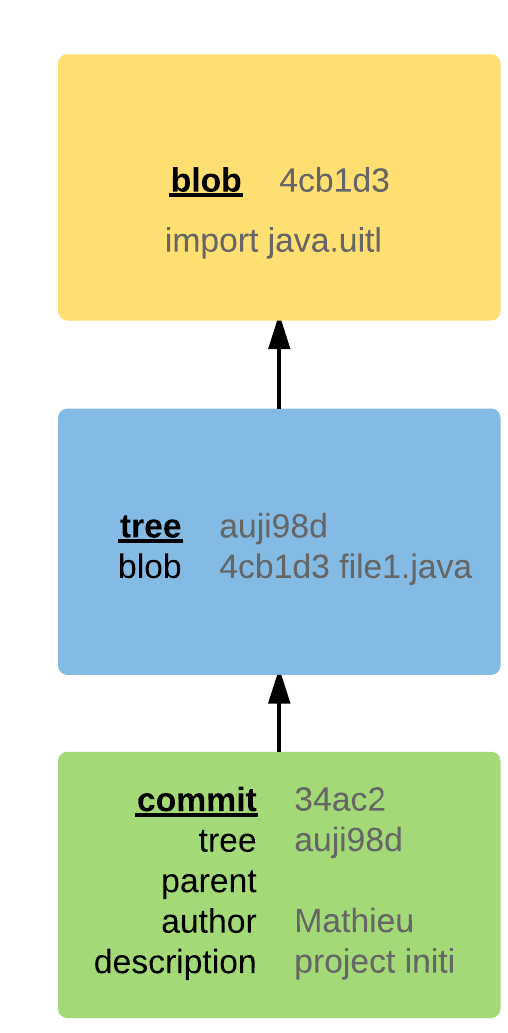
\includegraphics[scale=0.25]{media/commit-datastructure.png}
    \caption{Data structure of a commit.
    \label{fig:branching}}
\end{figure}

In this example, we can see that author ``Mathieu'' has created the file
\lstinline!file1.java! with the message ``project init''. Figure
\ref{fig:two-commits} represents an external modification. In this
second example, \lstinline!file1.java! is modified while
\lstinline!file2.java! is created. The second commit \lstinline!98ca9!
have \lstinline!34ac2! as a parent.

\begin{figure}[h!]
  \centering
    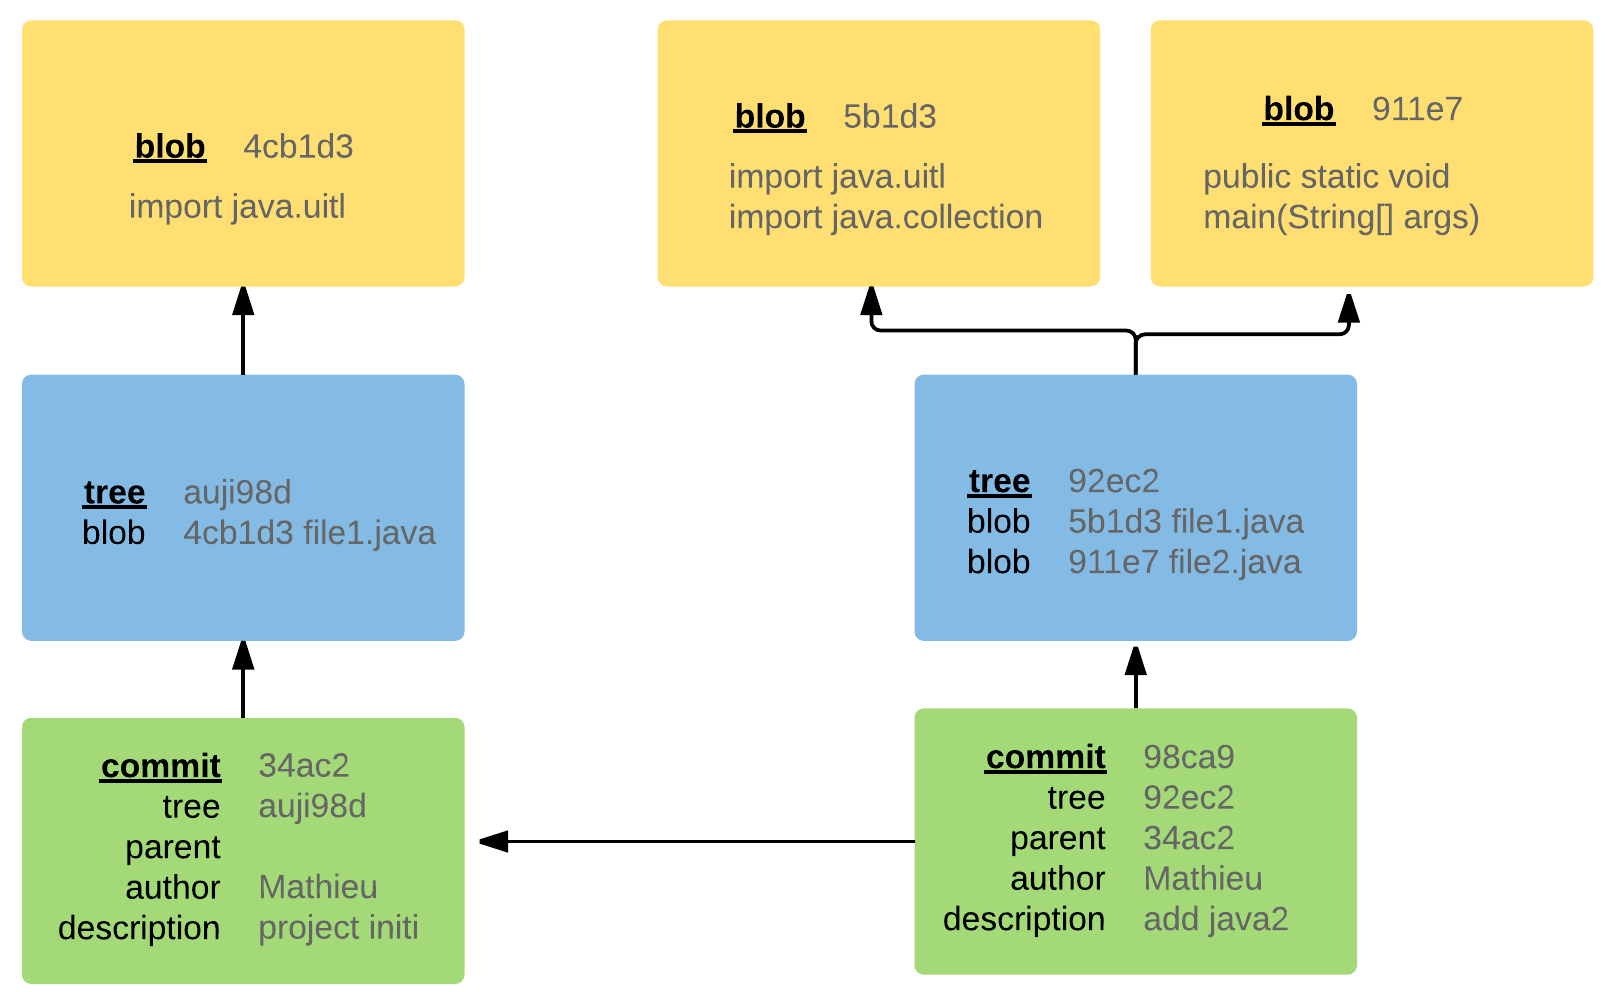
\includegraphics[scale=0.25]{media/branching.png}
    \caption{Data structure of two commits.
    \label{fig:two-commits}}
\end{figure}

Branches point to a commit. In a task-branching environment, a branch is
created via a checkout operation for each task. Tasks can be to fix the
root cause of a crash or bug report or features to implement. In figure
\ref{fig:two-branches}, the \lstinline!master! branch and the
\lstinline!1_fix_overflow! point on commit \lstinline!98ca9!.

\begin{figure}[h!]
  \centering
    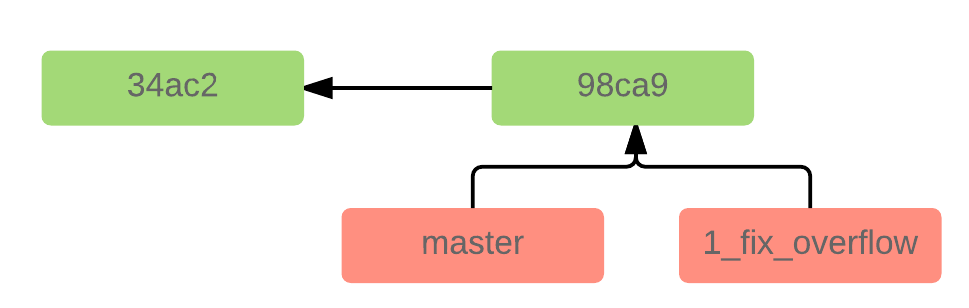
\includegraphics[scale=0.25]{media/2branches.png}
    \caption{Two branches pointing on one commit.
    \label{fig:two-branches}}
\end{figure}

Both branches can evolve separately and be merged when the task branch
is ready. In Figure \ref{fig:merge}, the \lstinline!master! branch
points on \lstinline!a13ab2! while the \lstinline!1_fix_overflow! points
on \lstinline!ahj23k!.

\begin{figure}[h!]
  \centering
    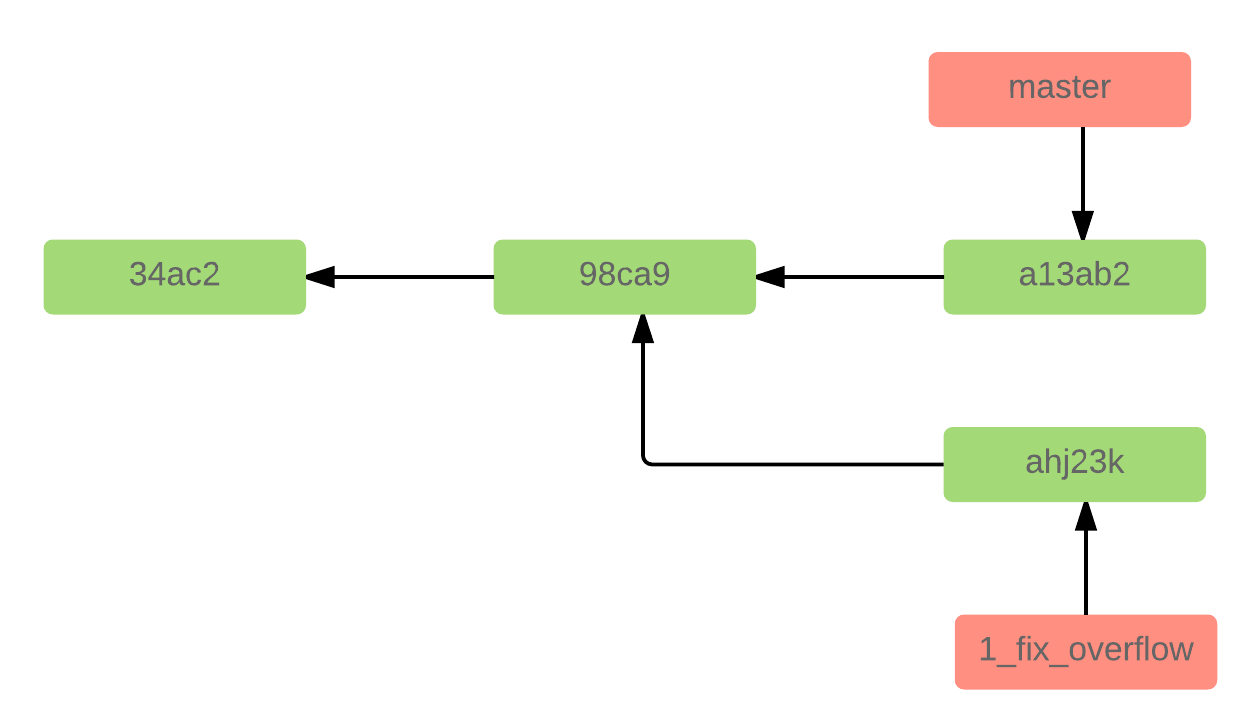
\includegraphics[scale=0.25]{media/merge.png}
    \caption{Two branches pointing on two commits.
    \label{fig:merge}}
\end{figure}

\section{\texorpdfstring{Providers\label{sec:revision-provider}}{Providers}}\label{providers}

In this proposal, we mainly refer to three version control systems:
\lstinline!Svn!, \lstinline!Git! and, to a lesser extent,
\lstinline!Mercurial!. \lstinline!SVN! is distributed by the Apache
Foundation and is a centralized concurrent version system that can
handle conflicts in the different versions of different developers. SVN
is widely used in industry. At the opposite, \lstinline!Git! is a
distributed revision control system --- originally developed by Linus
Torvald --- where revisions can be kept locally for a while and then
shared with the rest of the team. Finally, \lstinline!Mercurial! is also
a distributed revision system, but shares many concepts with
\lstinline!SVN!. It will be easier for people who are used to
\lstinline!SVN! to switch to a distributed revision system if they use
\lstinline!Mercurial!.

\subsection{Project Tracking Systems\label{sec:issue-tracking}}

Project tracking systems allow end users to create bug reports (BRs) to
report unexpected system behaviour, managers can create tasks to drive
the evolution forward and crash report (CRs) can be automatically
created. These systems are also used by development teams to keep track
of the modifications induced by bugs, crash reports, and keep track of
the fixes.

\begin{figure}[h!]
    \centering
    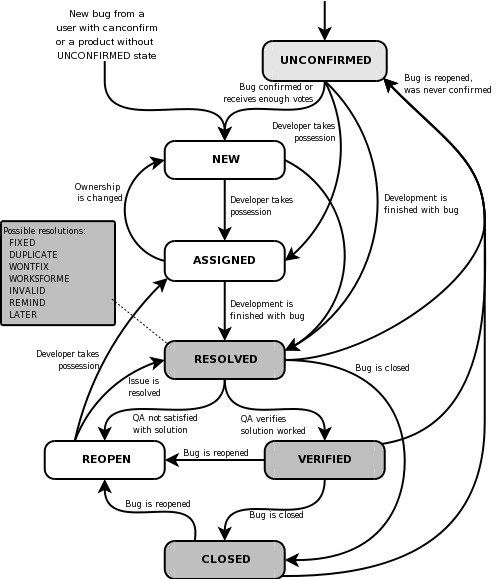
\includegraphics[scale=0.7]{media/bzLifecycle.png}
    \caption{Lifecyle of a report}
    \label{fig:bug-lifecyle}
\end{figure}

Figure \ref{fig:bug-lifecyle} presents the life cycle of a report
{[}28{]}. When an end-user submits a report, it is set to the
\lstinline!UNCONFIRMED! state until it receives enough votes or that a
user with the proper permissions modifies its status to \lstinline!NEW!.
The report is then assigned to a developer to be fixed. When the report
is in the \lstinline!ASSIGNED! state, the assigned developer(s) starts
working on the report. A fixed report moves to the \lstinline!RESOLVED!
state. Developers have five different possibilities to resolve a report:
\lstinline!FIXED!, \lstinline!DUPLICATE!, \lstinline!WONTFIX!,
\lstinline!WORKSFORME! and \lstinline!INVALID! {[}105{]}.

\begin{itemize}
\tightlist
\item
  RESOLVED/FIXED: A modification to the source code has been pushed,
  i.e., a changeset (also called a patch) has been committed to the
  source code management system and fixes the root problem described in
  the report.
\item
  RESOLVED/DUPLICATE: A previously submitted report is being processed.
  The report is marked as a duplicate of the original report.
\item
  RESOLVED/WONTFIX: This is applied in the case where developers decide
  that a given report will not be fixed.
\item
  RESOLVED/WORKSFORME: If the root problem described in the report
  cannot be reproduced on the reported OS/hardware.
\item
  RESOLVED/INVALID: If the report is not related to the software itself.
\end{itemize}

Finally, the report is \lstinline!CLOSED! after it is resolved. A report
can be reopened (sent to the \lstinline!REOPENED! state) and then
assigned again if the initial fix was not adequate (the fix did not
resolve the problem). The elapsed time between the report marked as the
new one and the resolved status is known as the \emph{fixing time},
usually in days. In case of task branching, the branch associated with
the report is marked as ready to be merged. Then, the person in charge
(quality assurance team, manager, ect\ldots{}) will be able to merge the
branch with the mainline. If the report is reopened: the days between
the time the report is reopened and the time it is marked again as
\lstinline!RESOLVED/FIXED! are cumulated. Reports can be reopened many
times.

Tasks follow a similar life cycle with the exception of the
\lstinline!UNCONFIRMED! and \lstinline!RESOLVED! states. Tasks are
created by management and do not need to be confirmed to be
\lstinline!OPEN! and \lstinline!ASSIGNED! to developers. When a task is
complete, it will not go to the \lstinline!RESOLVED! state, but to the
\lstinline!IMPLEMENTED! state. Bug and crash reports are considered as
problems to eradicate in the program. Tasks are considered as new
features or amelioration to include in the program.

Reports and tasks can have a severity associated with them {[}22{]}. The
severity indicates the degree of impact on the software system. The
possible severities are:

\begin{itemize}
\tightlist
\item
  blocker: blocks development and/or testing work.
\item
  critical: crashes, loss of data, severe memory leak.
\item
  major: major loss of function.
\item
  normal: regular report, some loss of functionality under specific
  circumstances.
\item
  minor: minor loss of function, or other problem where easy workaround
  is present.
\item
  trivial: cosmetic problems like misspelled words or misaligned text.
\end{itemize}

The relationship between a report or a task and the actual modification
can be hard to establish, and it has been a subject of various research
studies (e.g., {[}2, 12, 202{]}). The reason is that they are on two
different systems: the version control system and the project tracking
system. While it is considered a good practice to link each report with
the versioning system by indicating the report \lstinline!#id! on the
modification message, more than half of the reports are not linked to a
modification {[}202{]}.

\section{\texorpdfstring{Providers\label{sec:bug-provider}}{Providers}}\label{providers-1}

We have collected data from four different project tracking systems:
\lstinline!Bugzilla!, \lstinline!Jira!, \lstinline!Github! and
\lstinline!Sourceforge!. \lstinline!Bugzilla! belongs to the Mozilla
foundation and has first been released in 1998. \lstinline!Jira!,
provided by Altassian, has been released 14 years ago, in 2002.
\lstinline!Bugzilla! is 100\% open source and it is difficult to
estimate how many projects use it. However, we can envision that it owns
a great share of the market as major organizations such as Mozilla,
Eclipse and the Apache Software Foundation use it. \lstinline!Jira!, on
the other hand, is a commercial software tool --- with a freemium
business model --- and Altassian claims that they have 25,000 customers
over the world.

\lstinline!Github! and \lstinline!Sourceforge! are different from
\lstinline!Bugzilla! and \lstinline!Jira! in a sense that they were
created as source code revision systems and evolved, later on, to add
project tracking capabilities to their software tools. This common
particularity has the advantage to ease the link between bug reports and
the source code.

\chapter{Related work}\label{related-work}

\section{Clone Detection}\label{clone-detection}

Clone detection is an important and difficult task. Throughout the
years, researchers and practitioners have developed a considerable
number of methods and tools to efficiently detect source code clones. In
this section, we first describe the classical clone detection approaches
and then present works that focus on local and remote detection.

\subsection{Traditional Clone Detection
Techniques}\label{traditional-clone-detection-techniques}

Tree-matching and metric-based methods are two sub-categories of
syntactic analysis for clone detection. Syntactic analyses consist of
building abstract syntax trees (AST) and analyze them with a set of
dedicated metrics or searching for identical sub-trees. Many existing
AST-based approaches rely on sub-tree comparison to detect clone,
including the work of Baxter et al.{[}18{]}, Wahleret et al. {[}195{]},
and the work of Jian et al. with Deckard {[}82{]}. An AST-based approach
compares metrics computed on the AST, rather than the code itself, to
identify clones {[}15, 154{]}.

Text-based techniques use the code and compare sequences of code blocks
to each other to identify potential clones. Johnson was perhaps the
first one to use fingerprints to detect clones {[}86, 87{]}. Blocks of
code are hashed, producing fingerprints that can be compared. If two
blocks share the same fingerprint, they are considered as clones. Manber
et al. {[}121{]} and Ducasse et al. {[}48{]} refined the fingerprint
technique by using leading keywords and dot-plots.

Another approach for detecting clones is to use static analysis and to
leverage the semantics of a program to improve the detection. These
techniques rely on program dependency graphs, where nodes are statements
and edges are dependencies. Then, the problem of finding clones is
reduced to the problem of finding identical sub-groups in the program
dependency graph. Examples of existing techniques that fall into this
category are the ones presented by Krinke et al.{[}107{]} and Gabel et
al. {[}60{]}.

Many clone detection tools resort to lexical approaches for clone
detection. Here, the code is transformed into a series of tokens. If
sub-series repeat themselves, it means that a potential clone is in the
code. Some popular tools that use this technique include Dup {[}14{]},
CCFinder {[}92{]}, and CP-Miner {[}118{]}.

In 2010, Hummel et al. proposed an approach that is both incremental and
scalable using index-based clone detection {[}76{]}. Incremental clone
detection is a technique where only the changes from one version to
another are analysed. Thus, the required computational time is greatly
reduced. Using more than 100 machines in a cluster, they managed to drop
the computation time of Type 1 and 2 to less than a second while
comparing a new version. The time required to find all the clones on a
73 MLOC system was 36 minute. We reach similar performances, for one
revision, using a single machine. While being extremely fast and
reliable, Hummel et al.`s approach required an industrial cluster to
achieve such performance. In our opinion, it is unlikely that standard
practitioners have access to such computational power. Moreover, the
authors' approach only targets Type 1 and 2 clones. Higo et al. proposed
an incremental clone detection approach based on program dependency
graphs (PDG) {[}72{]}. Using PDG is arguably more complex than text
comparison and allows the detection of clone structures that are
scattered in the program. They were able to analyze 5,903 revisions in
15 hours in Apache Ant.

\subsection{Remote Detection of
Clones}\label{remote-detection-of-clones}

Yuki et al. conducted one of the few studies on the application of clone
management to industrial systems {[}204{]}. They implemented a tool
named Clone Notifier at NEC with the help of experienced practitioners.
They specifically focus on clone insertion notification, very much like
PRECINCT. Unlike PRECINCT, their approach uses a remote approach in
which the changes are committed (i.e., they reach the central
repository, and anyone can pull them into his or her machines) and a
central server analyses the changes. If the committed changes contain
newly inserted clones, then an email notification is sent.

Zhang et al. proposed CCEvents (Code Cloning Events) {[}211{]}. Their
approach monitors code repository continuously and allows stakeholders
to use a domain specific language called CCEML to specify which email
notifications they wish to receive.

In addition, many commercial tools now include clone detection as part
of continuous integration. Codeclimate \^{}codeclimate, Codacy
\^{}codacy, Scrutinizer \^{}scrutinizer and Coveralls\^{}coveralls are
some examples. These tools will perform various tasks such as executing
unit test suites, computing quality metricsm performing clone detection
and, provide a report by email.

We argue that remotely detecting clones is not practical because clones
can be synchronized by other team members, which may lead to challenging
merges when the clones are removed. In addition, the authors did not
report performance measurements and the longer it takes for the
notification to be sent to the developer, the harder it can be to
reconstruct the mind-map required for clone removal.

\subsection{Local Detection of Clones}\label{local-detection-of-clones}

Gode and Koschke {[}62{]} proposed an incremental clone detector that
relies on the results of analysis from past versions of a system to only
analyze the new changes. Their clone detector takes the form of an IDE
plugin that alerts developers as soon as a clone is inserted into the
program.

Zibran and Roy {[}214, 215{]} proposed another IDE-based clone
management system to detect and refactor near-miss clones for Eclipse.
Their approach uses a k-difference hybrid suffix tree algorithm. It can
detect clones in real-time and propose a semi-automated refactoring
process.

Robert el al. {[}180{]} proposed another IDE plugin for Eclipse called
CloneDR based on ASTs that introduced novel visualization for clone
detection such as scatter-plots.

IDE-based methods tend to issue many warnings to developers that may
interrupt their work, hence hindering their productivity {[}103{]}. In
addition, Latoza et al. {[}112{]} found that there exist six different
reasons that trigger the use of clones (e.g., copy and paste of code
examples, reimplementations of the same functionality in different
languages, etc. ). Developers are aware that they are creating clones in
five out of six situations. In such cases, warnings provided by
IDE-based local detection techniques can be quite disturbing.

Nguyen et al. {[}146{]} proposed an advanced clone-aware source code
management system called Clever. Their approach uses abstract syntax
trees to detect, update, and manage clones. While efficient, their
approach does not prevent the introduction of clones, and it is not
incremental. Developers have to run a project-wide detection for each
version of the program. The same teams {[}145{]} conducted follow-up
study by making Clever incremental. Their new tool, JSync, is an
incremental clone detector that will only perform the detection of
clones on the new changes.

Niko el al. {[}147{]} proposed techniques revolving around hashing to
obtain a quick answer while detecting Type 1, Type 2, and Type 3 clones
in Squeaksource. While their approach works on a single system (i.e.,
detecting clones on one version of one system), they found that more
than 14\% of all clones are copied from project to project, stressing
the need for fast and scalable approaches for clone detection to detect
clone across a large number of projects. On the performance side, Niko
el al. were able to perform clone detection on 74,026 classes in 14:45
hours (4,747 class per hour) with an eight core Xeon at 2.3 GHz with 16
GB of RAM. While these results are promising, especially because the
approach detects clones across projects and versions, the computing
power required is still considerable.

Similarly, Saini et al. {[}169{]} and Sajnani et al. {[}170{]} proposed
an approach, called SourcererCC. SourcererCC targets fast clone
detection on developers' workstation (12 GB RAM). SourcererCC is a
token-based clone detector that uses an optimized inverted-index. It was
tested on 25K projects cumulating 250 MLOC. The technique achieves a
precision of 86\% and a recall of 86\%-100\% for clones of Type 1, 2 and
3.

Toomey el al. {[}189{]} also proposed an efficient token based approach
for detecting clones called ctcompare. Their tokenization is, however,
different than most approaches as they used lexical analysis to produce
sequences of tokens that can be transformed into token tuples. ctcompare
is accurate, scalable and fast but does not detect Type 3 clones.

\section{Reports and source code
relationships}\label{reports-and-source-code-relationships}

Mining bug repositories is perhaps one of the most active research
fields today. The reason is that the analysis of bug reports (BRs)
provides useful insight that can help with many maintenance activities
such as bug fixing {[}168, 198{]} bug reproduction {[}9, 32, 83{]},
fault analysis {[}142{]}, etc. This increase of attention can be further
justified by the emergence of many open source bug tracking systems,
allowing software teams to make their bug reports available online to
researchers.

These studies, however, treat all bugs as the same. For example, a bug
that requires only one fix is analyzed the same way as a bug that
necessitates multiple fixes. Similarly, if multiple bugs are fixed by
modifying the exact same locations in the code, then we should
investigate how these bugs are related in order to predict them in the
future.

Researchers have been studying the relationships between the bug and
source code repositories since more than two decades. To the best of our
knowledge, the first ones who conducted this type of study on a
significant scale were Perry and Stieg {[}155{]}. In these two decades,
many aspects of these relationships have been studied in length. For
example, researchers were interested in improving the bug reports
themselves by proposing guidelines {[}22{]}, and by further simplifying
existing bug reporting models {[}71{]}.

Another field of study consists of assigning these bug reports,
automatically if possible, to the right developers during triaging {[}3,
25, 81, 181{]}. Another set of approaches focus on how long it takes to
fix a bug {[}24, 168, 212{]} and where it should be fixed {[}208,
213{]}. With the rapidly increasing number of bugs, the community was
also interested in prioritizing bug reports {[}97{]}, and in predicting
the severity of a bug {[}110{]}. Finally, researchers proposed
approaches to predict which bug will get reopened {[}119, 217{]}, which
bug report is a duplicate of another one {[}23, 79, 186{]} and which
locations are likely to yield new bugs {[}99, 101{]}.

\section{Fault Prediction}\label{fault-prediction}

The majority of previous file/module-level prediction work used code or
process metrics. Approaches using code metrics only use information from
the code itself and do not use any historical data. Chidamber and
Kemerer published the well-known CK metrics suite {[}34{]} for object
oriented designs and inspired Moha et al. to publish similar metrics for
service-oriented programs {[}128{]}. Another famous metric suite for
assessing the quality of a given software design is Briand's coupling
metrics {[}26{]}.

The CK and Briand's metrics suites have been used, for example, by
Basili et al. {[}16{]}, El Emam et al. {[}53{]}, Subramanyam et al.
{[}176{]} and Gyimothy et al. {[}64{]} for object-oriented designs.
Service oriented designs have been far less studied than object oriented
design as they are relatively new, but, Nayrolles et al. {[}140, 141{]},
Demange et al. {[}47{]} and Palma et al. {[}152{]} used Moha et al.
metric suites to detect software defects. All these approaches, proved
software metrics to be useful at detecting software fault for object
oriented and service oriented designs, respectively. More recently,
Nagappan et al. {[}129, 131{]} and Zimmerman et al. {[}216, 218{]}
further refined metrics-based detection by using statical analysis and
call-graph analysis.

Other approaches use historical development data, often referred to as
process metrics. Naggapan and Ball {[}130{]} studied the feasibility of
using relative churn metrics to prediction buggy modules in the Windows
Server 2003. Other work by Hassan et al. and Ostrand et al. used past
changes and defects to predict buggy locations (e.g., {[}66{]},
{[}151{]}). Hassan and Holt proposed an approach that highlights the top
ten most susceptible locations to have a bug using heuristics based on
file-level metrics {[}66{]}. They find that locations that have been
recently modified and fixed locations are the most defect-prone.
Similarly, Ostrand et al. {[}151{]} predict future crash location by
combining the data from changed and past defect locations. They validate
their approach on industrial systems at AT\&T. They showed that data
from prior changes and defects can effectively predict defect-prone
locations for open-source and industrial systems. Kim et al. {[}101{]}
proposed the bug cache approach, which is an improved technique over
Hassan and Holt's approach {[}66{]}. Rahman and Devanbu found that, in
general, process-based metrics perform as good as or better than
code-based metrics {[}159{]}.

Other work focused on the prediction of risky changes. Kim et al.
proposed the change classification problem, which predicts whether a
change is buggy or clean {[}178{]}. Hassan {[}67{]} used the entropy of
changes to predict risky changes. They find that the more complex a
change is, the more likely it is to introduce a defect. Kamei et al.
performed a large-scale empirical study on change classification
{[}91{]}. The studies above find that size of a change and the history
of the files being changed (i.e., how buggy they were in the past) are
the best indicators of risky changes.

\section{Automatic Patch Generation}\label{automatic-patch-generation}

Pan et al. {[}153{]} identified 27 bug fixing patterns that can be
applied to fix software bugs in Java programs. They showed that between
45.7 - 63.6\% of the bugs could be fixed with their patterns. Later, Kim
et al. {[}96{]} generated patches from human-written patches and showed
that their tool, PAR, successfully generated patches for 27 of 119 bugs.
Tao et al. {[}182{]} also showed that automatically generated patches
can assist developers in debugging tasks. Other work also focused on
determining how to best generate acceptable and high quality patches,
e.g. {[}42, 114{]}, and determine what bugs are best fit for automatic
patch generation {[}115{]}.

Our work differs from the work on automated patch generation in that we
do not generate patches; rather we use clone detection to determine the
similarity of a change to a previous risky change and suggest to the
developer the fixes of the prior risky changes.

\section{Crash Reproduction}\label{crash-reproduction}

In this section, we put the emphasis on how crash traces are used in
crash reproduction tasks. Existing studies can be divided into two
distinct categories: (A) on-field record and in-house replay techniques
{[}9, 133, 162, 175{]}, and (B) on-house crash understanding {[}31, 83,
84, 137, 219{]}.

These two categories yield varying results depending on the selected
approach and are mainly differentiated by the need for instrumentation.
The first category of techniques oversees -- by means of instrumentation
-- the execution of the target system on the field in order to reproduce
the crashes in-house, whereas tools and approaches belonging to the
second category only use data produced by the crash such as the crash
stack or the core dump at crash time. In the first category, tools
record different types of data such as the invoked methods {[}133{]},
try-catch exceptions {[}164{]}, or objects {[}80{]}. In the second
category, existing tools and approaches are aimed towards understanding
the causes of a crash, using data produced by the crash itself, such as
a crash stack {[}31{]}, previous -- and controlled -- execution
{[}219{]}, etc.

Tools and approaches that rely on instrumentation face common
limitations such as the need to instrument the source code in order to
introduce logging mechanisms{[}9, 80, 133{]}, which is known to slow
down the subject system. In addition, recording system behavior by means
of instrumentation may yield privacy concerns. Tools and approaches that
only use data about a crash -- such as core dump or exception stack
crashes -- face a different set of limitations. They have to reconstruct
the timeline of events that have led to the crash {[}31, 137{]}.
Computing all the paths from the initial state of the software to the
crash point is an NP-complete problem, and may cause state space
explosion {[}31, 36{]}.

In order to overcome these limitations, some researchers have proposed
to use various SMT (satisfiability modulo theories) solvers {[}49{]} and
model checking techniques {[}193{]}. However, these techniques require
knowledge that goes beyond traditional software engineering, which
hinders their adoption {[}194{]}.

It is worth mentioning that both categories share a common limitation.
It is possible for the required condition to reproduce a crash to be
purely external such as the reading of a file that is only present on
the hard drive of the customer or the reception of a faulty network
packet {[}31, 137{]}. It is almost impossible to reproduce the bug
without this input.

\subsection{On-field Record and In-house
Replay}\label{on-field-record-and-in-house-replay}

Jaygarl et al. created OCAT (Object Capture based Automated Testing)
{[}80{]}. The authors' approach starts by capturing objects created by
the program when it runs on-field in order to provide them with an
automated test process. The coverage of automated tests is often low due
to lack of correctly constructed objects. Also, the objects can be
mutated by means of evolutionary algorithms. These mutations target
primitive fields in order to create even more objects and, therefore,
improve the code coverage. While not directly targeting the reproduction
of a bug, OCAT is an approach that was used as the main mechanism for
bug reproduction systems.

Narayanasamy et al. {[}133{]} proposed BugNet, a tool that continuously
records program execution for deterministic replay debugging. According
to the authors, the size of the recorded data needed to reproduce a bug
with high accuracy is around 10MB. This recording is then sent to the
developers and allows the deterministic replay of a bug. The authors
argued that with nowadays Internet bandwidth the size of the recording
is not an issue during the transmission of the recorded data.

Another approach in this category was proposed by Clause et al.
{[}36{]}. The approach records the execution of the program on the
client side and compresses the generated data. Moreover, the approach
keeps compressed traces of all accessed documents in the operating
system. This data is sent to the developers to replay the execution of
the program in a sandbox, simulating the client's environment. This
special feature of the approach proposed by Clause et al. addresses the
limitation where crashes are caused by external causes. While the
authors broaden the scope of reproducible bugs, their approach records a
lot of data that may be deemed private such as files used for the proper
operation of the operating system.

Timelapse {[}29{]} also addresses the problem of reproducing bugs using
external data. The tool focuses on web applications and allows
developers to browse and visualize the execution traces recorded by
Dolos. Dolos captures and reuses user inputs and network responses to
deterministically replay a field crash. Also, both Timelapse and Dolos
allow developers to use conventional tools such as breakpoints and
classical debuggers. Similar to the approach proposed by Clause et al.
{[}36{]}, private data are recorded without obfuscation of any sort.

Another approach was proposed by Artzi et al. and named ReCrash. ReCrash
records the object states of the targeted programs {[}9{]}. The authors
use an in-memory stack, which contains every argument and object clone
of the real execution in order to reproduce a crash via the automatic
generation of unit test cases. Unit test cases are used to provide hints
to the developers about the buggy code. This approach particularly
suffers from the limitation related to slowing down the execution. The
overhead for full monitoring is considerably high (between 13\% and 64\%
in some cases). The authors propose an alternative solution in which
they record only the methods surrounding the crash. For this to work,
the crash has to occur at least once so they could use the information
causing the crash to identify the methods surrounding it.ReCrash was
able to reproduce 100\% (11/11) of the submitted bugs.

Similar to ReCrash, JRapture {[}175{]} is a capture/replay tool for
observation-based testing. The tool captures the execution of Java
programs to replay it in-house. To capture the execution of a Java
program, the creators of JRapture used their own version of the Java
Virtual Machine (JVM) and a lightweight, transparent capture process.
Using a customized JVM allows capturing any interactions between a Java
program and the system including GUI, files, and console inputs. These
interactions can be replayed later with exactly the same input sequence
as seen during the capture phase. However, using a custom JVM is not a
practical solution. This is because the authors' approach requires users
to install a JVM that might have some discrepancies with the original
one and yield bugs if used with other software applications. In our
view, JRapture fails to address the limitations caused by
instrumentation because it imposes the installation of another JVM that
can also monitor other software systems than the intended ones. RECORE
(REconstructing CORE dumps) is a tool proposed by Robler et al. The tool
instruments Java byte code to wrap every method in a try-catch block
while keeping a quasi-null overhead {[}164{]}. RECORE starts from the
core dump and tries (with evolutionary algorithms) to reproduce the same
dump by executing the subject program many times. When the generated
dump matches the collected one, the approach has found the set of inputs
responsible for the failure and was able to reproduce 85\% (6/7) of the
submitted bugs.

The approaches presented at this point operate at the code level. There
exist also techniques that focus on recording user-GUI interactions
{[}70, 162{]}. Roehm et al. extract the recorded data using delta
debugging {[}209{]}, sequential pattern mining, and their combination to
reproduce between 75\% and 90\% of the submitted bugs while pruning 93\%
of the actions.

Among the approaches presented here, only the ones proposed by Clause et
al. and Burg et al. address the limitations incurred due to the need for
external data at the cost, however, of privacy. To address the
limitations caused by instrumentation, the RECORE approach proposes to
let users choose where to put the bar between the speed of the subject
program, privacy, and bug reproduction efficiency. As an example, users
can choose to contribute or not to improving the software -- policy
employed by many major players such as Microsoft in Visual Studio or
Mozilla in Firefox -- and propose different types of monitoring where
the cost in terms of speed, privacy leaks, and efficiency for
reproducing the bug is clearly explained.

\subsection{On-house Crash
Explanation}\label{on-house-crash-explanation}

On the other side of the picture, we have tools and approaches belonging
to the on-house crash explanation (or understanding), which are fewer
but newer than on-field record and replaying tools.

Jin et al. proposed BugRedux for reproducing field failures for in-house
debugging {[}83{]}. The tool aims to synthesize in-house executions that
mimic field failures. To do so, the authors use several types of data
collected in the field such as stack traces, crash stack at points of
failure, and call sequences. The data that successfully reproduced the
field crash is sent to software developers to fix the bug. BugRedux
relies on several in-house executions that are synthesized so as to
narrow down the search scope, find the crash location, and finally
reproduce the bug. However, these in-house executions have to be
conducted before the work on the bug really begins. Also, the in-house
executions suffer from the same limitation as unit testing, i.e., the
executions are based on the developer's knowledge and ability to develop
exceptional scenarios in addition to the normal ones. Based on the
success of BugRedux, the authors built F3 (Fault localization for Field
Failures) {[}84{]} and MIMIC {[}219{]}. F3 performs many executions of a
program on top of BugRedux in order to cover different paths that are
leading to the fault. It then generates many \emph{pass} and \emph{fail}
paths, which can lead to a better understanding of the bug. They also
use grouping, profiling and filtering, to improve the fault localization
process. MIMIC further extends F3 by comparing a model of correct
behavior to failing executions and identifying violations of the model
as potential explanations for failures.

While being close to our approach, BugRedux and F3 may require the call
sequence and/or the complete execution trace in order to achieve bug
reproduction. When using only the crash traces (referred to as call
stack at crash time in their paper), the success rate of BugRedux
significantly drops to 37.5\% (6/16). The call sequence and the complete
execution trace required to reach 100\% accuracy can only be obtained
through instrumentation and with an overhead ranging from 10\% to
1066\%. Chronicle {[}20{]} is an approach that supports remote debugging
by capturing inputs in the application through code instrumentation. The
approach seems to have a low overhead on the instrumented application,
around 10\%.

Likewise, Zamfir et al. proposed ESD {[}206{]}, an execution synthesis
approach that automatically synthesizes failure execution using only the
stack trace information. However, this stack trace is extracted from the
core dump and may not always contain the components that caused the
crash.

To the best of our knowledge, the most complete work in this category is
the one of Chen in his PhD thesis {[}31{]}. Chen proposed an approach
named STAR (Stack Trace based Automatic crash Reproduction). Using only
the crash stack, STAR starts from the crash line and goes backward
towards the entry point of the program. During the backward process,
STAR computes the required condition using an SMT solver named Yices
{[}49{]}. The objects that satisfy the required conditions are generated
and orchestrated inside a JUnit test case. The test is run, and the
resulting crash stack is compared to the original one. If both match,
the bug is said to be reproduced. STAR aims to tackle the state
explosion problem of reproducing a bug by reconstructing the events in a
backward fashion and therefore saving numerous states to explore. STAR
was able to reproduce 38 bugs out of 64 (54.6\%). Also, STAR is
relatively easy to implement as it uses Yices {[}49{]} and potentially
Z3 {[}45{]} (stated in their future work) that are well-supported SMT
solvers.

Except for STAR, existing approaches that target the reproduction of
field crashes require the instrumentation of the code or the running
platform in order to save the stack call or the objects to successfully
reproduce bugs. As we discussed earlier, such approaches yield good
results 37.5\% to 100\%, but the instrumentation can cause a massive
overhead (1\% to 1066\%) while running the system. In addition, the data
generated at run-time using instrumentation may contain sensitive
information.

\section{Bugs Classification}\label{bugs-classification}

Researchers have been studying the relationships between the bug and
source code repositories for more than two decades. To the best of our
knowledge, the first ones who conducted this type of study on a
significant scale were Perry and Stieg {[}155{]}. In these two decades,
many aspects of these relationships have been studied in length. For
example, researchers were interested in improving the bug reports
themselves by proposing guidelines {[}22{]}, and by further simplifying
existing bug reporting models {[}71{]}.

Another field of study consists of assigning these bug reports,
automatically if possible, to the right developers during triaging {[}3,
25, 81, 181{]}. Another set of approaches focus on how long it takes to
fix a bug {[}24, 168, 212{]} and where it should be fixed {[}208,
213{]}. With the rapidly increasing number of bugs, the community was
also interested in prioritizing bug reports {[}97{]}, and in predicting
the severity of a bug {[}110{]}. Finally, researchers proposed
approaches to predict which bug will get reopened {[}119, 217{]}, which
bug report is a duplicate of another one {[}23, 79, 186{]} and which
locations are likely to yield new bugs {[}99, 102, 191{]}. However, to
the best of our knowledge, there are not many attempts to classify bugs
the way we present in this paper. In her PhD thesis {[}54{]}, Sigrid
Eldh discussed the classification of trouble reports concerning a set of
fault classes that she identified. Fault classes include computational
logical faults, ressource faults, function faults, etc. She conducted
studies on Ericsson systems and showed the distributions of trouble
reports with respect to these fault classes. A research paper was
published on the topic in {[}54{]}. or safety critical{[}65{]}. Hamill
et al.{[}65{]} proposed a classification of faults and failures in
critical safety systems. They proposed several types of faults and
showed how failures in critical safety systems relate to these classes.
They found that only a few fault types were responsible for the majority
of failures. They also compare on pre-release and post-release faults
and showed that the distributions of fault types differed for
pre-release and post-release failures. Another finding is that coding
faults are the most predominant ones.

Our study differs from theses studies in the way that we focus on the
bugs and their fixes across a wide range of systems, programming
languages, and purposes. This is done independently from a specific
class of faults (such as coding faults, resource faults, etc.). This is
because our aim is not to improve testing as it is the case in the work
of Eldh {[}54{]} and Hamill et al. {[}65{]}. Our objective is to propose
a classification that can allow researchers in the filed of mining bug
repositories to use the taxonomy as a new criterion in triaging,
prediction, and reproduction of bugs. By analogy, we can look at the
proposed bug taxonomy similarly to the clone taxonomy presented by
Kapser and Godfrey {[}95{]}. The authors proposed seven types of source
code clones and then conducted a case study, using their classification,
on the file system module of the Linux operating system. This clone
taxonomy continues to be used by researchers to build better approaches
for detecting a given clone type and being able to compare approaches
with each other effectively.

\chapter{An Aggregated Bug Repository for Developers and
Researchers}\label{an-aggregated-bug-repository-for-developers-and-researchers}

\section{Introduction}\label{introduction-1}

Program debugging, an important software maintenance activity, is known
to be challenging and labor-intensive. Studies have shown that the cost
of software maintenance can reach up to 70\% of the overall cost of the
software development process {[}157{]}.

When facing a new bug, one might want to leverage decades of open source
software history to find a suitable solution. The chances are that a
similar bug or crash has already been fixed somewhere in another open
source project. The problem is that each open source project hosts its
data in a different data repository, using different bug tracking and
version control systems. Moreover, these systems have different
interfaces to access data.

The data is not represented in a uniform way either. This is further
complicated by the fact that bug tracking tools and version control
systems are not necessarily connected. The former follows the life of
the bug, while the latter manages the fixes. As a general practice,
developers create a link between the bug report system and the version
control tool by either writing the bug \#ID in their commits message or
add a link towards the changeset as a comment in the bug report system.
As a result, one would have to search the version control system
repository to find candidate solutions.

Moreover, developers mainly use classical search engines that index
specialized sites such as
StackOverflow\footnote{http://stackoverflow.com/}. These sites are
organized in the form of question-response where a developer submits a
problem and receives answers from the community. While the answers are
often accurate and precise, they do not leverage the history of open
source software that has been shown to provide useful insights to help
with many maintenance activities such as bug fixing {[}168{]}, bug
reproduction {[}137{]}, fault analysis {[}142{]}, etc.

In this paper, we introduce BUMPER (BUg Metarepository for dEvelopers
and Researchers), a web-based infrastructure that can be used by
software developers and researchers to access data from diverse
repositories using natural language queries transparently, regardless of
where the data was originally created and hosted.

The idea behind BUMPER is that it can connect to any bug tracking and
version control systems and download the data into a single database. We
created a common schema that represents data, stored in various bug
tracking and version control systems. BUMPER uses a web-based interface
to allow users to search the aggregated database by expressing queries
through a single point of access. This way, users can focus on the
analysis itself and not on the way the data is represented or located.
BUMPER supports many features including: (1) the ability to use multiple
bug tracking and control version systems, (2) the ability to search very
efficiently large data repositories using both natural language and a
specialized query language, (3) the mapping between the bug reports and
the fixes, and (4) the ability to export the search results in Json, CSV
and XML formats.

\section{Approach}\label{approach}

\subsection{Architecture}\label{architecture}

Figure \ref{fig:bumper-architecture} shows the overall architecture of
BUMPER. BUMPER relies on a highly scalable architecture composed of two
Virtual Private Servers (VPS), hosted on a physical server.

\begin{figure}
  \centering
  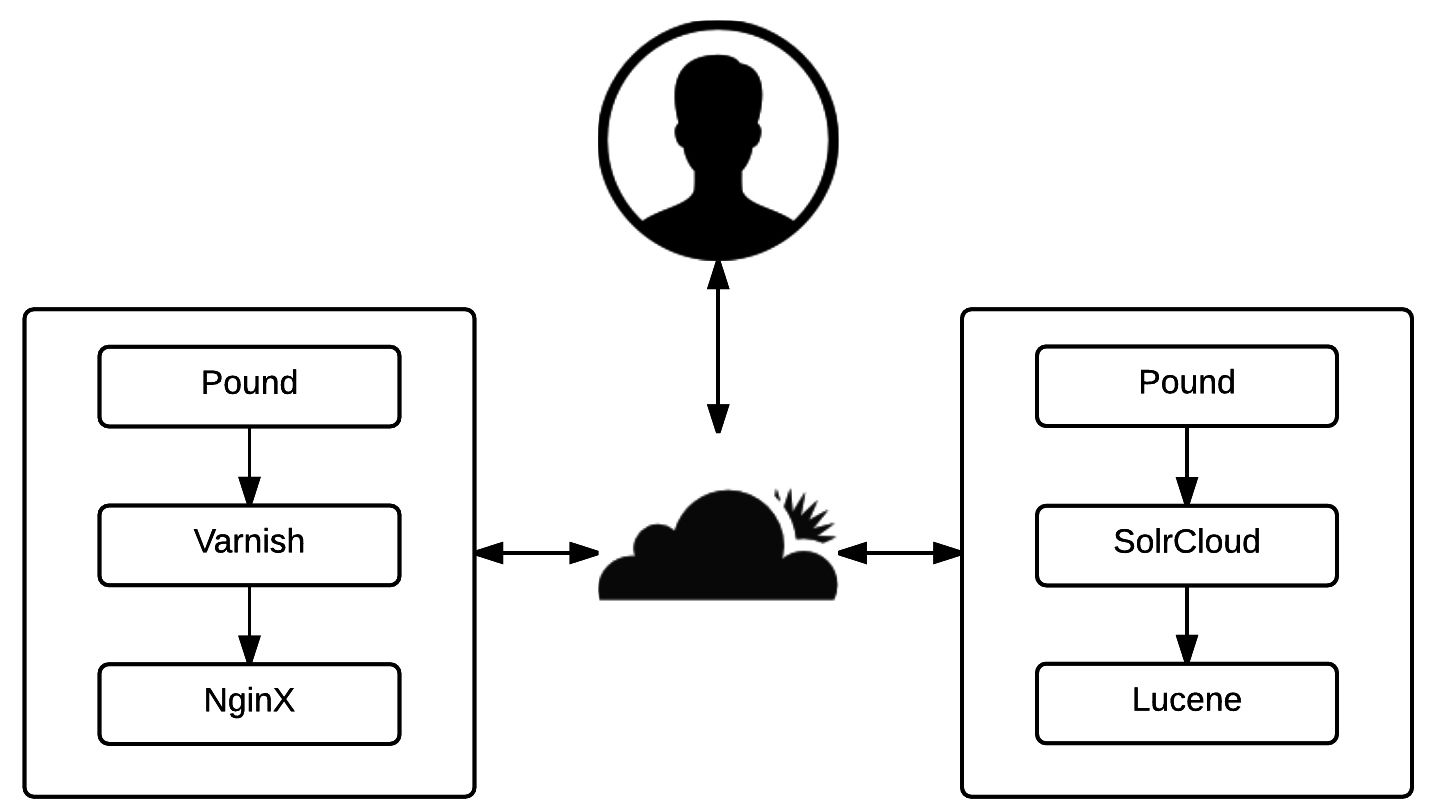
\includegraphics[width=0.7\textwidth]{media/archi.png}
  \caption{Bumper Architecture\label{fig:bumper-architecture}}
\end{figure}

The first server handles the web requests and runs three distinct
components: Pound, Varnish, and NginX. Pound is a lightweight open
source reverse proxy program and application firewall. It also serves to
decode https request to http. Translating an https request to http
allows us to save the https decryption time required on each step. Pound
also acts as a load-balancing service for the lower levels. Varnish then
handles the translated requests. Varnish is an http accelerator designed
for content-heavy and dynamic websites. It caches requests that come in
and serves the Web requests from the cache if the cache is still valid.
NginX (pronounced engine-x) is a web-server that was developed with a
particular focus on high concurrency, high performances, and low memory
usage. The second VPS also uses Pound for the same reasons and
SolrCloud. SolrCloud is the scalable version of Apache Solr where the
data can be separated into shards (e.g., chunks of manageable size).
Each shard can be hosted on a different server, but still indexed in a
central repository. Hence, we can guarantee a low query time despite the
large size of the data. Finally, Lucene is the full text search engine
powering Solr. This highly scalable architecture allows BUMPER to serve
requests in less than a second in average.

\subsection{\texorpdfstring{BUMPER
Metadata\label{sub:BUMPER Metadata}}{BUMPER Metadata}}\label{bumper-metadata}

Figure \ref{fig:bumper-metamodel} shows the core BUMPER metamodel, which
captures the common data elements used by most existing bug tracking and
control version systems. An issue (task) is characterized by a date, a
title, a description, and a fixing time.

\begin{figure*}
  \centering
  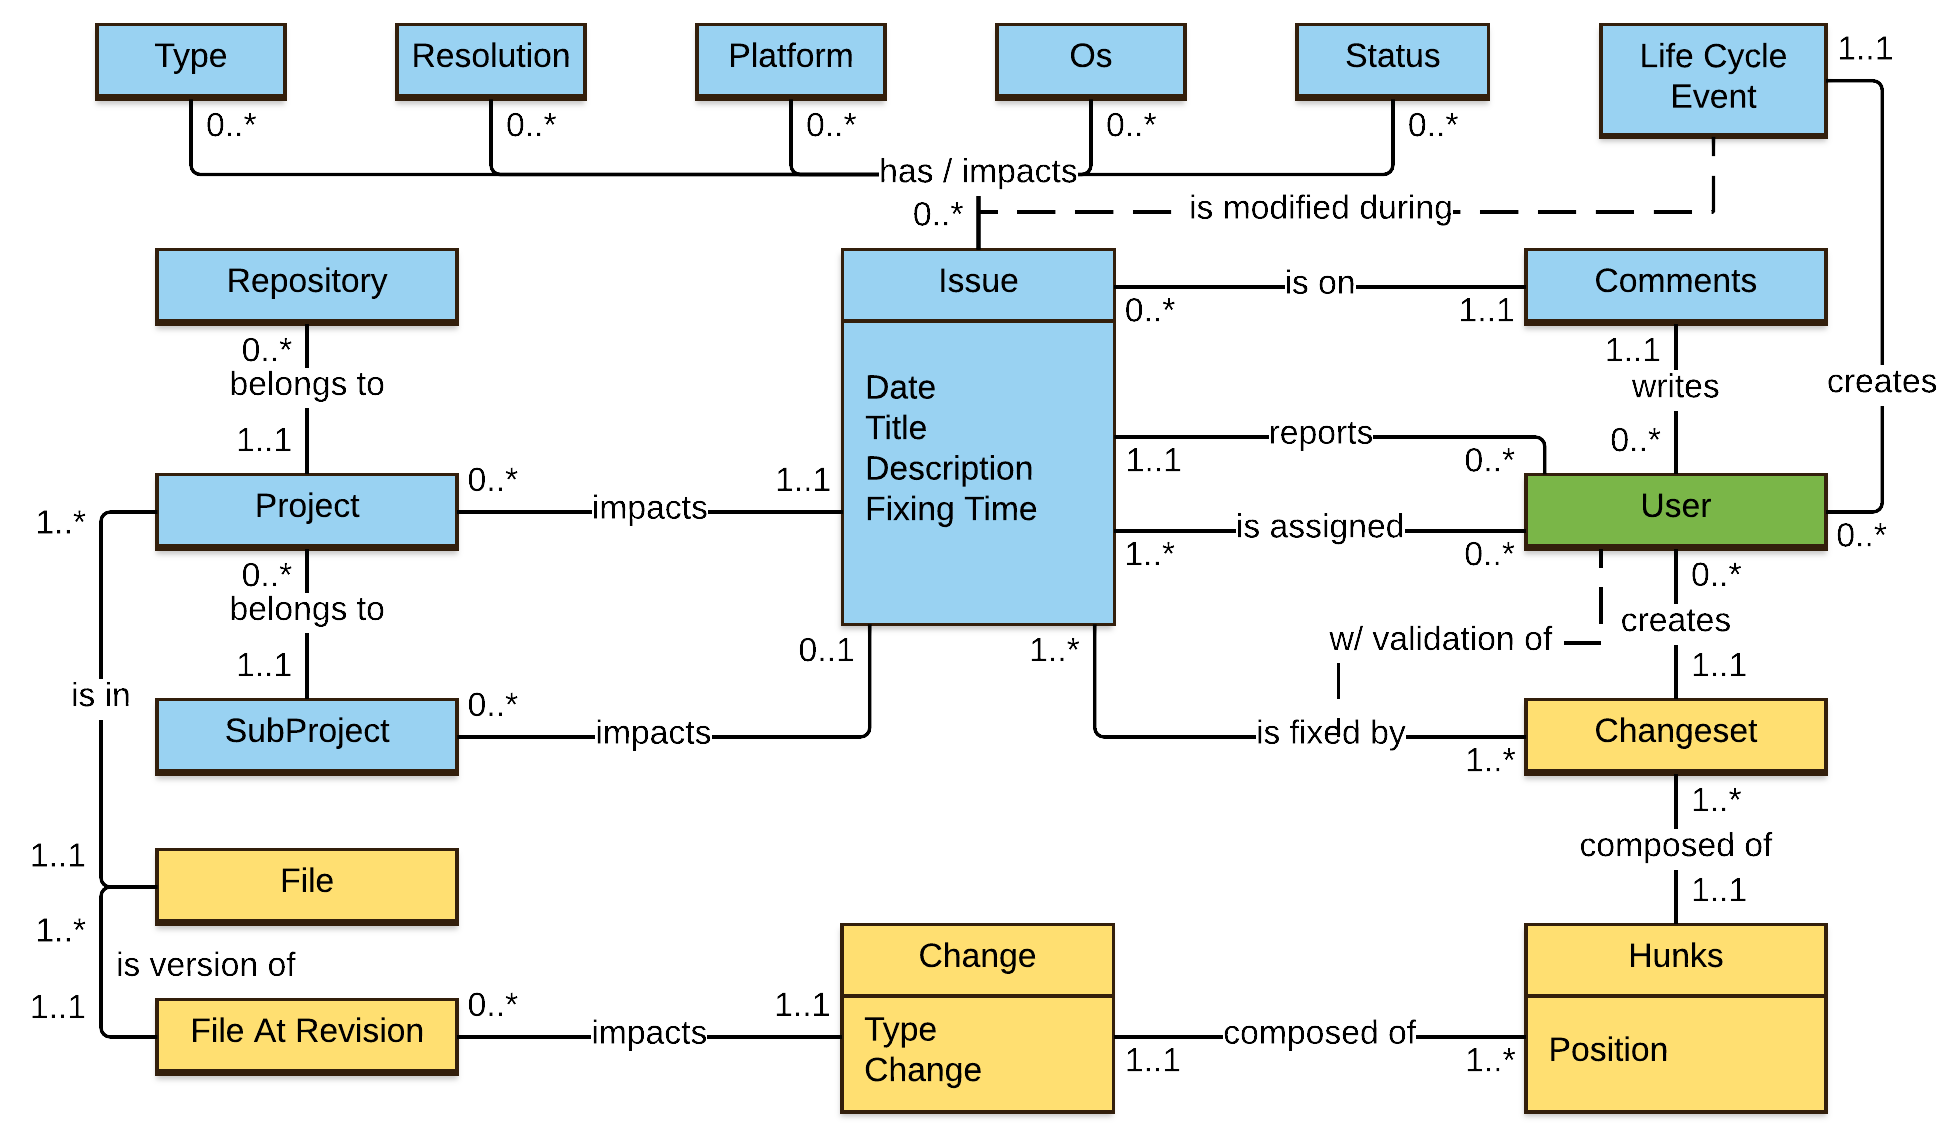
\includegraphics[width=0.95\textwidth]{media/bumper-model.png}
  \caption{BUMPER Metamodel\label{fig:bumper-metamodel}}
\end{figure*}

Issues are reported (created) by and assigned to users. Also, issues
belong to a project that is in a repository and might be composed of
subprojects. Users can modify an issue during life cycle events which
impact the type, the resolution, the platform, the OS and the status.
Issues are resolved (implemented) by changesets that are composed of
hunks. Hunks contain the actual changes to a file at a given revision,
which are versions of the file entity that belongs to a project.

In addition, BUMPER has different indexes over the data in order to
provide results efficiently. First of all, each feature of bug reports
and bug fixes (number of files, number of hunks, etc.) have their own
index. Furthermore, BUMPER has data indexes over the project name, the
sub-project name, the programming language, etc. Finally, two major
indexes are built upon the concatenations of all the textual fields of
the bug report and all the textual field (source code included) of a bug
fix. They are named \lstinline!report_t! and \lstinline!fix_t!,
respectively. These indexes are used when querying bug reports or bug
fixes using natural language. Indexes can also be found in relational
database management system (RDBMS). Most modern RDBMSs use binary trees
to store indexes that keep data sorted and allow searches, insertions,
and deletion in logarithmic time. Nevertheless, an RDBMS can use only
one index per table at the same time. This said, an RDBMS chooses only
one index within the available ones--based on statistics--and uses it to
complete the request. It is highly probable that thousands of records
have to be scanned before the RDBMS finds the ones that match the query,
especially if there is union or disjunction of records.

Unlike a traditional RDBMS, BUMPER relies on Apache Lucene and uses
compressed bitsets to store indexes. Bitsets are one of the
simplest---and older---data structure that contains only 0 and 1. BUMPER
supports binary operations like intersection, AND, OR and XOR that can
be performed in a snap even for thousands and thousands of records. As
an example, if we wish to retrieve bug reports that contain the words
\lstinline!null pointer exception! and have a changeset containing a
\lstinline!try/catch!, a binary intersection will be performed between
the two sets of documents, which is much faster than selecting bug
reports that match null pointer exception first and then checking if
they have a changeset containing a \lstinline!try/catch! as in the case
of an RDBMS. This technique comes with a high overhead---compared to an
RDBMS--for index update, but, in practice, information retrievals tend
to be much faster. In our case, we want to provide fast access to
decades of open source historical data. We periodically update (at
night) our indexes when a sufficient amount of new data has been
downloaded from the bug tracking and version control systems that BUMPER
supports.

\subsection{\texorpdfstring{Bumper Query Language and API
\label{sub:Bumper Query Language and API}}{Bumper Query Language and API }}\label{bumper-query-language-and-api}

BUMPER supports two query modes: basic and advanced. The basic query
insert users' inputs (YOUR TERMS) in the following query:

\begin{equation}
\begin{split}
~~(type:``BUG"~AND~report\_t:``YOUR~TERMS"~\\
~~AND~-churns:0)
\end{split}
\end{equation}

The first part of the query matches all bug reports
\lstinline!(type:"BUG")! that contain YOUR TERMS in the
\lstinline!report_t! index \lstinline!(report_t:"YOUR TERMS")!. Finally,
it excludes bug reports that do not have a fix (-churns:0). The result
of this subquery will be merged with the following:

\begin{equation}
\begin{split}
~~OR~(\{!parent~which=``type:BUG"\}type:~\\
~~``CHANGESET"~AND~fix\_t:``YOUR~TERMS"
\end{split}
\end{equation}

This query selects all bugs' changeset--using a parent-child
relationship \lstinline&({!parent~which="type:BUG"} type: "CHANGESET")&
-- and that contain \lstinline!YOUR TERMS! in the \lstinline!fix_t!
index \lstinline!(fix_t:"YOUR TERMS")!. Finally, the results of the two
previous queries will be added to the following subquery:

\begin{equation}
\begin{split}
  OR~(\{!parent~which=``type:BUG"\}\ \\
~\{!parent~which=``type:CHANGESET"\}\\
~type:``HUNKS"~AND~fix\_t:``YOUR~TERMS")
\end{split}
\end{equation}

The query selects all the hunks that are children of changsets and
grand-children of bug report
\lstinline&({!parent which="type:BUG"} {!parent which="type:CHANGESET"} type:"HUNKS")&
and that contain YOUR TERMS in the fix\_t index. This composed query
intends to search efficiently for \lstinline!YOUR TERMS! in bug reports,
commit messages and source code all together. The advanced query mode
allows users to write their own queries using the indexes they want and
the unions or disjunctions they need. As an example, using the advanced
query mode, one could write the following:

\begin{equation}
\begin{split}
  (type:``BUG"~AND~report_t:``Exception"~\\
~~AND~(project:``Axis2"~OR~project:``ide")~\\
~~AND~(reporter:``Rich"~OR~resolution:``fixed")~\\
~~AND~(severity:``Major"~OR~fixing\_time:[10~TO~*])~\\
~~AND~-churns:0)
\end{split}
\end{equation}

This query finds all bug reports that contain Exception in
\lstinline!the report_t! index (first line) and belong to the
\lstinline!Axis2! or the ide project (line 2) and have been reported by
someone named Rich or have been fixed as a resolution (third line) and
that have a Major severity or a fixing time greater than 10 days (fourth
line) and have a fix (fifth line).

\subsection{Bumper Data Repository}\label{bumper-data-repository}

\label{sub:Bumper Data Repository}

Currently, BUMPER supports five bug report management systems, namely,
Gnome, Eclipse, Netbeans and the Apache Software Foundation that are
composed of 512, 190, 39 and 349 projects respectively, bringing the
total of projects supported by BUMPER to 1,930. These projects cover 16
years of development from 1999 to 2015. Gnome is a free desktop
environment, mainly developed in C and C++. Eclipse and Netbeans are
integrated development environments (IDEs) for developing with many
programming languages, including Java, PHP, and C/C++. Finally, The
Apache Software Foundation (ASF) is a non-profit public charity
established in 1999, that provides services and support for many
like-minded software project communities of individuals who choose to
join the ASF. The extracted data is consolidated in one database where
we associate each bug report with its fix. The fixes are mined from
different types of version control systems. Gnome, Eclipse and Apache
Software Foundation projects are based on Git (or have git-based
mirrors), whereas Netbeans uses Mercurial. The characteristics of the
five datasets, aggregated in BUMPER, are presented in Table
\ref{tab:summary-bumper}.

\begin{table}[]
\centering
\caption{Resolved/Fixed Bug (R/F BR), Changesets (CS), and projects by dataset}
\label{tab:summary-bumper}
\begin{tabular}{c|c|c|c|c}
\textbf{Dataset} & \textbf{R/F BR} & \textbf{CS} & \textbf{Files} & \textbf{Projects} \\ \hline \hline
Gnome            & 550,869         & 1,231,354   & 367,245        & 512                \\ \hline
Netbeans         & 53,258          & 122,632     & 30,595         & 39                \\ \hline
Apache           & 49,449          & 106,366     & 38,111         & 349               \\ \hline
Eclipse          & 78,830          & 184,900     & 21,712         & 190                \\ \hline \hline
Total            & 732,406         & 1,645,252   & 457,663        & 1,930               \\ \hline \hline
\end{tabular}
\end{table}

As we can see from the table, our consolidated dataset contains 732,406
bugs, 1,645,252 changesets, 457,663 files that have been modified to fix
the bugs and 1,930 distinct software projects belonging to four major
organizations. We also collected more than two billions of lines of code
impacted by the changesets, identified tens of thousands of sub-projects
and unique contributors to these bug report systems.

\section{Experimental Setup}\label{experimental-setup}

An example of a real-life scenario where BUMPER can be useful would be
that of a developer trying to fix a bug. He or she could copy/paste the
faulty code, or the obtained error in the search bar of BUMPER. BUMPER
will then return (in seconds) every bug report that contains references
to the error at hand in the report or in the code developed to fix the
bug in our dataset. The developer can then leverage BUMPER's search
results to either find out that someone already fixed the exact same bug
in another project and reuse the fix, analyse similar bugs---and their
fixes--- to design a solution for the problem, etc.

We conducted a study to assess the effectiveness of BUMPER to help with
bug fixing tasks. We asked a group of developers to fill out an online
survey\footnote{http://goo.gl/forms/RvYFACkl7a} to see how much time it
would take to fix the following made-up bug
\footnote{https://github.com/MathieuNls/bumper-csv}:

\emph{When I run the CSVReader with a simple main like this:}

\begin{lstlisting}[language=Java]
  CsvFileUtils csvFileUtils =
    new CsvFileUtils("quebec.txt");

  for (int i = 0; i < 2000; i++) {
      printArray(csvFileUtils.readOneLine());
  }
\end{lstlisting}

\emph{I got the following Exception: Exception in thread ``main''
java.lang.NullPointerException at
CsvFileUtils.readOneLine(CsvFileUtils.java:22) at
Main.main(Main.java:11). Can you please fix CsvFileUtils ?}

The web interface of bumper, presented in Figure \ref{fig:bumper-ui},
was to be used for this task.

One possible solution to this bug is to apply the following diff to the
CsvFileUtils file. Lines preceded by a minus are removed while lines
preceded by a plus are added.

\begin{lstlisting}
public String[] readOneLine() throws IOException{
        
        if(reader == null){
            reader = new BufferedReader(
        new FileReader(file)
      );
        }
        
-       String[] result = reader.readLine().split(";");
+   String line = null;
+    if((line = reader.readLine()) != null) {
+      return line.split(";");
+    }
-       return result;
+   return null
}
\end{lstlisting}

\begin{figure}[h]
  \centering
    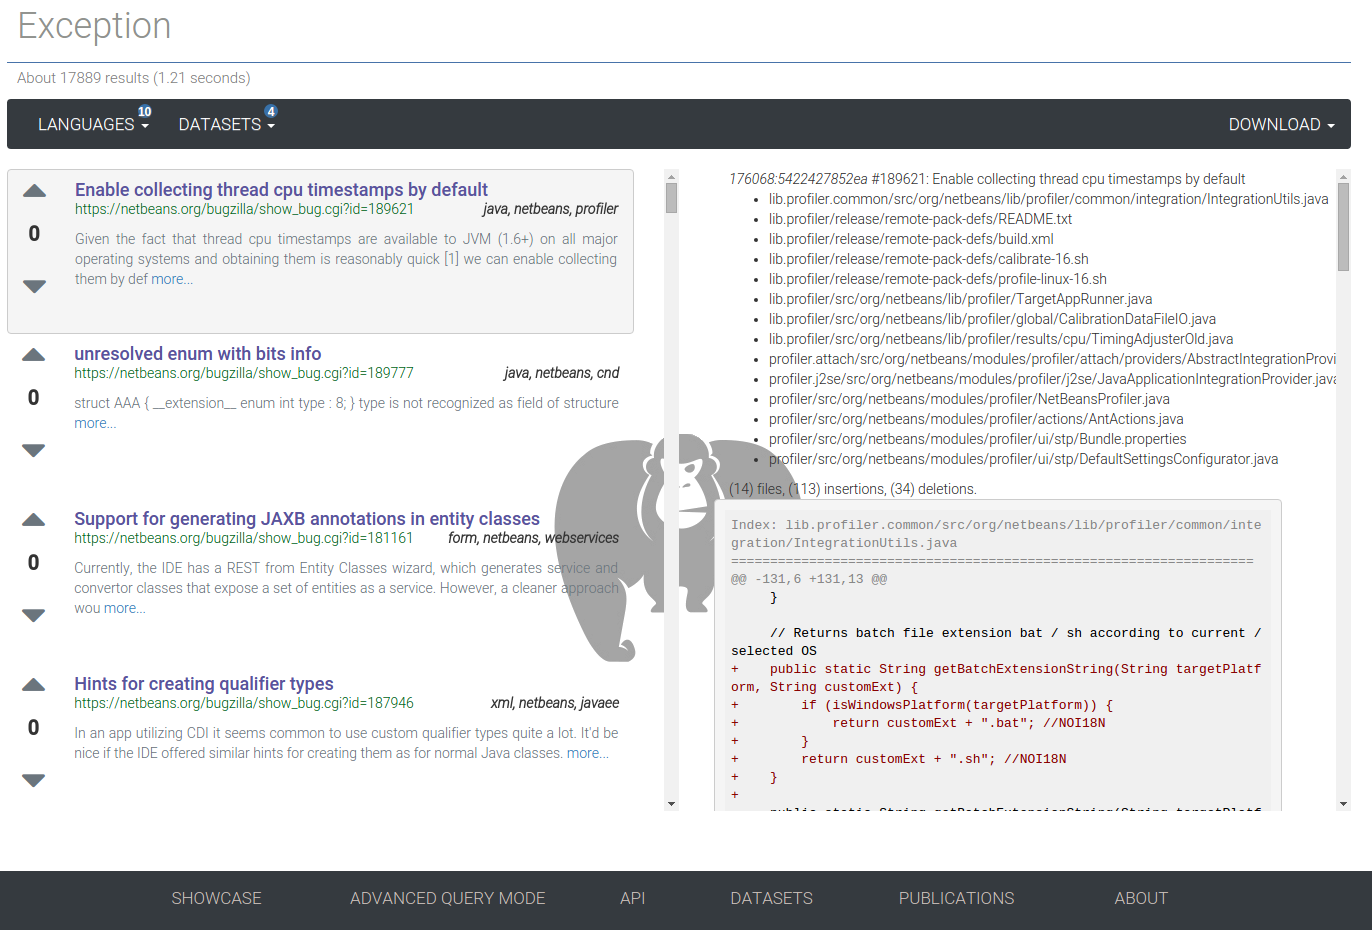
\includegraphics[scale=0.30]{media/bumper-live.png}
    \caption{Web Interface of BUMPER.
    \label{fig:bumper-ui}}
\end{figure}

\section{Empirical Validation}\label{empirical-validation}

Participants were asked to find a code snippet that can be slightly
modified in order to fix a bug using BUMPER and Google. The goal of this
preliminary study was to compare how fast a suitable fix can be found
using BUMPER and Google. We send our survey to 20 participants and
received eight responses (40\%) and asked them to report on their
experience in terms of the time taken to find a fix and the number of
Web pages that were browsed. Participants reported then when using
Google, it took, on average, 6.94 minutes by examining, in average, 7.57
online sources to find a fix. When using BUMPER, however, it only took
around 4.5 minutes. The participants only needed to use BUMPER and not
other websites. The feedback we received from the participants was very
encouraging. They mainly emphasized the ability of BUMPER to group many
repositories in one place, making the search for similar bugs/fixes
practical. We intend, in the future, to conduct a large scale (and more
formal) experiment with BUMPER for a thorough evaluation of its
effectiveness to help software developers in fixing bugs.

\section{Threats to Validity}\label{threats-to-validity}

The main threat to validity is our somewhat limited validation as we
only received eight responses. While the responses from this eight
developers are encouraging, a wider human study could invalidate them.

However, we see also BUMPER as an important tool for facilitating
research in the area of mining bug repositories. Studying software
repositories to gain insights into the quality of the code is a common
practice. This task requires time and skills in order to download and
link all the pieces of information needed for adequate mining. BUMPER
provides a straightforward interface to export bugs and their fixes into
CSV, XML and JSON. In short, BUMPER offers a framework that can be used
by software practitioners and researchers to analyse (efficiently) bugs
and their fixes without having to go from one repository to another,
worry about the way data is represented and saved, or create tools for
parsing and retrieving various data attributes. We hope that the
community contributes by adding more repositories to BUMPER. This way,
BUMPER can become a unified environment that can facilitate bug analysis
and mining tasks.

\section{Chapter Summary}\label{chapter-summary}

In this chapter, we presented a web-based infrastructure, called BUMPER
(BUg Metarepository for dEvelopers and Researchers). BUMPER allows
natural language searches in bugs reports, commit messages and source
code all together while supporting complex queries. Currently, BUMPER is
populated with 1,930 projects, more than 732,406 resolved/fixed and with
1,645,252 changesets from Eclipse, Gnome, Netbeans and the Apache
Software foundation. The speed of BUMPER allows developers to use it as
a way to leverage decades of history scattered over hundreds of software
projects in order to find existing solutions to their problems. There
exist tools such as Codemine {[}40{]} and Boa {[}50{]} that enable the
mining and reporting of code repositories. These tools, however, will
require the download of all the data and process the mining for each
installation. To the best of our knowledge, no attempt has been made
towards building unified and online datasets, from multiple sources,
where researchers and engineers can easily access all the information
related to a bug, or a fix in order to leverage decades of historical
information. Moreover, the feedback we received from the users of BUMPER
in a preliminary study shows that BUMPER holds real potential in
becoming a standard search engine for bugs and fixes in multiple
repositories.

This online dataset and its APIs were extensively used for the remaining
of this thesis.

\chapter{Preventing Code Clone Insertion At
Commit-Time}\label{preventing-code-clone-insertion-at-commit-time}

\section{Introduction}\label{introduction-2}

Code clones appear when developers reuse code with little to no
modification to the original code. Studies have shown that clones can
account for up to 50\% of code in a given software system {[}14, 48{]}.
Although developers often reuse code on purpose {[}98{]}, code cloning
is generally considered as a bad practice in software development
because clones may introduce bugs {[}89, 94, 118{]}.

In the last two decades, there have been many studies and tools that aim
at detecting clones. They can be grouped into two categories depending
on whether they operate locally on a developer's workstation (e.g.,
{[}170, 214{]}) or remotely on a server (e.g., {[}204, 211{]}).

Local clone detection approaches are typically implemented as IDE
plugins or external tools. IDE-based methods tend to issue many warnings
to developers that may interrupt their work, hence hindering their
productivity {[}103{]}. Developers may be reluctant to use external
tools unless they are involved in a major refactoring effort. These
tools cause overhead because of the context switching they provoke
{[}19, 160, 161{]}. This problem is somehow similar to the problem of
adopting bug identification tools. Studies have shown that these tools
are challenging to use because they do not integrate well with the
day-to-day workflow of developers {[}11, 58, 85, 113, 117{]}. The
problem with remote approaches is that the detection occurs too late in
the development process. Once the clones reach the central repository,
they can be pulled by other members of the development team, further
complicating the removal and management of clones.

In this chapter, we present PRECINCT (PREventing Clones INsertion at
Commit-Time) that focuses on preventing the insertion of clones at
commit-time (i.e., before they reach the central code repository).
PRECINCT is a trade-off between local and remote approaches. The
approach relies on the use of pre-commit hooks capabilities of modern
source code version control systems. A pre-commit hook is a process that
one can implement to receive the latest modification to the source code
done by a given developer just before the code reaches the central
repository. PRECINCT intercepts this modification and analyses its
content to see whether a suspicious clone has been introduced or not. A
flag is raised if a code fragment is suspected to be a clone of an
existing code segment. This said, only a fraction of the code is
analysed incrementally, making PRECINCT computationally efficient. In
other words, PRECINCT only operates on parts of the program that
changed.

To the best of our knowledge, PRECINCT is the first clone detection
technique that operates at commit-time. In this study, we focus on Type
3 clones as they are more challenging to detect {[}21, 93, 104{]}. Since
Type 3 clones include Type 1 and 2 clones, then these types could be
detected by PRECINCT as well. We evaluated the effectiveness of PRECINCT
on three systems, written in C and Java. The results show that PRECINCT
prevents Type 3 clones from reaching the final source code repository
with an average accuracy of 97.7\%.

\section{Approach}\label{approach-1}

\begin{figure*}
  \centering
  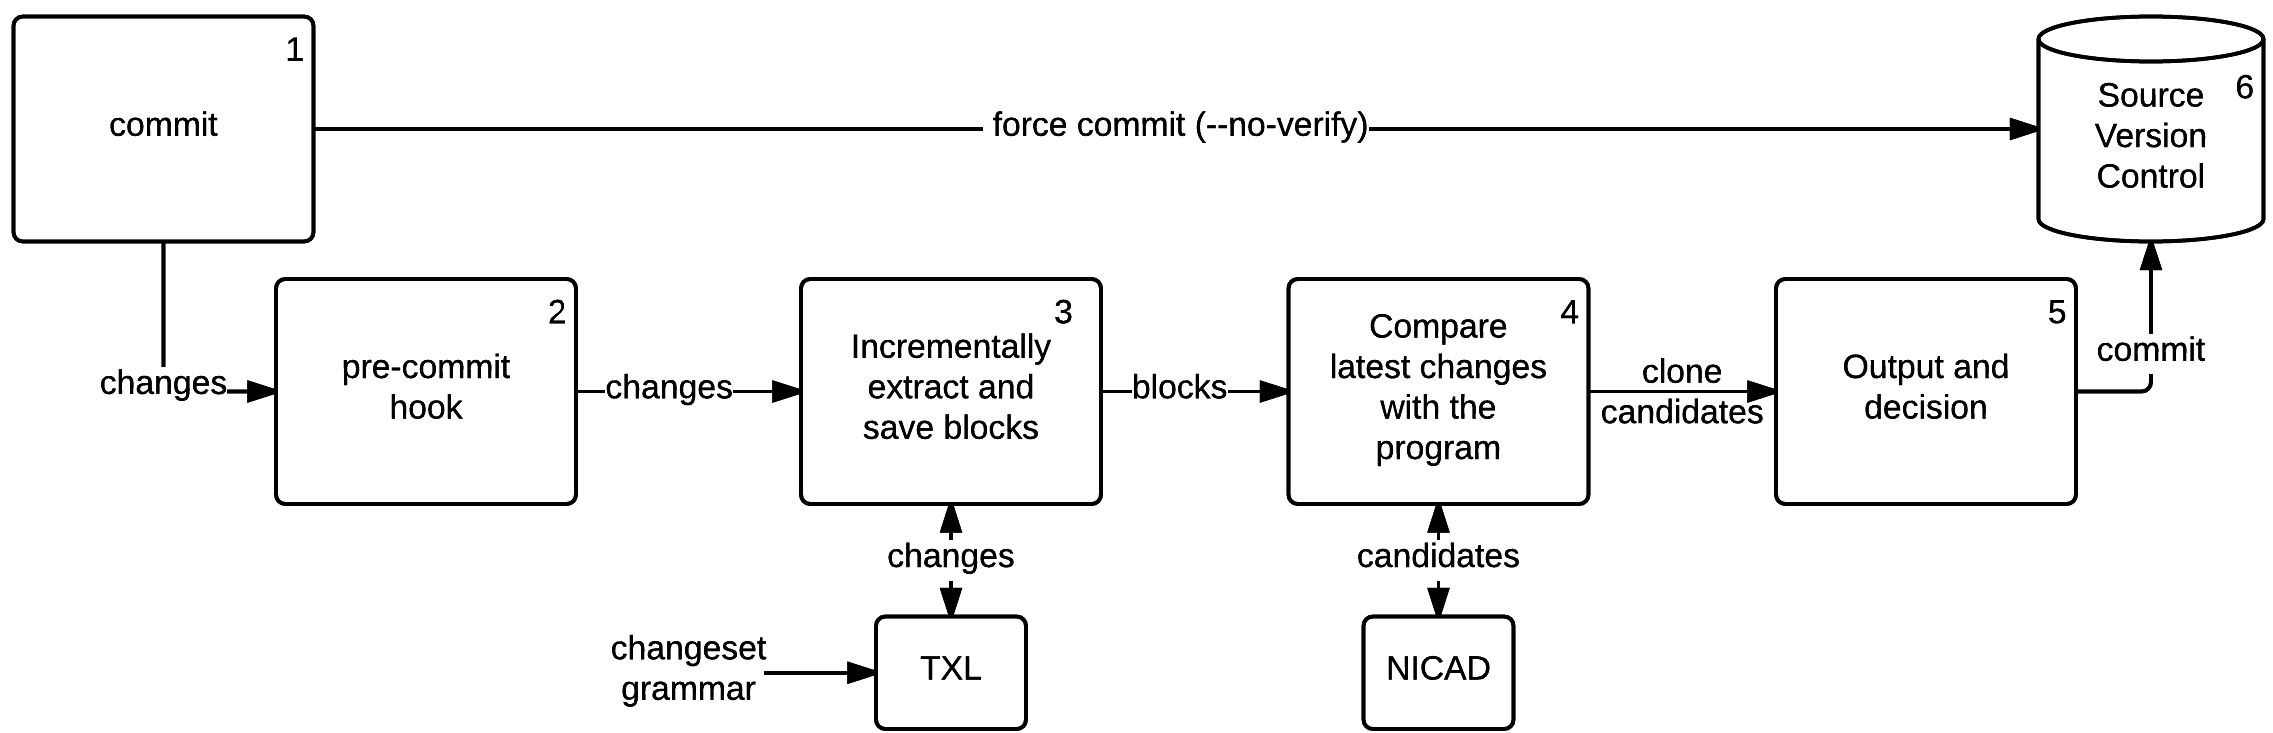
\includegraphics[width=0.95\textwidth]{media/chap5/approach.png}
  \caption{Overview of the PRECINCT approach.}
\end{figure*}

The PRECINCT approach is composed of six steps. The first and last steps
are typical steps that a developer would do when committing code. The
first step is the commit step where developers send their latest changes
to the central repository, and the last step is the reception of the
commit by the central repository. The second step is the pre-commit
hook, which kicks in as the first operation when one wants to commit.
The pre-commit hook has access to the changes regarding the files that
have been modified, more specifically, the lines that have been
modified. The modified lines of the files are sent to TXL {[}38{]} for
block extraction. Then, the blocks are compared to previously extracted
blocks to identify candidate clones using the comparison engine of NICAD
{[}39{]}. We chose NICAD engine because it has been shown to provide
high accuracy {[}39{]}. The tool is also readily available, easy to use,
customizable, and works with TXL. Note, however, that PRECINCT can also
work with other engines for comparing code fragments if need be.
Finally, the output of NICAD is further refined and presented to the
user for decision. These steps are discussed in more detail in the
following subsections.

\subsection{Commit}\label{commit}

In version control systems, a commit adds the latest changes made to the
source code to the repository, making these changes part of the head
revision of the repository. Commits in version control systems are kept
in the repository indefinitely. Thus, when other users do an update or a
checkout from the repository, they will receive the latest committed
version, unless they wish to retrieve a previous version of the source
code in the repository. Version control systems allow rolling back to
previous versions easily. Commits contain bite-sized units of work that
are potentially ready to be shared with the rest of the organisation
{[}148{]}.

\subsection{Pre-Commit Hook}\label{pre-commit-hook}

Hooks are custom scripts set to fire off when critical actions occur.
There are two groups of hooks: client-side and server-side. Client-side
hooks are triggered by operations such as committing and merging,
whereas server-side hooks run on network operations such as receiving
pushed commits. These hooks can be used for all sorts of reasons such as
compliance with coding rules or automatic run of unit test suites.

The pre-commit hook is run first, before one even types in a commit
message. It is used to inspect the snapshot that is about to be
committed. Depending on the exit status of the hook, the commit will be
aborted and not pushed to the central repository. Also, developers can
choose to ignore the pre-hook. In Git, for example, they will need to
use the command \lstinline!git commit –no-verify! instead of
\lstinline!git commit!. This can be useful in case of an urgent need for
fixing a bug where the code has to reach the central repository as
quickly as possible. Developers can do things like check for code style,
check for trailing white spaces (the default hook does exactly this), or
check for appropriate documentation on new methods.

PRECINCT is a set of bash scripts where the entry point of these scripts
lies in the pre-commit hooks. Pre-commit hooks are easy to create and
implement. Note that even though we use Git as the main version control
to present PRECINCT, the techniques presented in this paper are readily
applicable to other version control systems.

\subsection{Extract and Save Blocks}\label{extract-and-save-blocks}

A block is a set of consecutive lines of code that will be compared to
all other blocks to identify clones. To achieve this critical part of
PRECINCT, we rely on TXL {[}38{]}, which is a first-order functional
programming over linear term rewriting, developed by Cordy et al.
{[}38{]}. For TXL to work, one has to write a grammar describing the
syntax of the source language and the transformations needed. TXL has
three main phases: \emph{parse, transform}, \emph{unparse}. In the parse
phase, the grammar controls not only the input but also the output form.
The code sample below --- extracted from the official documentation ---
shows a grammar matching an \emph{if-then-else} statement in C with some
special keywords: {[}IN{]} (indent), {[}EX{]} (exdent) and {[}NL{]}
(newline) that will be used for the output form.

\begin{lstlisting}[language=bash]
define if_statement
  if ( [expr] ) [IN][NL]
    [statement] [EX]
    [opt else_statement]
end define

define else_statement
  else [IN][NL]
    [statement] [EX]
end define
\end{lstlisting}

Then, the \emph{transform} phase will, as the name suggests, apply
transformation rules that can, for example, normalize or abstract the
source code. Finally, the third phase of TXL called \emph{unparse},
unparses the transformed parsed input to output it. Also, TXL supports
what the creators call \emph{Agile Parsing} {[}46{]}, which allows
developers to redefine the rules of the grammar and, therefore, apply
different rules than the original ones.

PRECINCT takes advantage of that by redefining the blocks that should be
extracted for the purpose of clone comparison, leaving out the blocks
that are out of scope. More precisely, before each commit, we only
extract the blocks belonging to the modified parts of the source code.
Hence, we only process, in an incremental manner, the latest
modification of the source code instead of the source code as a whole.

We have selected TXL for several reasons. First, TXL is easy to install
and to integrate with the standard workflow of a developer. Second, it
was relatively easy to create a grammar that accepts commits as input.
This is because TXL is shipped with C, Java, C-sharp, Python and WSDL
grammars that define all the particularities of these languages, with
the ability to customize these grammars to accept changesets (chunks of
the modified source code that include the added, modified, and deleted
lines) instead of the whole code.

Algorithm \ref{alg:precinct-extract} presents an overview of the
``extract'' and ``save'' blocks operations of PRECINCT. This algorithm
receives as arguments, the changesets, the blocks that have been
previously extracted and a boolean named compare\_history. Then, from
Lines 1 to 9 lie the \(for\) loop that iterates over the changesets. For
each changeset (Line 1), we extract the blocks by calling the
\lstinline!extract_blocks(Changeset cs)! function. In this function, we
expand our changeset to the left and the right to have a complete block.

\begin{lstlisting}
@@ -315,36 +315,6 @@
int initprocesstree_sysdep
  (ProcessTree_T **reference) {
    mach_port_deallocate(mytask, task);
  }
}
- if (task_for_pid(mytask, pt[i].pid,
-  &task) == KERN_SUCCESS) {
-   mach_msg_type_number_t   count;
-   task_basic_info_data_t   taskinfo;
\end{lstlisting}

As depicted by above, changesets contain only the modified chunk of code
and not necessarily complete blocks. Indeed, we have a block from Line 2
to Line 6 and deleted lines from Line 7 to 10. However, in Line 7 we can
see the end of a block, but we do not have its beginning. Therefore, we
need to expand the changeset to the left to have syntactically correct
blocks. We do so by checking the block's beginning and ending (using \{
and \}) in C for example. Then, we send these expanded changesets to TXL
for block extraction and formalization.

For each extracted block, we check if the current block overrides
(replaces) a previous block (Line 4). In such a case, we delete the
previous block as it does not represent the current version of the
program anymore (Line 5). Also, we have an optional step in PRECINCT
defined in Line 4. The compare\_history is a condition to delete
overridden blocks.

We believe that deleted blocks have been removed for a good reason (bug,
default, removed features, \ldots{}) and if a newly inserted block
matches an old one, it could be worth knowing to improve the quality of
the system at hand.

In summary, this step receives the files and lines, modified by the
latest changes made by the developer and produces an up to date block
representation of the system at hand in an incremental way. The blocks
are analyzed in the next step to discover potential clones.

\begin{algorithm}
 \KwData{$Changeset[]$ changesets\;
 $Block[]$ prior\_blocks\;
 $Boolean$ compare\_history\;
 }
 \KwResult{Up to date blocks of the systems}
 \For{$i \leftarrow 0$ \KwTo$size\_of~changesets$}{
    Block[] blocks $\leftarrow$ $extract\_blocks(changesets)$\;
    \For{$j \leftarrow 0$ \KwTo$size\_of~blocks$}{
       \If{not $compare\_history$ AND $blocks[j]$ overrides one of $prior\_blocks$}{
          delete $prior\_block$\;
       }
       write $blocks[j]$\;
    }
 }

 \SetKwProg{myproc}{Function}{ $~extract\_blocks(Changeset~cs)$}{}
   \myproc{}{

   \uIf{$cs~is~unbalanced~right$}{$cs \leftarrow expand\_left(cs)$\;}

   \ElseIf{$cs~is~unbalanced~left$}{$cs \leftarrow expand\_right(cs)$\;}

   \nl\KwRet$txl\_extract\_blocks(cs)$\;
   }


 \caption{Overview of the Extract Blocks Operation\label{alg:precinct-extract}}
\end{algorithm}


\subsection{Compare Extracted Blocks}\label{compare-extracted-blocks}

To compare the extracted blocks and detect potential clones, we can only
resort to text-based techniques. This is because lexical and syntactic
analysis approaches (alternatives to text-based comparisons) would
require a complete program to work, a program that compiles. In the
relatively wide-range of tools and techniques that exist to detect
clones by considering code as text {[}48, 86, 87, 121, 123, 200{]}, we
selected NICAD as the main text-based method for comparing clones
{[}39{]} for several reasons. First, NICAD is built on top of TXL, which
we also used in the previous step. Second, NICAD can detect Type 1, 2
and 3 clones.

NICAD works in three phases: \emph{Extraction}, \emph{Comparison} and
\emph{Reporting}. During the \emph{Extraction} phase all potential
clones are identified, pretty-printed, and extracted. We do not use the
\emph{Extraction} phase of NICAD as it has been built to work on
programs that are syntactically correct, which is not the case for
changesets. We replaced NICAD's \emph{Extraction} phase with our own,
described in the previous section.

In the \emph{Comparison} phase, extracted blocks are transformed,
clustered and compared to find potential clones. Using TXL sub-programs,
blocks go through a process called pretty-printing where they are
stripped of formatting and comments. When code fragments are cloned,
some comments, indentation or spacing are changed according to the new
context where the new code is used. This pretty-printing process ensures
that all code will have the same spacing and formatting, which renders
the comparison of code fragments easier. Furthermore, in the
pretty-printing process, statements can be broken down into several
lines. Table \ref{tab:pretty-printing} {[}165{]} shows how this can
improve the accuracy of clone detection with three \lstinline!for!
statements, \lstinline!for (i=0; i<10; i++)!,
\lstinline!for (i=1; i<10; i++)! and \lstinline!for (j=2; j<100; j++)!.
The pretty-printing allows NICAD to detect Segments 1 and 2 as a clone
pair because only the initialization of \(i\) is changed. This specific
example would not have been marked as a clone by other tools we tested
such as Duploc {[}48{]}. In addition to the pretty-printing, the code
can be normalized and filtered to detect different classes of clones and
match user preferences.

\begin{table}[]
\centering
\caption{Pretty-Printing Example}
\label{tab:pretty-printing}
\resizebox{0.7\textwidth}{!}{%
\begin{tabular}{l|l|l|l|l|l}
Segment 1          & Segment 2          & Segment 3           & S1 \& S2 & S1 \& S3 & S2 \& S3 \\ \hline \hline
for (              & for (              & for (               & 1        & 1        & 1        \\
i = 0;             & i = 1;             & j = 2;              & 0        & 0        & 0        \\
i \textgreater 10; & i \textgreater 10; & j \textgreater 100; & 1        & 0        & 0        \\ 
i++)               & i++)               & j++)                & 1        & 0        & 0        \\ \hline \hline
\multicolumn{3}{c|}{Total Matches}                            & 3        & 1        & 1        \\ \hline
\multicolumn{3}{c|}{Total Mismatches}                         & 1        & 3        & 3
\end{tabular}
}
\end{table}


Finally, the extracted, pretty-printed, normalized and filtered blocks
are marked as potential clones using a Longest Common Subsequence (LCS)
algorithm {[}77{]}. Then, a percentage of unique statements can be
computed and, depending on a given threshold (see Section
\ref{sec:precinct-experimentations}), the blocks are marked as clones.

The last step of NICAD, which acts as our clone comparison engine, is
the \emph{reporting}. However, to prevent PRECINCT from outputting a
large amount of data (an issue that many clone detection techniques
face), we implemented our reporting system, which is also well embedded
with the workflow of developers. This reporting system is the subject of
the next section.

As a summary, this step receives potentially expanded and balanced
blocks from the extraction step. Then, the blocks are pretty-printed,
normalized, filtered and fed to an LCS algorithm to detect potential
clones. Moreover, the clone detection in PRECINCT is less intensive than
NICAD because we only compare the latest changes with the rest of the
program instead of comparing all the blocks with each other.

\subsection{Output and Decision}\label{output-and-decision}

In this final step, we report the result of the clone detection at
commit-time on the latest changes made by the developer. The process is
straightforward. Every change made by the developer goes through the
previous steps and is checked for the introduction of potential clones.
For each file that is suspected to contain a clone, one line is printed
to the command line with the following options: (I) Inspect, (D)
Disregard, (R) Remove from the commit. In comparison to this
straightforward and interactive output, NICAD outputs each and every
detail of the detection result such as the total number of potential
clones, the total number of lines, the total number of unique line text
chars, the total number of unique lines, and so on. We think that so
many details might make it hard for developers to react to these
results. A problem that was also raised by Johnson et al. {[}85{]} when
examining bug detection tools. Then the potential clones are stored in
XML files that can be viewed using an Internet browser or a text editor.

\begin{enumerate}
\def\labelenumi{(\Roman{enumi})}
\tightlist
\item
  Inspect will cause a diff-like visualization of the suspected clones
  while (D) disregard will simply ignore the finding. To integrate
  PRECINCT in the workflow of the developer, we also propose the remove
  option (R). This option will simply remove the suspected file from the
  commit that is about to be sent to the central repository.
\end{enumerate}

Figure \ref{fig:precinct-hook} shows an example of PRECINCT's output
when replaying commit \lstinline!710b6b4! of the Monit system. We think
that this output, at commit-time, is easy to work with for developers.
In addition, developers are used to interacting with their versioning
system in the command line. Consequently, we expect a gentle learning
curve.

\begin{figure}
  \centering
  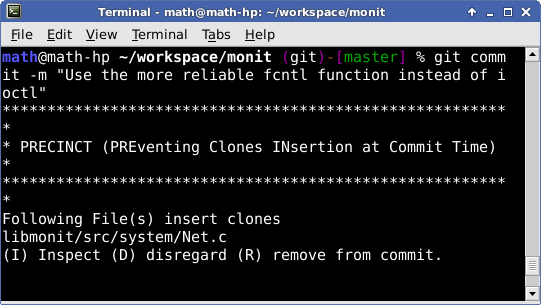
\includegraphics[width=\linewidth]{media/chap5/commit.png}
  \caption{PRECINCT output when replaying commit \texttt{710b6b4} of the Monit system used in the case study.\label{fig:precinct-hook}}
\end{figure}

\section{Experimental Setup}\label{experimental-setup-1}

Table \ref{tab:precinct-sut} shows the systems used in this study and
their characteristics in terms of the number files they contain and the
size in KLoC (Kilo Lines of Code). We also include the number of
revisions used for each system and the programming language in which the
system is written.

Monit is a small open source utility for managing and monitoring Unix
systems. Monit is used to conduct automatic maintenance and repair and
supports the ability to identify causal actions to detect errors. This
system is written in C and composed of 826 revisions, 264 files, and the
latest version has 107 KLoC. We have chosen Monit as a target system
because it was one of the systems NICAD was tested on.

JHotDraw is a Java GUI framework for technical and structured graphics.
It has been developed as a ``design exercise''. Its design is largely
based on the use of design patterns. JHotDraw is composed of 735
revisions, 1984 files, and the latest revision has 44 Kloc. It is
written in Java, and researchers often use it as a test bench. JHotDraw
was also used by NICAD's developers to evaluate their approach.

Dnsjava is a tool for implementing the DNS (Domain Name Service)
mechanisms in Java. This tool can be used for queries, zone transfers,
and dynamic updates. It is not as large as the other two, but it still
makes an interesting case subject because it has been well maintained
for the past decade. Consequently, it has a large number of revisions.
Also, this tool is used in many other popular tools such as Aspirin,
Muffin and Scarab. Dnsjava is composed of 1637 revisions, 233 files; the
latest revision contains 47 Kloc. We have chosen this system because we
are familiar with it as we used it before {[}137, 138{]}.

\begin{table}[]
\centering
\caption{List of Target Systems in Terms of Files and Kilo Line of Code (KLOC) at current version and Language}
\label{tab:precinct-sut}
\begin{tabular}{c|c|c|c|c}
SUT        & Revisions & Files & KLoC & Language \\ \hline\hline
Monit      & 826       & 264   & 107  & C        \\ \hline
Jhotdraw   & 735       & 1984  & 44   & Java     \\ \hline
dnsjava    & 1637      & 233   & 47   & Java     \\ \hline
\end{tabular}
\end{table}

As our approach relies on commit pre-hooks to detect possible clones
during the development process (more particularly at commit-time), we
had to find a way to \emph{replay} past commits. To do so, we
\emph{cloned} our test subjects, and then created a new branch called
\emph{PRECINCT\_EXT}. When created, this branch is reinitialized at the
initial state of the project (the first commit), and each commit can be
replayed as they have originally been. At each commit, we store the time
taken for PRECINCT to run as well as the number of detected clone pairs.
We also compute the size of the output in terms of the number of lines
of text output by our method. The aim is to reduce the output size to
help software developers interpret the results.

\begin{figure}
  \centering
  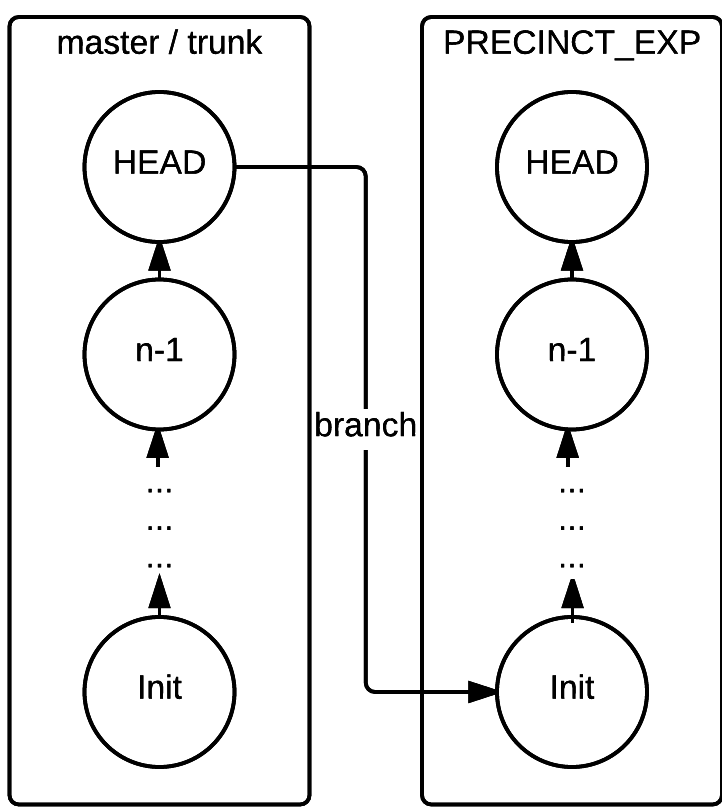
\includegraphics[width=0.5\linewidth]{media/chap5/branch.png}
  \caption{PRECINCT Branching.\label{fig:precinct-branching}}
\end{figure}

To validate the results obtained by PRECINCT, we needed to use a
reliable clone detection approach to extract clones from the target
systems and use these clones as a baseline for comparison. For this, we
turned to NICAD because of its popularity, high accuracy, and
availability {[}39{]}. This means, we run NICAD on the revisions of the
system to obtain the clones then we used NICAD clones as a baseline for
comparing the results achieved by PRECINCT.

It may appear strange that we are using NICAD to validate our approach,
knowing that our approach uses NICAD's code comparison engine. In fact,
what we are assessing here is the ability for PRECINCT to detect clones
at commit-time using changesets. The major part of PRECINCT is the
capacity to intercept code changes and build working code blocks that
are fed to a code fragment comparison engine (in our case NICAD's
engine). PRECINCT can be based on any other code comparison engine.

We show the result of detecting Type 3 clones with a maximum line
difference of 30\%. As discussed in the introductory section, we chose
to report on Type 3 clones because they are more challenging to detect
than Type 1 and 2. PRECINCT detects Type 1 and 2 too, so does NICAD. For
the time being, PRECINCT is not designed to detect Type 4 clones. These
clones use different implementations. Detecting Type 4 clones is part of
future work.

We assess the performance of PRECINCT in terms of precision, recall, and
F\(_{1}\)-measure by using NICAD's results as ground truth. They are
computed using TP (true positives), FP (false positives), FN (false
negatives), which are defined as follows:

\begin{itemize}
\tightlist
\item
  TP: is the number of clones that were properly detected by PRECINCT
  (again, using NICAD's results as baseline)
\item
  FP: is the number of non-clones that were classified by PRECINCT as
  clones
\item
  FN: is the number of clones that were not detected by PRECINCT
\item
  Precision: TP / (TP + FP)
\item
  Recall: TP / (TP + FN)
\item
  F1-measure: 2.(precision.recall)/(precision+recall)
\end{itemize}

\section{\texorpdfstring{Empirical Validation
\label{sec:precinct-experimentations}}{Empirical Validation }}\label{empirical-validation-1}

\begin {figure*}%[!hbtp]
\centering
\begin{tikzpicture}
    \begin{axis}[
      scale only axis, % The height and width argument only apply to the actual axis
    height=5cm,
    width=0.9\textwidth,
    grid = both,
    minor tick num=1,
    xlabel={Revisions},
    ylabel={Clones},
    xmin=0]
    \addplot table [smooth,red,mark=none,x=revision,y=clones,col sep=comma] {data/chap5/monit.csv};
    \addlegendentry{NICAD Detection}

    \addplot table [smooth,blue,mark=none,x=revision,y=detected,col sep=comma] {data/chap5/monit.csv};
    \addlegendentry{PRECINCT Detection}

    \addplot table [smooth,red,mark=none,x=revision,y=prevented,col sep=comma] {data/chap5/monit.csv};
    \addlegendentry{Remaining Clones}

    \end{axis}
    \end{tikzpicture}
    \caption{Monit clone detection over revisions\label{fig:precinct-r1}}
\end{figure*}

\begin {figure*}%[!hbtp]
\centering
\begin{tikzpicture}
    \begin{axis}[
      scale only axis, % The height and width argument only apply to the actual axis
    height=5cm,
    width=0.9\textwidth,
    grid = both,
    minor tick num=1,
    xlabel={Revisions},
    ylabel={Clones},
    xmin=0]
  \addplot table [smooth,red,mark=none,x=revision,y=clones,col sep=comma] {data/chap5/jhotdraw.csv};
      \addlegendentry{NICAD Detection}

    \addplot table [smooth,green,mark=none,x=revision,y=detected,col sep=comma] {data/chap5/jhotdraw.csv};
    \addlegendentry{PRECINCT Detection}

    \addplot table [smooth,red,mark=none,x=revision,y=prevented,col sep=comma] {data/chap5/jhotdraw.csv};
    \addlegendentry{Remaining Clones}

    \end{axis}
    \end{tikzpicture}
    \caption{JHotDraw clone detection over revisions\label{fig:precinct-r2}}
\end{figure*}

\begin {figure*}%[!hbtp]
\centering
\begin{tikzpicture}
    \begin{axis}[
      scale only axis, % The height and width argument only apply to the actual axis
    height=5cm,
    width=0.9\textwidth,
    grid = both,
    minor tick num=1,
    xlabel={Revisions},
    ylabel={Clones},
    xmin=0]
  \addplot table [smooth,red,mark=none,x=revision,y=clones,col sep=comma] {data/chap5/dnsjava.csv};
    \addlegendentry{NICAD Detection}

    \addplot table [smooth,green,mark=none,x=revision,y=detected,col sep=comma] {data/chap5/dnsjava.csv};
    \addlegendentry{PRECINCT Detection}

    \addplot table [smooth,red,mark=none,x=revision,y=prevented,col sep=comma] {data/chap5/dnsjava.csv};
    \addlegendentry{Remaining Clones}

    \end{axis}
    \end{tikzpicture}
    \caption{Dnsjava clone detection over revisions\label{fig:precinct-r3}}
\end{figure*}


Figures \ref{fig:precinct-r1}, \ref{fig:precinct-r2},
\ref{fig:precinct-r3} show the results of our study in terms of clone
pairs that are detected per revision for our three subject systems:
Monit, JHotDraw and Dnsjava. We used as a baseline for comparison the
clone pairs detected by NICAD. The blue line shows the clone detection
performed by NICAD. The red line shows the clone pairs detected by
PRECINCT. The brown line shows the clone pairs that have been missed by
PRECINCT. As we can quickly see, the blue and red lines almost overlap,
which indicates a good accuracy of the PRECINCT approach.

\begin{table*}[]
\centering
\caption{Overview of PRECINCT's results in terms of precision, recall, F$_{1}$-measure, execution time and output reduction.}
\label{tab:result-precinct}
\resizebox{\textwidth}{!}{%
\begin{tabular}{c|c|c|c|c|c||c|c}
         &  Detected & Precision & Recall & F1-measure & \begin{tabular}[c]{@{}c@{}}NICAD's Average\\ Execution Time\end{tabular} & \begin{tabular}[c]{@{}c@{}}PRECINCT's Average \\ Execution Time\end{tabular} & \begin{tabular}[c]{@{}c@{}}Overall \\ Output Reduction\end{tabular} \\ \hline\hline
Monit      & 123      & 96.1\%    & 100\%  & 98\%       & 2.2s                                                                     & 0.9s                                                                         & 88.3\%                                                              \\ \hline
JHotDraw   & 6490     & 98.3\%    & 100\%  & 99.1\%     & 5.1s                                                                     & 1.7s                                                                         & 70.1\%                                                              \\ \hline
DnsJava    & 226      & 82.8\%    & 100\%  & 90.6\%     & 1.8s                                                                     & 1.1s                                                                         & 88.6\%                                                              \\ \hline\hline
Total      & 6839     & 97.7\%    & 100\%  & 98.8\%     & 3s                                                                       & 1.2s                                                                         & 83.4\%                                                              \\ \hline
\end{tabular}
}
\end{table*}


Table \ref{tab:result-precinct} summarizes PRECINCT's results in terms
of precision, recall, F\(_{1}\)-measure, execution time and output
reduction compared to NICAD for our three subject systems: Monit,
JHotDraw, and Dnsjava. The first version of Monit contains 85 clone
pairs, and this number stays stable until Revision 100. From Revision
100 to 472 the detected clone pairs vary between 68 and 88 before
reaching 219 at Revision 473. The number of clone pairs goes down to 122
at Revision 491 and increases to 128 in the last revision. PRECINCT was
able to detect 96.1\% (123/128) of the clone pairs that are detected by
NICAD with a 100\% recall. It took in average around 1 second for
PRECINCT to execute on a Debian 8 system with Intel(R) Core(TM) i5-2400
CPU @ 3.10GHz, 8Gb of DDR3 memory. It is also worth mentioning that the
computer we used is equipped with SSD (Solid State Drive). This impacts
the running time as clone detection is a file intensive operation.
Finally, the PRECINCT was able to output up to 88.3\% fewer lines than
NICAD.

JHotDraw starts with 196 clone pairs at Revision 1 and reaches a pick of
2048 at Revision 180. The number of clones continues to go up until
Revisions 685 and 686 where the number of pairs is 1229 before picking
at 6538 from Revisions 687 to 721. PRECINCT was able to detect 98.3\% of
the clone pairs detected by NICAD (6490/6599) with 100\% recall while
executing on average in 1.7 seconds (compared to 5.1 seconds for NICAD).
With JHotDraw, we can see the advantages of incremental approaches.
Indeed, the execution time of PRECINCT is loosely impacted by the number
of files inside the system as the blocks are constructed incrementally.
Also, we only compare the latest change to the remaining of the program
and not all the blocks to each other as NICAD. We also were able to
reduce by 70.1\% the number of lines outputted.

Finally, for Dnsjava, the number of clone pairs starts high with 258
clones and goes down until Revision 70 where it reaches 165. Another
quick drop is observed at Revision 239 where we found only 25 clone
pairs. The number of clone pairs stays stable until Revision 1030 where
it reaches 273. PRECINCT was able to detect 82.8\% of the clone pairs
detected by NICAD (226/273) with 100\% recall while executing on average
in 1.1 seconds while NICAD took 3 seconds in average. PRECINCT outputs
83.4\% fewer lines than NICAD.

Overall, PRECINCT prevented 97.7\% of the 7000 clones (in all systems)
to reach the central source code repository while executing more than
twice as fast as NICAD (1.2 seconds compared to 3 seconds in average)
and reducing the output in terms of lines of text output to the
developers by 83.4\% in average. Note here that we have not evaluated
the quality of the output of PRECINCT compared to NICAD's output. We
need to conduct user studies for this. We are, however, confident, based
on our experience trying many clone detection tools, that a simpler and
a more interactive way to present the results of a clone detection tool
is warranted. PRECINCT aims to do just that.

The difference in execution time between NICAD and PRECINCT stems from
the fact that, unlike PRECINCT, NICAD is not an incremental approach.
For each revision, NICAD has to extract all the code blocks and then
compares all the pairs with each other. On the other hand, PRECINCT only
extracts blocks when they are modified and only compares what has been
changed with the rest of the program.

The difference in precision between NICAD and PRECINCT (2.3\%) can be
explained by the fact that sometimes developers commit code that does
not compile. Such commits will still count as a revision, but TXL fails
to extract blocks that do not comply with the target language syntax.
While NICAD also fails in such a case, the disadvantage of PRECINCT
comes from the fact that the failed block is saved and used as a
reference until it is changed by a correct one in another commit.

\section{Threats to Validity}\label{threats-to-validity-1}

The selection of target systems is one of the common threats to validity
for approaches aiming to improve the analysis of software systems. It is
possible that the selected programs share common properties that we are
not aware of and therefore, invalidate our results. However, the systems
analyzed by PRECINCT are the same as the ones used in similar studies.
Moreover, the systems vary in terms of purpose, size, and history.

Also, we see a threat to validity that stems from the fact that we only
used open source systems. The results may not be generalizable to
industrial systems. We intend to undertake these studies in future work.

The programs we used in this study are all based on the Java, C, and
Python programming languages. This can limit the generalization of the
results. However, similar to Java, C, Python, if one writes a TXL
grammar for a new language --- which can be relatively hard work ---
then PRECINCT can work since PRECINCT relies on TXL.

Finally, we use NICAD as the code comparison engine. The accuracy of
NICAD affects the accuracy of PRECINCT. This said, since NICAD has been
tested on large systems, we are confident that it is a suitable engine
for comparing code using TXL. Also, there is nothing that prevents us
from using other code comparisons engines, if need be.

In conclusion, internal and external validity have both been minimized
by choosing a set of three different systems, using input data that can
be found in any programming languages and version systems (commit and
changesets).

\section{Chapter Summary}\label{chapter-summary-1}

In this chapter, we presented PRECINCT (PREventing Clones INsertion at
Commit-Time), an incremental approach for preventing clone insertion at
commit-time that combines efficient block extraction and clone
detection. The approach is meant to integrate well with the workflow of
developers. PRECINCT takes advantage of TXL and NICAD to create a clone
detection tool that runs automatically before each commit in an average
time of 1.2 seconds with an average 97.7\% precision and 100\% recall
(when using NICAD's results as a baseline).

Our approach is an efficient trade-off between local and remote
approaches for clone detection, and as such, we believe that it
addresses major factors that contribute to the slow adoption of clone
detection tools. PRECINCT achieves similar performance than remote
approaches, which rely on more computational power, without delaying the
detection results in asynchronous email notifications. Moreover, we
believe that operating at commit-time makes PRECINCT more appealing to
developers. Using PRECINCT, developers do not have to cope with many
warnings and the problem of context-switching, which are the main
limitations of IDE-based methods and the use of external tools. Finally,
our approach can reduce the number of lines output by a traditional
clone detection tool such as NICAD by 83.4\% while keeping all the
necessary information that would allow developers to decide whether the
detected clone is, in fact, a clone.

In the remaining of this thesis, we build upon BUMPER and PRECINCT to
detect risky commit and propose solutions to improve code at
commit-time.

\chapter{Preventing Bug Insertion Using Clone Detection At
Commit-Time}\label{preventing-bug-insertion-using-clone-detection-at-commit-time}

\section{Introduction}\label{introduction-3}

Research in software maintenance has evolved over the year to include
areas like mining bug repositories, bug analytic, and bug prevention and
reproduction. The ultimate goal is to develop better techniques and
tools to help software developers detect, correct, and prevent bugs
effectively and efficiently.

One particular (and growing) line of research focuses on the problem of
preventing the introduction of bugs by detecting risky commits
(preferably before the commits reach the central repository). Recent
approaches (e.g., {[}119, 132{]}) rely on training models based on code
and process metrics (e.g., code complexity, experience of the
developers, etc.) that are used to classify new commits as risky or not.
Metrics, however, may vary from one project to another, hindering the
reuse of these models. Consequently, these techniques tend to operate
within single projects only, despite the fact that many large projects
share dependencies, such as the reuse of common libraries. This makes
them potentially vulnerable to similar faults. A solution to a bug
provided by the developers of one project may help fix a bug that occurs
in another (and dependent) project. Moreover, as noted by Lewis \emph{et
al.} {[}117{]} and Johnson \emph{et al.} {[}85{]}, techniques based
solely on metrics are perceived by developers as black box solutions
because they do not provide any insights on the causes of the risky
commits or ways for improving them. As a result, developers are less
likely to trust the output of these tools.

In this chapter, we present a novel bug prevention approach at
commit-time, called BIANCA (Bug Insertion ANticipation by Clone Analysis
at commit time). BIANCA does not use metrics to assess whether or not an
incoming commit is risky. Instead, it relies on code clone detection
techniques by extracting code blocks from incoming commits and comparing
them to those of known defect-introducing commits.

One particular aspect of BIANCA is its ability to detect risky commits
not only by comparing them to commits of a single project but also to
those belonging to other projects that share common dependencies. This
is important because complex software systems are not designed
monolithically. They have dependencies that make them vulnerable to
similar faults. For example, Apache BatchEE {[}183{]} and GraphWalker
{[}63{]} both depend on JUNG (Java Universal Network/Graph Framework)
{[}88{]}. BatchEE provides an implementation of the jsr-352 (Batch
Applications for the Java Platform) specification {[}35{]} while
GraphWalker is an open source model-based testing tool for test
automation. These two systems are designed for different purposes.
BatchEE is used to do batch processing in Java, whereas GraphWalker is
used to design unit tests using a graph representation of the code.
Nevertheless, because both Apache BatchEE and GraphWalker rely on JUNG,
the developers of these projects made similar mistakes when building
upon JUNG. Issue \#69 and \#44 from Apache BatchEE and Graphwaler,
respectively, indicate that the developers of these projects made
similar mistakes when using the graph visualization component of JUNG.
To detect \emph{risky} commits across projects, BIANCA resorts to
project dependency analysis. Note that we do not detect only the bugs
resulting from library usage but rather leverage the fact that if two
systems use the same libraries, then they are likely vulnerable to the
same flaws.

Another advantage of BIANCA is that it uses commits that are used to fix
previous defect-introducing commits to guide the developers on how to
improve risky commits. This way, BIANCA goes one step further than
existing techniques by providing developers with a potential fix for
their risky commits.

We validated the performance of BIANCA on 42 open source projects,
obtained from Github. The examined projects vary in size, domain and
popularity. Our findings indicate that BIANCA is able to flag risky
commits with an average precision, recall and F-measure of 90.75\%,
37.15\% and 52.72\%, respectively. Although the performance of BIANCA
seems modest, it is important to ground these results with the fact that
BIANCA outperforms a baseline model by 19.48\% (mainly due to the data
imbalance, i.e., most commits are not defect-inducing). Moreover, we
found that only 8.6\% of the risky commits detected by BIANCA match
other commits from the same project. This finding stresses the fact that
relationships across projects should be taken into consideration for
effective prevention of risky commits.

\section{Approach}\label{approach-2}

Figures \ref{fig:bianca1}, \ref{fig:bianca3} and \ref{fig:bianca2} show
an overview of the BIANCA approach, which consists of two parallel
processes.

In the first process (Figures \ref{fig:bianca1} and \ref{fig:bianca3}),
BIANCA manages events happening on project tracking systems to extract
defect-introducing commits and commits that provided the fixes. For
simplicity, in the rest of this paper, we refer to commits that are used
to fix defects as \emph{fix-commits}. We use the term
\emph{defect-commit} to mean a commit that introduces a defect. In the
second phase, BIANCA analyses the developer's new commits before they
reach the central repository to detect potential risky commits (commits
that may introduce bugs).

\begin{figure*}
  \centering
    \includegraphics[width=\textwidth]{media/chap6/fix-approach.png}
    \caption{Managing events happening on project tracking systems to extract defect-introducing commits and commits that provided the fixes\label{fig:bianca1}}
\end{figure*}

\begin{figure*}
  \centering
    \includegraphics[width=0.7\textwidth]{media/chap6/cluster-approach}
    \caption{Clustering by dependency\label{fig:bianca3}}
\end{figure*}

\begin{figure*}
  \centering
    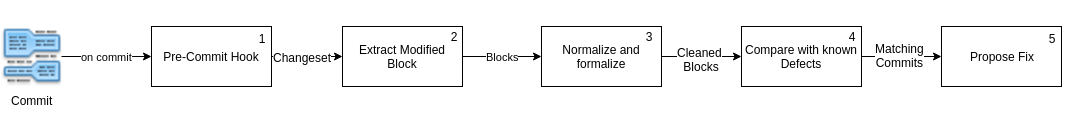
\includegraphics[width=\textwidth]{media/chap6/detect-approach}
    \caption{Classifying incoming commits and proposing fixes\label{fig:bianca2}}
\end{figure*}



The project tracking component of BIANCA listens to bug (or issue)
closing events of major open-source projects (currently, BIANCA is
tested with 42 large projects). These projects share many dependencies.
Projects can depend on each other or common external tools and
libraries. We perform project dependency analysis to identify groups of
highly-coupled projects.

In the second process (Figure \ref{fig:bianca2}), BIANCA identifies
risky commits within each group to increase the chances of finding risky
commits caused by project dependencies. For each project group, we
extract code blocks from defect-commits and fix-commits. The extracted
code blocks are saved in a database that is used to identify risky
commits before they reach the central repository. For each match between
a risky commit and a \emph{defect-commit}, we pull out from the database
the corresponding \emph{fix-commit} and present it to the developer as a
potential way to improve the commit content. These phases are discussed
in more detail in the upcoming subsections.

\subsection{Clustering Project Repositories}\label{sec:clustering}

We cluster projects according to their dependencies. The rationale is
that projects that share dependencies are most likely to contain defects
caused by misuse of these dependencies. In this step, the project
dependencies are analysed and saved into a single NoSQL graph database
as shown in Figure \ref{fig:bianca3}. Graph databases use graph
structures as a way to store and query information. In our case, a node
corresponds to a project that is connected to other projects on which it
depends. Project dependencies can be automatically retrieved if projects
use a dependency manager such as Maven.

Figure \ref{fig:network-sample} shows a simplified view of a dependency
graph for a project named \texttt{com.badlogicgames.gdx}. As we can see,
\texttt{com.badlogicgames.gdx} depends on projects owned by the same
organization (i.e., badlogicgames) and other organizations such as
Google, Apple, and Github.

\begin{figure*}
  \centering
    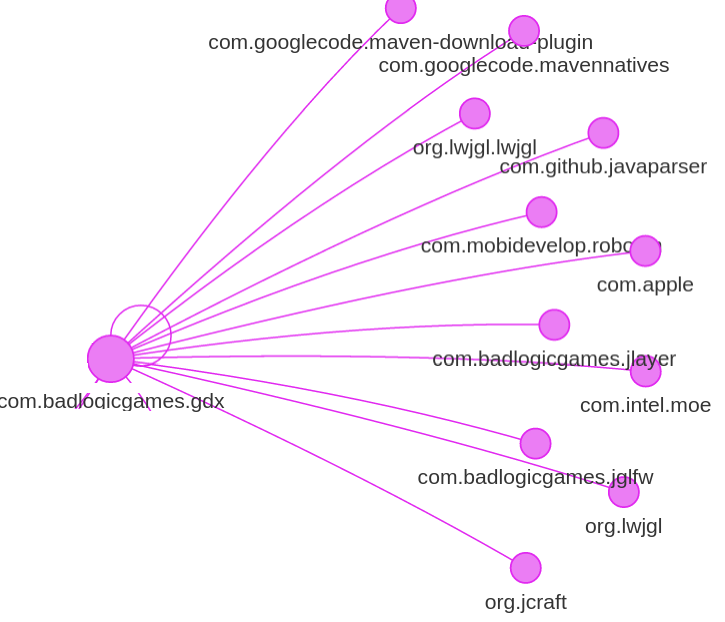
\includegraphics[width=0.60\textwidth]{media/chap6/network-sample.png}
    \caption{Simplified Dependency Graph for \texttt{com.badlogicgames.gdx}\label{fig:network-sample}}
\end{figure*}

Once the project dependency graph is extracted, we use a clustering
algorithm to partition the graph. To this end, we choose the
Girvan--Newman algorithm {[}61, 143{]}, used to detect communities by
progressively removing edges from the original network. Instead of
trying to construct a measure that identifies the edges that are the
most central to communities, the Girvan--Newman algorithm focuses on
edges that are most likely ``between'' communities. This algorithm is
very effective at discovering community structure in both
computer-generated and real-world network data {[}143{]}. Other
clustering algorithms can also be used.

\subsection{Building a Database of Code Blocks of Defect-Commits and
Fix-Commits}\label{sec:offline}

To build our database of code blocks that are related to defect-commits
and fix-commits, we first need to identify the respective commits. Then,
we extract the relevant blocks of code from the commits.

\textbf{Extracting Commits:} BIANCA listens to bug (or issue) closing
events happening in the project tracking system. Every time an issue is
closed, BIANCA retrieves the commit that was used to fix the issue (the
fix-commit) as well as the one that introduced the defect (the
defect-commit). Retrieving fix-commits, however, is known to be a
challenging task {[}202{]}. This is because the link between the project
tracking system and the code version control system is not always
explicit. In an ideal situation, developers would add a reference to the
issue they work on inside the description of the commit. However, this
good practice is not always followed. To link fix-commits and their
related issues, we turn to a modified version of the back-end of
commit-guru {[}163{]}. Commit-guru is a tool, developed by Rosen
\emph{et al.} {[}163{]} to detect \emph{risky commits}. In order to
identify risky commits, Commit-guru builds a statistical model using
change metrics (i.e., amount of lines added, amount of lines deleted,
amount of files modified, etc.) from past commits known to have
introduced defects in the past.

Commit-guru's back-end has three major components: ingestion, analysis,
and prediction. We reuse the ingestion and the analysis part for BIANCA.
The ingestion component is responsible for ingesting (i.e., downloading)
a given repository. Once the repository is entirely downloaded on a
local server, each commit is analysed. Commits are classified using the
list of keywords proposed by Hindle \emph{et al.} {[}73{]}. Commit-guru
implements the SZZ algorithm {[}100{]} to detect risky changes, where it
performs the SCM blame/annotate function on all the modified lines of
code for their corresponding files on the fix-commit's parents. This
returns the commits that previously modified these lines of code and are
flagged as the defect introducing commits (i.e., the defect-commits).
Prior work showed that commit-guru is effective in identifying
defect-commits and their corresponding fixing commits {[}91{]} and the
SZZ algorithm, used by commit-guru, is shown to be effective in
detecting risky commits {[}91, 163{]}. Note that we could use a simpler
and more established approach such as Relink {[}202{]} to link the
commits to their issues and re-implement the classification proposed by
Hindle \emph{et al.} {[}73{]} on top of it. However, commit-guru has the
advantage of being open-source, making it possible to modify it to fit
our needs by fine-tuning its performance.

\textbf{Extracting Code Blocks:} To extract code blocks from fix-commits
and defect-commits, we rely on PRECINCT which has been presented in the
previous chapter.

\subsection{Analysing New Commits Using Pre-Commit
Hooks}\label{sec:online}

Each time a developer makes a commit, BIANCA intercepts it using a
pre-commit hook extracts the corresponding code block (in a similar way
as in the previous phase), and compares it to the code blocks of
historical defect-commits. If there is a match, then the new commit is
deemed to be risky. A threshold \(\alpha\) is used to assess the extent
beyond which two commits are considered similar. The setting of
\(\alpha\) is discussed in the case study section.

BIANCA is based on a set of bash and python scripts, and the entry point
of these scripts lies in a pre-commit hook. These scripts intercept the
commit and extract the corresponding code blocks.

We use pre-commit hook, which kicks in as the first operation when one
wants to commit. The pre-commit hook has access to the changes regarding
the files that have been modified, more specifically, the lines that
have been modified. The modified lines of the files are sent to TXL with
our special grammar and algorithm (Algorithm \ref{alg:precinct-extract}
presented in the previous chapter.

Then, the blocks are compared to previously extracted blocks known to
introduce a defect using the comparison engine of NICAD {[}39{]}.

To compare the extracted blocks to the ones in the database, we use a
similar strategy as the one presented in the previous chapter.

Another important aspect of the design of BIANCA is the ability to
provide guidance to developers on how to improve risky commits. We
achieve this by extracting from the database the fix-commit
corresponding to the matching defect-commit and present it to the
developer. We believe that this makes BIANCA a practical approach for
the developers as they will know why a given modification has been
reported as risky in terms of code; this is something that is not
supported by techniques based on statistical models (e.g., {[}91,
163{]}).\\
A tool that supports BIANCA should have enough flexibility to allow
developers to enable or disable the recommendations made by BIANCA.
Furthermore, because BIANCA acts before the commit reach the central
repository, it prevents unfortunate pulls of defects by other members of
the organization.

\section{Experimental Setup}\label{experimental-setup-2}

In this section, we present the setup of our case study in terms of
repository selection, dependency analysis, comparison process and
evaluation measures.

\subsection{Project Repository Selection}\label{sec:rep}

To select the projects used to evaluate our approach, we followed three
simple criteria. First, the projects need to be in Java and use Maven to
manage dependencies. This way, we can automatically extract the
dependencies and perform the clustering of projects. The second
criterion is to have projects that enjoy a large community support and
interest. We selected projects that have at least 2000 followers.
Finally, the projects must have a public issue repository to be able to
mine their past issues and the fixes. We queried Github with these
criteria and retrieved 42 projects (see Table \ref{tab:results} for the
list of projects), including those from some of major open-source
contributors such as Alibaba, Apache Software Foundation, Eclipse,
Facebook, Google and Square.

\subsection{Project Dependency Analysis}\label{sec:dependencies}

Figure \ref{fig:dep-graph} shows the project dependency graph. The
dependency graph is composed of 592 nodes divided into five clusters
shown in yellow, red, green, purple and blue. The size of the nodes in
Figure \ref{fig:dep-graph} is proportional to the number of connections
from and to the other nodes.

\begin{figure*}
  \centering
    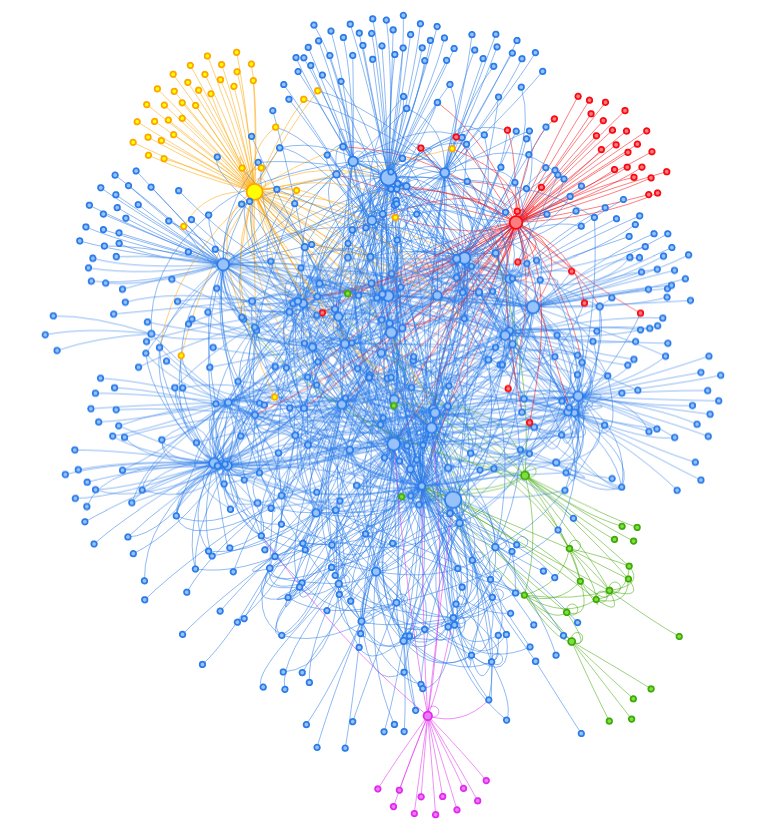
\includegraphics[width=0.80\textwidth]{media/chap6/network.png}
    \caption{Dependency Graph\label{fig:dep-graph-bianca}}
\end{figure*}

As shown in Figure \ref{fig:dep-graph}, these Github projects are very
much interconnected. On average, the projects composing our dataset have
77 dependencies. Among the 77 dependencies, on average, 62 dependencies
are shared with at least one other project from our dataset.

Table \ref{tab:communities} shows the result of the Girvan--Newman
clustering algorithm in terms of centroids and betweenness. Storm
dominates the blue cluster from The Apache Software Foundation. Storm is
a distributed real-time computation system. Druid by Alibaba, the
e-commerce company that provides consumer-to-consumer,
business-to-consumer and business-to-business sales services via web
portals, dominates the yellow cluster. In recent years, Alibaba has
become an active member of the open-source community by making some of
its projects publicly available. The red cluster has Hadoop by the
Apache Software Foundation as its centroid. Hadoop is an open-source
software framework for distributed storage and distributed processing of
very large datasets on computer clusters built from commodity hardware.
The Persistence project of OpenHab dominates the green cluster. OpenHab
proposes home automation solutions, and the \emph{persistence} project
is their data access layer. Finally, the purple cluster is dominated by
Libdx by Badlogicgames, which is a cross-platform framework for game
development.

A review of each cluster shows that this partitioning divides projects
in terms of high-level functionalities. For example, the blue cluster is
almost entirely composed of projects from the Apache Software
Foundation. Projects from the Apache Software Foundation tend to build
on top of one another. We also have the red cluster for Hadoop, which is
by itself an ecosystem inside the Apache Software Foundation. Finally,
we obtained a cluster for e-commerce applications (yellow), real-time
network application for home automation (green), and game development
(purple).


\begin{table*}[]
\centering
\caption{Communities in terms of ID, Color code, Centroids, Betweenness and number of members}
\label{tab:communities}
\begin{tabular}{llllcc}
\hline
\#ID               & Community             & Centroids        & Betweenness & \# Members        \\ \hline
1                  & Blue                  & Storm &           24,525 &    479                                      \\ \hline
2                  & Yellow                & Alibaba          & 24,400      & 42                                      \\ \hline
3                  & Red                   & Hadoop           & 16,709      & 37                                      \\ \hline
4                  & Green                 & Openhab          & 3,504       & 22                                      \\ \hline
5                  & Purple                & Libdx              & 6,839       & 12  \\ \hline                                
\end{tabular}
\end{table*}


\subsection{Building a Database of Defect-Commits and Fix-Commits for
Performances Evaluation}\label{sub:golden}

To build the database that we can use to assess the performance of
BIANCA, we use the same process as discussed in Section
\ref{sec:offline}. We used Commit-guru to retrieve the complete history
of each project and label commits as defect-commits if they appear to be
linked to a closed issue. The process used by Commit-guru to identify
commits that introduce a defect is simple and reliable in terms of
accuracy and computation time {[}91{]}. We use the commit-guru labels as
the baseline to compute the precision and recall of BIANCA. Each time
BIANCA classifies a commit as \emph{risky}, we can check if the
\emph{risky} commit is in the database of defect-introducing commits.
The same evaluation process is used by related studies {[}24, 53, 106,
116{]}.

\subsection{Process of Comparing New Commits}\label{sec:newcommits}

Because our approach relies on commit pre-hooks to detect risky commits,
we had to find a way to \emph{replay} past commits. To do so, we
\emph{cloned} our test subjects, and then created a new branch called
\emph{BIANCA}. When created, this branch is reinitialized at the initial
state of the project (the first commit) and each commit can be replayed
as they have originally been. For each commit, we store the time taken
for \emph{BIANCA} to run, the number of detected clone pairs, and the
commits that match the current commit. As an example, let's assume that
we have three commits from two projects. At time \(t_1\), commit \(c_1\)
in project \(p_1\) introduces a defect. The defect is experienced by a
user that reports it via an issue \(i_1\) at \(t_2\). A developer fixes
the defect introduced by \(c_1\) in commit \(c_2\) and closes \(i_1\) at
\(t_3\). From \(t_3\) we known that \(c_1\) introduced a defect using
the process described in Section \ref{sub:golden}. If at \(t_4\),
\(c_3\) is pushed to \(p_2\) and \(c_3\) matches \(c_1\) after
preprocessing, pretty-printing and formatting, then \(c_3\) is
classified as \emph{risky} by BIANCA and \(c_2\) is proposed to the
developer as a potential solution for the defect introduced in \(c_3\).

\begin{figure}

\centering
            \begin{tikzpicture}
            \begin{axis}[
            xlabel={Similarity Threshold $\alpha$},
            ylabel={Precentage},
            legend pos=north west,
            xmin=0,
            xmax=100
            ]
            \addplot +[mark=none] table [x=alpha, y=f1, col sep=comma] {data/chap6/alpha.csv};
            \addlegendentry{F$_1$-measure}
            \addplot +[mark=none] table [x=alpha, y=precision, col sep=comma] {data/chap6/alpha.csv};
            \addlegendentry{Precision}
            \addplot +[mark=none] table [x=alpha, y=recall, col sep=comma] {data/chap6/alpha.csv};
            \addlegendentry{Recall}
            \node[label={360:{$\alpha$=35\%}},circle,fill,inner sep=2pt] at (axis cs:35,45.6890364256) {};
            \end{axis}
            \end{tikzpicture}
        
\caption{Precision, Recall and F$_1$-measure variations according to $\alpha$\label{fig:alpha-deter}}
\end{figure}

To measure the similarity between pairs of commits, we need to decide on
the value of \(\alpha\). One possibility would be to test for all
possible values of \(\alpha\) and pick the one that provides the best
accuracy (F\(_1\)-measure). The ROC (Receiver Operating Characteristic)
curve can then be used to display the performance of BIANCA with
different values of \(\alpha\). Running experiments with all possible
\(\alpha\) turned out to be computationally demanding given the large
number of commits. Testing with all the different values of \(\alpha\)
amounts to 4e10 comparisons.

To address this, we randomly selected a sample of 1700 commits from our
dataset and checked the results by varying \(\alpha\) from 1 to 100\%.
Figure \ref{fig:alpha-deter} shows the results. The best trade-off
between precision and recall is obtained when \(\alpha\) = 35\%.

This threshold is not in line with the findings of Roy et al. {[}39,
166{]} who showed through empirical studies that using NICAD with a
threshold of around 70\%.

However, Nicad was built for and evaluated on its capacity to detect
near-miss clones (i.e.~clones that are almost identical). For this
purpose, a very-high similarity threshold (or low dissimilarity
threshold) is desirable. For our purpose, however, one similar line in a
block could be significant. The trivial example being
the~\lstinline!null!~check as exposed in the next section. The same
reasoning applies for fixes. For these reasons, we set \(\alpha\) = 35\%
in our experiments.

\subsection{Evaluation Measures}\label{evaluation-measures}

Similar to prior work focusing on risky commits (e.g., {[}91, 178{]}),
we used precision, recall, and F\(_1\)-measure to evaluate our approach.
They are computed using TP (true positives), FP (false positives), FN
(false negatives), which are defined as follows:

\begin{itemize}
\tightlist
\item
  TP: is the number of defect-commits that were properly classified by
  BIANCA
\item
  FP: is the number of healthy commits that were classified by BIANCA as
  risky
\item
  FN: is the number of defect introducing-commits that were not detected
  by BIANCA
\item
  Precision: TP / (TP + FP)
\item
  Recall: TP / (TP + FN)
\item
  F\(_1\)-measure: 2.(precision.recall)/(precision+recall)
\end{itemize}

It is worth mentioning that, in the case of defect prevention, false
positives can be hard to identify as the defects could be in the code
but not yet reported through a bug report (or issue). To address this,
we did not include the last six months of history. Following similar
studies {[}33, 91, 163, 173{]}, if a defect is not reported within six
months, then it is not considered.

\section{Empirical Validation}\label{empirical-validation-2}

In this section, we show the effectiveness of BIANCA in detecting risky
commits using clone detection and project dependency analysis. The main
research question addressed by this case study is: \emph{Can we detect
risky commits using code comparison within and across related projects,
and if so, what would be the accuracy?}

Table \ref{tab:results} shows the results of applying BIANCA in terms of
the organization, project name, a short description of the project, the
number of classes, the number of commits, the number of defect-commits,
the number of defect-commits detected by BIANCA, precision (\%), recall
(\%), F\(_1\)-measure and the average difference, in days, between
detected commit and the \emph{original} commit inserting the defect for
the first time. A description of each project is available in
appendices.

With \(\alpha\) = 35\%, BIANCA achieves, on average, a precision of
90.75\% (13,899/15,316) commits identified as risky. These commits
triggered the opening of an issue and had to be fixed later on. On the
other hand, BIANCA achieves, on average, 37.15\% recall (15,316/41,225),
and an average F\(_1\) measure of 52.72\%.

% Please add the following required packages to your document preamble:
% \usepackage{multirow}
% \usepackage{graphicx}
% \usepackage[normalem]{ulem}
% \useunder{\uline}{\ul}{}
\begin{table}
\caption{BIANCA results in terms of organization, project name, a short description, number of class, number of commits, number of defect introducing commits, number of risky commit detected, precision (\%), recall (\%), F$_1$-measure (\%), the average similarity of first 3 and 5 proposed fixes with the actual fix.}
  \label{tab:results}
 \centering

\resizebox{\textwidth}{!}{%
\begin{tabular}{lllccccccccc}
\hline
Organization                & Project Name                                                  & NoC             & \#Commits        & \begin{tabular}[c]{@{}c@{}}Bug  \\Introducing\\ Commit\end{tabular} & Detected       & Precision      & Recall         & F$_1$          & \begin{tabular}[c]{@{}c@{}}Top 5 \\ Fixes \\Similarity\end{tabular} & \begin{tabular}[c]{@{}c@{}}Top 3\\ Fixes\\ Similarity\end{tabular} \\ \hline
\multirow{4}{*}{Alibaba}    & druid                                                         & 3,309           & 4,775            & 1,260                                                            & 787            & 88.44          & 62.46          & 73.21          & 39.97                                                             & 46.69                                                              \\
                            & dubbo                                                         & 1,715           & 1,836            & 119                                                              & 61             & 96.72          & 51.26          & 67.01          & 60.01                                                             & 57.14                                                              \\
                            & fastjson                                                      & 2,002           & 1,749            & 516                                                              & 373            & 95.71          & 72.29          & 82.37          & 18.19                                                             & 15.23                                                              \\
                            & jstorm                                                        & 1,492           & 215              & 24                                                               & 21             & 90.48          & 87.50          & 88.96          & 22.38                                                             & 30.48                                                              \\ \hline
\multirow{2}{*}{Apache}     & hadoop                                                        & 9,108           & 14,154           & 3,678                                                            & 851            & 86.84          & 23.14          & 36.54          & 38.94                                                             & 47.68                                                              \\
                            & storm                                                         & 2,209           & 7,208            & 951                                                              & 444            & 86.26          & 46.69          & 60.58          & 53.03                                                             & 61.10                                                              \\ \hline
Clojure                     & clojure                                                       & 335             & 2,996            & 596                                                              & 46             & 86.96          & 7.72           & 14.18          & 53.61                                                             & 59.52                                                              \\ \hline
\multirow{2}{*}{Dropwizard} & dropwizard                                                    & 964             & 3,809            & 581                                                              & 179            & 96.65          & 30.81          & 46.72          & 47.54                                                             & 53.56                                                              \\
                            & metrics                                                       & 335             & 1,948            & 331                                                              & 129            & 95.35          & 38.97          & 55.33          & 22.53                                                             & 31.82                                                              \\ \hline
Eclipse                     & che                                                           & 7,818           & 1,826            & 169                                                              & 9              & 88.89          & 5.33           & 10.05          & 31.01                                                             & 39.04                                                              \\ \hline
Excilys                     & \begin{tabular}[c]{@{}l@{}}Android\\ Annotations\end{tabular} & 1,059           & 2,582            & 566                                                              & 9              & 100.00         & 1.59           & 3.13           & 25.60                                                             & 32.13                                                              \\ \hline
Facebook                    & fresco                                                        & 1,007           & 744              & 100                                                              & 68             & 92.65          & 68.00          & 78.43          & 64.14                                                             & 71.03                                                              \\ \hline
Gocd                        & gocd                                                          & 16,735          & 3,875            & 499                                                              & 297            & 91.58          & 59.52          & 72.15          & 21.62                                                             & 30.59                                                              \\ \hline
\multirow{4}{*}{Google}     & auto                                                          & 257             & 668              & 124                                                              & 95             & 100.00         & 76.61          & 86.76          & 47.66                                                             & 55.70                                                              \\
                            & guava                                                         & 1,731           & 3,581            & 973                                                              & 592            & 98.48          & 60.84          & 75.22          & 23.74                                                             & 23.59                                                              \\
                            & guice                                                         & 716             & 1,514            & 605                                                              & 104            & 85.58          & 17.19          & 28.63          & 34.77                                                             & 34.53                                                              \\
                            & iosched                                                       & 1,088           & 129              & 9                                                                & 6              & 100.00         & 66.67          & 80.00          & 16.50                                                             & 24.97                                                              \\ \hline
Gradle                      & gradle                                                        & 11,876          & 37,207           & 6,896                                                            & 1,557          & 97.50          & 22.58          & 36.67          & 23.58                                                             & 19.93                                                              \\ \hline
Jankotek                    & mapdb                                                         & 267             & 1,913            & 691                                                              & 440            & 94.32          & 63.68          & 76.03          & 63.16                                                             & 72.48                                                              \\ \hline
Jhy                         & jsoup                                                         & 136             & 917              & 254                                                              & 153            & 87.58          & 60.24          & 71.38          & 46.41                                                             & 44.59                                                              \\ \hline
Libdx                       & libgdx                                                        & 4,679           & 12,497           & 3,514                                                            & 1,366          & 87.70          & 38.87          & 53.87          & 57.70                                                             & 56.31                                                              \\ \hline
Netty                       & netty                                                         & 2,383           & 7,580            & 3,991                                                            & 1,618          & 89.43          & 40.54          & 55.79          & 63.41                                                             & 62.67                                                              \\ \hline
Openhab                     & openhab                                                       & 5,817           & 8,826            & 28                                                               & 2              & 100.00         & 7.14           & 13.33          & 28.46                                                             & 30.66                                                              \\ \hline
Openzipkin                  & zipkin                                                        & 397             & 799              & 176                                                              & 73             & 87.67          & 41.48          & 56.31          & 55.92                                                             & 51.90                                                              \\ \hline
Orfjackal                   & retrolambda                                                   & 171             & 447              & 97                                                               & 35             & 94.29          & 36.08          & 52.19          & 34.69                                                             & 42.06                                                              \\ \hline
OrientTechnologie           & orientdb                                                      & 2,907           & 13,907           & 7,441                                                            & 2,894          & 86.77          & 38.89          & 53.71          & 62.20                                                             & 70.00                                                              \\ \hline
Perwendel                   & spark                                                         & 205             & 703              & 125                                                              & 82             & 97.56          & 65.60          & 78.45          & 21.88                                                             & 28.00                                                              \\ \hline
PrestoDb                    & presto                                                        & 4,381           & 8,065            & 2,112                                                            & 991            & 90.62          & 46.92          & 61.83          & 23.34                                                             & 20.64                                                              \\ \hline
RoboGuice                   & roboguice                                                     & 1,193           & 1,053            & 229                                                              & 70             & 91.43          & 30.57          & 45.82          & 53.81                                                             & 56.55                                                              \\ \hline
Lombok                      & lombok                                                        & 1,146           & 1,872            & 560                                                              & 212            & 91.98          & 37.86          & 53.64          & 58.94                                                             & 57.49                                                              \\ \hline
Scribejava                  & scribejava                                                    & 218             & 609              & 72                                                               & 16             & 93.75          & 22.22          & 35.93          & 30.05                                                             & 38.16                                                              \\ \hline
\multirow{6}{*}{Square}     & dagger                                                        & 232             & 697              & 144                                                              & 84             & 90.48          & 58.33          & 70.93          & 64.29                                                             & 64.97                                                              \\
                            & javapoet                                                      & 66              & 650              & 163                                                              & 113            & 100.00         & 69.33          & 81.88          & 51.04                                                             & 53.20                                                              \\
                            & okhttp                                                        & 344             & 2,649            & 592                                                              & 474            & 93.04          & 80.07          & 86.07          & 29.09                                                             & 24.91                                                              \\
                            & okio                                                          & 90              & 433              & 40                                                               & 24             & 100.00         & 60.00          & 75.00          & 31.51                                                             & 35.50                                                              \\
                            & otto                                                          & 84              & 201              & 15                                                               & 15             & 93.33          & 100.00         & 96.55          & 54.11                                                             & 49.94                                                              \\
                            & retrofit                                                      & 202             & 1,349            & 151                                                              & 111            & 99.10          & 73.51          & 84.41          & 49.88                                                             & 45.46                                                              \\ \hline
StephaneNicolas             & robospice                                                     & 461             & 865              & 113                                                              & 39             & 87.18          & 34.51          & 49.45          & 60.90                                                             & 65.04                                                              \\ \hline
ThinkAurelius               & titan                                                         & 2,015           & 4,434             & 1,634                                                            & 527            & 90.13          & 32.25          & 47.51          & 48.64                                                             & 50.59                                                              \\ \hline
Xetorthio                   & jedis                                                         & 203             & 1,370             & 295                                                              & 226            & 92.04          & 76.61          & 83.62          & 25.69                                                             & 29.45                                                              \\ \hline
Yahoo                       & anthelion                                                     & 1,620            & 7                & 0                                                                & -              & -              & -              & -              & -                                                                 & -                                                                  \\ \hline
Zxing                       & zxing                                                         & 3,030           & 3,253            & 791                                                              & 123            & 94.31          & 15.55          & 26.70          & 29.35                                                             & 37.96                                                              \\ \hline
\textbf{Total}              & \textbf{}                                                     & \textbf{96,003} & \textbf{165,912} & \textbf{41,225}                                                  & \textbf{15316} & \textbf{90.75} & \textbf{37.15} & \textbf{52.72} & \textbf{40.78}                                                    & \textbf{44.17}                                                     \\ \hline
\end{tabular}%
}
\end{table}

The relatively \emph{low} recall is to be expected since BIANCA
classifies commits as risky only if a similar defect-introducing commit
happened in one of the 42 open-source projects.

Also, out of the 15,316 commits BIANCA classified as \emph{risky}, only
1,320 (8.6\%) were because they were matching a defect-commit inside the
same project. This finding supports the idea that developers of a
project are not likely to introduce the same defect twice while
developers of different projects that share dependencies are, in fact,
likely to introduce similar defects. We believe this is an important
finding for researchers aiming to achieve cross-project defect
prevention, regardless of the technique (e.g., statistical model, AST
comparison, code comparison, etc.) employed.

It is important to note that we do not claim that 37.15\% of issues in
open-source systems are caused by project dependencies. To support such
a claim, we would need to analyse the 15,316 detected defect-commits and
determine how many yield defects that are similar across projects.

Studying the similarity of defects across projects is a complex task and
may require analysing the defect reports manually. This is left as
future work. That said, we showed, in this paper, that software systems
sharing dependencies also share common issues, irrespective of whether
these issues represent similar defects or not.

The experiments took nearly three months using 48 Amazon Virtual Private
Servers running in parallel. When deployed, the most time consuming part
of BIANCA was spent on building the model of known bug-introducing
commits. Once the model was built, it took, on average, 72 seconds to
analyze an incoming commit on a typical workstation (quad-core @ 3.2GHz
with 8 GB of RAM).

In the following subsections, we compare BIANCA with a random
classifier, analyze the best and worst performing projects and assess
the quality of the proposed fixes.

\subsection{Baseline Classifier
Comparison}\label{baseline-classifier-comparison}

Although our average F\(_1\) measure of 52.72\% may seem low at first
glance, achieving a high F\(_1\) measure for unbalanced data is very
difficult {[}127{]}. Therefore, a common approach to ground detection
results is to compare it to a simple baseline.

To the best of our knowledge, this is the first approach that relies on
code similarity instead of code metrics or process metrics for the
detection of risky commits. Comparing it to other approaches will not be
accurate. In addition, existing metric-based techniques (e.g.,
{[}132{]}) detect risky commits within single projects only. BIANCA, on
the other hand, operates across projects. We compared BIANCA with a
random classifier to have a baseline and show that we perform better
than a simple baseline.

The baseline classifier first generates a random number \(n\) between 0
and 1 for the 165,912 commits composing our dataset. For each commit, if
\(n\) is greater than 0.5, then the commit is classified as risky and
vice versa. As expected by a random classifier, our implementation
detected \textasciitilde{}50\% (82,384 commits) of the commits to be
\emph{risky}. It is worth mentioning that the random classifier achieved
24.9\% precision, 49.96\% recall and 33.24\% F\(_1\)-measure. Since our
data is unbalanced (i.e., there are many more \emph{healthy} than
\emph{risky} commits), these numbers are to be expected for a random
classifier. Indeed, the recall is very close to 50\% since a commit can
take on one of two classifications, risky or non-risky. While analysing
the precision, however, we can see that the data is unbalanced (a random
classifier would achieve a precision of 50\% on a balanced dataset).

It is important to note that the purpose of this analysis is not to say
that we outperform a simple random classifier, rather to shed light on
the fact that our dataset is unbalanced and achieving an average F\(_1\)
= 52.72\% is non-trivial, especially when a baseline only achieves an
F\(_1\)-measure of 33.24\%.

\subsection{Performance of BIANCA}\label{performance-of-bianca}

In this section, we provide insight on the performance of BIANCA by
examining the projects for which the best and worst results were
obtained.

BIANCA performed best when applied to three projects: Otto by Square
(100.00\% precision and 76.61\% recall, 96.55\% F\(_1\)-measure), JStorm
by Alibaba (90.48\% precision, 87.50\% recall, 88.96\% F\(_1\)-measure),
and Auto by Google (90.48\% precision, 87.50\% recall, 86.76\%
F\(_1\)-measure). It performed worst when applied to Android Annotations
by Excilys (100.00\% precision, 1.59\% recall, 3.13\% F\(_1\)-measure)
and Che by Eclipse (88.89\% precision, 5.33\% recall, 10.05\%
F\(_1\)-measure), Openhab by Openhab (100.00\% precision, 7.14\% recall,
13.33\% F\(_1\)-measure). To understand the performance of BIANCA, we
conducted a manual analysis of the commits classified as \emph{risky} by
BIANCA for these projects.

\subsubsection{\texorpdfstring{Otto by Square (F\(_1\)-measure =
96.5\%)}{Otto by Square (F\_1-measure = 96.5\%)}}\label{otto-by-square-fux5f1-measure-96.5}

At first, the F\(_1\)-measure of Otto by Square seems surprising given
the specific set of features it provides. Otto provides a Guava-based
event bus. While it does have dependencies that make it vulnerable to
defects in related projects, the fact that it provides specific features
makes it, at first sight, unlikely to share defects with other projects.
Through our manual analysis, we found that out of the 16 \emph{risky}
commits detected by BIANCA, 11 (68.75\%) matched defect-introducing
commits inside the Otto project itself. This is significantly higher
than the average number of single-project defects (8.6\%). Further
investigation of the project management system revealed that very few
issues have been submitted for this project (15) and, out of the 11
matches inside the Otto project, 7 were aiming to fix the same issue
that had been submitted and fixed several times instead of re-opening
the original issue.

\subsubsection{\texorpdfstring{JStorm by Alibaba (F\(_1\)-measure =
88.96\%)}{JStorm by Alibaba (F\_1-measure = 88.96\%)}}\label{jstorm-by-alibaba-fux5f1-measure-88.96}

For JStorm by Alibaba, our manual analysis of the \emph{risky} commits
revealed that, in addition to providing stream processes, JStorm mainly
supports JSON. The commits detected as \emph{risky} were related to the
JSON encoding/decoding functionalities of JStorm. In our dataset, we
have several other projects that support JSON encoding and decoding such
as FastJSON by Alibaba, Hadoop by Apache, Dropwizard by Dropwizard,
Gradle by Gradle and Anthelion by Yahoo. There is, however, only one
project supporting JSON in the same cluster as JStorm, Fastjson by
Alibaba. FastJSON has a rather large history of defect-commits (516) and
18 out of the 21 commits marked as \emph{risky} by BIANCA were marked so
because they matched defect-commits in the FastJSON project.

\subsubsection{\texorpdfstring{Auto by Google (F\(_1\)-measure =
86.76\%)}{Auto by Google (F\_1-measure = 86.76\%)}}\label{auto-by-google-fux5f1-measure-86.76}

Google Auto is a code generation engine. This code generation engine is
used by other Google projects in our database, such as Guava and Guice.
Most of the Google Auto \emph{risky} commits (79\%) matched commits in
the Guava and the Guice project. As Guice and Guava share the same
code-generation engine (Auto), it makes sense that code introducing
defects in these projects share the characteristics of commits
introducing defects in Auto.

\subsubsection{\texorpdfstring{Openhab by Openhab (F\(_1\)-measure =
13.33\%)}{Openhab by Openhab (F\_1-measure = 13.33\%)}}\label{openhab-by-openhab-fux5f1-measure-13.33}

Openhab by Openhab provides bus for home automation or smart homes. This
is a very specific set of feature. Moreover, Openhab and its
dependencies are alone in the green cluster. In other words, the only
project against which BIANCA could have checked for matching defects is
Openhab itself. BIANCA was able to detect 2/28 bugs for Openhab. We
believe that if we had other home-automation projects in our dataset
(such as \emph{HomeAutomation} a component based for smart home systems
{[}171{]}) then we would have achieved a better F\(_1\)-measure.

\subsubsection{\texorpdfstring{Che by Eclipse (F\(_1\)-measure =
10.05\%)}{Che by Eclipse (F\_1-measure = 10.05\%)}}\label{che-by-eclipse-fux5f1-measure-10.05}

Eclipse Che is part of the Eclipse IDE. Eclipse provides development
support for a wide range of programming languages such as C, C++, Java
and others. Despite the fact that the Che project has a decent amount of
defect-commits (169) and that it is in the blue cluster (dominated by
Apache) BIANCA was only able to detect nine \emph{risky} commits. After
manual analysis of the 169 defect-commits, we were not able to draw any
conclusion on why we were not able to achieve better performance. We can
only assume that Eclipse's developers are particularly careful about how
they use their dependencies and the quality of their code in general.
Only 2\% (169/7,818) of their commits introduce new defects.

\subsubsection{\texorpdfstring{Annotations by Excilys (F\(_1\)-measure =
3.13\%)}{Annotations by Excilys (F\_1-measure = 3.13\%)}}\label{annotations-by-excilys-fux5f1-measure-3.13}

The last project we analysed manually is Annotations by Excilys. Similar
to Openhab by Openhab, it provides a very particular set of features,
which consist of Java annotations for Android projects. We do not have
any other project related to Java annotations or the Android ecosystem
at large. This caused BIANCA to perform poorly.

Our interpretation of the manual analysis of the best and worst
performing projects is that BIANCA performs best when applied to
clusters that contain projects that are similar in terms of features,
domain or intent. These projects tend to be interconnected through
dependencies. In the future, we intend to study the correlation between
the cluster betweenness measure and the performance of BIANCA.

\subsection{Analysis of the Quality of the Fixes Proposed by
BIANCA}\label{analysis-of-the-quality-of-the-fixes-proposed-by-bianca}

One of the advantages of BIANCA over other techniques is that it also
proposes fixes for the \emph{risky} commits it detects. In order to
evaluate the quality of the proposed fixes, we compare the proposed
fixes with the actual fixes provided by the developers. To do so, we
used the same preprocessing steps we applied to incoming commits:
extract, pretty-print, normalize and filter the blocks modified by the
proposed and actual fixes. Then, the blocks of the actual fixes and the
proposed fixes can be compared with our clone comparison engine.

Similar to other studies recommending fixes, we assess the quality of
the first three and five proposed fixes {[}42, 96, 114, 115, 153,
182{]}. The average similarity of the first three fixes is 44.17\% while
the similarity of the first five fixes is 40.78\%. Results are reported
in Table \ref{tab:results}.

In the framework of this study, for a fix to be ranked as qualitative it
has to reach \(\alpha\)=35\% similarity threshold. Meaning that the
proposed fixed must be at least 35\% similar to the actual fix. On
average, the proposed fixes are above the \(\alpha\)=35\% threshold. On
a per-commit basis, BIANCA proposed 101,462 fixes for the 13,899 true
positives \emph{risky commits} (7.3 per commit). Out of the 101,462
proposed fixes, 78.67\% are above \(\alpha\)=35\% threshold.

In other words, BIANCA is able to detect \emph{risky} commits with
90.75\% precision, 37.15\% recall, and proposes fixes that contain, on
average, 40-44\% of the actual code needed to transform the \emph{risky}
commit into a \emph{non-risky} one.

To further assess the quality of the fixes proposed by BIANCA, we
randomly took 250 BIANCA-proposed fixes and manually compared them with
the actual fixes provided by the developers. For each fix, we looked at
the proposed modifications (i.e., code diff) and the actual modification
made by the developer of the system to fix the bug.

We were able to identify the statements from the proposed fixes that can
be reused to create fixes similar to the ones that developers had
proposed in 84\% of the cases. For the remaining cases, it was difficult
to understand the changes that the developers made, mainly because of
our lack of familiarity with the systems under study. We recognize that
a better evaluation of the quality of BIANCA-proposed fixes would be to
conduct a user study. We intend to do this as part of future work. In
what follows, we present examples of BIANCA-proposed fixes that were
detected as similar to fixes proposed by developers.


\begin{figure*}
\begin{lstlisting}[moredelim={[is][\color{red}]{|||}{|||}}]

@@ -293,7 +293,9 @@ private Android(
            byte[] alpnResult = (byte[]) getAlpnSelectedProtocol.invoke(socket);
 |||           if (alpnResult != null) return ByteString.of(alpnResult); |||
          }
 -        return ByteString.of((byte[]) getNpnSelectedProtocol.invoke(socket));
 +        byte[] npnResult = (byte[]) getNpnSelectedProtocol.invoke(socket);
 ||| +        if (npnResult == null) return null; |||
 +        return ByteString.of(npnResult);
        } catch (InvocationTargetException e) {
          throw new RuntimeException(e);
        } catch (IllegalAccessException e) {
\end{lstlisting}
\caption{okhttp commit \#0ca4c82dd1032625831a5814ea2ddcf165029bdc\label{fig:null2}}
\end{figure*}


\begin{figure*}
\begin{lstlisting}[moredelim={[is][\color{red}]{|||}{|||}}]


@@ -760,12 +760,14 @@ protected String aliasWrap(String name) {
          Map<String, String> aliasMap = getAliasMap();
  
 |||         if (aliasMap != null) { |||
 ||| +            if (aliasMap.get(name) == null) { |||
 ||| +                return null; |||
 ||| +            } |||

 -            if (aliasMap.containsKey(name)) {
 +            if (aliasMap.containsKey(name)
 +            		&& aliasMap.get(name) != null) {
                  return aliasMap.get(name);
              }
              
              String name_lcase = name.toLowerCase();
 -            if (name_lcase != name && aliasMap.containsKey(name_lcase)) {
 +            if (name_lcase != name && aliasMap.containsKey(name_lcase)
 +            		&& aliasMap.get(name_lcase) != null) {
                  return aliasMap.get(name_lcase);
              }

\end{lstlisting}
\caption{Druid commit \#1091861bb15876131653191ae409a523aa8ec0c5\label{fig:null1}}
\end{figure*}



In Figures \ref{fig:null2} and \ref{fig:null1}, we show two commits that
belong to the Okhttp and Druid systems, respectively. In these figures,
the statements shown in red are the ones that triggered the match
between the two commits. The Okhttp commit was submitted in February
2014, while the one from Druid was submitted in April 2016. The Druid
commit was introduced to fix a bug, which was caused by a prior commit,
submitted in March 2016. The bug consisted of invoking a function on a
\lstinline!null reference!, which led to a \lstinline!null pointer!
exception, causing the system to crash. This bug could have been avoided
if the Druid developers had access to the Okhttp commit.

In a second example, we present a case where BIANCA could have been used
to avoid inserting a bug related to race conditions in multi-threaded
code.

\begin{figure*}
\begin{lstlisting}[moredelim={[is][\color{red}]{|||}{|||}}]

|||  +        try {||| 
 +            Object v = threadLocalMap.indexedVariable(variablesToRemoveIndex);
 +            if (v != null && v != InternalThreadLocalMap.UNSET) {
 +                @SuppressWarnings("unchecked")
 +                Set<FastThreadLocal<?>> variablesToRemove = (Set<FastThreadLocal<?>>) v;
 +                FastThreadLocal<?>[] variablesToRemoveArray =
 +                        variablesToRemove.toArray(new FastThreadLocal[variablesToRemove.size()]);
 +                for (FastThreadLocal<?> tlv: variablesToRemoveArray) {
 +                    tlv.remove(threadLocalMap);
 +                }
 +            }
||| +        } catch (IOException e) { |||
||| +        } catch (InterruptedException e) { |||
||| +        } finally { ||| 
 +            InternalThreadLocalMap.remove();
||| +        } |||
 \end{lstlisting}
\caption{netty commit \#085a61a310187052e32b4a0e7ae9700dbe926848\label{fig:thread1}}
\end{figure*}


\begin{figure*}
\begin{lstlisting}[moredelim={[is][\color{red}]{|||}{|||}}]

@@ -682,16 +682,21 @@ private void handleWebSocketUpgrade(Socket socket, 
    BufferedSource source, Buffer
      response.getWebSocketListener().onOpen(webSocket, fancyResponse);
      String name = "MockWebServer WebSocket " + request.getPath();
      webSocket.initReaderAndWriter(name, 0, streams);
 -    webSocket.loopReader();
 -
 -    // Even if messages are no longer being read we need to wait
  for the connection close signal.
      try {
 -      connectionClose.await();
 -    } catch (InterruptedException ignored) {
 -    }
 +      webSocket.loopReader();
  
 -    closeQuietly(sink);
 -    closeQuietly(source);
 +      // Even if messages are no longer being read we need to wait 
 for the connection close signal.
|||  +      try {||| 
 +        connectionClose.await();
||| +      } catch (InterruptedException ignored) {|||
 +      }
 +
||| +    } catch (IOException e) { |||
 +      webSocket.failWebSocket(e, null); 
||| +    } finally { ||| 
 +      closeQuietly(sink);
 +      closeQuietly(source);
||| +    } |||
    }
\end{lstlisting}
\caption{okhttp commit \#a96c3a8007d8e1a166f7aec423c7add1ea0e3522\label{fig:thread2}}
\end{figure*}




In Figures \ref{fig:thread1} and \ref{fig:thread2}, we show two commits
that belong to the Netty and Okhttp systems, respectively. For Figure
\ref{fig:thread1}, we present an excerpt of the commit that triggered
the match. The whole commit affected 44 files with 1,994 additions and
1,335 deletions. The Netty commit was submitted in June 2014 while the
one from OKHttp was submitted in January 2017. The bug consisted of
resource leakage in a multi-threaded environment. The similarity between
the two commits comes from the \texttt{try} and \texttt{catch} blocks
associated with the used exceptions, more precisely, the fact of freeing
resources in case a thread crashes with a \texttt{finally} block to
follow the \texttt{try} and \texttt{catch} blocks. In the \texttt{try}
block, the threads are launched and, in case an exception happens, the
\texttt{catch} block is executed. However, if the developer closes the
resources consumed by the thread at the end of the \texttt{try} block
then, in the case of an exception, the resources would not be freed.
Instead of duplicating the resource management code in the \texttt{try}
and \texttt{catch} blocks, a good practice would be to have it in a
\texttt{finally} block that always executes itself, regardless of
whether an exception is thrown or not. In the commit presented by Figure
\ref{fig:thread1}, we can see that a large refactoring has been done in
order to prevent crashed threads to keep using resources. This bug could
have been avoided if the Okhttp developers had access to the Netty
commit.

Another example is the one depicted in Figures \ref{fig:orient} and
\ref{fig:jsoup}, showing two commits that belong to the JSoup and
Orientdb systems, respectively. The first commit was submitted in
November 2013, while the Orientdb was submitted two years later in
October 2015. The Orientdb commit was used to fix a bug introduced by a
commit that was submitted earlier in October 2015. This bug would have
been avoided if the developer had access to the JSoup commit, that is
proposed by BIANCA as the closest match.

\lstset{language=Java}

\begin{figure*}
\begin{lstlisting}[moredelim={[is][\color{red}]{|||}{|||}}]
@@ -34,7 +35,11 @@ public Object jjtAccept(OrientSqlVisitor visitor, Object data) {
    public void toString(Map<Object, Object> params, StringBuilder builder) {
      expression.toString(params, builder);
      builder.append(" MATCHES ");
 -    builder.append(right);
||| +    if(right!=null) {|||  
||| +      builder.append(right);|||
||| +    }else{|||
||| +      rightParam.toString(params, builder);|||
 +    }
    }
\end{lstlisting}
\caption{OrientDB commit \#444db817ee9404b17c1208df51781ce9cb6a2666\label{fig:orient}}
\end{figure*}

\begin{figure*}
\begin{lstlisting}[moredelim={[is][\color{red}]{|||}{|||}}]
 @@ -100,6 +111,15 @@   protected void html(StringBuilder accum, Document.OutputSettings out) {
 -        accum
 -            .append(key)
 -            .append("=\"")
 -            .append(Entities.escape(value, out))
 -            .append("\"");
 +        accum.append(key);
 ||| +        if (!shouldCollapseAttribute(out)) { |||
 ||| +            accum.append("=\""); |||
  +            Entities.escape(accum, value, out, true, false, false);
  +            accum.append('"');
 ||| +        }|||
      }
  
      /**
 protected boolean isDataAttribute() {
          return key.startsWith(Attributes.dataPrefix) && key.length() 
            > Attributes.dataPrefix.length();
      }
  
 +    /**
 +     * Collapsible if it's a boolean attribute and value is empty or same as name
 +     */
 +    protected final boolean shouldCollapseAttribute(Document.OutputSettings out) {
 +        return ("".equals(value) || value.equalsIgnoreCase(key))
 +                && out.syntax() || Document.OutputSettings.Syntax.html
 +                && Arrays.binarySearch(booleanAttributes, key) >= 0;
 +    }
 +
 \end{lstlisting}
\caption{Jsoup commit \#6c4f16f233cdfd7aedef33374609e9aa4ede255c\label{fig:jsoup}}
\end{figure*}

In these fixes, we can see that the developers are working with the
\texttt{StringBuilder} class. According to the Java documentation, the
\texttt{StringBuilder} class \textbackslash{}textit\{provides an API
compatible with StringBuffer, but with no guarantee of synchronization.
This class is designed for use as a drop-in replacement for StringBuffer
in places where the string buffer was being used by a single thread.
Where possible, it is recommended that this class be used in preference
to StringBuffer as it will be faster under most implementations.
Developers usually use the \texttt{StringBuilder} class to build strings
using the \texttt{append} and \texttt{insert} methods. Using the
\texttt{StringBuilder} class rather than plain string concatenation
(i.e., using the \texttt{+} operator) is known to be a good Java
practice as it improves performance.

In both cases, the code has been modified to avoid the appending of
\texttt{null} string. In JSoup, it is done by the method
\texttt{shouldCollapseAttribute}, which checks for empty values. In
Orientdb, the same operation is performed by a simple null check on the
string named \texttt{right}. Note that this kind of \textit{bug} would
not have been spotted by a static analysis tool such as PMD {[}43{]}
because it is \textit{legal} to pass a null string as a parameter of
function expecting a string. In both cases, however, the developers were
tasked to avoid the appending of null strings.

\section{Threats to Validity}\label{threats-to-validity-2}

In this section, we propose a discussion on limitations and threats to
validity.

We identified three main limitations of our approach, BIANCA, that
require further studies.

BIANCA is designed to work on multiple related systems. Applying BIANCA
on a single system will most likely be ineffective; it is unlikely to
have a large number of similar bugs within the same system. For single
systems, we recommend the use of statistical models based on process and
code metrics for the detection of risky commits such as the ones
developed by Kamei et al. and Rosen et al. {[}91, 163{]}. A metric-based
solution, however, may turn to be ineffective when applied across
systems because of the difficulty associated with identifying common
thresholds that are applicable to a wide range of systems.

The second limitation is related to scalability of the approach. Because
BIANCA operates on multiple systems, we need to build a model that
comprises all their commits, which is a time consuming process. It took
nearly three months using 48 Amazon Virtual Private Servers running in
parallel to build and test the model for our experiments.

The third limitation we identified has to do with the fact that BIANCA
is designed to work with Java systems only. It is however common to have
a multitude of programming languages used in an environment with many
inter-related systems. We intend to extend BIANCA to process commits
from other languages as well.

The selection of target systems is one of the common threats to validity
for approaches aiming to improve the analysis of software systems. It is
possible that the selected programs share common properties that we are
not aware of and therefore, invalidate our results. However, the systems
analyzed by BIANCA were selected from Github based on their popularity
and the ability to mine their past issues and to retrieve their
dependencies. Any project that satisfies these criteria would be
included in the analysis. Moreover, the systems vary in terms of
purpose, size, and history.

In addition, we see a threat to validity that stems from the fact that
we only used open-source systems. The results may not be generalizable
to industrial systems. We intend to undertake these studies in future
work.

The programs we used in this study are all based on the Java programming
language. This can limit the generalization of the results to projects
written in other languages. However, similar to Java, one can write a
TXL grammar for a new language then BIANCA can work since BIANCA relies
on TXL.

Moreover, we use NICAD as the code comparison engine. The accuracy of
NICAD affects the accuracy of BIANCA. This said, since NICAD has been
tested on large systems, we are confident that it is a suitable engine
for comparing code using TXL. Also, there is nothing that prevents from
using other text-based code comparisons engines. Another threat related
to the use of NICAD is the use of 35\% as a similarity threshold. A
different threshold may affect the results. We chose this threshold
because it resulted in the best trade-off between precision and recall
when analysing a subset of the dataset.

Finally, part of the analysis of the BIANCA proposed fixes that we did
was based on manual comparison of the BIANCA fixes with those proposed
by developers. Although we exercised great care in analyzing all the
fixes, we may have misunderstood some aspects of the commits.

In conclusion, internal and external validity have both been minimized
by choosing a set of 42 different systems, using input data that can be
found in any programming languages and version systems (commit and
changesets).

\section{Chapter Summary}\label{chapter-summary-2}

In this chapter, we presented BIANCA (Bug Insertion ANticipation by
Clone Analysis at commit time), an approach that detects risky commits
(i.e., a commit that is likely to introduce a bug) with an average of
90.75\% precision and 37.15\% recall. BIANCA uses clone detection
techniques and project dependency analysis to detect risky commits
within and across projects. BIANCA operates at commit-time, i.e., before
the commits reach the central code repository. In addition, because it
relies on code comparison, BIANCA does not only detect risky commits but
also makes recommendations to developers on how to fix them. We believe
that this makes BIANCA a practical approach for preventing bugs and
proposing corrective measures that integrate well with developers
workflow through the commit mechanism.

In the next chapter, we present CLEVER, an approach that combines metric
and clone based classifications in order to address the scalability
issues of BIANCA.

\chapter{Combining Code Metrics with Clone Detection for Just-In-Time
Fault Prevention and
Resolution}\label{combining-code-metrics-with-clone-detection-for-just-in-time-fault-prevention-and-resolution}

\section{Introduction}\label{introduction-4}

In the previous chapter, we presented BIANCA, an approach that relies on
clone-detection to detect risky commits and propose fixes. While the
performances of BIANCA are satisfactory, it still has major limitations.
For instance, it only supports the Java programming language (tough ut
could be expanded to support other languages) and building the model
supporting it is incredibly expansive.

There exist techniques that aim to detect risky commits (e.g., {[}26,
34, 176{]}), among which the most recent approach is the one proposed by
Rosen et al. {[}163{]}. The authors developed an approach and a
supporting tool, Commit-guru, that relies on building models from
historical commits using code and process metrics (e.g., code
complexity, the experience of the developers, etc.) as main features.
These models are used to classify new commits as risky or not.
Commit-guru has been shown to outperform previous techniques (e.g.,
{[}91, 106{]}).

However, Commit-guru and similar tools suffer from some limitations.
First, they tend to generate high false positive rates by classifying
healthy commits as risky. The second limitation is that they do not
provide recommendations to developers on how to fix the detected risky
commits. They simply return measurements that are often difficult to
interpret by developers. In addition, they tend to be slow, despite
being based on code metrics rather than code comparision because they
are not incremental. Indeed, they require pulling the complete history
of a project for each analysis. On projects with tens of thousands of
commit, this is problematic. Moreover, this tools only support git when
the source-code versioning landscape is diverse. As shown by the 2018
StackOverflow survey, companies use Subversion, Team Foundation,
Mercurial or other tools at 16.6\%, 11.3\%, 3.7\% and, 19.1\%
respectively. Our industrial partner for this project uses Git and
Mercurial, so we required a more versatile approach. Another
shortcomming of Commit-Guru is that it only uses the commit-message to
determinate if a commit is a fix rather than the issue control system.
This is problematic because developers leverage shortcut hardcoded in
commit-message to close issues automatically. For example, the following
commit-message \lstinline!fix #7! would be interpreted by Commit-Guru as
a bug-fixing commit regardless of the fact issue \#7, on the issue
control system could be categorized as a feature to implement. In this
case, the word \lstinline!fix! was merely used to trigger the automatic
closing of the issue.

Finally, they have been mainly validated using open source systems.
Their effectiveness, when applied to industrial systems, has yet to be
shown.

In this chapter, we propose an approach, called CLEVER (Combining Levels
of Bug Prevention and Resolution techniques), that relies on a two-phase
process for intercepting risky commits before they reach the central
repository. The first phase consists of building a metric-based model to
assess the likelihood that an incoming commit is risky or not. This is
similar to existing approaches. The next phase relies on clone detection
to compare code blocks extracted from suspicious risky commits, detected
in the first phase, with those of known historical fault-introducing
commits. This additional phase provides CLEVER with two apparent
advantages over Commit-guru. First, as we will show in the evaluation
section, CLEVER is able to reduce the number of false positives by
relying on code matching instead of mere metrics. The second advantage
is that, with CLEVER, it is possible to use commits that were used to
fix faults introduced by previous commits to suggest recommendations to
developers on how to improve the risky commits at hand. This way, CLEVER
goes one step further than Commit-guru (and similar techniques) by
providing developers with a potential fix for their risky commits.

Another important aspect of CLEVER is its ability to detect risky
commits not only by comparing them to commits of a single project but
also to those belonging to other projects that share common
dependencies. This is important in the context of an industrial setting
where software systems tend to have many dependencies that make them
vulnerable to the same faults.

CLEVER was developed in collaboration with software developers from
Ubisoft La Forge. Ubisoft is one of the world's largest video game
development companies specializing in the design and implementation of
high-budget video games. Ubisoft software systems are highly coupled
containing millions of files and commits, developed and maintained by
more than 8,000 developers scattered across 29 locations in six
continents.

We tested CLEVER on 12 major Ubisoft systems. The results show that
CLEVER can detect risky commits with 79\% precision and 65\% recall,
which outperforms the performance of Commit-guru (66\% precision and
63\% recall) when applied to the same dataset. In addition, 66.7\% of
the proposed fixes were accepted by at least one Ubisoft software
developer, making CLEVER an effective and practical approach for the
detection and resolution of risky commits.

\section{Approach}\label{approach-3}

Figures \ref{fig:CLEVERT1}, \ref{fig:CLEVERT3} and \ref{fig:CLEVERT2}
show an overview of the CLEVER approach, which consists of two parallel
processes.

In the first process (Figures \ref{fig:CLEVERT1} and
\ref{fig:CLEVERT3}), CLEVER manages events happening on project tracking
systems to extract fault-introducing commits and commits and their
corresponding fixes. For simplicity reasons, in the rest of this paper,
we refer to commits that are used to fix defects as \emph{fix-commits}.
We use the term \emph{defect-commit} to mean a commit that introduces a
fault.

The project tracking component of CLEVER listens to bug (or issue)
closing events of Ubisoft projects. Currently, CLEVER is tested on 12
large Ubisoft projects. These projects share many dependencies. We
clustered them based on their dependencies with the aim to improve the
accuracy of CLEVER. This clustering step is important in order to
identify faults that may exist due to dependencies, while enhancing the
quality of the proposed fixes.


\begin{figure*}
  \centering
    \includegraphics[width=\textwidth]{media/chap7/fix-approach.png}
    \caption{Managing events happening on project tracking systems to extract defect-introducing commits and commits that provided the fixes\label{fig:CLEVERT1}}
\end{figure*}

\vspace{0.5cm}

\begin{figure*}
  \centering
    \includegraphics[width=0.8\textwidth]{media/chap7/cluster-approach}
    \caption{Clustering by dependency\label{fig:CLEVERT3}}
\end{figure*}

\vspace{0.5cm}


\begin{figure*}
  \centering
    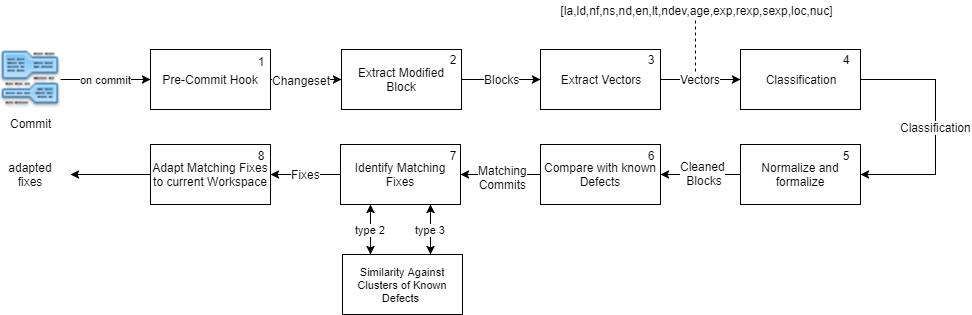
\includegraphics[width=\textwidth]{media/chap7/detect-approach}
    \caption{Classifying incoming commits and proposing fixes\label{fig:CLEVERT2}}
\end{figure*}

In the second process (Figure \ref{fig:CLEVERT2}), CLEVER intercepts
incoming commits before they leave a developer's workstation using the
concept of pre-commit hooks.

Ubisoft's developers already use pre-commit hooks for all sorts of
reasons such as identifying the tasks that are addressed by the commit
at hand, specifying the reviewers who will review the commit, and so on.
Implementing this part of CLEVER as a pre-commit hook is an important
step towards the integration of CLEVER with the workflow of developers
at Ubisoft. The developers do not have to download, install, and
understand additional tools in order to use CLEVER.

Once the commit is intercepted, we compute code and process metrics
associated with this commit. The selected metrics are discussed further
in Section \ref{sec:offline}. The result is a feature vector (Step 4)
that is used for classifying the commit as \emph{risky} or
\emph{non-risky}.

If the commit is classified as \emph{non-risky}, then the process stops,
and the commit can be transferred from the developer's workstation to
the central repository. \emph{Risky} commits, on the other hand, are
further analysed in order to reduce the number of false positives
(healthy commits that are detected as risky). We achieve this by first
extracting the code blocks that are modified by the developer and then
compare them to code blocks of known fault-introducing commits.

\subsection{Clustering Projects}\label{sec:clustering}

We cluster projects using the same technic as BIANCA (i.e.~Newman
algorithm {[}61, 143{]} on the dependcies) for the same reasons
(i.e.~projects that share dependencies are most likely to contain
defects caused by misuse of these dependencies).

Within the context of Ubisoft, dependencies can be \emph{external} or
\emph{internal} depending on whether the products are created in-house
or supplied by a third-party. For confidentiality reasons, we cannot
reveal the name of the projects involved in the project dependency
graph. We show the 12 projects in yellow color with their dependencies
in blue color in Figure \ref{fig:dep-graph}. In total, we discovered 405
distinct dependencies. Dependencies can be internal (i.e.~library
developed at Ubisoft) or external (i.e.~library provided by third
parties). The resulting partitioning is shown in Figure
\ref{fig:network-sample}.

\begin{figure*}
  \centering
    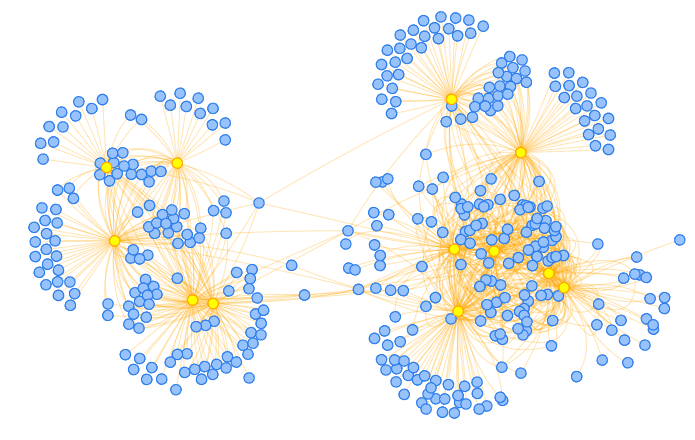
\includegraphics[width=\textwidth]{media/chap7/network.png}
    \caption{Dependency Graph\label{fig:dep-graph}}
\end{figure*}

At Ubisoft, dependencies are managed within the framework of a single
repository, which makes their automatic extraction possible. The
dependencies could also be automatically retrieved if the projects use a
dependency manager such as Maven.

\begin{figure*}
  \centering
    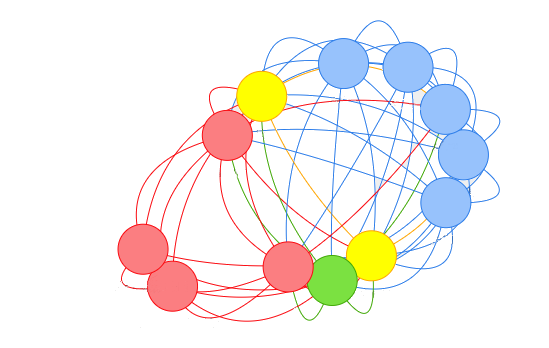
\includegraphics[width=0.7\textwidth]{media/chap7/network-sample.png}
    \caption{Clusters\label{fig:network-sample}}
\end{figure*}

\subsection{Building a Database of Code Blocks of Defect-Commits and
Fix-Commits}\label{sec:offline}

In order to build of database of code blocks of defect-commits and
fix-commits we use the same technic as for BIANCA. First, we listen to
issue closing-events and extract the blocks of code belonging to
incrimated commits (i.e.~commit known to have introduced a bug) using
our refined version of TXL and NICAD.

\subsection{Building a Metric-Based Model}\label{sec:metric-based}

We adapted Commit-guru {[}163{]} for building the metric-based model.
Commit-guru uses a list of keywords proposed by Hindle \emph{et al.}
{[}73{]} to classify commit in terms of \emph{maintenance},
\emph{feature} or \emph{fix}. Then, it uses the SZZ algorithm to find
the defect-commit linked to the fix-commit. For each defect-commit,
Commit-guru computes the following code metrics: \emph{la} (lines
added), \emph{ld} (lines deleted), \emph{nf} (number of modified files),
\emph{ns} (number of modified subsystems), \emph{nd} (number of modified
directories), \emph{en} (distriubtion of modified code across each
file), \emph{lt} (lines of code in each file (sum) before the commit),
\emph{ndev} (the number of developers that modifed the files in a
commit), \emph{age} (the average time interval between the last and
current change), \emph{exp} (number of changes previously made by the
author ), \emph{rexp} (experience weighted by age of files (1 / (n +
1))), \emph{sexp} (previous changes made by the author in the same
subsystem), \emph{loc} (total number of modified LOC across all files),
\emph{nuc} (number of unique changes to the files). Then, a statistical
model is built using the metric values of the defect-commits. Using
linear regression, Commit-guru is able to predict whether incoming
commits are \emph{risky} or not.

We had to modify Commit-guru to fit the context of this study. First, we
used information found in Ubisoft's internal project tracking system to
classify the purpose of a commit (i.e., \emph{maintenance},
\emph{feature} or \emph{fix}). In other words, CLEVER only classifies a
commit as a defect-commit if it is the root cause of a fix linked to a
crash or a bug in the internal project tracking system. Using internal
pre-commit hooks, Ubisoft developers must link every commit to a given
task \#ID. If the task \#ID entered by the developer matches a bug or
crash report within the project tracking system, then we perform the SCM
blame/annotate function on all the modified lines of code for their
corresponding files on the fix-commit's parents. This returns the
commits that previously modified these lines of code and are flagged as
defect-commits. Another modification consists of the actual
classification algorithm. We did not use linear regression but instead
the random forest algorithm {[}187, 188{]}. The random forest algorithm
turned out to be more effective as described in Section
\ref{sec:result-bianca}. Finally, we had to rewrite Commit-guru in
GoLang for performance and internal reasons.

\subsection{Comparing Code Blocks}\label{sec:online}

Each time a developer makes a commit, CLEVER intercepts it using a
pre-commit hook and classifies it as \emph{risky} or not. If the commit
is classified as \emph{risky} by the metric-based classifier, then, we
extract the corresponding code block (in a similar way as in the
previous phase), and compare it to the code blocks of historical
defect-commits. If there is a match, then the new commit is deemed to be
risky. A threshold \(\alpha\) is used to assess the extent beyond which
two commits are considered similar.

Once again, we reuse the comparing method approach created for BIANCA
when it comes to compare blocks of code.

\subsection{Classifying Incoming
Commits}\label{classifying-incoming-commits}

As discussed in Section \ref{sec:metric-based}, a new commit goes
through the metric-based model first (Steps 1 to 4). If the commit is
classified as \emph{non-risky}, we simply let it through, and we stop
the process. If the commit is classified as \emph{risky}, however, we
continue the process with Steps 5 to 8 in our approach.

One may wonder why we needed to have a metric-based model in the first
place. We could have resorted to clone detection as the main mechanism
as exposed in the previous chapter. The main reason for having the
metric-based model is efficiency. If each commit had to be analysed
against all known signatures using code clone similarity, then, it would
have made CLEVER impractical at Ubisoft's scale. We estimate that, in an
average workday (i.e.~thousands of commits), if all commits had to be
compared against all signatures on the same cluster we used for our
experiments it would take around 25 minutes to process a commit with the
current processing power dedicated to \emph{CLEVER}. In comparison, it
takes, on average, 3.75 seconds with the current two-step approach.

\subsection{Proposing Fixes}\label{proposing-fixes}

An important aspect in the design of CLEVER is the ability to provide
guidance to developers on how to improve risky commits. We achieve this
by extracting from the database the fix-commit corresponding to the top
1 matching defect-commits and present it to the developer. We believe
that this makes CLEVER a practical approach. Developers can understand
why a given modification has been reported as risky by looking at code
instead of simple metrics as in the case of the studies reported in
{[}91, 163{]}.

Finally, using the fixes of past defects, we can provide a solution, in
the form of a contextualised diff, to developers. A contextualised diff
is a diff that is modified to match the current workspace of the
developer regarding variable types and names. In Step 8 of Figure 3, we
adapt the matching fixes to the actual context of the developer by
modifying indentation depth and variable name in an effort to reduce
context switching. We believe that this would make it easier for
developers to understand the proposed fixes and see if it applies in
their situation.

All the proposed fixes will come from projects in the same cluster as
the project where the \emph{risky} commit is. Thus, developers have
access to fixes that should be easier to understand as they come from
projects similar to theirs inside the company.

\section{Experimental Setup}\label{sec:exp}

In this section, we present the setup of our case study in terms of
repository selection, dependency analysis, comparison process and
evaluation measures.

\subsection{Project Repository Selection}\label{sec:rep}

In collaboration with Ubisoft developers, we selected 12 major software
projects (i.e., systems) developed at Ubisoft to evaluate the
effectiveness of CLEVER. These systems continue to be actively
maintained by thousands of developers. Ubisoft projects are organized by
game engines. A game engine can be used in the development of many
high-budget games. The projects selected for this case study are related
to the same game engine. For confidentiality and security reasons,
neither the names nor the characteristics of these projects are
provided. We can, however, disclose that the size of these systems
altogether consists of millions of files of code, hundreds of millions
of lines of code and hundreds of thousands of commits. All 12 systems
are AAA videos games.

\subsection{Project Dependency Analysis}\label{sec:dependencies}

Figure \ref{fig:dep-graph} shows the project dependency graph. As shown
in Figure \ref{fig:dep-graph}, these projects are highly interconnected.
A review of each cluster shows that this partitioning divides projects
in terms of their high-level functionalities. For example, one cluster
is related to a given family of video games, whereas the other cluster
refers to another family. We showed this partitioning to 11 experienced
software developers and ask them to validate it. They all agreed that
the results of this automatic clustering are accurate and reflects well
the various project groups of the company. The clusters are used for
decreasing the rate of false positive. In addition, fixes mined across
projects but within the cluster are qualitative as shown in our
experiments.

\subsection{Building a Database of Defect-Commits and
Fix-Commits}\label{sub:golden}

To build the database that we can use to assess the performance of
CLEVER, we use the same process as discussed in Section
\ref{sec:offline}. We retrieve the full history of each project and
label commits as defect-commits if they appear to be linked to a closed
issue using the SZZ algorithm {[}100{]}. This baseline is used to
compute the precision and recall of CLEVER. Each time CLEVER classifies
a commit as \emph{risky}; we can check if the \emph{risky} commit is in
the database of defect-introducing commits. The same evaluation process
is used by related studies {[}24, 53, 91, 106, 116{]}.

\subsection{Process of Comparing New Commits}\label{sec:newcommits}

\begin{figure}
  \centering
    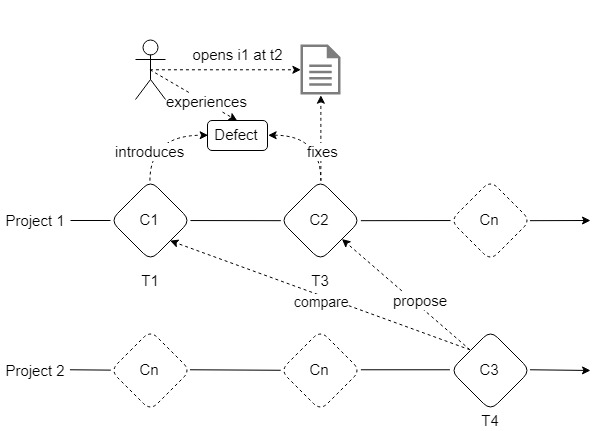
\includegraphics[width=0.5\textwidth]{media/chap7/comparing}
    \caption{Process of Comparing New Commits\label{fig:COMPARING}}
\end{figure}

Similarly to PRECINCT and CLEVER, the repository if cloned, rewinded and
replayed commit by commit in order to evaluate the performances of
CLEVER.

While figure \ref{fig:COMPARING} explains the processes of \emph{CLEVER}
it does not encompasse all the cases. Indeed, the user that experiences
the defect can be internal (i.e.~another developer, a tester, \ldots{})
or external (i.e.~a player). In addition, many other projects receive
commits in parallel and they are all to be compared with all the known
signatures.

\section{Empirical Validation}\label{sec:result-bianca}

In this section, we show the effectiveness of CLEVER in detecting risky
commits using a combination of metric-based models and clone detection.
The main research question addressed by this case study is: \emph{Can we
detect risky commits by combining metrics and code comparison within and
across related Ubisoft projects, and if so, what would be the accuracy?}

The experiments took nearly two months using a cluster of six 12 3.6 Ghz
cores with 32GB of RAM each. The most time consuming part of the
experiment consists of building the baseline as each commit must be
analysed with the SZZ algorithm. Once the baseline was established, the
model built, it took, on average, 3.75 seconds to analyse an incoming
commit on our cluster.

In the following subsections, we provide insights on the performance of
CLEVER by comparing it to Commit-guru {[}163{]} alone, i.e., an approach
that relies only on metric-based models. We chose Commit-guru because it
has been shown to outperform other techniques (e.g., {[}91, 106{]}).
Commit-guru is also open source and easy to use.

\subsection{Performance of CLEVER}\label{performance-of-clever}

When applied to 12 Ubisoft projects, CLEVER detects risky commits with
an average precision, recall, and F1-measure of 79.10\%, a 65.61\%, and
71.72\% respectively. For clone detection, we used a threshold of 30\%.
This is because Roy \emph{et al.} {[}166{]} showed through empirical
studies that using NICAD with a threshold of around 30\%, the default
setting, provides good results for the detection of Type 3 clones. When
applied to the same projects, Commit-guru achieves an average precision,
recall, and F1-measure of 66.71\%, 63.01\% and 64.80\%, respectively.

We can see that with the second phase of CLEVER (clone detection) there
is considerable reduction in the number of false positives (precision of
79.10\% for CLEVER compared to 66.71\% for Commit-guru) while achieving
similar recall (65.61\% for CLEVER compared to 63.01\% for Commit-guru).

\begin{table*}[]
\centering
\caption{Workshop results}
\label{tab:Workshop}
\resizebox{\textwidth}{!}{%
\begin{tabular}{c|c|c|c|c|c|c|c|c|c|c|c|c}
   & F1        & F2 & F3        & F4        & F5 & F6        & F7 & F8        & F9 & F10       & F11       & F12 \\ \hline
P1 & Accepted & Rejected   & Accepted & Accepted & Unsure  & Accepted & Unsure  & Rejected          & Rejected   & Accepted & Accepted & Unsure   \\
P2 & Accepted & Rejected   & Accepted & Unsure         & Unsure  & Accepted & Unsure  & Rejected          & Rejected   & Accepted & Accepted & Unsure   \\
P3 & Accepted & Rejected   & Accepted & Unsure         & Unsure  & Accepted & Unsure  & Rejected          & Rejected   & Accepted & Accepted & Unsure   \\
P4 & Accepted & Rejected   & Accepted & Unsure         & Unsure  & Accepted & Unsure  & Accepted & Rejected   & Accepted & Accepted & Unsure   \\
P5 & Accepted & Rejected   & Accepted & Accepted & Unsure  & Accepted & Unsure  & Rejected          & Rejected   & Accepted & Accepted & Unsure   \\
P6 & Accepted & Rejected   & Accepted & Unsure         & Unsure  & Accepted & Unsure  & Accepted & Rejected   & Accepted & Accepted & Unsure   \\ \hline
\end{tabular}
}
\end{table*}

\subsection{Analysis of the Quality of the Fixes Proposed by
CLEVER}\label{analysis-of-the-quality-of-the-fixes-proposed-by-clever}

In order to validate the quality of the fixes proposed by CLEVER, we
conducted an internal workshop where we invited a number of people from
Ubisoft development team. The workshop was attended by six participants:
two software architects, two developers, one technical lead, and one IT
project manager. The participants have many years of experience at
Ubisoft.

The participants were asked to review 12 randomly selected fixes that
were proposed by CLEVER. These fixes are related to one system in which
the participants have excellent knowledge. We presented them with the
original buggy commits, the original fixes for these commits, and the
fixes that were automatically extracted by CLEVER. We asked them the
following question \emph{``Is the proposed fix applicable in the given
situation?''} for each fix.

The review session took around 50 minutes. This does not include the
time it took to explain the objective of the session, the setup, the
collection of their feedback, etc.

We asked the participants to rank each fix proposed by CLEVER using this
scheme:

\begin{itemize}
\tightlist
\item
  Fix Accepted: The participant found the fix proposed by CLEVER
  applicable to the risky commit.
\item
  Unsure: In this situation, the participant is unsure about the
  relevance of the fix. There might be a need for more information to
  arrive to a verdict.
\item
  Fix Rejected: The participant found the fix is not applicable to the
  risky commit.
\end{itemize}

Table \ref{tab:Workshop} shows answers of the participants. The columns
refer to the fixes proposed by CLEVER, whereas the rows refer to the
participants that we denote using P1, P2, \ldots{}, P6. As we can see
from the table, 41.6\% of the proposed fixes (F1, F3, F6, F10 and F12)
have been accepted by all participants, while 25\% have been accepted by
at least one member (F4, F8, F11). We analysed the fixes that were
rejected by some or all participants to understand the reasons.

\(F2\) was rejected by our participants because the region of the commit
that triggered a match is a generated code. Although this generated code
was pushed into the repositories as part of bug fixing commit, the root
cause of the bug lies in the code generator itself. Our proposed fix
suggests to update the generated code. Because the proposed fix did not
apply directly to the bug and the question we ask our reviewers was
\emph{``Is the proposed fix applicable in the given situation?''} they
rejected it. In this occurrence, the proposed fix was not applicable.

\(F4\) was accepted by two reviewers and marked as unsure by the other
participants. We believe that this was due the lack of context
surrounding the proposed fix. The participants were unable to determine
if the fix was applicable or not without knowing what the original
intent of the buggy commit was. In our review session, we only provided
the reviewers with the regions of the commits that matched existing
commits and not the full commit. Full commits can be quite lengthy as
they can contain asset descriptions and generated code, in addition to
the actual code. In this occurrence, the full context of the commit
might have helped our reviewers to decide if \(F4\) was applicable or
not. \(F5\) and \(F7\) were classified as unsure by all our participants
for the same reasons.

\(F8\) was rejected by four of participants and accepted by two. The
participants argued that the proposed fix was more a refactoring
opportunity than an actual fix.

\(F12\) was marked as unsure by all the reviewers because the code had
to do with a subsystem that is maintained by another team and the
participants felt that it was out of the scope of this session.

After the session, we asked the participants two additional questions:
\emph{Will you use CLEVER in the future?} and \emph{What aspects of
CLEVER need to be improved?}

All the participants answered the first question favourably. They also
proposed to embed CLEVER with Ubisoft's quality assurance tool suite.
The participants reported that the most useful aspects of CLEVER are:

\begin{itemize}
\tightlist
\item
  Ability to leverage many years of historical data of inter-related
  projects, hence allowing development teams to share their experiences
  in fixing bugs.
\item
  Easy integration of CLEVER into developers' work flow based on the
  tool's ability to operate at commit-time.\\
\item
  Precision and recall of the tool (79\% and 65\% respectively)
  demonstrating CLEVER's capabilities to catch many defects that would
  otherwise end up in the code repository. For the second question, the
  participants proposed to add a feedback loop to CLEVER where the input
  of software developers is taken into account during classification.
  The objective is to reduce the number of false negatives (risky
  commits that are flagged as non-risky) and false positives (non-risky
  commits that are flagged as risky). The feedback loop mechanism would
  work as follows: When a commit is misclassified by the tool, the
  software developer can choose to ignore CLEVER's recommendation and
  report the misclassified commit. If the fix proposition is not used,
  then, we would give that particular pattern less strength over other
  patterns automatically.
\end{itemize}

We do not need manual input from the user because CLEVER knows the state
of the commit before the recommendation and after. If both versions are
identical then we can mark the recommendation as not helpful. This way,
we can also compensate for human error (i.e., a developer rejecting
CLEVER recommendation when the commit was indeed introducing a defect.
We would know this by using the same processes that allowed us to build
our database of defect-commits as described in Section
\ref{sec:offline}. This feature is currently under development.

It is worth noting that Ubisoft developers who participated to this
study did not think that CLEVER fixes that were deemed irrelevant were a
barrier to the deployment of CLEVER. In their point of view, the
performance of CLEVER in terms of classification should make a
significant impact as suspicious commits will receive extended reviews
and/or further investigations.

We are also investigating the use of adaptive learning techniques to
improve the classification mechanism of CLEVER. In addition to this, the
participants discussed the limitation of CLEVER as to its inability to
deal with automatically generated code. We are currently working with
Ubisoft's developers to address this limitation.

\section{University-Industry Research
Collaboration}\label{university-industry-research-collaboration}

In this section, we describe the lessons learned during this industrial
collaboration.

\subsection{Deep understanding of the project
requirements}\label{deep-understanding-of-the-project-requirements}

Throughout the design of CLEVER, it was important to have a close
collaboration between the research team and the Ubisoft developers. This
allowed the research team to understand well the requirements of the
project. Through this collaboration, both the research and development
teams quickly realized that existing work in the literature was not
sufficient to address the project's requirements. In addition, existing
studies were mainly tested using open source systems, which may be quite
different in structure and size from large industrial systems. In our
case, we found that a deep understanding of Ubisoft ecosystem was an
important enabler for many decisions we made in this project including
the fact that CLEVER operates on multiple systems and that it uses a
two-phase mechanism. It was also important to come up with a solution
that integrates well with the workflow of Ubisoft developers. This
required the development of CLEVER in a way it integrates well with the
entire suite of Ubisoft's version control systems. The key lesson here
is to understand well the requirements of a project and its complexity.

\subsection{Understanding the benefits of the project to both
parties}\label{understanding-the-benefits-of-the-project-to-both-parties}

Understanding how the project benefits the company and the university
helps both parties align their vision and work towards a common goal and
set of objectives. From Ubisoft's perspective, the project provides
sound mechanisms for building reliable systems. In addition, the time
saved from detecting and fixing defects can be shifted to the
development of new functionalities that add value to Ubisoft customers.
For the university research team, the project provides an excellent
opportunity for gaining a better understanding of the complexity of
industrial systems and how research can provide effective and practical
solutions. Also, working closely with software developers helps uncover
the practical challenges they face within the company's context.
Companies vary significantly in terms of culture, development processes,
maturity levels, etc. Research effort should be directed to develop
solutions that overcome these challenges, while taking into account the
organizational context.

\subsection{Focusing in the Beginning on Low-Hanging
Fruits}\label{focusing-in-the-beginning-on-low-hanging-fruits}

Low-hanging fruits are quick fixes and solutions. We found that it is a
good idea to showcase some quick wins early in the project to show the
potential of the proposed solutions. At the beginning of the project, we
applied the two-phase process of CLEVER to some small systems with a
reasonable number of commits. We showed that the approach improved over
the use of metrics alone. We also showed that CLEVER was able to make
suggestions on how to fix the detected risky commits. This encouraged us
to continue on this path and explore additional features. We continued
to follow an iterative and incremental process throughout the project
where knowledge transition between the University and Ubisoft teams is
done on a regular basis. Building a Strong Technical Team: Working on
industrial projects requires all sort of technical skills including
programming in various programming languages, the use of tools, tool
integration, etc. The strong technical skills of the lead student of
this project were instrumental in the success of this project. It should
be noted that Ubisoft systems are programmed using different languages,
which complicated the code matching phase of CLEVER. In addition,
Ubisoft uses multiple bug management and version control systems.
Downloading, processing, and manipulating commits from various
environment requires excellent technical abilities.

\subsection{Communicating effectively}\label{communicating-effectively}

During the development of CLEVER, we needed to constantly communicate
the steps of our research to developers and project owners. Adopting a
communication strategy suitable to each stakeholder was important. For
example, in our meetings with management, we focused more on the ability
of CLEVER to improve code quality and reduce maintenance costs instead
of the technical details of the proposed approach. Developers, on the
other hand, were interested in the potential of CLEVER and its
integration with their work environment.

In this talk, we share our experience conducting a research project at
Ubisoft. The project consists of developing techniques and a tool for
detecting defects before they reach the code repository. Our approach,
called CLEVER, achieves this in two phases using a combination of
metric-based machine learning models and clone detection. CLEVER is
being deployed at Ubisoft.

\subsection{Managing change}\label{managing-change}

Any new initiate brings with it important changes to the way people
work. Managing these changes from the beginning of the project increases
the chances for tool adoption. To achieve this, we used a communication
strategy that involved all the stakeholders including software
developers and management to make sure that potential changes that
CLEVER would bring are thoroughly and smoothly implemented, and that the
benefits of change are long-lasting.

\section{Threats to Validity}\label{threats-to-validity-3}

We identified two main limitations of our approach, CLEVER, which
require further studies.

CLEVER is designed to work on multiple related systems. Applying CLEVER
to a single system will most likely be less effective. The two-phase
classification process of CLEVER would be hindered by the fact that it
is unlikely to have a large number of similar bugs within the same
system. For single systems, we recommend the use of metric-based models.
A metric-based solution, however, may turn to be ineffective when
applied across systems because of the difficulty associated with
identifying common thresholds that are applicable to a wide range of
systems.

The second limitation we identified has to do with the fact that CLEVER
is designed to work with Ubisoft systems. Ubisoft uses C\#, C, C++, Java
and other internally developed languages. It is however common to have
other languages used in an environment with many inter-related systems.
We intend to extend CLEVER to process commits from other languages as
well.

The selection of target systems is one of the common threats to validity
for approaches aiming to improve the analysis of software systems. It is
possible that the selected programs share common properties that we are
not aware of and therefore, invalidate our results. Because of the
industrial nature of this study, we had to work with the systems
developed by the company.

The programs we used in this study are all based on the C\#, C, C++ and
Java programming languages. This can limit the generalization of the
results to projects written in other languages, especially that the main
component of CLEVER is based on code clone matching.

Finally, part of the analysis of the CLEVER proposed fixes that we did
was based on manual comparisons of the CLEVER fixes with those proposed
by developers with a focus group composed of experienced engineers and
software architects. Although, we exercised great care in analysing all
the fixes, we may have misunderstood some aspects of the commits.

In conclusion, internal and external validity have both been minimized
by choosing a set of 12 different systems, using input data that can be
found in any programming languages and version systems (commits and
changesets).

\section{Chapter Summary}\label{chapter-summary-3}

In this chapter, we presented CLEVER (Combining Levels of Bug Prevention
and Resolution Techniques), an approach that detects risky commits
(i.e., a commit that is likely to introduce a bug) with an average of
79.10\% precision and a 65.61\% recall. CLEVER combines code metrics,
clone detection techniques, and project dependency analysis to detect
risky commits within and across projects. CLEVER operates at
commit-time, i.e., before the commits reach the central code repository.
Also, because it relies on code comparison, CLEVER does not only detect
risky commits but also makes recommendations to developers on how to fix
them. We believe that this makes CLEVER a practical approach for
preventing bugs and proposing corrective measures that integrate well
with the developer's workflow through the commit mechanism. CLEVER is
still in its infancy and we expect it to be available this year to
thousands of developers.

In the next chapter, we present JCHARMING, an approach for reproducing bugs
using stack traces. JCHARMING is meant to be used
by developers when the commit-time approaches presented in Chapters 4, 6
and 7 did not manage to prevent the introduction of defects.

\chapter{Bug Reproduction Using Crash Traces and Directed Model
Checking}\label{bug-reproduction-using-crash-traces-and-directed-model-checking}

In previous chapters, we presented three approaches (PRECINCT, BIANCA
and, CLEVER) that aim to improve code quality by performing
maintenance operations at commit-time. While these approaches have shown
to be effective, they can never be 100\% accurate. Therefore, we need to contribute with methods that can help fix crashes after they occur.

The first (and perhaps main) step in understanding the cause of a field
crash is to reproduce the bug that caused the system to fail. A survey
conducted with developers of major open source software systems such as
Apache, Mozilla and Eclipse revealed that one of the most valuable piece
of information that can help locate and fix the cause of a crash is the
one that can help reproduce it {[}22{]}.

Bug reproduction is, however, a challenging task because of the limited
amount of information provided by the end users. There exist several bug
reproduction techniques. They can be grouped into two categories: (a)
On-field record and in-house replay {[}9, 80, 133{]}, and (b) In-house
crash explanation {[}{[}122{]}; chandra2009snugglebug{]}. The first
category relies on instrumenting the system in order to capture objects
and other system components at run-time. When a faulty behavior occurs
in the field, the stored objects, as well as the entire heap, are sent
to the developers along with the faulty methods to reproduce the crash.
These techniques tend to be simple to implement and yield good results,
but they suffer from two main limitations. First, code instrumentation
comes with a non-negligible overhead on the system. The second
limitation is that the collected objects may contain sensitive
information causing customer privacy issues. The second category is
composed of tools leveraging proprietary data in order to provide hints
on potential causes. While these techniques are efficient in improving
our comprehension of the bugs, they are not designed with the purpose of
reproducing them.

JCHARMING (Java CrasH Automatic Reproduction by directed Model checkING)
{[}137{]} is a hybrid approach that uses a combination of crash traces
and model checking to reproduce bugs that caused field failures
automatically. Unlike existing techniques, JCHARMING does not require
instrumentation of the code. It does not need access to the content of
the heap either. Instead, JCHARMING uses the list of functions, i.e.,
the crash trace, that are output when an uncaught exception in Java
occurs to guide a model checking engine to uncover the statements that
caused the crash. Note that a crash trace is sometimes referred to as a
stack trace. In this paper, we use these two terms interchangeably.

Model checking (also known as property checking) is a formal technique
for automatically verifying a set of properties of finite-state systems
{[}13{]}. More specifically, this technique builds a graph where each
node represents one state of the program and the set of properties that
need to be verified in each state. For real-world programs, model
checking is often computationally impracticable because of the state
explosion problem {[}13{]}. To address this challenge and apply model
checking on large programs, we direct the model checking engine towards
the crash using program slicing and the content of the crash trace, and
hence, reduce the search space. When applied to reproducing bugs of
seven open source systems, JCHARMING achieved 85\% accuracy.

The accuracy of JCHARMING, when applied to 30 bugs, is 80\%.

\section{\texorpdfstring{Preliminaries\label{sec:prelimenaries}}{Preliminaries}}\label{preliminaries}

Model checking (also known as property checking) will, given a formally
defined system (that could be software {[}193{]} or hardware based
{[}109{]}), check if the system meets a specification by testing
exhaustively all the states of the system under test (SUT), which can be
represented by a Kripke {[}108{]} structure:

\begin{equation}
SUT = <S, S_0, T, L>
\end{equation}

where \(S\) is a set of states, \(S_0\) the set of initial states, \(T\)
the transitions relations between states and \(L\) the labeling
function, which labels a state with a set of atomic properties. Figure
\ref{fig:mc-def} presents a system with four steps \(S_0\) to \(S_3\),
which have five atomic properties \(p_1\) to \(p_5\). The labeling
function \(L\) gives us the properties that are true in a state:
\(L(S_0) = {p_1}, L(S_1) = {p_1, p_2}, L(S_2) = {p_3}, L(S_3) = {p_4, p_5}\).

\begin{figure}[h!]
  \centering
    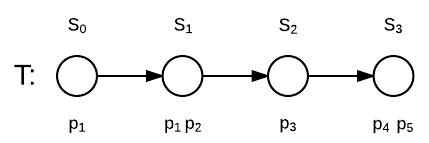
\includegraphics[scale=0.4]{media/chap8/mc-def.png}
    \caption{System with four steps $S_0$ to $S_3$, which have five atomic properties $p_1$ to $p_5$
    \label{fig:mc-def}}
\end{figure}

The SUT is said to satisfy a property \(p\) at a given time if there
exists a sequence of states \(x\) leading to a state where \(p\) holds.
This can be written as:

\begin{equation}
(SUT, x) \models p
\end{equation}

For the SUT of Figure \ref{fig:mc-def}, we can write
\((SUT, {S_0, S_1, S_2})\) \(\models\) \(p_3\) because the sequence of
states \({S_0, S_1, S_2}\) will lead to a state \(S_2\) where \(p_3\)
holds. However,

\begin{equation}
(SUT, S_0, S_1, S_2) \models p_3
\end{equation}

only ensures that \(\exists x\) such that \(p\) is reached at some point
in the execution of the program and not that \(p_3\) holds for
\(\forall x\).

In JCHARMING, we assume that SUTs must not crash in a typical
environment. In the framework of this study, we consider a typical
environment as any environment where the transitions between the states
represent the functionalities offered by the program. For example, in a
typical environment, the program heap or other memory spaces cannot be
modified. Without this constraint, all programs could be tagged as buggy
since we could, for example, destroy objects in memory while the program
continues its execution. As we are interested in verifying the absence
of unhandled exceptions in the SUT, we aim to verify that for all
possible combinations of states and transitions there is no path leading
towards a crash. That is:

\begin{equation}
\forall x.(SUT, x) \models \neg c
\end{equation}

If there exists a contradicting path (i.e., \(\exists x\) such that
\((SUT, x) \models c\)) then the model checker engine will output the
path \(x\) (known as the counter-example), which can then be executed.
The resulting Java exception crash trace is compared with the original
crash trace to assess if the bug is reproduced. While being accurate and
exhaustive in finding counter-examples, model checking suffers from the
state explosion problem, which hinders its applicability to large
software systems.

To show the contrast between testing and model checking, we use the
hypothetical example of Figures \ref{fig:testing-toy},
\ref{fig:checking-toy} and \ref{fig:dchecking-toy} and sketch the
possible results of each approach. These figures depict a toy program
where from the entry point, unknown calls are made (dotted points) and,
at some points, two methods are called. These methods, called
\texttt{Foo.Bar} and \texttt{Bar.Foo}, implement a \texttt{for loop}
from 0 to \texttt{loopCount}. The only difference between these two
methods is that the \texttt{Bar.Foo} method throws an exception if \(i\)
becomes larger than two. Hereafter, we denote this property as
\(p_{i > 2}\).

\begin{figure}
  \centering
    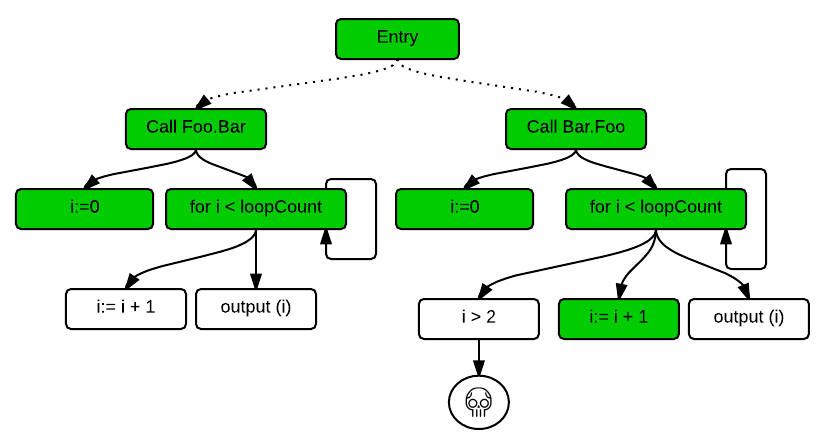
\includegraphics[scale=0.8]{media/chap8/test.png}
    \caption{A toy program under testing
    \label{fig:testing-toy}}
\end{figure}

\begin{figure}
  \centering
    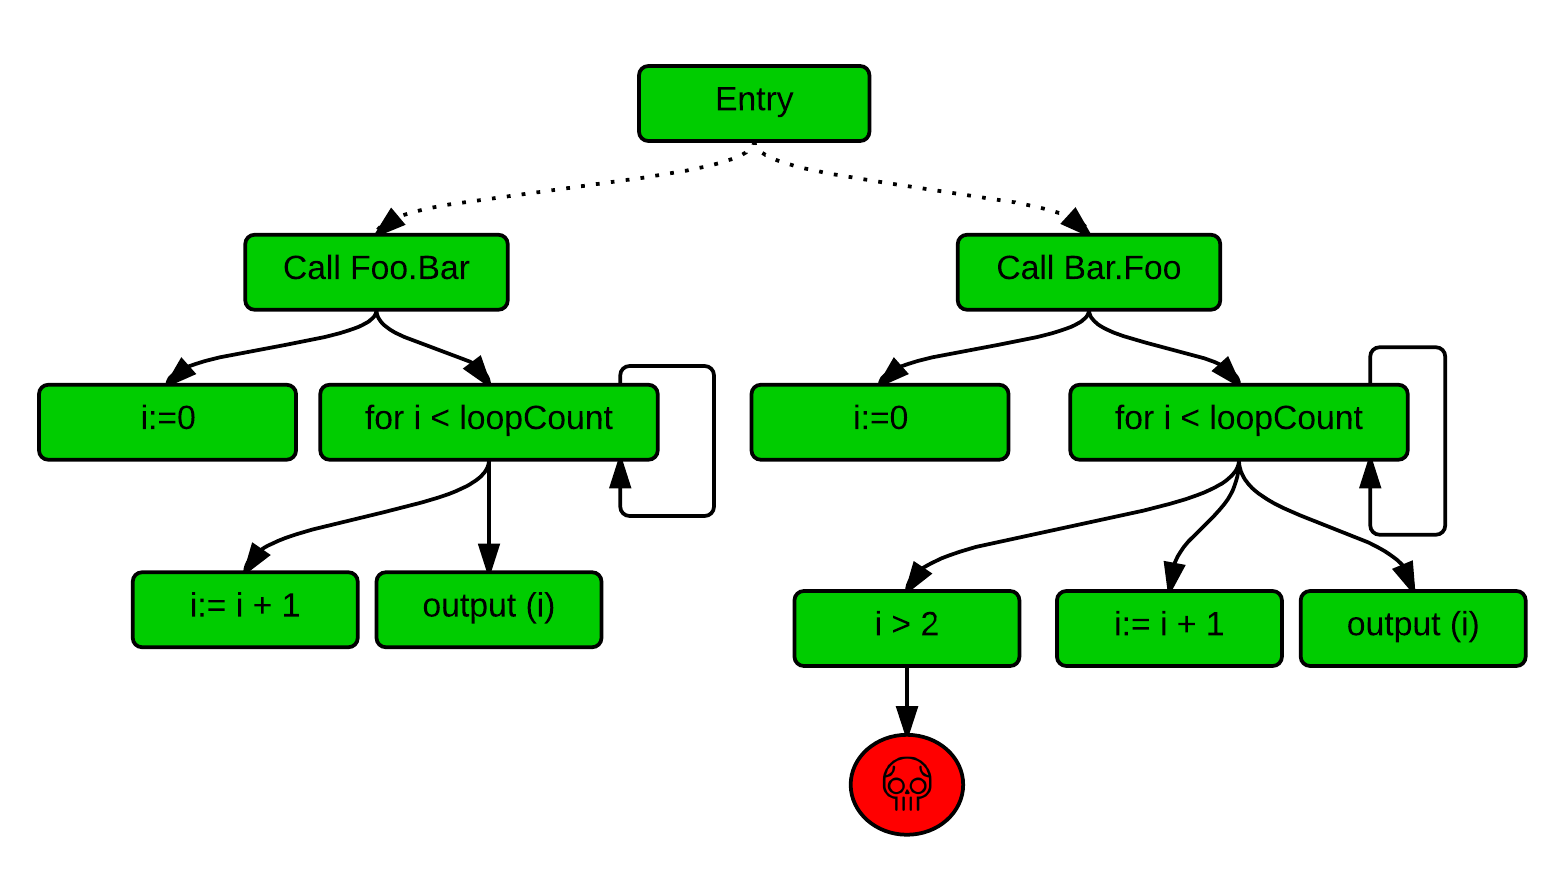
\includegraphics[scale=0.8]{media/chap8/mc.png}
    \caption{A toy program under model checking
    \label{fig:checking-toy}}
\end{figure}

\begin{figure}
  \centering
    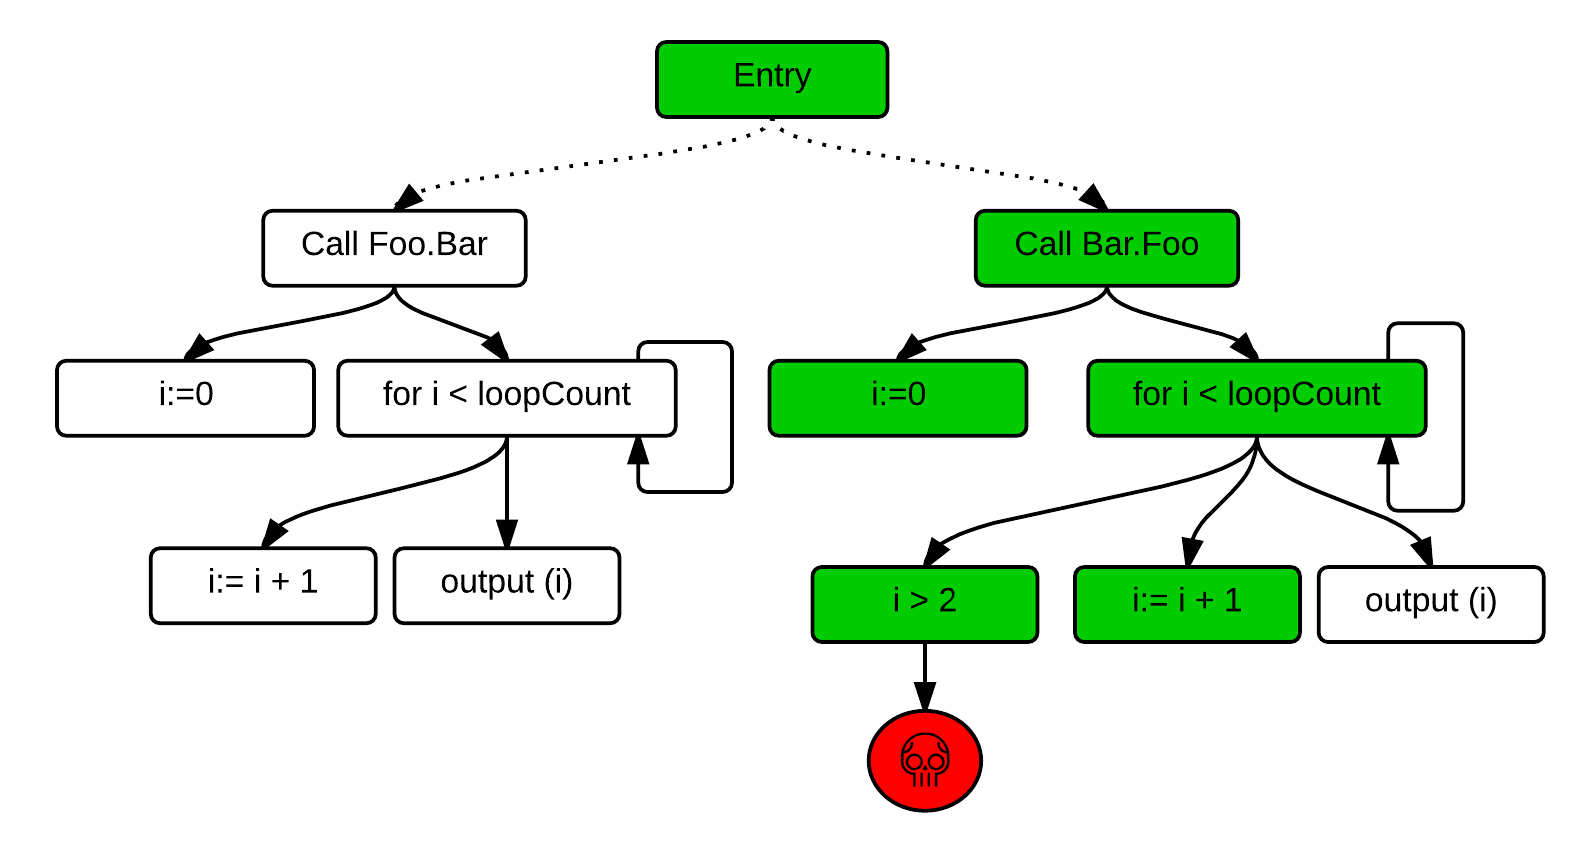
\includegraphics[scale=0.8]{media/chap8/dmc.png}
    \caption{A toy program under directed model checking
    \label{fig:dchecking-toy}}
\end{figure}

Figure \ref{fig:testing-toy} shows the program statements that could be
covered using testing approaches. Testing software is a demanding task
where a set of techniques is used to test the SUT according to some
input. Software testing depends on how well the tester understands the
SUT in order to write relevant test cases that are likely to find errors
in the program. Program testing is usually insufficient because it is
not exhaustive. In our case, using testing will mean that the tester
knows what to look for in order to detect the causes of the failure. We
do not assume this knowledge in JCHARMING.

Model checking, on the other hand, explores each and every state of the
program (Figure \ref{fig:checking-toy}), which makes it complete, but
impractical for real-world and large systems. To overcome the state
explosion problem of model checking, directed (or guided) model checking
has been introduced {[}51, 52{]}. Directed model checking uses insights
--- generally heuristics --- about the SUT in order to reduce the number
of states that need to be examined. Figure \ref{fig:dchecking-toy}
explores only the states that may lead to a specific location, in our
case, the location of the fault. The challenge, however, is to design
techniques that can guide the model checking engine. As we will describe
in the next section, we use crash traces and program slicing to overcome
this challenge.

Unlike model checking, directed model checking is not complete. In this
work, our objective is not to ensure absolute correctness of the
program, but to use directed model checking to ``hunt'' for a bug within
the program.

\section{\texorpdfstring{Approach\label{sec:jcharming}}{Approach}}\label{approach-4}

Figure \ref{fig:jcarming-approach} shows an overview of JCHARMING. The
first step consists of collecting crash traces, which contain raw lines
displayed to the standard output when an uncaught exception in Java
occurs. In the second step, the crash traces are preprocessed by
removing noise (mainly calls to Java standard library methods). The next
step is to apply backward slicing using static analysis to expand the
information contained in the crash trace while reducing the search
space. The resulting slice along with the crash trace are given as input
to the model checking engine. The model checker executes statements
along the paths from the main function to the first line of the crash
trace (i.e., the last method executed at crash time, also called the
crash location point). Once the model checker finds inconsistencies in
the program leading to a crash, we take the crash stack generated by the
model checker and compare it to the original crash trace (after
preprocessing). The last step is to build a JUnit test, to be used by
software engineers to reproduce the bug in a deterministic way.

\begin{figure}
  \centering
    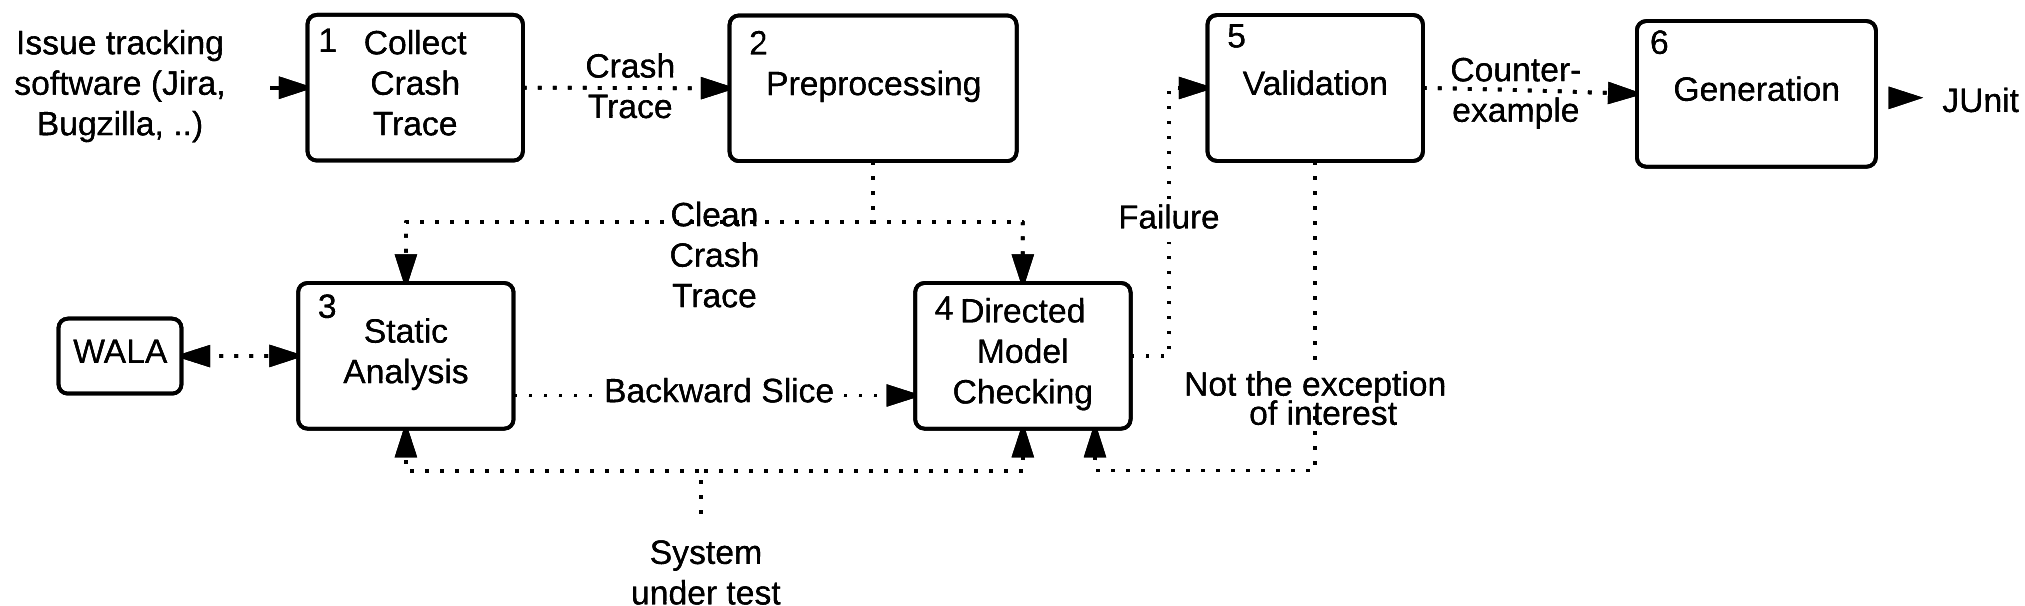
\includegraphics[scale=0.9]{media/chap8/jcharming-approach.png}
    \caption{Overview of JCHARMING.
    \label{fig:jcarming-approach}}
\end{figure}

\subsection{Collecting Crash Traces}\label{collecting-crash-traces}

The first step of JCHARMING is to collect the crash trace caused by an
uncaught exception. Crash traces are usually included in crash reports
and can, therefore, be automatically retrieved using a simple regular
expression. Figure \ref{fig:jcarming-traces} shows an example of a crash
trace that contains the exception thrown when executing the program
depicted in Figures \ref{fig:testing-toy} to \ref{fig:dchecking-toy}.
More formally, we define a Java crash trace \(T\) of size \(N\) as an
ordered sequence of frames \(T={f_0, f_1, f_2, ..., f_N}\). A frame
represents either a method call (with the location of the called method
in the source code), an exception, or a wrapped exception. In Figure
\ref{fig:jcarming-traces}, the frame \(f_0\) represents an exception,
the frame \(f_7\) represents a method call to the method
\texttt{jsep.Foo.buggy}, declared in file \texttt{Foo.java} at line 17.
In this example, this is the method that caused the exception. \(F_6\)
represents a wrapped exception.

It is common in Java to have crash traces that contain wrapped
exceptions. Such crash traces are incomplete in the sense that they do
not show all the method calls that are invoked from the entry point of
the program to the crash point. According to the Java documentation
{[}150{]}, line 8 of Figure \ref{fig:jcarming-traces} should be
interpreted as follows: \_``This line indicates that the remainder of
the stack trace for this exception matches the indicated number of
frames from the bottom of the stack trace of the exception that was
caused by this exception (the''enclosing exception``). This shorthand
can greatly reduce the length of the output in the common case where a
wrapped exception is thrown from the same method as the''causative
exception" is caught.``\_

We are likely to find shortened traces in bug repositories as they are
what the user sees without any possibility to expand their content.

\begin{figure}
  \noindent\fbox{%
      \parbox{\textwidth}{%
  1.javax.activity.InvalidActivityException:loopTimes \\
  should be $<$ 3 \\
  2. at Foo.bar(Foo.java:10) \\
  3. at GUI.buttonActionPerformed(GUI.java:88) \\
  4. at GUI.access\$0(GUI.java:85) \\
  5. at GUI\$1.actionPerformed(GUI.java:57) \\
  6. caused by java.lang.IndexOutOfBoundsException : 3 \\
  7. at jsep.Foo.buggy(Foo.java:17) \\
  8. and 4 more ...
      }%
  }
    \caption{Java InvalidActivityException is thrown in the Bar.Foo loop if the control variable is greater than~2.
    \label{fig:jcarming-traces}}
\end{figure}

In more details, Figure \ref{fig:jcarming-traces} contains a call to the
\(Bar.foo()\) method -- the crash location point -- and calls to Java
standard library functions (in this case, GUI methods because the
program was launched using a GUI). As shown in Figure
\ref{fig:jcarming-traces}, we can see that the first line (referred to
as frame \emph{\(f_0\)}, subsequently the next line is called frame
\emph{\(f_1\)}, etc.) does not represent the real crash point but it is
only the last exception of a chain of exceptions. Indeed, the
\(InvalidActivity\) has been triggered by an
\(IndexOutOfBoundsException\) in \(jsep.Foo.buggy\). This crash trace
shows also an example of nested try-catch blocks.

\subsection{Preprocessing}\label{preprocessing}

In the preprocessing step, we first reconstruct and reorganize the crash
trace in order to address the problem of nested exceptions. Nested
exception refers to the following structure in Java.

\noindent\fbox{%
  \parbox{\textwidth}{%

1 java.io.IOException: Spill failed \\
... \\
14 Caused by: java.lang.IllegalArgumentException \\
... \\
28 Caused by: java.lang.NullPointerException \\
    }%
 }

In such a case, we want to reproduce the root exception (line 28) that
led to the other two (lines 14 and 1). This said, we remove the lines 1
to 14. Then, with the aim to guide the directed model checking engine
optimally, we remove frames that are beyond our control. These refer to
Java library methods and third party libraries. In Figure
\ref{fig:jcarming-traces}, we can see that Java GUI and event management
components appear in the crash trace. We assume that these methods are
not the cause of the crash; otherwise, it means that there is something
wrong with the JDK itself. If this is the case, we will not be able to
reproduce the crash. Note that removing these unneeded frames will also
reduce the search space of the model checker.

\subsection{Building the Backward Static
Slice}\label{building-the-backward-static-slice}

Static analysis of programs consists of analyzing programs without
executing them or making assumptions about the inputs of the program.
There exist many techniques to perform static analysis (data flow
analysis, control flow analysis, theorem proving, etc.) that can be used
for debugging, program comprehension, and performance analysis. Static
slice is a type of static analysis, which takes a program and slicing
properties as input in order to create a smaller program with respect to
the slicing properties. An example of slicing properties could be to
extract only the program statements that modify a certain variable.
Static slicing is particularly interesting for JCHARMING as the sliced
program, being smaller, will have a smaller state space. We illustrate
the process of static slicing using the example in Figure
\ref{fig:slicing}. In this figure, we show an example of an abstract
syntax tree, generated from a given a program (not shown in this paper).
The black states could be states that are impacted by given slicing
properties. After the slicing, the final static slice contains the black
states and the states that are needed to reach them.

\begin{figure}
  \centering
    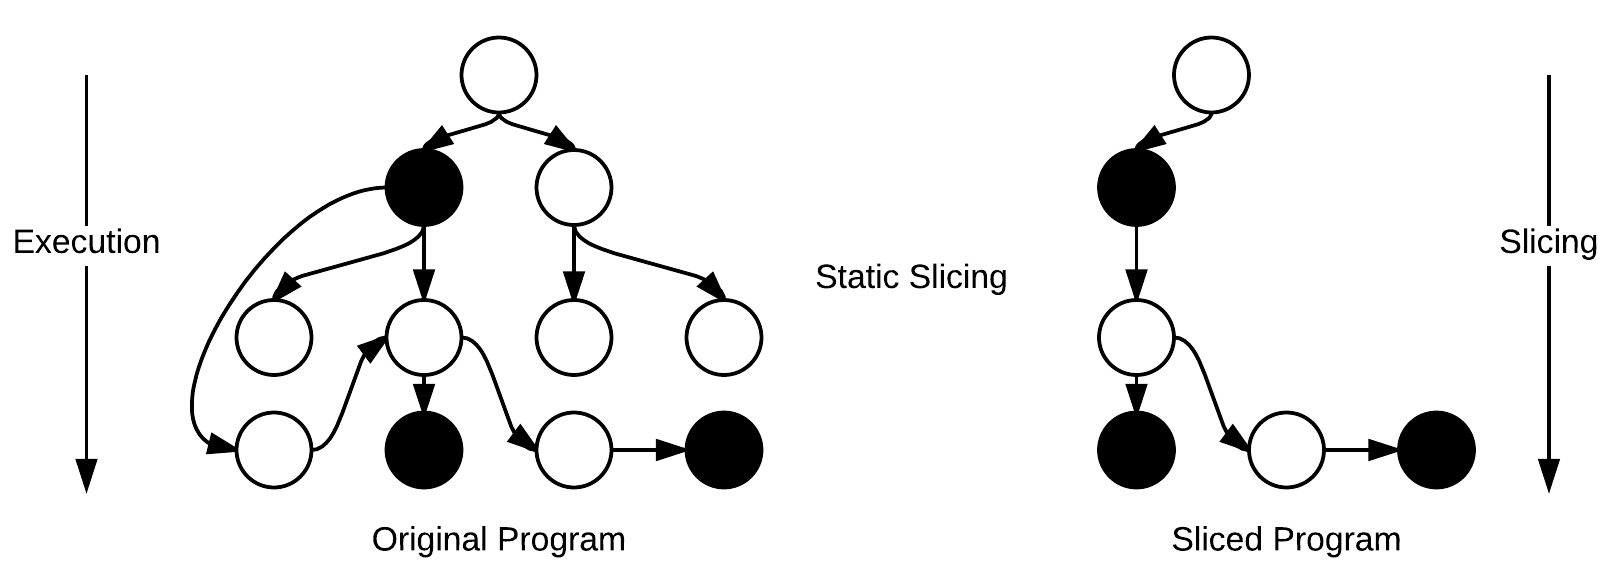
\includegraphics[scale=.2]{media/chap8/slicing.png}
    \caption{Hypothetical example of static program slicing\label{fig:slicing}}
\end{figure}

In JCHARMING, we use a particular static slicing known as backward
static slicing {[}44{]}. A backward slice contains all possible branches
that may lead to a point \emph{n} in the program from a point \emph{m}
as well as the definition of the variables that control these branches
{[}44{]}. In other words, the slice of a program point \emph{n} is the
program subset that may influence the reachability of point \emph{n}
starting from point \emph{m}. The backward slice containing the branches
and the definition of the variables leading to \emph{n} from \emph{m} is
noted as \(bslice_{[m \leftarrow n]}\). Figure
\ref{fig:backward-slicing} presents an example of a backward static
slice.

\begin{figure}
  \centering
    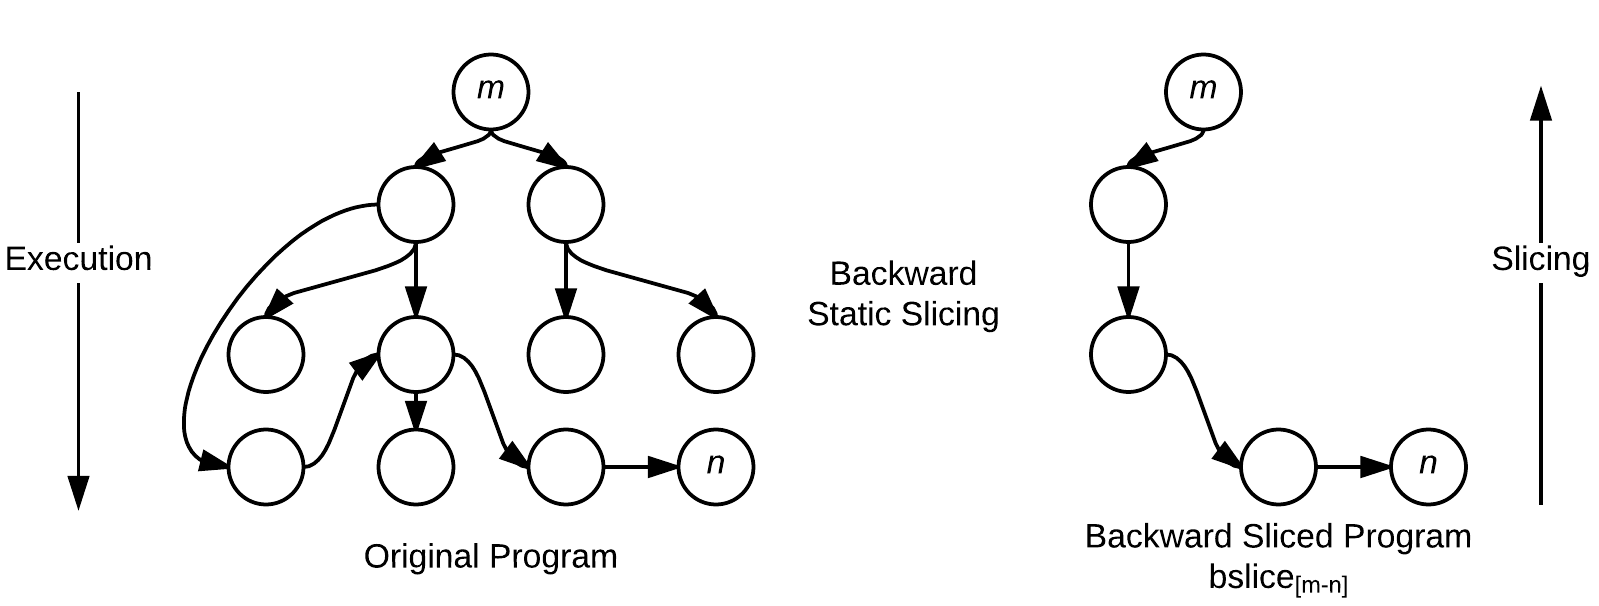
\includegraphics[scale=.2]{media/chap8/backward-slicing.png}
    \caption{Hypothetical example of backward static program slicing\label{fig:backward-slicing}}
\end{figure}

In JCHARMING, we compute a backward static slice between the location of
the crash (which we have in the crash trace) and the entry point of the
program (i.e., the main function). However, for large systems, a crash
trace does not necessarily contain all the methods that have been
executed starting from the entry point of the program to the crash
location point. We need to complete the content of the crash trace by
identifying all the statements that have been executed starting from the
main function until the last line of the preprocessed crash trace. In
Figure \ref{fig:jcarming-traces}, this will be the function call
\lstinline!Bar.Foo()! which happens to be also the crash location point.
To achieve this, we turn to static analyses by extracting a backward
slice from the main function of the program to the \lstinline!Bar.Foo()!
method.

\begin{equation}
bslice_{[f_n \leftarrow f_0]} = bslice_{[f_1 \leftarrow f_0]} \cup bslice_{[f_2 \leftarrow f_1]} \cup ... \cup bslice_{[f_n \leftarrow f_{n\mymathhyphen1}]}
\end{equation}

Note that the union of the slices computed between each pair of frames
must be a subset of the final slice between \(f_0\) and the entry point
of the program \(f_n\). More formally:

\begin{equation}
\bigcup_{i=0}^{n-1} bslice_{[f_{i+1} \leftarrow f_i]} \subseteq bslice_{[f_n \leftarrow f_0]}
\label{eq:slice-unions}
\end{equation}

Figure \ref{fig:jcharming-slice} presents an example that will help
understand Equation \ref{eq:slice-unions}. In this example, a toy
program composed of six methods \(a...f\) crashes in \(d\) with a crash
trace \(T = \{e, f, d\}\). The backward static slice from the crash
point \(d\) to the entry point \(a\) without using \(T\) will be
\(\{a, b, c, d, e, f\}\) as we do not assume to know the path taken to
reach \(d\). However, if we use the information in \(T\) to compute the
backward static slice, then, some methods can be disregarded. The slice
directed by \(T\) is \(\{a, e, f, d\}\), which is a subset of
\(\{a, b, c, d, e, f\}\). This example illustrates how a backward slice
can be generated using the information in the crash trace.

\begin{figure}
\centering
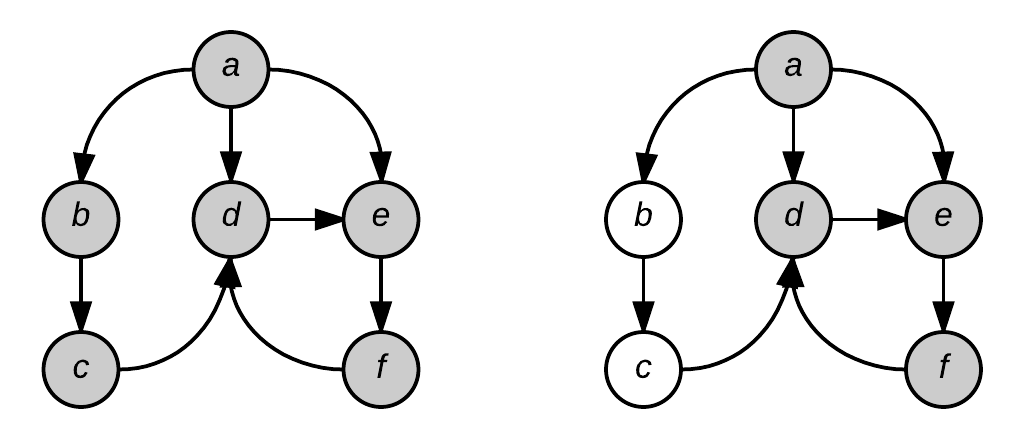
\includegraphics[scale=0.25]{media/chap8/jcharming-slices.png}
\caption{Hypothetical example representing $bslice_{[a \leftarrow d]}$ (left) vs. $\cup_{i=d}^{a} bslice_{[f_{i+1} \leftarrow f_i]}$ (right) for a crash trace $T={d, f, e}$.
\label{fig:jcharming-slice}}
\end{figure}

In the worst case scenario where there exists one and only one
transition between each two frames (this is very unlikely for real and
complex systems) \(bslice_{[entry \leftarrow f_0]}\) and
\(\cup_{i=0}^n bslice_{[f_{i+1} \leftarrow f_i]}\) yield the same set of
states with a comparable computational cost since the number of branches
to explore will be the same in both cases.

Algorithm \ref{alg:jcharming-slice} is a high-level representation of
how we compute the backward slice between each frame. The algorithm
takes as input the preprocessed crash trace
\(T=\{f_0, f_1, f_2, ..., f_N\}\), the byte code of the SUT, and the
entry point. From line 1 to line 4, we initialize the different
variables used by the algorithm. Our algorithm needs to have the crash
trace as an array of frames (line 1), the size \(N\) of the crash trace
(line 2), a \texttt{null} backward static slice (line 4, and an offset
set to 1 (line 3). The main loop of the algorithm begins at line 5 and
ends at line 13. In this loop, we compute the static slice between the
current frame and the next one. If the slice is not empty, then we
update the final backward slice with the newly computed slice. In
Algorithm 1, this is shown as a union between the two slices. Note that
this union preserves the order of the elements of the two slices. This
can also be seen as a concatenation operation. We describe this process
in the subsequent paragraphs through an example. If the computed slice
is empty, it means that Frame \lstinline!i + 1! was corrupted then we
move to Frame \lstinline!i + 2!, and so on. At the end of the algorithm,
we compute the slice between the last frame and the entry point of the
program and update the final slice.

Figure \ref{fig:jcharming-algo} presents a step by step graphical
representation of Algorithm \ref{alg:jcharming-slice}. In this figure,
an hypothetical program, composed of eleven states (\(a...k\)), crashes
at point \(k\). The produced crash trace is composed of six frames
\(T=\{f_0, f_1, f_2, f_3, f_4, f_5\}\). The frames represent \(k\),
\(i\), \(h\), \(d\), \(b\) and \(a\), respectively. In the crash trace,
\(f_3\) is a corrupt frame and no longer matches a location inside the
SUT. This can be the result of a copy-paste error or a deliberate
modification made by the reporter of the bug as shown in the case study
(see Section \ref{sec:results}). In such a situation, Algorithm
\ref{alg:jcharming-slice} will begin by computing the backward static
slice between \(f_0\) (\(k\)) and \(f_1\) (\(i\)), then between \(f_1\)
(\(i\)) and \(f_2\) (\(h\)). At this point, we passed through the
\(for\) loop (lines 5 to 12) two times, and in both cases the backward
static slice was not empty. Consequently, the \(if\) statement was equal
to \(true\) and we combined both backward static slices in the
\(bSlice\) variable. \(bSlice\) is equal to \{\(k\), \(j\), \(i\),
\(h\)\}. Then, we want to compute the backward static slice between
\(f_2\) (\(h\)) and \(f_3\) (\(d\)). Unfortunately, \(f_3\) is corrupted
and does not point towards a valid location in the SUT. As a result, the
slice between \(f_2\) (\(h\)) and \(f_3\) (\(d\)) will be empty, and we
will go to the \(else\) statement (line 10). Here, we simply increment
\(offset\) by one in order to compute the backward static slice from
\(f_2\) (\(h\)) and \(f_4\) (\(b\)) instead of \(f_2\) (\(h\)) and
\(f_3\) (\(d\)). \(f_4\) is valid and the backward static slice from
\(f_2\) (\(h\)) and \(f_4\) (\(b\)) can be computed and merged to
\(bSlice\). Finally, we compute the last slice between \(f_4\) (\(b\))
and \(f_5\) (\(a\)). The final backward static slice is \(k\), \(i\),
\(h\), \(d\), \(b\) and \(a\).

\begin{algorithm}
 \KwData{Crash Stack, BCode, Entry Point}
 \KwResult{BSolve}
 Frame[]~frames $\leftarrow$ extract~frames~from~crash~stack; \\
 Int n $\leftarrow$ size of frames\;
 Int offset $\leftarrow$ 1\;
 Bslice bSlice $\leftarrow$ $\emptyset$\;
\For{i $\leftarrow$ 0; (i $<$ n \&\& offset $<$ n - 1); i++}{
  BSlice currentBSlice $\leftarrow$ backward slice from frames[i] to frames[i + offset]\;
  \eIf{currentBSlice $\not=$ $\emptyset$}{
   bSlice $\leftarrow$ bSlice $\cup$ currentBSlice\;
   offset $\leftarrow$ 1\;
  }{
   offset $\leftarrow$ offset +1\;
  }
}
\caption{High-level algorithm computing the union of the slices\label{alg:jcharming-slice}}
\end{algorithm}

\begin{figure}
  \centering
    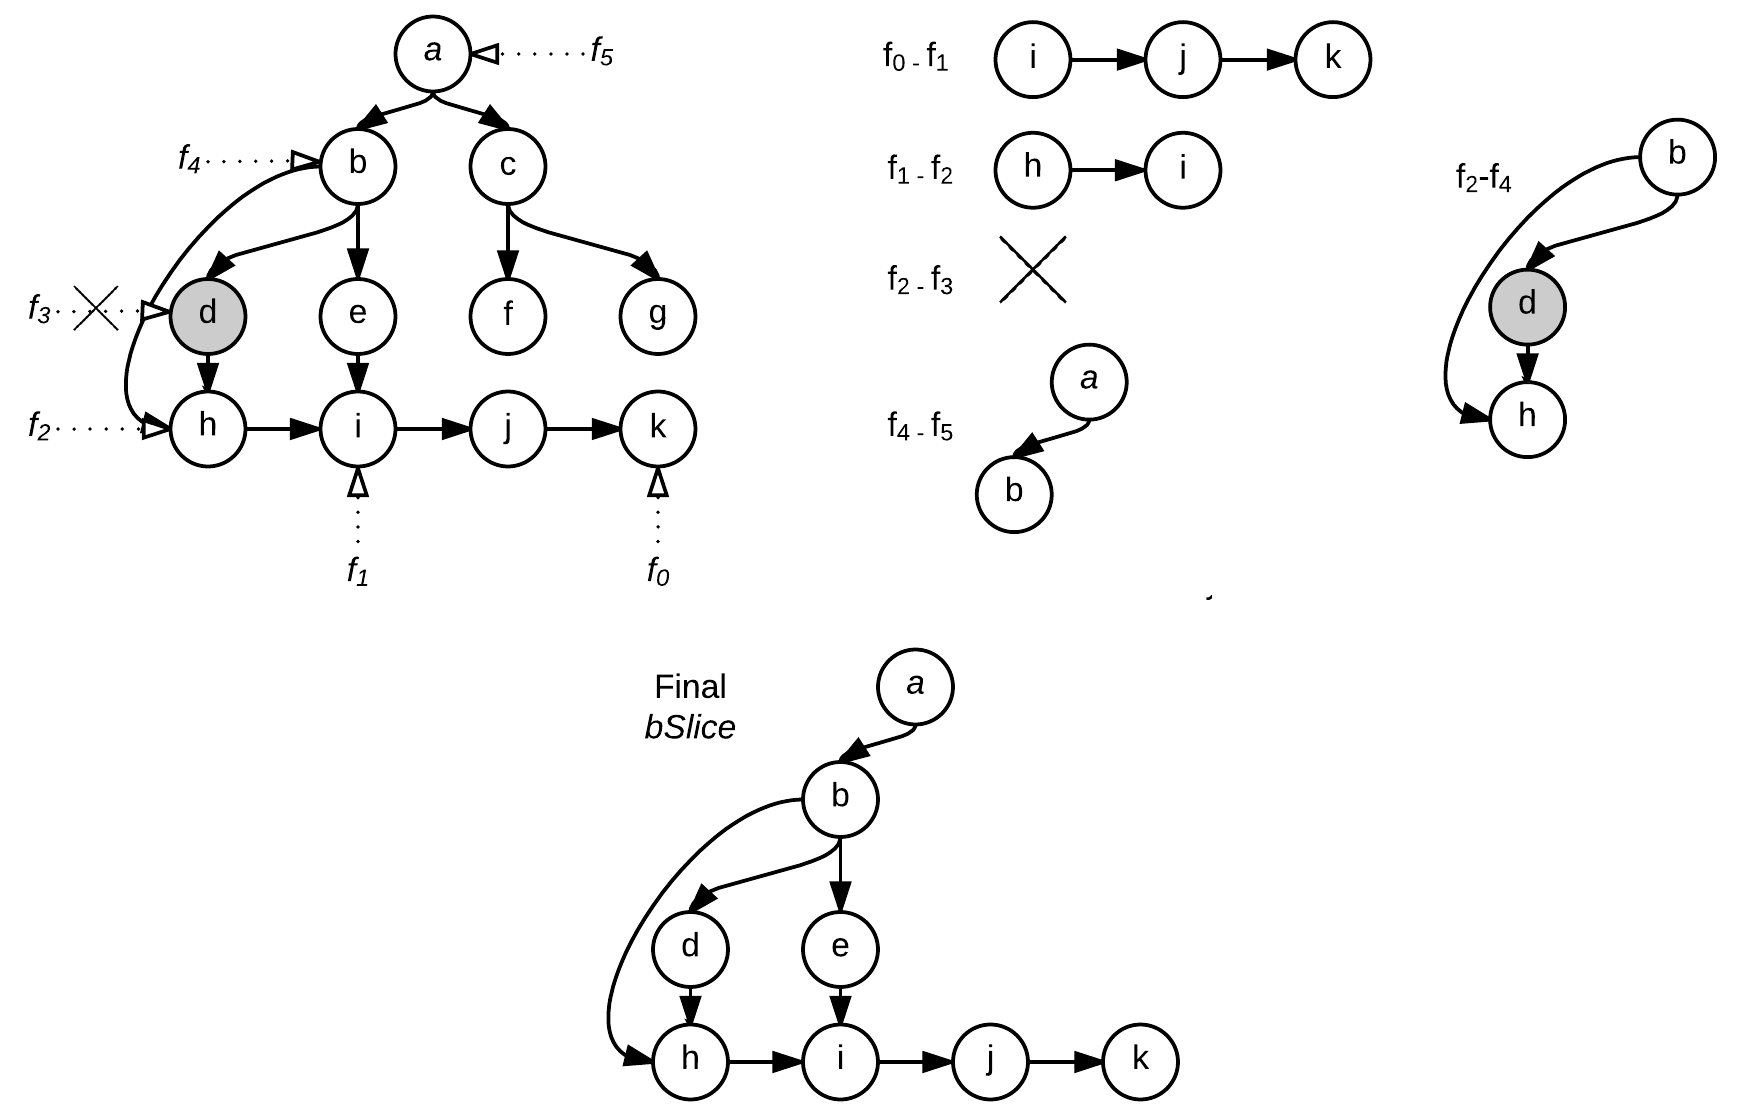
\includegraphics[scale=.20]{media/chap8/algo.png}
    \caption{Steps of Algorithm \ref{alg:jcharming-slice} where $f_3$ is corrupted.
    \label{fig:jcharming-algo}}
\end{figure}

Our algorithm, given an uncorrupted stack trace, will be able to compute
an optimum backward static slice based on the frames (Figure
\ref{fig:jcharming-slice}) and compensate for frames corruption ,if need
be, by \textit{offsetting} the corrupted frame (Figure
\ref{fig:jcharming-algo}). The compensation of corrupted frames,
obviously, comes at the cost of a sub-optimum backward static slice. In
our previous example, the transition between \(b\) and \(h\) could have
been omitted if \(f_3\) was not corrupted.

In the rare cases where the final slice is empty (this may happen in
situations where the content of the crash trace is seriously corrupted)
JCHARMING would simply proceed with non-directed model checking.

Note that while we allow in JCHARMING the possibility to resort to
non-directed model checking, none of the 30 bugs used in this study
contained crash traces that were damaged enough for this fall back
mechanism to be used.

In order to compute the backward slice, we implement our algorithm as an
add-on to the T. J. Watson Libraries for Analysis (WALA) {[}78{]}, which
provide static analysis capabilities for Java Byte code and JavaScript.
WALA offers a very comprehensive API to perform static backward slicing
on Java Byte code from a specific point to another. We did not need to
extend WALA to perform our analysis.

Using backward slicing, the search space of the model checker that
processes the example of Figures \ref{fig:testing-toy} to
\ref{fig:dchecking-toy}, where a crash happens when \(i>2\), is given by
the following expression:

\begin{equation}
Sliced_{SUT} =
\begin{pmatrix}
\bigcup_{i=0}^{entry} bslice_{[f_{i+1} \leftarrow f_i]} \subseteq SUT, \\
S_0, \\
T.\bigcup_{i=0}^{entry} bslice_{[f_{i+1} \leftarrow f_i]}  \subseteq T.SUT, \\
L
\end{pmatrix}
\end{equation}

Where
\(\bigcup_{i=0}^{entry} bslice_{[f_{i+1} \leftarrow f_i]} \subseteq SUT\)
is the subset of states that can be reached in the computed backward
slice, \(S_0\) the set of initial states,
\(T.\bigcup_{i=0}^{entry} bslice_{[f_{i+1} \leftarrow f_i]}\) the subset
of transitions relations between states that exist in the computed
backward slice and \(L\) the labeling function which labels a state with
a set of atomic properties. Then, in the sliced SUT, we try to find:

\begin{equation}
    (Sliced_{SUT}, x) \models p_{i>2}
\end{equation}

That is, there exists a sequence of state transitions \(x\) that
satisfies \(p_{i>2}\). The only frame that needs to be valid for the
backward static slice to be meaningful is \(f_0\). In Figure
\ref{fig:jcarming-traces}, \(f_0\) is \(at~Foo.bar(Foo.java:10)\). If
this line of the crash trace is corrupt, then JCHARMING cannot perform
the slicing because it does not know where to start the backward
slicing. The result is a non-directed model checking, which is likely to
fail.

\subsection{Directed Model Checking}\label{directed-model-checking}

The model checking engine we use in this paper is called JPF (Java
PathFinder) {[}194{]}, which is an extensible JVM for Java byte code
verification. This tool was first created as a front-end for the SPIN
model checker {[}74{]} in 1999 before being open-sourced in 2005. The
JPF model checker can execute all the byte code instructions through a
custom JVM --- known as JVM\textsuperscript{\textit{JPF}}. Furthermore,
JPF is an explicit state model checker, very much like SPIN {[}74{]}.
This is contrasted with a symbolic model checker based on binary
decision diagrams {[}125{]}. JPF designers have opted for a depth-first
traversal with backtracking because of its ability to check for temporal
liveness properties.

More specifically, JPF's core checks for defects that can be checked
without defining any property. These defects are called
\textit{non-functional properties} in JPF and cover deadlock, unhandled
exceptions, and \texttt{assert} expressions. In JCHARMING, we leverage
the \textit{non-functional properties} of JPF as we want to compare the
crash trace produced by unhandled exceptions to the crash trace of the
bug at hand. In other words, we do not need to define any property
ourselves. This said, in JPF, one can define properties by implementing
\texttt{listeners} --- very much like what we did in
Section\textasciitilde{}\ref{sec:unit-tests} --- that can monitor all
actions taken by JPF, which enables the verification of temporal
properties for sequential and concurrent Java programs. One of the
popular \texttt{listeners} of JPF is \texttt{jpf-ltl}. This listener
supports the verification of method invocations or local and global
program variables. \texttt{jpf-ltl} can verify temporal properties of
method call sequences, linear relations between program variables, and
the combination of both. We intend to investigate the use of
\texttt{jpf-ltl} and the LTL logic to check multi-threaded related
crashes as part of future work.

JPF is organized around five simple operations: (i) \emph{generate
states}, (ii) \emph{forward}, (iii) \emph{backtrack}, (iv) \emph{restore
state} and (v) \emph{check}. In the forward operation, the model
checking engine generates the next state \(s_{t+1}\). Each state
consists of three distinct components:

\begin{itemize}
\tightlist
\item
  The information of each thread. More specifically, a stack of frames
  corresponding to method calls.
\item
  The static variables of a given class.
\item
  The instance variables of a given object.
\end{itemize}

If \(s_{t+1}\) has successors, then it is saved in a backtrack table to
be restored later. The backtrack operation consists of restoring the
last state in the backtrack table. The restore operation allows
restoring any state. It can also be used to restore the entire program
as it was the last time we chose between two branches. After each
forward, backtrack and restore state operation the check properties
operation is triggered.

In order to direct JPF, we have to modify the \emph{generate states} and
the \emph{forward} steps. The \emph{generate states} is populated with
the states in
\(\bigcup_{i=0}^{entry} bslice_{[f_{i+1} \leftarrow f_i]} \subset SUT\)
and we adjust the \emph{forward step} to explore a state if the target
state \(s_i+1\) and the transition \(x\) to pass from the current state
\(s_i\) to \(s_{i+1}\) are in
\(\bigcup_{i=0}^{entry} bslice_{[f_{i+1} \leftarrow f_i]} \subset SUT\)
and
\(x.\bigcup_{i=0}^{entry} bslice_{[f_{i+1} \leftarrow f_i]} \subset x.SUT\).

In other words, JPF does not generate each possible state for the system
under test. Instead, JPF generates and explores only the states that
fall inside the backward static slice we computed in the previous step.
As shown in figure \ref{fig:jcharming-slice}, our backward static slice
can greatly reduce the space search and is able to compensate for
corrupted frames. In short, the idea is that instead of going through
all the states of the program as a complete model checker would do, the
backward slice directs the model checker to explore only the states that
might reach the targeted frame.

\subsection{Validation}\label{validation}

To validate the result of directed model checking, we modify the
\emph{check properties} step that checks if the current sequence of
state transition \(x\) satisfies a set of properties. If the current
state transition \(x\) can throw an exception, we execute \(x\) and
compare the exception thrown to the original crash trace (after
preprocessing). If the two exceptions match, we conclude that the
conditions needed to trigger the failure have been met and the bug is
reproduced.

However, as argued by Kim et al. in {[}96{]}, the same failure can be
reached from different paths of the program. Although the states
executed to reach the defect are not exactly the same, they might be
useful to enhance the understanding of the bug by software developers
and speed up the deployment of a fix. Therefore, in this paper, we
consider a defect to be partially reproduced if the crash trace
generated from the model checker matches the original crash trace by a
factor of \(t\), where \(t\) is a threshold specified by the user. The
threshold, \(t\), represents the percentage of identical frames between
both crash traces.

For our experiments (see Section \ref{sec:results}), we set the value of
\(t\) to 80\%. The choice of \(t\) should be guided by the need to find
the best trade-off between the reproducibility of the bug and the
relevance of the generated test cases (the tests should help reproduce
the on-field crash). To determine the best \(t\), we made several
incremental attempts, starting from \(t = 10\%\). For each attempt, we
increased \(t\) with a factor of 5\% and observed the number of bugs
reproduced and the quality of the generated tests. Having \(t = 80\%\)
provided the best trade-off. This said, we anticipate that the tool that
implements our technique should allow software engineers to vary \(t\)
depending on the bugs and the systems under study. Based on our
observations, we recommend, however, to set \(t\) to 80\% as a baseline.
It should also be noted that we deliberately prevented JCHARMING to
perform directed model checking with a threshold below 50\%. This is
because the tests generated with such a low threshold during our
experiments did not yield qualitative results.

\subsection{\texorpdfstring{Generating Test Cases for Bug
Reproduction\label{sec:unit-tests}}{Generating Test Cases for Bug Reproduction}}\label{generating-test-cases-for-bug-reproduction}

To help software developers reproduce the crash in a lab environment, we
automatically produce the JUnit test cases necessary to run the SUT to
cause the bug.

To build a test suite that reproduces a defect, we need to create a set
of objects used as arguments for the methods that will enable us to
travel from the entry point of the program to the defect location. JPF
has the ability to keep track of what happens during model checking in
the form of traces containing the visited states and the value of the
variables. We leverage this capability to create the required objects
and call the methods leading to the failure location.

During the testing of the SUT, JPF emits a trace that is composed of the
executed instructions. For large systems, this trace can contain
millions of instructions. It is stored in memory and therefore can be
queried while JPF is running. However, accessing the trace during the
JPF execution considerably slows down the checking process as both the
querying mechanism and the JPF engine compete with each other for
resources. In order to allow JPF to use 100\% of the available resources
and still be able to query the executed instructions, we implemented a
listener that listens to the JPF trace emitter. Each time JPF processes
a new instruction, our listener catches it and saves it into a MongoDB
database to be queried in a post-mortem fashion. Figure
\ref{fig:jcharming-unittest} presents a high-level architecture of the
components of the JUnit test generation process.

\begin{figure}
  \centering
    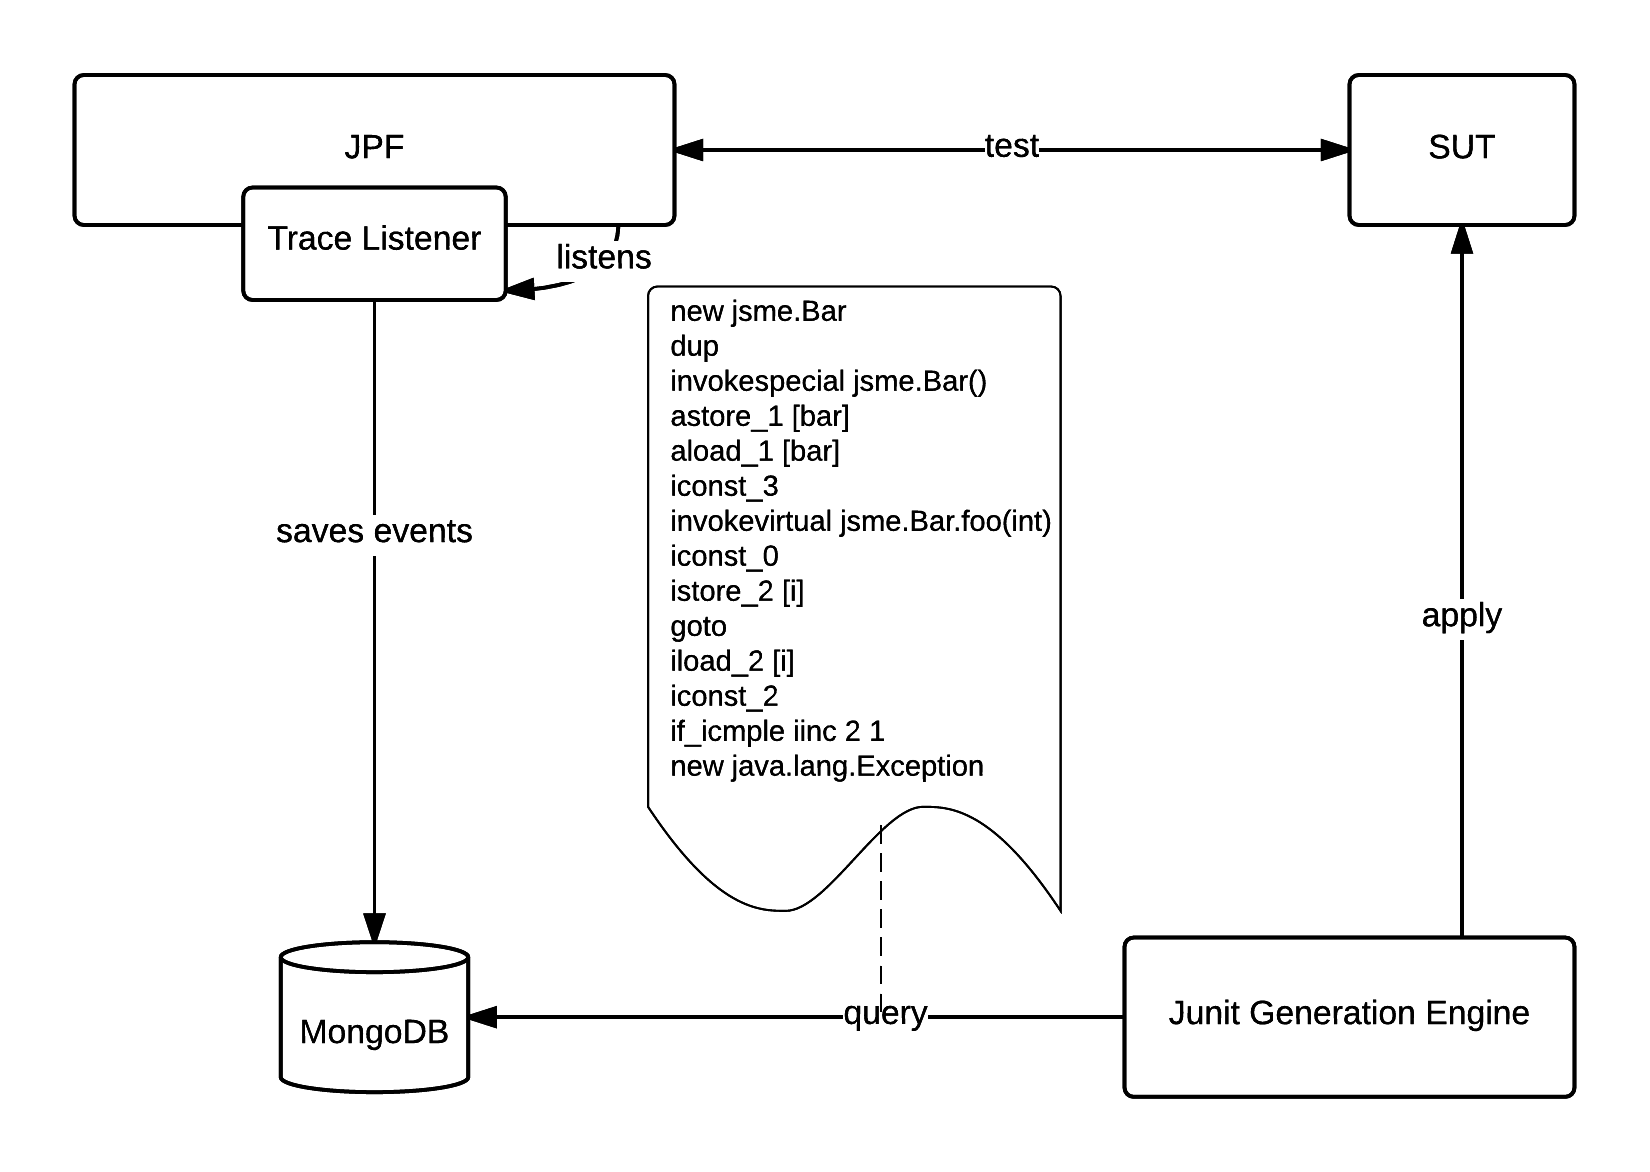
\includegraphics[scale=0.8]{media/chap8/unittest.png}
    \caption{High level architecture of the Junit test case generation
    \label{fig:jcharming-unittest}}
\end{figure}

When the \emph{validate} step triggers a crash stack with a similarity
larger than a factor \emph{t}, the JUnit generation engine queries the
MongoDB database and fetches the sequence of instructions that led to
the crash of interest. Figure \ref{fig:jcharming-unittest} contains a
hypothetical sequence of instructions related to the example of Figures
\ref{fig:testing-toy}, \ref{fig:checking-toy}, \ref{fig:dchecking-toy},
which reads : \emph{new jsme.Bar}, \emph{invokespecial jsme.Bar()},
\emph{astore\_1 {[}bar{]}}, \_aload\_1 {[}bar{]}\emph{,
\emph{iconst\_3}, \emph{invokevirtual jsme.Bar.foo(int)},
\emph{const\_0}, \emph{istore\_2 {[}i{]}}, \emph{goto}, \emph{iload\_2
{[}i{]}}, \emph{iconst\_2}, \emph{if\_icmple iinc 2 1}, \emph{new
java.lang.Exception}. From this sequence we know that, to reproduce to
crash of interest, we have to (1) create a new object \emph{jsme.Bar}
(\emph{new jsme.Bar}, \emph{invokespecial jsme.Bar()}), (2) store the
newly created object in a variable named \emph{bar} (\emph{astore\_1
{[}bar{]}}), (3) invoke the method \emph{jsme.Bar.foo(int)} of the
\emph{bar} object with \emph{3} as value (\emph{aload\_1 {[}bar{]}},
\_iconst\_3}, \emph{invokevirtual jsme.Bar.foo(int)}). Then, the
\emph{jsme.Bar.foo(int)} method will execute the \(for-loop\) from
\(i=0\) until \(i=3\) and throw an exception at \emph{i = 3}
(\emph{const\_0}, \emph{istore\_2 {[}i{]}}, \emph{goto}, \emph{iload\_2
{[}i{]}}, \emph{iconst\_2}, \emph{if\_icmple iinc 2 1}, \emph{new
java.lang.Exception}).

The generation of the JUnit test itself is based on templates and
targets directly the system under test. Templates are excerpts of Java
source code with well-defined tags that will be replaced by values. We
use templates because the JUnit test cases have common structures.
Figure \ref{fig:jcharming-unittemplate} shows our template for
generating JUnit test cases. In this figure, each \emph{\{\% \%\}} will
be dynamically replaced by the corresponding value when the JUnit test
is generated. For example, \emph{\{\% SUT \%\}} will be replaced by
\emph{Ant} if the SUT is Ant. First, we declare four variables that
contain the \emph{failure}, the \emph{threshold} above which a given bug
is said to be partially reproduced, the \emph{differences}, which count
how many lines differ between the original failure, the failure produced
by JCHARMING, and a \emph{StringTokenizer}. The \emph{StringTokenizer}
allows breaking the original \emph{failure} into tokens. Second, the
test method where \emph{\{\%SUT\%\}} is replaced by the name of the SUT
and \emph{\{\%STEPS\%\}} by the steps to make the SUT crash. Then, the
crash trace related to the crash is received in the \emph{catch} part of
the \emph{try-catch} block. In the \emph{catch} part, we compute the
number of lines that do not match the original exception and store it
into \emph{differences}
\footnote{This code has been replaced by $//Count~the~differences$ to ease the reading.}.
Finally, the \emph{assertTrue} call will assert that the crash traces
from the induced and the original crash are at least \emph{threshold}
percent similar to each other.

\begin{figure}[h!]

\noindent\fbox{%
    \parbox{\textwidth}{%
    \lstinputlisting[language=Java]{tex/chap8/test.java}
}%
}
    \caption{Simplified Unit Test template
    \label{fig:jcharming-unittemplate}}
\end{figure}

\section{\texorpdfstring{Experimental
Setup\label{sec:cases}}{Experimental Setup}}\label{experimental-setup-3}

In this section, we show the effectiveness of JCHARMING to reproduce
bugs in ten open source systems. The case studies aim to answer the
following question: \emph{Can we use crash traces and directed model
checking to reproduce on- field bugs in a reasonable amount of time?}

\subsection{Targeted Systems}\label{targeted-systems}

Table \ref{tab:jacharming-systems} shows the systems and their
characteristics in terms of Kilo Line of Code (KLoC) and Number of
Classes (NoC).

\begin{table}
\centering

\caption{List of target systems in terms of Kilo line of code (KLoC), number of classes (NoC) and Bug \# ID}
\begin{tabular}{c|c|c|c}
SUT        & KLOC & NoC  & Bug \#ID                                        \\ \hline \hline
Ant        & 265  & 1,233 & 38622, 41422                                    \\
ArgoUML    & 58   & 1,922 & 2603, 2558, 311, 1786                           \\
dnsjava    & 33   & 182  & 38                                              \\
jfreechart & 310  & 990  & 434, 664, 916                                   \\
Log4j      & 70   & 363  & 11570, 40212, 41186, 45335, 46271, 47912, 47957 \\
MCT        & 203  & 1267 & 440ed48                                         \\
pdfbox     & 201  & 957  & 1,412, 1,359 \\
Hadoop     & 308   & 6,337 & 2893, 3093, 11878\\
Mahout     & 287  & 1,242 &  486, 1367, 1594, 1635\\
ActiveMQ   & 205  & 3,797 & 1054, 2880, 2880\\ \hline
Total      & 1,517 & 17,348 & 30 \\
\hline \hline
\end{tabular}
\label{tab:jacharming-systems}
\end{table}

Apache Ant {[}4{]} is a popular command-line tool to build Makefiles.
While it is mainly known for Java applications, Apache Ant also allows
building C and C++ applications. We choose to analyze Apache Ant because
other researchers in similar studies have used it.

ArgoUML {[}37{]} is one of the major players among the open source UML
modeling tools. It has many years of bug management and, similar to
Apache Ant, it has been extensively used as a test subject in many
studies.

Dnsjava {[}199{]} is a tool for the implementation of the DNS mechanisms
in Java. This tool can be used for queries, zone transfers, and dynamic
updates. It is not as large as the other two, but it still makes an
interesting case subject because it has been well maintained for the
past decade. Also, this tool is used in many other popular tools such as
Aspirin, Muffin and Scarab.

JfreeChart {[}149{]} is a well-known library that enables the creation
of professional charts. Similar to dnsjava, it has been maintained over
a very long period of time. JfreeChart was created in 2005. It is a
relatively large application.

Apache Log4j {[}184{]} is a logging library for Java. This is not a very
large library, but thousands of programs extensively use it. As other
Apache projects, this tool is well maintained by a strong open source
community and allows developers to submit bugs. The bugs that are in the
bug reporting system of Log4j are generally well documented. In
addition, the majority of bugs contain crash traces, which makes Log4j a
good candidate system for this study.

MCT {[}134{]} stands for Mission Control technologies and was developed
by the NASA Ames Research Center (the creators of JPF) for use in
spaceflight mission operation. This tool benefits from two years of
history and targets a very critical domain, Spacial Mission Control.
Therefore, this tool has to be particularly and carefully tested and,
consequently, the remaining bugs should be hard to discover and
reproduce.

PDFBox {[}5{]} is another tool supported by the Apache Software
Foundation since 2009 and was created in 2008. PDFBox allows the
creation of new PDF documents and the manipulation of existing
documents.

Hadoop {[}7{]} is a framework for storing and processing large datasets
in a distributed environment. It contains four main modules:
\emph{Common}, \emph{HDFS}, \emph{YARN} and \emph{MapReduce}. In this
paper, we study the \emph{Common} module that contains the different
libraries required by the other three modules.

Mahout {[}8{]} is a relatively new software application, built on top of
Hadoop. We used Mahout version 0.11, which was released in August 2015.
Mahout supports various machine learning algorithms with a focus on
collaborative filtering, clustering, and classification.

Finally, ActiveMQ {[}174{]} is an open source messaging server that
allows applications written in Java, C, C++, C\#, Ruby, Perl or PHP to
exchange messages using various protocols. ActiveMQ has been actively
maintained since it became an Apache Software Foundation project in
2005.

\begin{table}[]
\centering
\caption{Effectiveness of JCHARMING using directed model checking (DMC) in minutes, length of the generated JUnit tests (CE length) and model checking (MC) in minutes}
\begin{tabular}{c|c|c|c|c|c}
SUT                         & Bug \#ID & Reprod. & Time DMC & CE length & Time MC \\ \hline \hline
\multirow{2}{*}{Ant}        & 38622    & Yes     & 25.4   & 3  & -       \\
                            & 41422    & No      & 42.3   & -  & -       \\ \hline
\multirow{4}{*}{ArgoUML}    & 2558     & Partial & 10.6   & 3  & -       \\
                            & 2603     & Partial & 9.4    & 3  & -       \\
                            & 311      & Yes     & 11.3   & 10  & -       \\
                            & 1786     & Partial & 9.9    & 6  & -       \\  \hline
DnsJava                     & 38       & Yes     & 4      & 2  & 23      \\ \hline
\multirow{3}{*}{jFreeChart} & 434      & Yes     & 27.3   & 2  & -       \\
                            & 664      & Partial & 31.2   & 3   & -       \\
                            & 916      & Yes     & 26.4   & 4  & -       \\ \hline
\multirow{7}{*}{Log4j}      & 11570    & Yes     & 12.1   & 2  & -       \\
                            & 40212    & Yes     & 15.8   & 3  & -       \\
                            & 41186    & Partial & 16.7   & 9  & -       \\
                            & 45335    & No      & 3.2    & -  & -       \\
                            & 46271    & Yes     & 13.9   & 4  & -       \\
                            & 47912    & Yes     & 12.3   & 3  & -       \\
                            & 47957    & No      & 2      & -  & -       \\ \hline
MCT                         & 440ed48  & Yes     & 18.6   & 3  & -       \\ \hline
\multirow{2}{*}{PDFBox}     & 1412     & Partial & 19.7   & 4  & -       \\
                            & 1359     & No      & 7.5    & -    & - \\ \hline
\multirow{4}{*}{Mahout}     & 486      & Partial & 34.5   & 5    & -        \\
                            & 1367     & Partial & 21.1   & 7  & -       \\
                            & 1594     & No      & 14.8       & -  & -       \\
                            & 1635     & Yes     & 31.0   & 14  & - \\ \hline
\multirow{3}{*}{Hadoop}     & 2893     & Partial & 7.4    & 3  & 32       \\
                            & 3093      & Yes      & 13.1     & 2     & -   \\
                            & 11878    & Yes     & 17.4     & 6 & - \\  \hline
\multirow{3}{*}{ActiveMQ}   & 1054     & Yes     & 38.3   & 11  & -      \\
                            & 2880      & Partial  & 27.4    & 6    & -       \\
                            & 5035     & No      & 1  & -  & - \\  \hline \hline
\end{tabular}


\label{tab:jcharming-results}
\end{table}

\subsection{Bug Selection and Crash
Traces}\label{bug-selection-and-crash-traces}

In this study, we have selected the reproduced bugs randomly in order to
avoid the introduction of any bias. We selected a random number of bugs
ranging from 1 to 10 for each SUT containing the word ``exception'' and
where the description of the bug contains a match to a regular
expression designed to find the pattern of a Java exception.

\section{\texorpdfstring{Empirical
Validation\label{sec:results}}{Empirical Validation}}\label{empirical-validation-3}

Table \ref{tab:jcharming-results} shows the results of JCHARMING in
terms of Bug \#ID, reproduction status, and execution time (in minutes)
of directed model checking (DMC), length of the counter-example
(statements in the JUnit test), and execution time (in minutes) for
Model Checking (MC). The experiments have been conducted on a Linux
machine (8 GB of RAM and using Java 1.7.0\_51).

\begin{itemize}
\tightlist
\item
  The result is noted as ``Yes'' if the bug has been fully reproduced,
  meaning that the crash trace generated by the model checker is
  identical to the crash trace collected during the failure of the
  system.
\item
  The result is ``Partial'' if the similarity between the crash trace
  generated by the model checker and the original crash trace is above
  t=80\% and below t=100\%. Given an 80\% similarity threshold, we
  consider partial reproduction as successful. A different threshold
  could be used.
\item
  Finally, the result of the approach is reported as ``No'' if either
  the similarity is below \(t < 80\%\) or the model checker failed to
  crash the system given the input we provided.
\end{itemize}

As we can see in Table \ref{tab:jcharming-results}, we were able to
reproduce 24 out of 30 bugs either completely or partially (80\% success
ratio). The average time to reproduce a bug was 19 minutes. The average
time in cases where JCHARMING failed to reproduce the bug was 11
minutes. The maximum fail time was 42.3 minutes, which was the time
required for JCHARMING to fill all the available memory and stop and a
\(-\) denotes that JCHARMING reached a sixty-minute timeout. Finally, we
report the number of statements in the produced JUnit test, which
represents the length of the counter-example. While reproducing a bug is
the first step in understanding the cause of a field crash, the steps to
reproduce the bug should be as few as possible. It is important for
counter-examples to be short to help the developers provide a fix
effectively. In average, JCHARMING counter-examples were composed of
5.04 Java statements, which, in our view, is considered reasonable for
our approach to be adopted by software developers. This result
demonstrates the effectiveness of our approach, more particularly, the
use of backward slicing to create a manageable search space that guides
the model checking engine adequately. We also demonstrated that our
approach is usable in practice since it is also time efficient. Among
the 30 different bugs we have tested, we will describe two bugs (chosen
randomly) for each category (successfully reproduced, partially
reproduced, and not reproduced) for further analysis. The bug report
presented in the following sections are the original reports as
submitted by the reporter. As such, they contain typos and spelling
mistakes that we did not correct.

\subsection{Successfully Reproduced}\label{successfully-reproduced}

The first bug we describe in this discussion is the bug \#311 belonging
to ArgoUML. This bug was submitted in an earlier version of ArgoUML.
This bug is very simple to manually reproduce thanks to the extensive
description provided by the reporter, which reads: \emph{I open my first
project (Untitled Model by default). I choose to draw a Class Diagram. I
add a class to the diagram. The class name appears in the left browser
panel. I can select the class by clicking on its name. I add an instance
variable to the class. The attribute name appears in the left browser
panel. I can't select the attribute by clicking on its name. Exception
occurred during event dispatching:} The reporter also attached the crash
trace presented in Figure \ref{fig:argo} that we used as input for
JCHARMING:

\begin{figure}[]
\noindent\fbox{%
    \parbox{\textwidth}{%
1. java.lang.NullPointerException:\\
2. at\\
3. uci.uml.ui.props.PropPanelAttribute
.setTargetInternal (PropPanelAttribute.java)\\
4. at uci.uml.ui.props.PropPanel.
setTarget(PropPanel.java)\\
5. at uci.uml.ui.TabProps.setTarget(TabProps.java)\\
6. at uci.uml.ui.DetailsPane.setTarget
(DetailsPane.java)\\
7. at uci.uml.ui.ProjectBrowser.select
(ProjectBrowser.java)\\
8. at uci.uml.ui.NavigatorPane.mySingleClick
(NavigatorPane.java)\\
9. at uci.uml.ui.NavigatorPane\$Navigator
MouseListener.mouse Clicked(NavigatorPane.java)\\
10.at
java.awt.AWTEventMulticaster.mouseClicked
(AWTEventMulticaster.java:211)\\
11.
at
java.awt.AWTEventMulticaster.mouseClicked
(AWTEvent
Multicast er.java:210)\\
12.at
java.awt.Component.processMouseEvent
(Component.java:3168)\\
...\\
19. java.awt.LightweightDispatcher
.retargetMouseEvent (Container.java:2068)\\
22.
at java.awt.Container
.dispatchEventImp l(Container.java:1046)\\
23.
at java.awt.Window
.dispatchEventImpl (Window.java:749)\\
24.
at java.awt.Component
.dispatchEvent (Component.java:2312)\\
25.
at java.awt.EventQueue
.dispatchEvent (EventQueue.java:301)\\
28.
at java.awt.EventDispatchThread.pumpEvents\\
(EventDispatch Thread.java:90) \\
29.
at java.awt.EventDispatchThread.run(EventDispatch
Thread.java:82)
    }%
}
\caption{Crash trace reported for bug ArgoUML \#311\label{fig:argo}}
\end{figure}

The cause of this bug is that the reference to the attribute of the
class was lost after being displayed on the left panel of ArgoUML and
therefore, selecting it through a mouse click throws a null pointer
exception. In the subsequent version, ArgoUML developers added a
TargetManager to keep the reference of such object in the program. Using
the crash trace, JCHARMING's preprocessing step removed the lines
between lines 11 and 29 because they belong to the Java standard library
and we do not want either the static slice or the model checking engine
to verify the Java standard library but only the SUT. Then, the third
step performs the static analysis following the process described in
Section IV.C. The fourth step performs the model checking on the static
slice to produce the same crash trace. More specifically, the model
checker identifies that the method \emph{setTargetInternal(Object o)}
could receive a null object that will result in a \emph{Null} pointer
exception.

The second reproduced bug we describe in this section is Bug \#486
belonging to MAHOUT. The submitter (Robin Anil) named the bug entry as
\emph{Null Pointer Exception running DictionaryVectorizer with ngram=2
on Reuters dataset}. He simply copied the crash stack presented in
Figure \ref{fig:mahout} without further explanation.

\begin{figure}[]

\noindent\fbox{%
    \parbox{\textwidth}{%
1 java.io.IOException: Spill failed \\
2 at org.apache.hadoop.mapred.MapTask\$MapOutputBuffer.collect \\ (MapTask.java:860) \\
...\\
14 Caused by: java.lang.NullPointerException \\
15 at java.io.ByteArrayOutputStream.write(ByteArrayOutputStream.java:86) \\
16 at java.io.DataOutputStream.write(DataOutputStream.java:90) \\
17 at org.apache.mahout.utils.nlp.collocations.llr.Gram.write(Gram.java:181) \\
18 at org.apache.hadoop.io.serializer.WritableSerialization\$WritableSerializer.serialize ... \\
19 at org.apache.hadoop.io.serializer.WritableSerialization\$WritableSerializer.serialize ... \\
20 at org.apache.hadoop.mapred.IFile\$Writer.append(IFile.java:179) \\
21 at org.apache.hadoop.mapred.Task\$CombineOutputCollector.collect \\ (Task.java:880) \\
22 at org.apache.hadoop.mapred.Task\$NewCombinerRunner\$OutputConverter.write ... \\
23 at org.apache.hadoop.mapreduce.TaskInputOutputContext.write ... \\
24 at org.apache.mahout.utils.nlp.collocations.llr.CollocCombiner \\ .reduce(CollocCombiner.java:40) \\
25 at org.apache.mahout.utils.nlp.collocations.llr.CollocCombiner \\ .reduce(CollocCombiner.java:25) \\
26 at org.apache.hadoop.mapreduce.Reducer.run(Reducer.java:176) \\
27 at org.apache.hadoop.mapred.Task\$NewCombinerRunner.combine(Task.java:1222) \\
28 at org.apache.hadoop.mapred.MapTask\$MapOutputBuffer.\\ sortAndSpill(MapTask.java:1265) \\
29 at org.apache.hadoop.mapred.MapTask\$MapOutputBuffer.\\ access\$1800(MapTask.java:686) \\
30 at org.apache.hadoop.mapred.MapTask\$MapOutputBuffer \\ \$SpillThread.run(MapTask.java:1173) \\
}%
}

\caption{Crash trace reported for bug Mahout \#486\label{fig:mahout}}
\end{figure}

Drew Farris\footnote{https://issues.apache.org/jira/browse/MAHOUT-486},
who was assigned to fix this bug, commented \emph{Looks like this was
due to an improper use of the Gram default constructor that happened as
a part of the
0.20.2\footnote{Farris certainly meant 0.10.2 which was the last refactor of the incriminated class, and the current version of Mahout is 0.11}
refactoring work.} While this quick comment, made only two and a half
hours after the bug submission, was insightful as shown in our generated
test
case\footnote{As a reminder, the generated test cases are made available at research.mathieu-nayrolles.com/jcharming},
the fix happened in the \emph{CollocCombiner} class that is one of the
\emph{Reducer}\footnote{As in Map/Reduce} available in Mahout. The fix
(commit \#f13833) involved creating an iterator to combine the
frequencies of the \emph{Gram} and a null check of the final frequency.

JCHARMING's preprocessing step removed the lines between lines 1 to 14
because they belong to the second thrown exception since
\emph{java.lang.NullPointerException} occurred when writing in a
\emph{ByteArrayOutputStream}. JCHARMING aims to reproduce the root
exceptions and not the exceptions that derive from other exceptions.
This said, the \emph{java.io.IOException: Spill failed} was ignored, and
our directed model checking engine focused, with success, on reproducing
the \emph{java.lang.NullPointerException}.

\subsection{Partially Reproduced}\label{partially-reproduced}

As an example of a partially reproduced bug, we explore Bug \#664 of the
Jfreechart program. The description provided by the reporter is:
\emph{In ChartPanel.mouseMoved there's a line of code which creates a
new ChartMouseEvent using as first parameter the object returned by
getChart(). For getChart() is legal to return null if the chart is null,
but ChartMouseEvent's constructor calls the parent constructor which
throws an IllegalArgumentException if the object passed in is null.}

The reporter provided the crash trace containing 42 lines and then
replaced an unknown number of lines by the following statement
\emph{\textless{}\$deleted entry\$\textgreater{}}. While JCHARMING
successfully reproduced a crash yielding almost the same trace as the
original trace, the \emph{\textless{}\$deleted entry\$\textgreater{}}
statement -- which was surrounded by calls to the standard Java library
-- was not suppressed and stayed in the crash trace. That is, JCHARMING
produced only the 6 (out of 7) first lines and reached 83\% similarity,
and thus a partial reproduction.

\begin{figure}[]

\noindent\fbox{%
    \parbox{\textwidth}{%

1. java.lang.IllegalArgumentException: null source\\
2. at java.util.EventObject.<init>(
EventObject.java:38)\\
3. at\\
4 org.jfree.chart.ChartMouseEvent.<init>
(ChartMouseEvent.java:83)\\
5. at org.jfree.chart.ChartPanel
.mouseMoved(ChartPanel.java:1692)\\
6. $<$deleted entry$>$

    }%
}

\caption{Crash trace reported for bug JFreeChart \#664\label{fig:jfree}}
\end{figure}

The second partially reproduced bug we present here is Bug \#2893
belonging to Hadoop. This bug, reported in February 2008 by Lohit
Vijayarenu, was titled \emph{checksum exceptions on trunk} and contained
the following description: \emph{While running jobs like Sort/WordCount
on trunk I see few task failures with ChecksumException. Re-running the
tasks on different nodes succeeds. Here is the stack}

\begin{lstlisting}[language=Java]
1 Map output lost, rescheduling: getMapOutput(task_200802251721_0004_m_000237_0,29) failed : 
2 org.apache.hadoop.fs.ChecksumException: Checksum error: /tmps/4/apred-tt/mapred-local/task_200802251721_0004_m_000237_0/file.out at 2085376 
3 at org.apache.hadoop.fs.FSInputChecker.verifySum(FSInputChecker.java:276) 
4 at org.apache.hadoop.fs.FSInputChecker.readChecksumChunk(FSInputChecker.java:238) 
5 at org.apache.hadoop.fs.FSInputChecker.read1(FSInputChecker.java:189) 
6 at org.apache.hadoop.fs.FSInputChecker.read(FSInputChecker.java:157) 
7 at java.io.DataInputStream.read(DataInputStream.java:132) 
8 at org.apache.hadoop.mapred.TaskTracker$MapOutputServlet.doGet(TaskTracker.java:2299) 
...
23 at org.mortbay.util.ThreadPool$PoolThread.run(ThreadPool.java:534)
\end{lstlisting}

Similarly to the first partially reproduced bug, the crash traces
produced by our directed model checking engine and the related test case
did not match 100\% of the attached crash stack. While JCHARMING
successfully reproduced the bug, the crash stack contains timestamps
information (e.g., 200802251721), that was logically different in our
produced stack trace as we ran the experiment years later.

In all bugs that were partially reproduced, we found that the
differences between the crash trace generated from the model checker and
the original crash trace (after preprocessing) consist of a few lines
only.

\subsection{Not Reproduced}\label{not-reproduced}

To conclude the discussion on the case study, we present a case where
JCHARMING was unable to reproduce the failure. For the bug \#47957,
belonging to LOG4J and reported in late 2009 the author wrote:
\emph{Configure SyslogAppender with a Layout class that does not exist;
it throws a NullPointerException. Following is the exception trace:} and
attached the following crash trace:

\begin{lstlisting}[language=Java]
1. 10052009 01:36:46 ERROR [Default: 1]
struts.CPExceptionHandler.execute
RID[(null;25KbxlK0voima4h00ZLBQFC;236Al8E60000045C3A
7D74272C4B4A61)] 
2. Wrapping Exception in ModuleException
3. java.lang.NullPointerException
4. at org.apache.log4j.net.SyslogAppender
.append(SyslogAppender.java:250)
5. at org.apache.log4j.AppenderSkeleton
.doAppend(AppenderSkeleton.java:230)
6. at org.apache.log4j.helper.AppenderAttachableImpl
.appendLoopOnAppenders(AppenderAttachableImpl
.java:65)
7. at org.apache.log4j.Category.callAppenders
(Category.java:203)
8. at org.apache.log4j.Category
.forcedLog(Category.java:388)
9. at org.apache.log4j.Category.info
(Category.java:663)
\end{lstlisting}

The first three lines are not produced by the standard execution of the
SUT but by an ExceptionHandler belonging to Struts {[}6{]}. Struts is an
open source MVC (Model View Controller) framework for building Java web
applications. JCHARMING examined the source code of Log4J for the crash
location \emph{struts.CPExceptionHandler.execute} and did not find it
since this method belongs to the source base of Struts -- which uses
log4j as a logging mechanism. As a result, the backward slice was not
produced, and we failed to perform the next steps. It is noteworthy that
the bug is marked as a duplicate of the bug \#46271 which contains a
proper crash trace. We believe that JCHARMING could have successfully
reproduced the crash if it was applied to the original bug.

The second bug that we did not reproduce and that we present in this
section belongs to Mahout. Jaehoon Ko reported it on July 2014. Bug
\#1594 is titled \emph{Example factorize-movielens-1M.sh does not use
HDFS} and reads \emph{It seems that factorize-movielens-1M.sh does not
use HDFS at all. All paths look local paths, not HDFS. So the example
crashes because it cannot find input data from HDFS:}

\begin{lstlisting}[language=Java]
1 Exception in thread $$main'' org.apache.hadoop.mapreduce.lib.input.InvalidInputException: Input path does not exist: /tmp/mahout-work-hoseog.lee/movielens/ratings.csv 
2 at org.apache.hadoop.mapreduce.lib.input.FileInputFormat.singleThreadedListStatus ... 
3 at org.apache.hadoop.mapreduce.lib.input.FileInputFormat.listStatus ... 
... 
31 at org.apache.hadoop.util.RunJarm.theain(RunJar.java:212)
\end{lstlisting}

This entry was marked as \emph{Not A Problem / WONT\_FIX} meaning that
the reported bug was not a bug in the first place. The resolution of
this
bug\footnote{https://github.com/apache/mahout/pull/38\#issuecomment-51436303}
involved the modification of a bash script that Ko (the submitter) was
using to \emph{query} Mahout. In other words, the cause of the failure
was external to Mahout itself, and this is why JCHARMING could not
reproduce it.

\section{\texorpdfstring{Threats to
Validity\label{sec:threats}}{Threats to Validity}}\label{threats-to-validity-4}

The selection of SUTs is one of the common threats to validity for
approaches aiming to improve the understanding of a program's behavior.
It is possible that the selected programs share common properties that
we are not aware of and therefore, invalidate our results. However, the
SUTs analyzed by JCHARMING are the same as the ones used in similar
studies. Moreover, the SUTs vary in terms of purpose, size and history.

Another threat to validity lies in the way we have selected the bugs
used in this study. We selected the bugs randomly to avoid any bias. One
may argue that a better approach would be to select bugs based on
complexity or other criteria (severity, etc.). We believe that a complex
bug (if complexity can at all be measured) may perhaps have an impact on
the running time of the approach, but we are not convinced that the
accuracy of our approach depends on the complexity or the type of bugs
we use. Instead, it depends on the quality of the produced crash trace.
This said, in theory, we may face situations where the crash trace is
completely corrupted. In such cases, there is nothing that guides the
model checker. In other words, we will end up running a full model
checker. It is difficult to evaluate the number of times we may face
this situation without conducting an empirical study on the quality of
crash traces. We defer this to future work.

In addition, we see a threat to validity that stems from the fact that
we only used open source systems. The results may not be generalizable
to industrial systems.

Field failures can also occur due to the running environment in which
the program is executed. For instance, the failure may have been caused
by the reception of a network packet or the opening of a given file
located on the hard drive of the users. The resulting failures will
hardly be reproducible by JCHARMING.

Finally, the programs we used in this study are all written in the Java
programming language and JCHARMING leverages the crash traces produced
by the JVM to reproduce bugs. This can limit the generalization of the
results. However, similar to Java, .Net, Python and Ruby languages also
produce crash traces. Therefore, JCHARMING could be applied to other
object-oriented languages.

In conclusion, internal and external validity have both been minimised
by choosing a relatively large set of different systems and using input
data that can be found in other programming languages.

\section{\texorpdfstring{Chapter
Summary\label{sec:conclusion}}{Chapter Summary}}\label{chapter-summary-4}

In this chapter, we presented JCHARMING (Java CrasH Automatic
Reproduction by directed Model checking), an automatic bug reproduction
technique that combines crash traces and directed model checking.
JCHARMING relies on crash traces and backward program slices to direct a
model checker. This way, we do not need to visit all the states of the
subject program, which would be computationally taxing. When applied to
thirty bugs from ten open source systems, JCHARMING was able to
successfully reproduce 80\% of the bugs. The average time to reproduce a
bug was 19 minutes, which is quite reasonable, given the complexity of
reproducing bugs that cause field crashes.

This said, JCHARMING suffers from three main limitations. The first one
is that it cannot reproduce bugs caused by multi-threading. We
can overcome this limitation by using advanced features of the JPF model
checker such as the \emph{jpf-ltl} listener. The \emph{jpf-ltl} listener
was designed to check temporal properties of concurrent Java programs.
The second limitation is that JCHARMING cannot be used if external
inputs cause the bug. We can always build a monitoring system to
retrieve this data, but this may lead to privacy concerns. Finally, the
third limitation is that the performance of JCHARMING relies on the
quality of the crash traces. This limitation can be addressed by
investigating techniques that can improve the reporting of crash traces.
For the time being, the bug reporters simply copy and paste (and modify)
the crash traces into the bug description. A better practice would be to
automatically append the crash trace to the bug report, for example, in
a different field than the bug description.


\chapter{Towards a Classification of Bugs Based on the Location of the
Corrections: An Empirical
Study}\label{towards-a-classification-of-bugs-based-on-the-location-of-the-corrections-an-empirical-study}

\section{Introduction}\label{introduction-5}

In previous chapters, we showed how to prevent clones and
defects at commit-time, and reproduce on-field crashes.

These techniques, however, treat all bugs as the same.  This is also the case for other studies in the literature (e.g., {[}198, 212{]}). For example, a bug that requires only one fix is analyzed the same way as a bug that necessitates multiple fixes. Similarly, if multiple bugs are fixed by modifying the exact same locations in the code, then we should investigate how these bugs are related in order to predict them in the future. Note here that we do not refer to duplicate bugs. Duplicate bugs are marked as duplicate (and not fixed) and only the master bug is fixed.

[Wahab: I think you should put the example we have in the SQUADE paper]

With this in mind, the relationship between bugs and fixes can be
modelled using the UML diagram in Figure \ref{fig:bug-taxo-diag}. The
diagram only includes bug reports that are fixed and not, for example,
duplicate reports. From this figure, we can think of four instances of
this diagram, which we refer to as bug taxonomy or simply bug types (see
Figure \ref{fig:bug-taxo}).

\begin{figure}[h!]
  \centering
    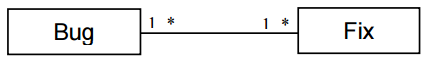
\includegraphics[scale=0.5]{media/chap9/bug-taxo-class-diag.png}
    \caption{Class diagram showing the relationship between bugs and fixed
    \label{fig:bug-taxo-diag}}
\end{figure}

\begin{figure}[h!]
  \centering
    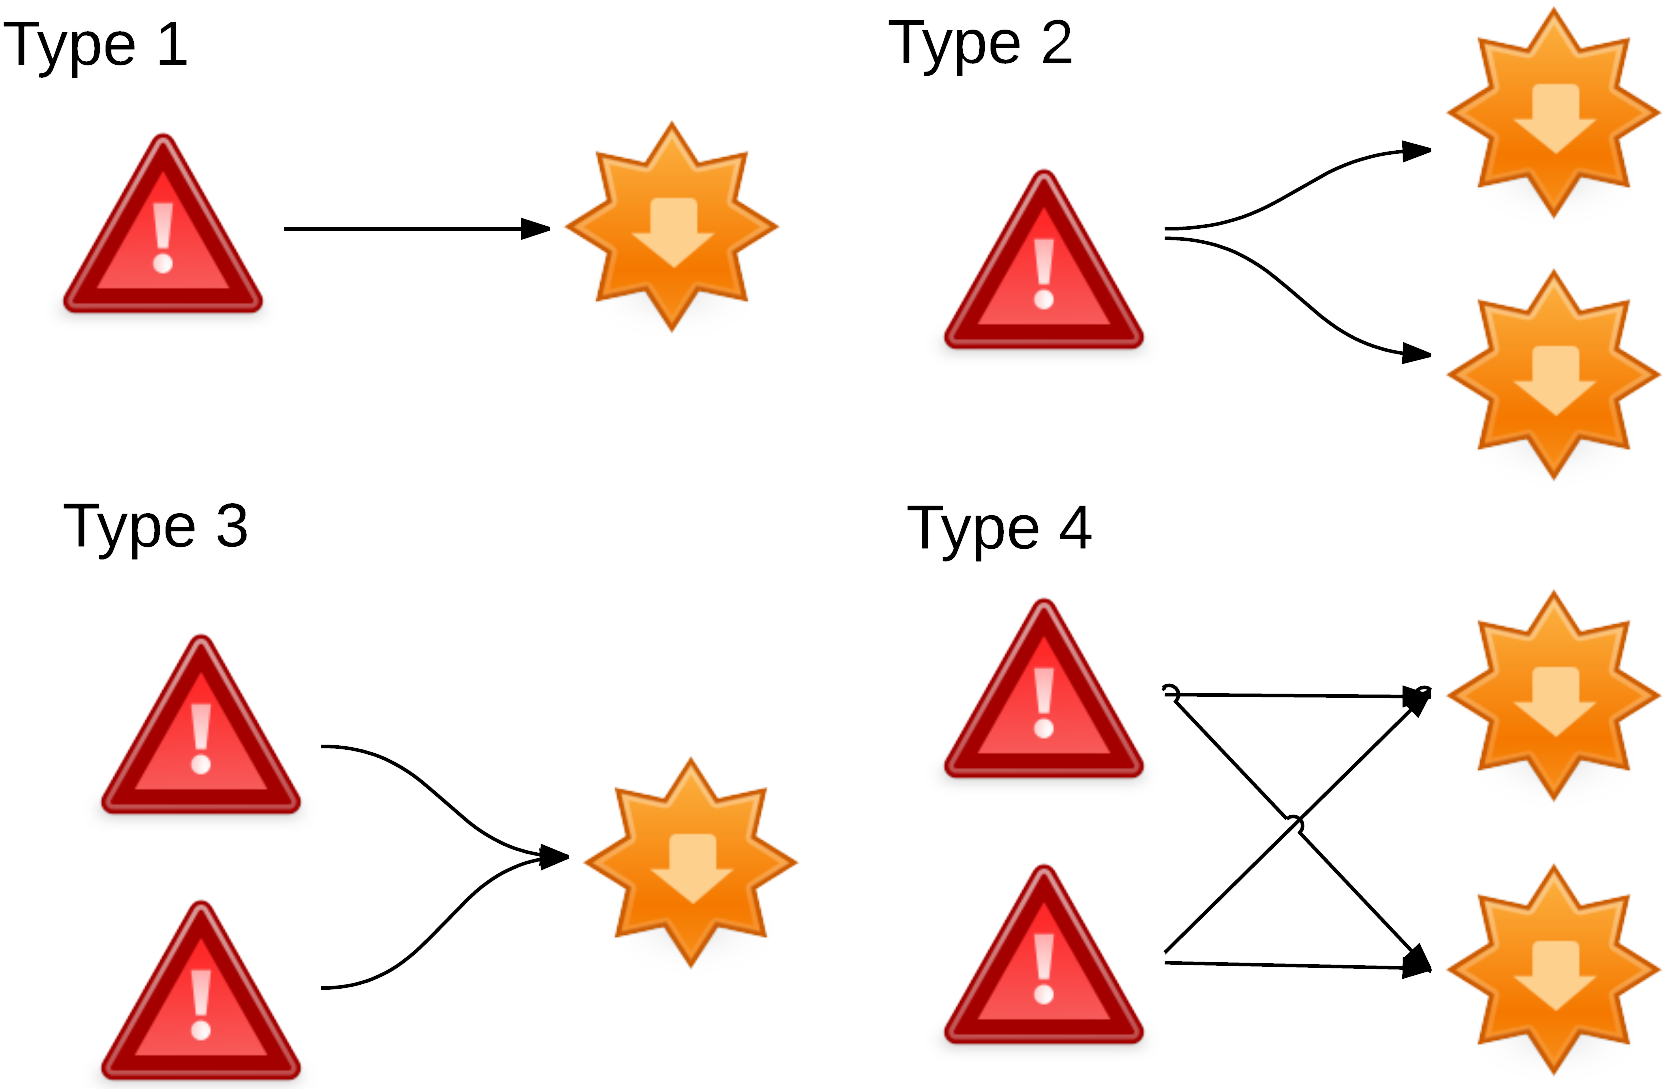
\includegraphics[scale=0.6]{media/chap9/bug-taxo.png}
    \caption{Proposed Taxonomy of Bugs
    \label{fig:bug-taxo}}
\end{figure}

The first and second types are the ones we intuitively know about. T1
refers to a bug being fixed in one single location (i.e., one file),
while T2 refers to bugs being fixed in more than one location. In Figure
2, only two locations are shown for the sake of clarity, but many more
locations could be involved in the fix of a bug. T3 refers to multiple
bugs that are fixed in the same location. T4 is an extension of T3,
where multiple bugs are resolved by modifying the same set of locations.
Note that T3 and T4 bugs are not duplicates, they may occur when
different features of the system fail due to the same root causes
(faults).

In our dataset, composed of 388 projects and presented in Section
\ref{context-selection}, the proportion of each type of bugs is as
follows: T1 6.8 \%, T2 3.7 \%, T3 28.3 \% and T4 61.2\%. We also show that T4  bugs are significantly more complex than the other types (see Section [Wahab: please complete this]).

The existence of a high number of T4 bugs and the fact that they are
more complex call for techniques to effectively detect Type 4 bugs at submission time for enhanced bug report triaging. More particularly, we are
interested in the following research questions:

\begin{itemize}
\tightlist
\item
  \textbf{RQ1:} \emph{Are T4 bug predictable at submission time?} In
  this research question, we investigate if and how to predict the type
  of a bug report at submission time. Being able to build accurate
  classifiers predicting the bug type at submission time will allow
  improving the triaging and the bug handling process.
\item
  \textbf{RQ2:} \emph{What are the best predictors of T4 bugs?}
  This second research question aims to investigate what are the markups
  that allow for accurate prediction of T4 bugs.
\end{itemize}

Our objective is to propose a classification that can allow researchers
in the field of mining bug repositories to use the taxonomy as a new
criterion in triaging, prediction, and reproduction of bugs. By analogy,
we can look at the proposed bug taxonomy similarly as the clone taxonomy
presented by Kapser and Godfrey {[}95{]}. The authors proposed seven
types of source code clones and then conducted a case study, using their
classification, on the file system module of the Linux operating system.
This clone taxonomy continues to be used by researchers to build better
approaches for detecting a given clone type and being able to compare
approaches with each other effectively. Moreover, we build upon this
proposed classification and predict the type of incoming bugs with 
65.40\% precision, 94.16\% recall, and an \(F_1\) measure of 77.19\%.

\section{Experimental Setup}\label{experimental-setup-4}

In this section, we present our datasets and quantify the proportion of each type of bugs as well as
the complexity of each type.

\subsection{\texorpdfstring{Context
Selection\label{sec:context-selection}}{Context Selection}}\label{context-selection}

The context of this study consists of the change history of 388 projects
belonging to two software ecosystems, namely, Apache and Netbeans. Table
\ref{table:datasets} reports, for each of them, (i) the number of
resolved-fixed reports, (ii) the number of commits, (iii) the overall
number of files, and (iv) the number of projects analysed.

\begin{table}[h]
\begin{center}
\begin{tabular}{@{}c|c|c|c|c@{}}
\textbf{Dataset} & \textbf{R/F BR} & \textbf{CS} & \textbf{Files} & \textbf{Projects} \\ \hline \hline
Netbeans         & 53,258          & 122,632     & 30,595         & 39                \\
Apache           & 49,449          & 106,366     & 38,111         & 349               \\
Total            & 102,707         & 229,153     & 68,809         & 388               \\ \hline \hline

\end{tabular}
\end{center}

\caption{Datasets\label{table:datasets}}
\end{table}

All the analysed projects are hosted in \emph{Git} or \emph{Mercurial}
repositories and have either a \emph{Jira} or a \emph{Bugzilla} issue
tracker associated with them. The Apache ecosystem consists of 349
projects written in various programming languages (C, C++, Java, Python,
\ldots{}) and uses \emph{Git} with \emph{Jira}. These projects represent
the Apache ecosystem in its entirety. We did not exclude any system from
our study. The complete list can be found
online\footnote{https://projects.apache.org/projects.html?name}. The
Netbeans ecosystem consists of 39 projects, mostly written in Java.
Similar to the Apache ecosystem, we selected all the projects belonging
to the Netbeans ecosystem. The Netbeans community uses \emph{Bugzilla}
with \emph{Mercurial}.

The choice of these two ecosystems is driven by the motivation to
consider projects are having (i) different sizes, (ii) different
architectures, and (iii) different development bases and processes.
Apache projects vary significantly in terms of the size of the
development team, purpose and technical choices {[}17{]}. On the other
side, Netbeans has a relatively stable list of core developers and a
common vision shared by the 39 related projects {[}196{]}.

Cumulatively, these datasets span from 2001 to 2014. In summary, our
consolidated dataset contains 102,707 closed issues, 229,153 changesets,
68,809 files that have been modified to fix the bugs, 462,848 comments,
and 388 distinct systems. We also collected 221 million lines of code
modified to fix bugs, identified 3,284 sub-projects, and 17,984 unique
contributors to these bug reports and source code version management
systems. The cumulated opening time for all the bugs reaches 10,661
working years (3,891,618 working days). The raw size of the cloned
source code alone, excluding binaries, images, and other non-text files,
is 163 GB.

To assign commits to issues, we used the regular expression based
approach proposed by Fischer et al. {[}56{]}, which matches the issue ID
in the commit note to the commit. Using this technique, we were able to
link almost 40\% (40,493 out of 102,707) of our resolved/fixed issues to
229,153 commits. Note that an issue can be fixed using several commits.

\subsection{\texorpdfstring{Dataset
Analysis\label{sec:dataset}}{Dataset Analysis}}\label{dataset-analysis}

Using our dataset, we extracted the files \(f_i\) impacted by each
commit \(c_i\) for each one of our 388 projects. Then, we classified the
bugs according to each type, which we formulate as follows:

\begin{itemize}
\tightlist
\item
  \textbf{Type 1:} A bug is tagged T1 if it is fixed by modifying a file
  \(f_i\), and \(f_i\) is not involved in any other bug fix.
\item
  \textbf{Type 2:} A bug is tagged T2 if it is fixed by modifying by n
  files, \(f_{i..n}\), where n \textgreater{} 1, and the files
  \(f_{i..n}\) are not involved in any other bug fix.
\item
  \textbf{Type 3:} A bug is tagged T3 if it is fixed by modifying a file
  \(f_{i}\) and the file \(f_{i}\) is involved in fixing other bugs.
\item
  \textbf{Type 4:} A bug is tagged T4 if it is fixed by modifying
  several files \(f_{i..n}\) and the files \(f_{i..n}\) are involved in
  any other bug fix.
\end{itemize}

\begin{table*}[]
\centering
\small
\caption{Contingency table and Pearson's chi-squared tests}
\label{tab:contingency-table}
\resizebox{\textwidth}{!}{%
\begin{tabular}{cccccc}
Ecosystem & T1                 & T2               & T3                & T4                & Pearson's chi-squared p-Value                          \\ \rowcolor{gray!25}
Apache    & 1968  (14.3 \%)   & 1248  (9.1 \%)  & 3101  (22.6 \%)  &7422  ( 54 \%)    &  \\ \rowcolor{gray!25}
Netbeans  & 776  (2.9 \%)     & 240  (0.9 \%)   & 8372  (31.3 \%)  & 17366  (64.9 \%) &  \textless0.01                               \\ \rowcolor{gray!25}
Overall   & 2744  (6.8 \%)    & 1488  (3.7 \%)  & 11473  (28.3 \%) & 24788  (61.2 \%) &                                \\
\end{tabular}
}
\end{table*}


Table \ref{tab:contingency-table} presents the contingency table and the
results of the Pearson's chi-squared tests we performed on each type of
bug. We can see that the proportion of T4 (61.2\%) largely higher than
that of T1 (6.8\%), 2 (3.7\%) and 3 (28.3\%) and that the difference is
significant according to the Pearson's chi-squared test.

Pearson's chi-squared independence test is used to analyse the
relationship between two qualitative data, in our study the type bugs
and the studied ecosystem. The results of Pearson's chi-square
independence tests are considered statistically significant at = 0.05.
If p-value \(\leq\) 0.05, we can conclude that the proportion of each
type is significantly different.

We analyse the complexity of each bug with respect to duplication, fixing
time, number of comments, number of times a bug is reopened, files
impacted, severity, changesets, hunks, and chunks.

Complexity metrics are divided into two groups: (a) process and (b) code
metrics. Process metrics refer to metrics that have been extracted from
the project tracking system (i.e., fixing time, comments, reopening and
severity). Code metrics are directly computed using the source code used
to fix a given bug (i.e., files impacted, changesets required, hunks and
chunks). We acknowledge that these complexity metrics only represent an
abstraction of the actual complexity of a given bug as they cannot
account for the actual thought process and expertise required to craft a
fix. However, we believe that they are an accurate abstraction.
Moreover, they are used in several studies in the field to approximate
the complexity of a bug {[}3, 130, 132, 168, 198{]}.

Tables \ref{tab:apache-eco}, \ref{tab:netbeans-eco} and
\ref{tab:overall-eco} present descriptive statistics about each metric
for each bug type per ecosystem and for both ecosystems combined. The
descriptive statistics used are \(\mu\):mean, \(\sum\):sum,
\(\hat{x}\):median, \(\sigma\):standard deviation and \(\%\):percentage.
We also show the results of Mann-Whitney test for each metric and type.
We added the \checkmark symbol to the Mann-Whitney tests results columns
when the value is statistically significant (e.g.
\(\alpha \textless 0.05\)) and \xmark otherwise.


\begin{table}[]
\centering
\small
\caption{Apache Ecosystem Complexity Metrics Comparison and Mann-whitney test results. \hspace{\textwidth} $\mu$:mean, $\sum$:sum, $\hat{x}$:median, $\sigma$:standard deviation, $\%$:percentage}
\label{tab:apache-eco}
\resizebox{\textwidth}{!}{%
\begin{tabular}{ccccccc|ccccc}

Types & Metric &$\mu$ & $\sum$ & $\hat{x}$ & $\sigma$ & $\%$ & T1 & T2 & T3 & T4 \\ \hline \rowcolor{gray!25}
& Dup. & 0.026 & 51 & 0 & 0.2 & 14.8 & n.a & \xmark (0.53) & \checkmark  (\textless 0.05) & \xmark (0.45)  \\ \rowcolor{gray!25}
& Tim. & 91.574 & 180217 & 4 & 262 & 21.8 & n.a & \checkmark  (\textless 0.05) & \checkmark  (\textless 0.05) & \checkmark  (\textless 0.05)  \\ \rowcolor{gray!25}
& Com. & 4.355 & 8571 & 3 & 4.7 & 9.5 & n.a & \checkmark  (\textless 0.05) & \xmark (0.17) & \checkmark  (\textless 0.05)  \\ \rowcolor{gray!25}
& Reo. & 0.062 & 122 & 0 & 0.3 & 13.8 & n.a & \xmark (0.29) & \checkmark  (\textless 0.05) & \checkmark  (\textless 0.05)  \\ \rowcolor{gray!25}
T1 & Fil. & 0.991 & 1950 & 1 & 0.1 & 3.7 & n.a & \checkmark  (\textless 0.05) & \xmark (0.28) & \checkmark  (\textless 0.05)  \\ \rowcolor{gray!25}
& Sev. & 3.423 & 6737 & 4 & 1.3 & 13.2 & n.a & \xmark (0.18) & \checkmark  (\textless 0.05) & \checkmark  (\textless 0.05)  \\ \rowcolor{gray!25}
& Cha. & 1 & 1968 & 1 & 0 & 1.9 & n.a & \checkmark  (\textless 0.05) & \checkmark  (\textless 0.05) & \checkmark  (\textless 0.05)  \\ \rowcolor{gray!25}
& Hun. & 3.814 & 7506 & 3 & 2.4 & 0 & n.a & \checkmark  (\textless 0.05) & \checkmark  (\textless 0.05) & \checkmark  (\textless 0.05)  \\ \rowcolor{gray!25}
& Chur. & 18.761 & 36921 & 7 & 48.6 & 0 & n.a & \checkmark  (\textless 0.05) & \xmark (0.09) & \checkmark  (\textless 0.05)  \\


 & Dup. & 0.022 & 28 & 0 & 0.1 & 8.1 & \xmark (0.53) & n.a & \xmark (0.16) & \xmark (0.19)  \\
 & Tim. & 115.158 & 143717 & 8 & 294.1 & 17.4 & \checkmark  (\textless 0.05) & n.a & \checkmark  (\textless 0.05) & \checkmark  (\textless 0.05)  \\
 & Com. & 5.041 & 6291 & 4 & 4.7 & 7 & \checkmark  (\textless 0.05) & n.a & \checkmark  (\textless 0.05) & \checkmark  (\textless 0.05)  \\
 & Reo. & 0.071 & 89 & 0 & 0.3 & 10.1 & \xmark (0.29) & n.a & \checkmark  (\textless 0.05) & \xmark (0.59)  \\
T2 & Fil. & 4.381 & 5468 & 2 & 20.4 & 10.5 & \checkmark  (\textless 0.05) & n.a & \checkmark  (\textless 0.05) & \checkmark  (\textless 0.05)  \\
 & Sev. & 3.498 & 4365 & 4 & 1.2 & 8.6 & \xmark (0.18) & n.a & \checkmark  (\textless 0.05) & \checkmark  (\textless 0.05)  \\
 & Cha. & 4.681 & 5842 & 2 & 20.4 & 5.5 & \checkmark  (\textless 0.05) & n.a & \checkmark  (\textless 0.05) & \checkmark  (\textless 0.05)  \\
 & Hun. & 561.995 & 701370 & 14 & 13628.2 & 3.9 & \checkmark  (\textless 0.05) & n.a & \checkmark  (\textless 0.05) & \checkmark  (\textless 0.05)  \\
 & Chur. & 14184.869 & 17702716 & 88 & 400710.2 & 8 & \checkmark  (\textless 0.05) & n.a & \checkmark  (\textless 0.05) & \checkmark  (\textless 0.05)  \\

 \rowcolor{gray!25}
 & Dup. & 0.016 & 50 & 0 & 0.1 & 14.5 & \checkmark  (\textless 0.05) & \xmark (0.16) & n.a & \checkmark  (\textless 0.05)  \\ \rowcolor{gray!25}
 & Tim. & 35.892 & 111300 & 1 & 151.8 & 13.5 & \checkmark  (\textless 0.05) & \checkmark  (\textless 0.05) & n.a & \checkmark  (\textless 0.05)  \\ \rowcolor{gray!25}
 & Com. & 4.422 & 13712 & 3 & 4.4 & 15.2 & \xmark (0.17) & \checkmark  (\textless 0.05) & n.a & \checkmark  (\textless 0.05)  \\ \rowcolor{gray!25}
 & Reo. & 0.033 & 101 & 0 & 0.2 & 11.5 & \checkmark  (\textless 0.05) & \checkmark  (\textless 0.05) & n.a & \checkmark  (\textless 0.05)  \\ \rowcolor{gray!25}
 T3 & Fil. & 0.994 & 3081 & 1 & 0.1 & 5.9 & \xmark (0.28) & \checkmark  (\textless 0.05) & n.a & \checkmark  (\textless 0.05)  \\ \rowcolor{gray!25}
 & Sev. & 3.644 & 11300 & 4 & 1.1 & 22.2 & \checkmark  (\textless 0.05) & \checkmark  (\textless 0.05) & n.a & \checkmark  (\textless 0.05)  \\ \rowcolor{gray!25}
 & Cha. & 1 & 3101 & 1 & 0 & 2.9 & \checkmark  (\textless 0.05) & \checkmark  (\textless 0.05) & n.a & \checkmark  (\textless 0.05)  \\ \rowcolor{gray!25}
 & Hun. & 4.022 & 12472 & 3 & 3.4 & 0.1 & \checkmark  (\textless 0.05) & \checkmark  (\textless 0.05) & n.a & \checkmark  (\textless 0.05)  \\ \rowcolor{gray!25}
 & Chur. & 16.954 & 52573 & 6 & 49.8 & 0 & \xmark (0.09) & \checkmark  (\textless 0.05) & n.a & \checkmark  (\textless 0.05)  \\


& Dup. & 0.029 & 216 & 0 & 0.2 & 62.6 & \xmark (0.45) & \xmark (0.19) & \checkmark  (\textless 0.05) & n.a  \\
& Tim. & 52.76 & 391586 & 4 & 182.2 & 47.4 & \checkmark  (\textless 0.05) & \checkmark  (\textless 0.05) & \checkmark  (\textless 0.05) & n.a  \\
& Com. & 8.313 & 61701 & 5 & 10.2 & 68.3 & \checkmark  (\textless 0.05) & \checkmark  (\textless 0.05) & \checkmark  (\textless 0.05) & n.a  \\
& Reo. & 0.077 & 570 & 0 & 0.3 & 64.6 & \checkmark  (\textless 0.05) & \xmark (0.59) & \checkmark  (\textless 0.05) & n.a  \\
T4 & Fil. & 5.633 & 41805 & 3 & 14 & 79.9 & \checkmark  (\textless 0.05) & \checkmark  (\textless 0.05) & \checkmark  (\textless 0.05) & n.a  \\
& Sev. & 3.835 & 28466 & 4 & 1 & 56 & \checkmark  (\textless 0.05) & \checkmark  (\textless 0.05) & \checkmark  (\textless 0.05) & n.a  \\
& Cha. & 12.861 & 95455 & 4 & 52.2 & 89.7 & \checkmark  (\textless 0.05) & \checkmark  (\textless 0.05) & \checkmark  (\textless 0.05) & n.a  \\
& Hun. & 2305.868 & 17114149 & 30 & 58094.7 & 96 & \checkmark  (\textless 0.05) & \checkmark  (\textless 0.05) & \checkmark  (\textless 0.05) & n.a  \\
& Chur. & 27249.773 & 202247816 & 204 & 320023.5 & 91.9 & \checkmark  (\textless 0.05) & \checkmark  (\textless 0.05) & \checkmark  (\textless 0.05) & n.a

\end{tabular}%
}
\end{table}
 
\begin{table}[]
\centering
\small
\caption{Netbeans Ecosystem Complexity Metrics Comparison and Mann-whitney test results. $\mu$:mean, $\sum$:sum, $\hat{x}$:median, $\sigma$:standard deviation, $\%$:percentage}
\label{tab:netbeans-eco}
\resizebox{\textwidth}{!}{%
\begin{tabular}{ccccccc|ccccc}

Types & Metric &$\mu$ & $\sum$ & $\hat{x}$ & $\sigma$ & $\%$ & T1 & T2 & T3 & T4 \\ \hline \rowcolor{gray!25}

& Dup. & 0.086 & 67 & 0 & 0.4 & 2.5 & n.a & \xmark (0.39) & \xmark (0.24) & \xmark (0.86) \\  \rowcolor{gray!25}
& Tim. & 92.759 & 71981 & 10 & 219.1 & 2.3 & n.a & \checkmark  (\textless 0.05) & \xmark (0.15) & \checkmark  (\textless 0.05) \\  \rowcolor{gray!25}
& Com. & 4.687 & 3637 & 3 & 4.1 & 2.4 & n.a & \checkmark  (\textless 0.05) & \xmark (0.83) & \checkmark  (\textless 0.05)  \\  \rowcolor{gray!25}
& Reo. & 0.054 & 42 & 0 & 0.3 & 1.9 & n.a & \xmark (0.1) & \xmark (0.58) & \checkmark  (\textless 0.05)  \\  \rowcolor{gray!25}
T1 & Fil. & 1.735 & 1346 & 1 & 13.2 & 0.8 & n.a & \checkmark  (\textless 0.05) & \checkmark  (\textless 0.05) & \checkmark  (\textless 0.05)  \\  \rowcolor{gray!25}
& Sev. & 4.314 & 3348 & 3 & 1.5 & 3.1 & n.a & \xmark (0.66) & \checkmark  (\textless 0.05) & \checkmark  (\textless 0.05)  \\  \rowcolor{gray!25}
& Cha. & 1.085 & 842 & 1 & 0.4 & 2 & n.a & \xmark (0.99) & \xmark (0.26) & \checkmark  (\textless 0.05)  \\  \rowcolor{gray!25}
& Hun. & 4.405 & 3418 & 3 & 7 & 0.5 & n.a & \checkmark  (\textless 0.05) & \xmark (0.13) & \checkmark  (\textless 0.05)  \\  \rowcolor{gray!25}
& Chur. & 5.089 & 3949 & 2 & 12.5 & 0.3 & n.a & \checkmark  (\textless 0.05) & \checkmark  (\textless 0.05) & \checkmark  (\textless 0.05)  \\


 & Dup. & 0.067 & 16 & 0 & 0.3 & 0.6 & \xmark (0.39) & n.a & \xmark (0.73) & \xmark (0.39) \\
 & Tim. & 111.9 & 26856 & 16 & 308.6 & 0.9 & \checkmark  (\textless 0.05) & n.a & \checkmark  (\textless 0.05) & \xmark (0.41) \\
 & Com. & 4.433 & 1064 & 3 & 4 & 0.7 & \checkmark  (\textless 0.05) & n.a & \checkmark  (\textless 0.05) & \checkmark  (\textless 0.05) \\
 & Reo. & 0.079 & 19 & 0 & 0.3 & 0.9 & \xmark (0.1) & n.a & \xmark (0.11) & \xmark (0.97) \\
T2 & Fil. & 8.804 & 2113 & 2 & 42.7 & 1.3 & \checkmark  (\textless 0.05) & n.a & \checkmark  (\textless 0.05) & \checkmark  (\textless 0.05) \\
 & Sev. & 4.362 & 1047 & 3 & 1.5 & 1 & \xmark (0.66) & n.a & \checkmark  (\textless 0.05) & \checkmark  (\textless 0.05) \\
 & Cha. & 1.075 & 258 & 1 & 0.3 & 0.6 & \xmark (0.99) & n.a & \xmark (0.5) & \checkmark  (\textless 0.05)  \\
 & Hun. & 21.887 & 5253 & 8 & 62.7 & 0.7 & \checkmark  (\textless 0.05) & n.a & \checkmark  (\textless 0.05) & \checkmark  (\textless 0.05) \\
 & Chur. & 32.263 & 7743 & 8 & 125.8 & 0.7 & \checkmark  (\textless 0.05) & n.a & \checkmark  (\textless 0.05) & \checkmark  (\textless 0.05)  \\

 \rowcolor{gray!25}
& Dup. & 0.074 & 620 & 0 & 0.4 & 23.3 & \xmark (0.24) & \xmark (0.73) & n.a & \checkmark  (\textless 0.05)  \\  \rowcolor{gray!25}
& Tim. & 87.033 & 728642 & 9 & 233.6 & 23.8 & \xmark (0.15) & \checkmark  (\textless 0.05) & n.a & \checkmark  (\textless 0.05) \\  \rowcolor{gray!25}
& Com. & 4.73 & 39599 & 3 & 4.3 & 26.5 & \xmark (0.83) & \checkmark  (\textless 0.05) & n.a & \checkmark  (\textless 0.05)  \\  \rowcolor{gray!25}
& Reo. & 0.06 & 499 & 0 & 0.3 & 22.7 & \xmark (0.58) & \xmark (0.11) & n.a & \checkmark  (\textless 0.05)  \\  \rowcolor{gray!25}
T3 & Fil. & 1.306 & 10932 & 1 & 5.1 & 6.8 & \checkmark  (\textless 0.05) & \checkmark  (\textless 0.05) & n.a & \checkmark  (\textless 0.05) \\  \rowcolor{gray!25}
& Sev. & 4.021 & 33666 & 3 & 1.4 & 31.4 & \checkmark  (\textless 0.05) & \checkmark  (\textless 0.05) & n.a & \checkmark  (\textless 0.05) \\  \rowcolor{gray!25}
& Cha. & 1.065 & 8917 & 1 & 0.3 & 21 & \xmark (0.26) & \xmark (0.5) & n.a & \checkmark  (\textless 0.05) \\  \rowcolor{gray!25}
& Hun. & 5.15 & 43115 & 3 & 12.4 & 5.8 & \xmark (0.13) & \checkmark  (\textless 0.05) & n.a & \checkmark  (\textless 0.05) \\  \rowcolor{gray!25}
& Chur. & 6.727 & 56317 & 2 & 22 & 4.9 & \checkmark  (\textless 0.05) & \checkmark  (\textless 0.05) & n.a & \checkmark  (\textless 0.05)  \\


 & Dup. & 0.113 & 1959 & 0 & 0.7 & 73.6 & \xmark (0.86) & \xmark (0.39) & \checkmark  (\textless 0.05) & n.a \\
 & Tim. & 128.833 & 2237319 & 13 & 332.8 & 73 & \checkmark  (\textless 0.05) & \xmark (0.41) & \checkmark  (\textless 0.05) & n.a \\
 & Com. & 6.058 & 105202 & 4 & 6.7 & 70.4 & \checkmark  (\textless 0.05) & \checkmark  (\textless 0.05) & \checkmark  (\textless 0.05) & n.a \\
 & Reo. & 0.094 & 1639 & 0 & 0.4 & 74.5 & \checkmark  (\textless 0.05) & \xmark (0.97) & \checkmark  (\textless 0.05) & n.a & \\
T4 & Fil. & 8.408 & 146019 & 4 & 25.1 & 91 & \checkmark  (\textless 0.05) & \checkmark  (\textless 0.05) & \checkmark  (\textless 0.05) & n.a \\
 & Sev. & 3.982 & 69159 & 3 & 1.4 & 64.5 & \checkmark  (\textless 0.05) & \checkmark  (\textless 0.05) & \checkmark  (\textless 0.05) & n.a \\
 & Cha. & 1.871 & 32494 & 2 & 1.2 & 76.4 & \checkmark  (\textless 0.05) & \checkmark  (\textless 0.05) & \checkmark  (\textless 0.05) & n.a \\
 & Hun. & 40.195 & 698022 & 13 & 98.3 & 93.1 & \checkmark  (\textless 0.05) & \checkmark  (\textless 0.05) & \checkmark  (\textless 0.05) & n.a  \\
 & Chur. & 61.893 & 1074830 & 15 & 178.6 & 94 & \checkmark  (\textless 0.05) & \checkmark  (\textless 0.05) & \checkmark  (\textless 0.05) & n.a

\end{tabular}%
}
\end{table}


\begin{table*}[]
\centering
\small
\caption{Apache and Netbeans Ecosystems Complexity Metrics Comparison and Mann-whitney test results. \hspace{\textwidth} $\mu$:mean, $\sum$:sum, $\hat{x}$:median, $\sigma$:standard deviation, $\%$:percentage}
\label{tab:overall-eco}
\resizebox{\textwidth}{!}{%
\begin{tabular}{ccccccc|ccccc}

Types & Metric &$\mu$ & $\sum$ & $\hat{x}$ & $\sigma$ & $\%$ & T1 & T2 & T3 & T4 \\ \hline \rowcolor{gray!25}
& Dup. & 0.043 & 118 & 0 & 0.3 & 3.9 & n.a & \xmark (0.09) & \xmark (0.16) & \checkmark  (\textless 0.05)  \\  \rowcolor{gray!25}
& Tim. & 91.909 & 252198 & 6 & 250.6 & 6.5 & n.a & \checkmark  (\textless 0.05) & \checkmark  (\textless 0.05) & \checkmark  (\textless 0.05)  \\  \rowcolor{gray!25}
& Com. & 4.449 & 12208 & 3 & 4.5 & 5.1 & n.a & \checkmark  (\textless 0.05) & \checkmark  (\textless 0.05) & \checkmark  (\textless 0.05)  \\  \rowcolor{gray!25}
& Reo. & 0.06 & 164 & 0 & 0.3 & 5.3 & n.a & \xmark (0.07) & \checkmark  (\textless 0.05) & \checkmark  (\textless 0.05)  \\  \rowcolor{gray!25}
T1 & Fil. & 1.201 & 3296 & 1 & 7 & 1.5 & n.a & \checkmark  (\textless 0.05) & \checkmark  (\textless 0.05) & \checkmark  (\textless 0.05)  \\  \rowcolor{gray!25}
& Sev. & 3.675 & 10085 & 4 & 1.4 & 6.4 & n.a & \xmark (0.97) & \xmark (0.17) & \checkmark  (\textless 0.05)  \\  \rowcolor{gray!25}
& Cha. & 1.024 & 2810 & 1 & 0.2 & 1.9 & n.a & \checkmark  (\textless 0.05) & \checkmark  (\textless 0.05) & \checkmark  (\textless 0.05)  \\  \rowcolor{gray!25}
& Hun. & 3.981 & 10924 & 3 & 4.3 & 0.1 & n.a & \checkmark  (\textless 0.05) & \checkmark  (\textless 0.05) & \checkmark  (\textless 0.05)  \\  \rowcolor{gray!25}
& Chur. & 14.894 & 40870 & 5 & 42.2 & 0 & n.a & \checkmark  (\textless 0.05) & \checkmark  (\textless 0.05) & \checkmark  (\textless 0.05)  \\


& Dup. & 0.03 & 44 & 0 & 0.2 & 1.5 & \xmark (0.09) & n.a & \checkmark  (\textless 0.05) & \checkmark  (\textless 0.05)  \\
& Tim. & 114.632 & 170573 & 9 & 296.4 & 4.4 & \checkmark  (\textless 0.05) & n.a & \checkmark  (\textless 0.05) & \xmark (0.15)  \\
& Com. & 4.943 & 7355 & 3 & 4.6 & 3.1 & \checkmark  (\textless 0.05) & n.a & \xmark (0.72) & \checkmark  (\textless 0.05)  \\
& Reo. & 0.073 & 108 & 0 & 0.3 & 3.5 & \xmark (0.07) & n.a & \checkmark  (\textless 0.05) & \xmark (0.47)  \\
T2 & Fil. & 5.095 & 7581 & 2 & 25.4 & 3.6 & \checkmark  (\textless 0.05) & n.a & \checkmark  (\textless 0.05) & \checkmark  (\textless 0.05)  \\
& Sev. & 3.637 & 5412 & 4 & 1.3 & 3.4 & \xmark (0.97) & n.a & \xmark (0.44) & \xmark (0.1)  \\
& Cha. & 4.099 & 6100 & 2 & 18.7 & 4.1 & \checkmark  (\textless 0.05) & n.a & \checkmark  (\textless 0.05) & \checkmark  (\textless 0.05)  \\
& Hun. & 474.881 & 706623 & 12 & 12481.7 & 3.8 & \checkmark  (\textless 0.05) & n.a & \checkmark  (\textless 0.05) & \checkmark  (\textless 0.05)  \\
& Chur. & 11902.19 & 17710459 & 62 & 366988 & 8 & \checkmark  (\textless 0.05) & n.a & \checkmark  (\textless 0.05) & \checkmark  (\textless 0.05)  \\

 \rowcolor{gray!25}
& Dup. & 0.058 & 670 & 0 & 0.4 & 22.3 & \xmark (0.16) & \checkmark  (\textless 0.05) & n.a & \checkmark  (\textless 0.05)  \\  \rowcolor{gray!25}
& Tim. & 73.21 & 839942 & 6 & 215.8 & 21.6 & \checkmark  (\textless 0.05) & \checkmark  (\textless 0.05) & n.a & \checkmark  (\textless 0.05)  \\  \rowcolor{gray!25}
& Com. & 4.647 & 53311 & 3 & 4.3 & 22.2 & \checkmark  (\textless 0.05) & \xmark (0.72) & n.a & \checkmark  (\textless 0.05)  \\  \rowcolor{gray!25}
& Reo. & 0.052 & 600 & 0 & 0.3 & 19.5 & \checkmark  (\textless 0.05) & \checkmark  (\textless 0.05) & n.a & \checkmark  (\textless 0.05)  \\  \rowcolor{gray!25}
T3 & Fil. & 1.221 & 14013 & 1 & 4.4 & 6.6 & \checkmark  (\textless 0.05) & \checkmark  (\textless 0.05) & n.a & \checkmark  (\textless 0.05)  \\  \rowcolor{gray!25}
& Sev. & 3.919 & 44966 & 3 & 1.4 & 28.4 & \xmark (0.17) & \xmark (0.44) & n.a & \checkmark  (\textless 0.05)  \\  \rowcolor{gray!25}
& Cha. & 1.048 & 12018 & 1 & 0.3 & 8.1 & \checkmark  (\textless 0.05) & \checkmark  (\textless 0.05) & n.a & \checkmark  (\textless 0.05)  \\  \rowcolor{gray!25}
& Hun. & 4.845 & 55587 & 3 & 10.7 & 0.3 & \checkmark  (\textless 0.05) & \checkmark  (\textless 0.05) & n.a & \checkmark  (\textless 0.05)  \\  \rowcolor{gray!25}
& Chur. & 9.491 & 108890 & 3 & 32.3 & 0 & \checkmark  (\textless 0.05) & \checkmark  (\textless 0.05) & n.a & \checkmark  (\textless 0.05)  \\


& Dup. & 0.088 & 2175 & 0 & 0.6 & 72.3 & \checkmark  (\textless 0.05) & \checkmark  (\textless 0.05) & \checkmark  (\textless 0.05) & n.a  \\
& Tim. & 106.056 & 2628905 & 9 & 297.9 & 67.6 & \checkmark  (\textless 0.05) & \xmark (0.15) & \checkmark  (\textless 0.05) & n.a  \\
& Com. & 6.733 & 166903 & 4 & 8 & 69.6 & \checkmark  (\textless 0.05) & \checkmark  (\textless 0.05) & \checkmark  (\textless 0.05) & n.a  \\
& Reo. & 0.089 & 2209 & 0 & 0.4 & 71.7 & \checkmark  (\textless 0.05) & \xmark (0.47) & \checkmark  (\textless 0.05) & n.a  \\
T4 & Fil. & 7.577 & 187824 & 3 & 22.4 & 88.3 & \checkmark  (\textless 0.05) & \checkmark  (\textless 0.05) & \checkmark  (\textless 0.05) & n.a  \\
& Sev. & 3.938 & 97625 & 3 & 1.3 & 61.8 & \checkmark  (\textless 0.05) & \xmark (0.1) & \checkmark  (\textless 0.05) & n.a  \\
& Cha. & 5.162 & 127949 & 2 & 29 & 85.9 & \checkmark  (\textless 0.05) & \checkmark  (\textless 0.05) & \checkmark  (\textless 0.05) & n.a  \\
& Hun. & 718.58 & 17812171 & 16 & 31804.5 & 95.8 & \checkmark  (\textless 0.05) & \checkmark  (\textless 0.05) & \checkmark  (\textless 0.05) & n.a  \\
& Chur. & 8202.463 & 203322646 & 28 & 175548.3 & 91.9 & \checkmark  (\textless 0.05) & \checkmark  (\textless 0.05) & \checkmark  (\textless 0.05) & n.a
\end{tabular}%
}
\end{table*}


\subsubsection{Duplicate}\label{duplicate}

The duplicate metric represents the number of times a bug gets resolved
using the \emph{duplicate} label while referencing one of the
\emph{resolved/fixed} bug of our dataset. The process metric is useful
to approximate the impact of a given bug on the community. For a bug to
be resolved using the \emph{duplicate}, it means that the bug has been
reported before. The more a bug gets reported by the community, the more
people are impacted enough to report it. Note that, for a bug\(\_a\) to
be resolved using the \emph{duplicate} label and referencing bug\(\_b\),
bug\(\_b\) does not have to be resolved itself. Indeed, bug\(\_b\) could
be under investigation (i.e. \emph{unconfirmed}) or being fixed (i.e.
\emph{new} or \emph{assigned}). Automatically detecting duplicate bug
report is a very active research field {[}23, 79, 144, 167, 177, 186{]}
and a well-known measure of bug impact.

Overall, the complexity of bug types in terms of the number of
duplicates is as follows:
\(T4_{dup}^{1} \gg T1_{dup}^{3} > T3_{dup}^{2} \gg T2_{dup}^{4}\).

\subsubsection{Fixing time}\label{fixing-time}

The fixing time metric represents the time it took for the bug report to
go from the \emph{new} state to the \emph{closed} state. If the bug
report is reopened, then the time it took for the bug to go from the
\emph{assigned} state to the \emph{closed} state is added to the first
time. A bug report can be reopened several times and all the times are
added. In this section, the time is expressed in days {[}197, 210,
212{]}.

When combined, both ecosystem amounts in the following order
\(T2_{time}^4 > T4_{time}^1 \gg T1_{time}^3 \gg T3_{time}^2\). These
findings contradict the finding of Saha \emph{et al.}, however, they did
not study the Netbeans ecosystem in their paper {[}168{]}.

\subsubsection{Comments}\label{comments}

The ``number of comments'' metric refers to the comments that have been
posted by the community on the project tracking system. This third
process metric evaluates the complexity of a given bug in a sense that
if it takes more comments (explanation) from the reporter or the
assignee to provide a fix, then the bug must be more complex to
understand. The number of comments has been shown to be useful in
assessing the complexity of bugs {[}210, 212{]}. It is also used in bug
prediction approaches {[}24, 41{]}.

When combining both ecosystems, the results are:
\(T4_{comment}^1 \gg T2_{comment}^4 > T3_{comment}^2 \gg T1_{comment}^3\).

\subsubsection{Bug Reopening}\label{bug-reopening}

The bug reopening metric counts how many times a given bug gets
reopened.If a bug report is reopened, it means that the fix was arguably
hard to come up with or the report was hard to understand {[}119, 172,
217{]}.

When combined, however, the order does change:
\(T4_{reop}^1 > T2_{reop}^4 > T1_{reop}^3 \gg T3_{reop}^2\).

\subsubsection{Severity}\label{severity}

The severity metric reports the degree of impact of the report on the
software. Predicting the severity of a given report is an active
research field {[}68, 110, 126, 185, 192{]} and it helps to
prioritization of fixes {[}203{]}. The severity is a textual value
(blocker, critical, major, normal, minor, trivial) and the Mann-Whitney
test only accepts numerical input. Consequently, we had to assign
numerical values to each severity. We chose to assign values from 1 to 6
for trivial, minor, normal, major, critical and blocker severities,
respectively.

The bug type ordering according to the severity metrics is:
\(T4_{sev}^1 \gg T3_{sev}^2 \gg T2_{sev}^4 > T1_{sev}^3\),
\(T2_{sev}^4 > T1_{sev}^3 \gg T3_{sev}^2 \gg T4_{sev}^1\) and
\(T4_{sev}^1 \gg T3_{sev}^2 > T1_{sev}^3 > T2_{sev}^4\) for Apache,
Netbeans, and both combined, respectively.

\subsubsection{Files impacted}\label{files-impacted}

The number of files impacted measures how many files have been modified
for the bug report to be closed.

Overall, T4 impacts more files than T2 while T1 and T2 impacts only 1
file
(\(T4_{files}^1 \gg T2_{files}^3 \gg T3_{files}^2 < = > T1_{files}^4\)).

\subsubsection{Changesets}\label{changesets}

The changeset metrics registers how many changesets (or
commits/patch/fix) have been required to close the bug report. In the
project tracking system, changesets to resolve the bug are proposed and
analysed by the community, automated quality insurance tools and the
quality insurance team itself. Each changeset can be either accepted and
applied to the source code or dismissed. The number of changesets (or
versions of a given changeset) it takes before integration can hint us
about the complexity of the fix. In case the bug report gets reopen, and
new changesets proposed, the new changesets (after the reopening) are
added to the old ones (before the reopening).

Overall, T4 bugs are the most complex bugs regarding the number of
submitted changesets
(\(T4_{changesets}^1 \gg T2_{changesets}^3 \gg T3_{changesets}^2 \gg T1_{changesets}^4\)).

While results have been published on the bug-fix patterns {[}153{]},
smell introduction {[}55, 191{]}, to the best of our knowledge, no one
interested themselves in how many iterations of a patch was required to
close a bug report beside us.

\subsubsection{Hunks}\label{hunks}

The hunks metric counts the number of consecutive code blocks of
modified, added or deleted lines in textual files. Hunks are used to
determine, in each file, how many different places a developer has
modified. This metric is widely used for bug insertion prediction {[}90,
99, 163{]} and bug-fix comprehension {[}153{]}. In our ecosystems, there
is a relationship between the number of files modified and the hunks.
The number of code blocks modified is likely to rise as to the number of
modified files as the hunks metric will be at least 1 per file.

We found that T2 and T4 bugs, that require many files to get fixed, are
the ones that have significantly higher scores for the hunks metric;
Apache ecosystem:
\(T4_{hunks}^1 \gg T2_{hunks}^2 \gg T3_{hunks}^3 \gg T1_{hunks}^4\),
Netbeans ecosystem:
\(T4_{hunks}^1 \gg T2_{hunks}^3 \gg T3_{hunks}^2 \gg T1_{hunks}^4\), and
overall
\(T4_{hunks}^1 \gg T2_{hunks}^2 \gg T1_{hunks}^4 \gg T3_{hunks}^3\).

\subsubsection{Churns}\label{churns}

The last metric, churns, counts the number of lines modified. The churn
value for a line change should be at least two as the line has to be
deleted first and then added back with the modifications. Once again,
this is a widely used metric in the field {[}90, 99, 153, 163{]}.

Once again, T4 and T2 are the ones with the most churns; Apache
ecosystem
\(T4_{churns}^1 \gg T2_{churns}^2 \gg T1_{churns}^4 > T3_{churns}^3\),
Netbeans ecosystem:
\(T4_{churns}^1 \gg T2_{churns}^3 \gg T3_{churns}^2 \gg T1_{churns}^4\)
and overall :
\(T4_{churns}^1 \gg T2_{churns}^2 \gg T1_{churns}^4 \gg T3_{churns}^3\).

To determine which type is the most complex, we counted how many times
each bug type obtained each position in our nine rankings and multiply
them by 4 for the first place, 3 for the second, 2 for the third and 1
for the fourth place.

We did the same simple analysis of the rank of each type for each
metric, to take into account the frequency of bug types in our
calculation, and multiply both values. The complexity scores we
calculated are as follows: 1330, 1750, 2580 and 7120 for T1, T2, T3 and
T4 bugs, respectively.

Considering that Type 4 bugs are (a) the most common, (b) the most
complex and (c) not a type we intuitively know about, we decided to kick
start our research into the different type of bugs and their impact by
predicting whether an incoming bug report type 4 or not.

\section{Empirical Validation}\label{empirical-validation-4}

In this section, we present the results of our experiences and interpret
them to answer our two research questions.

\subsection{Are T4 bug predictable at submission
time?}\label{are-t4-bug-predictable-at-submission-time}

To answer this question, we used as features the words in the bug
description contained in a bug report. We removed he stopwords
(i.e.~the, or, she, he) and truncated the remaining words to their roots
(i.e.~writing becomes write, failure becomes fail and so on). We
experimented with 1-gram, 2-gram, and 3-gram words weighted using
tf-idf. To build the classifier, we examined three machine learning
techniques that have shown to yield satisfactory results in related
studies: SVM, Random forest and linear regression {[}1, 132, 198{]}.

To answer \textbf{RQ\(_1\)}, we analyse the accuracy of predictors
aiming at determining the type of a bug at submission time (i.e.~when
someone submits the bug report).

Tables \ref{tab:1gram-svm}, \ref{tab:1gram-lr}, \ref{tab:1gram-rf},
\ref{tab:2gram-svm}, \ref{tab:2gram-lr}, \ref{tab:2gram-rf},
\ref{tab:3gram-svm}, \ref{tab:3gram-lr} and \ref{tab:3gram-rf} presents
the results obtained while building classifiers for the most complex
type of bug. According to the complexity analysis conducted in section
\ref{sec:dataset}, the most complex type of bug, in terms of duplicate,
time to fix, comments, reopening, files changed, severity, changesets,
churns, and hunks is T4.

To answer our research question, we built nine different classifiers
using three different machine learning techniques: Linear regression,
support vector machines and random forest for ten different projects (5
from each ecosystem).

We selected the top 5 projects of each ecosystem with regard to their
bug report count (Ambari, Cassandra, Flume, HBase and Hive for Apache;
Cnd, Editor, Java, JavaEE and Platform for Netbeans). For each machine
learning techniques, we built classifiers using the text contained in
the bug report and the comment of the first 48 hours as they are likely
to provide additional insights on the bug itself. We eliminate the
stop-words of the text and trim the words to their semantical roots
using wordnet. We experimented with 1-gram, 2-gram, and 3-gram words,
weighted using tf/idf.

The feature vectors are fed to the different machine learning techniques
in order to build a classifier. The data is separated into two parts
with a 60\%-40\% ratio. The 60\% part is used for training purposes
while the 40\% is used for testing purposes. During the training process
we use the ten-folds technique iteratively and, for each iteration, we
change the parameters used by the classifier building process (cost,
mtry, etc). At the end of the iterations, we select the best classifier
and exercise it against the second part of 40\%. The results we report
in this section are the performances of the nine classifiers trained on
60\% of the data and classifying the remaining 40\%. The performances of
each classifier are examined in terms of true positive, true negative,
false negative and false positive classifications. True positives and
negative numbers refer to the cases where the classifier correctly
classify a report. The false negative represents the number of reports
that are classified as non-T4 while they are and false positive
represents the number of reports classified as T4 while they are not.
These numbers allow us to derive three common metrics: precision, recall
and f\_1 measure.

\begin{equation}
precision = \frac{TP+FN \cap TP+FP}{TP+FP}
\end{equation}

\begin{equation}
recall = \frac{TP+FN \cap TP+FP}{TP+FN}
\end{equation}

\begin{equation}
f_1 = \frac{2TP}{2TP + FP + FN}
\end{equation}

The performance of each classifier is compared to a tenth classifier.
This last classifier is a random classifier that randomly predicts the
type of a bug. As we are in a two classes system (T4 and non-T4), 50\%
of the reports are classified as T4 by the random classifier. The
performances of the random classifier itself are presented in table
\ref{tab:random}.

Finally, we compute the Cohen's Kappa metric {[}57{]} for each
classifier. The Kappa metric compares the observed accuracy and the
expected accuracy to provide a less misleading assessment of the
classifier performance than precision alone.

\begin{equation}
kappa = \frac{(observed accuracy - expected accuracy)}{1 - expected accuracy}
\end{equation}

The observed accuracy represents the number of items that were correctly
classified, according to the ground truth, by our classifier. The
expected accuracy represents the accuracy obtained by a random
classifier.

% Please add the following required packages to your document preamble:
% \usepackage{graphicx}
\begin{table}[]
\centering
\caption{Support Vector Machine classifier performances while using 1 gram. \hspace{\textwidth} TP: True positive, TN: True Negative, FN: False Negative, FP: False Positive }
\label{tab:1gram-svm}
\resizebox{\textwidth}{!}{%
\begin{tabular}{llllllllll}
\hline
Project & Reports & T4 Reports & TP & TN & FN & FP & Precision & Recall & F1 \\ \hline
\multicolumn{10}{c}{Support Vector Machine} \\ \hline
Ambari & 829 & 540 & 539 & 4 & 1 & 285 & 65.41\% & 99.81\% & 79.03\% \\
Cassandra & 340 & 199 & 193 & 5 & 6 & 136 & 58.66\% & 96.98\% & 73.11\% \\
Flume & 133 & 80 & 79 & 9 & 1 & 44 & 64.23\% & 98.75\% & 77.83\% \\
HBase & 357 & 215 & 213 & 4 & 2 & 138 & 60.68\% & 99.07\% & 75.27\% \\
Hive & 272 & 191 & 191 & 0 & 0 & 81 & 70.22\% & 100.00\% & 82.51\% \\
Cnd & 1105 & 805 & 753 & 25 & 52 & 275 & 73.25\% & 93.54\% & 82.16\% \\
Editor & 666 & 478 & 455 & 16 & 23 & 172 & 72.57\% & 95.19\% & 82.35\% \\
Java & 1090 & 693 & 676 & 37 & 17 & 360 & 65.25\% & 97.55\% & 78.20\% \\
JavaEE & 585 & 287 & 258 & 52 & 29 & 246 & 51.19\% & 89.90\% & 65.23\% \\
Platform & 969 & 573 & 467 & 110 & 106 & 286 & 62.02\% & 81.50\% & 70.44\% \\
Total & 6346 & 4061 & 3824 & 262 & 237 & 2023 & 65.40\% & 94.16\% & 77.19\% \\ \hline
\end{tabular}%
}
\end{table}
\begin{table}[]
\centering
\caption{Linear Regression classifier performances while using 1 gram. \hspace{\textwidth} TP: True positive, TN: True Negative, FN: False Negative, FP: False Positive }
\label{tab:1gram-lr}
\resizebox{\textwidth}{!}{%
\begin{tabular}{llllllllll}
\hline
Project & Reports & T4 Reports & TP & TN & FN & FP & Precision & Recall & F1 \\ \hline
\multicolumn{10}{c}{Linear Regression} \\ \hline
Ambari & 829 & 540 & 514 & 14 & 26 & 275 & 65.15\% & 95.19\% & 77.35\% \\
Cassandra & 340 & 199 & 194 & 5 & 5 & 136 & 58.79\% & 97.49\% & 73.35\% \\
Flume & 133 & 80 & 60 & 17 & 20 & 36 & 62.50\% & 75.00\% & 68.18\% \\
HBase & 357 & 215 & 212 & 5 & 3 & 137 & 60.74\% & 98.60\% & 75.18\% \\
Hive & 272 & 191 & 103 & 40 & 88 & 41 & 71.53\% & 53.93\% & 61.49\% \\
Cnd & 1105 & 805 & 762 & 26 & 43 & 274 & 73.55\% & 94.66\% & 82.78\% \\
Editor & 666 & 478 & 459 & 16 & 19 & 172 & 72.74\% & 96.03\% & 82.78\% \\
Java & 1090 & 693 & 683 & 13 & 10 & 384 & 64.01\% & 98.56\% & 77.61\% \\
JavaEE & 575 & 287 & 271 & 30 & 16 & 258 & 51.23\% & 94.43\% & 66.42\% \\
Platform & 969 & 573 & 486 & 102 & 87 & 294 & 62.31\% & 84.82\% & 71.84\% \\
Total & 6336 & 4061 & 3744 & 268 & 317 & 2007 & 65.10\% & 92.19\% & 76.31\% \\ \hline
\hline
\end{tabular}%
}
\end{table}
\begin{table}[]
\centering
\caption{Random Forest classifier performances while using 1 gram. \hspace{\textwidth} TP: True positive, TN: True Negative, FN: False Negative, FP: False Positive }
\label{tab:1gram-rf}
\resizebox{\textwidth}{!}{%
\begin{tabular}{llllllllll}
Project & Reports & T4 Reports & TP & TN & FN & FP & Precision & Recall & F1 \\ \hline
\multicolumn{10}{c}{Random Forest} \\ \hline
Ambari & 829 & 540 & 514 & 13 & 26 & 276 & 65.06\% & 95.19\% & 77.29\% \\
Cassandra & 337 & 199 & 191 & 12 & 8 & 126 & 60.25\% & 95.98\% & 74.03\% \\
Flume & 133 & 80 & 76 & 8 & 4 & 45 & 62.81\% & 95.00\% & 75.62\% \\
HBase & 357 & 215 & 212 & 9 & 3 & 133 & 61.45\% & 98.60\% & 75.71\% \\
Hive & 272 & 191 & 190 & 3 & 1 & 78 & 70.90\% & 99.48\% & 82.79\% \\
Cnd & 1105 & 805 & 803 & 4 & 2 & 296 & 73.07\% & 99.75\% & 84.35\% \\
Editor & 666 & 478 & 476 & 3 & 2 & 185 & 72.01\% & 99.58\% & 83.58\% \\
Java & 1090 & 693 & 682 & 26 & 11 & 371 & 64.77\% & 98.41\% & 78.12\% \\
JavaEE & 575 & 287 & 252 & 59 & 35 & 229 & 52.39\% & 87.80\% & 65.63\% \\
Platform & 969 & 573 & 437 & 154 & 136 & 242 & 64.36\% & 76.27\% & 69.81\% \\
Total & 6333 & 4061 & 3833 & 291 & 228 & 1981 & 65.93\% & 94.39\% & 77.63\% \\ \hline
\end{tabular}%
}
\end{table}

For the first three classifiers (SVM, linear regression and random
forest with a 1-gram grouping of stemmed words) the best classifier the
random forest one with 77.63\% \(F_1\) measure. It is followed by SVM
(77.19\%) and, finally, linear regression (76.31\%). Regardless of the
technique used to classify the report, there is no significant
difference between ecosystems. Indeed, the p-values obtained with
chi-square tests are above 0.05, and a p-value below 0.05 is a marker of
statistical significance. While random forest emerges as the most
accurate classifier, the difference between the three classifiers is not
significant (p-value = 0.99).

% Please add the following required packages to your document preamble:
% \usepackage{graphicx}
\begin{table}[]
\centering
\caption{Support Vector Machine, Linear Regression and Random Forest based classifiers performances while using 2 grams. \hspace{\textwidth} TP: True positive, TN: True Negative, FN: False Negative, FP: False Positive }
\label{tab:2gram}
\resizebox{\textwidth}{!}{%
\begin{tabular}{llllllllll}
\hline
Project & Reports & T4 Reports & TP & TN & FN & FP & Precision & Recall & F1 \\ \hline
\multicolumn{10}{c}{Support Vector Machine} \\ \hline
Ambari & 829 & 540 & 525 & 12 & 15 & 277 & 65.46\% & 97.22\% & 78.24\% \\
Cassandra & 323 & 199 & 189 & 11 & 10 & 113 & 62.58\% & 94.97\% & 75.45\% \\
Flume & 133 & 80 & 74 & 15 & 6 & 38 & 66.07\% & 92.50\% & 77.08\% \\
HBase & 357 & 215 & 205 & 23 & 10 & 119 & 63.27\% & 95.35\% & 76.07\% \\
Hive & 272 & 191 & 171 & 15 & 20 & 66 & 72.15\% & 89.53\% & 79.91\% \\
Cnd & 1105 & 805 & 731 & 34 & 74 & 266 & 73.32\% & 90.81\% & 81.13\% \\
Editor & 666 & 478 & 455 & 30 & 23 & 158 & 74.23\% & 95.19\% & 83.41\% \\
Java & 1090 & 693 & 664 & 58 & 29 & 339 & 66.20\% & 95.82\% & 78.30\% \\
JavaEE & 575 & 287 & 238 & 69 & 49 & 219 & 52.08\% & 82.93\% & 63.98\% \\
Platform & 969 & 573 & 461 & 110 & 112 & 286 & 61.71\% & 80.45\% & 69.85\% \\
Total & 6319 & 4061 & 3713 & 377 & 348 & 1881 & 66.37\% & 91.43\% & 76.91\% \\ \hline
\multicolumn{10}{c}{Linear Regression} \\ \hline
Ambari & 829 & 540 & 510 & 19 & 30 & 270 & 65.38\% & 94.44\% & 77.27\% \\
Cassandra & 340 & 199 & 140 & 55 & 59 & 86 & 61.95\% & 70.35\% & 65.88\% \\
Flume & 142 & 89 & 59 & 23 & 30 & 30 & 66.29\% & 66.29\% & 66.29\% \\
HBase & 357 & 215 & 90 & 100 & 125 & 42 & 68.18\% & 41.86\% & 51.87\% \\
Hive & 272 & 191 & 176 & 8 & 15 & 73 & 70.68\% & 92.15\% & 80.00\% \\
Cnd & 1105 & 805 & 745 & 26 & 60 & 274 & 73.11\% & 92.55\% & 81.69\% \\
Editor & 666 & 478 & 453 & 27 & 25 & 161 & 73.78\% & 94.77\% & 82.97\% \\
Java & 1090 & 693 & 606 & 106 & 87 & 291 & 67.56\% & 87.45\% & 76.23\% \\
JavaEE & 575 & 287 & 245 & 70 & 42 & 218 & 52.92\% & 85.37\% & 65.33\% \\
Platform & 815 & 573 & 449 & 121 & 124 & 121 & 78.77\% & 78.36\% & 78.57\% \\
Total & 6191 & 4070 & 3473 & 555 & 597 & 1566 & 68.92\% & 85.33\% & 76.25\% \\ \hline
\multicolumn{10}{c}{Random Forest} \\ \hline
Ambari & 829 & 540 & 511 & 20 & 29 & 269 & 65.51\% & 94.63\% & 77.42\% \\
Cassandra & 340 & 199 & 176 & 22 & 23 & 119 & 59.66\% & 88.44\% & 71.26\% \\
Flume & 133 & 80 & 72 & 21 & 8 & 32 & 69.23\% & 90.00\% & 78.26\% \\
HBase & 351 & 215 & 208 & 12 & 7 & 124 & 62.65\% & 96.74\% & 76.05\% \\
Hive & 272 & 191 & 190 & 0 & 1 & 81 & 70.11\% & 99.48\% & 82.25\% \\
Cnd & 1105 & 805 & 794 & 9 & 11 & 291 & 73.18\% & 98.63\% & 84.02\% \\
Editor & 666 & 478 & 471 & 6 & 7 & 182 & 72.13\% & 98.54\% & 83.29\% \\
Java & 1099 & 702 & 673 & 43 & 29 & 354 & 65.53\% & 95.87\% & 77.85\% \\
JavaEE & 575 & 287 & 238 & 86 & 49 & 202 & 54.09\% & 82.93\% & 65.47\% \\
Platform & 1002 & 606 & 444 & 163 & 162 & 233 & 65.58\% & 73.27\% & 69.21\% \\
Total & 6372 & 4103 & 3777 & 382 & 326 & 1887 & 66.68\% & 92.05\% & 77.34\% \\ \hline
\end{tabular}%
}
\end{table}

For the second three classifiers (SVM, linear regression and random
forest with 2-grams grouping of stemmed words) the best classifier is
once again random forest with 77.34\% \(F_1\) measure. It is followed by
SVM (76.91\%) and, finally, linear regression (76.25\%). As for the
first three classifiers, the difference between the classifiers and the
ecosystems are not significant. Moreover, the difference in performances
between 1 and 2 grams are not significant either.

% Please add the following required packages to your document preamble:
% \usepackage{graphicx}
\begin{table}[]
\centering
\caption{Support Vector Machine, Linear Regression and Random Forest based classifiers performances while using 3 grams. \hspace{\textwidth} TP: True positive, TN: True Negative, FN: False Negative, FP: False Positive }
\label{tab:3gram}
\resizebox{\textwidth}{!}{%
\begin{tabular}{llllllllll}
\hline
Project & Reports & T4 Reports & TP & TN & FN & FP & Precision & Recall & F1 \\ \hline
\multicolumn{10}{c}{Support Vector Machine} \\ \hline
Ambari & 829 & 540 & 520 & 15 & 20 & 274 & 65.49\% & 96.30\% & 77.96\% \\
Cassandra & 340 & 199 & 193 & 11 & 6 & 130 & 59.75\% & 96.98\% & 73.95\% \\
Flume & 133 & 80 & 74 & 8 & 6 & 45 & 62.18\% & 92.50\% & 74.37\% \\
HBase & 357 & 215 & 208 & 24 & 7 & 118 & 63.80\% & 96.74\% & 76.89\% \\
Hive & 272 & 191 & 175 & 14 & 16 & 67 & 72.31\% & 91.62\% & 80.83\% \\
Cnd & 1105 & 805 & 725 & 34 & 80 & 266 & 73.16\% & 90.06\% & 80.73\% \\
Editor & 666 & 478 & 454 & 22 & 24 & 166 & 73.23\% & 94.98\% & 82.70\% \\
Java & 1090 & 693 & 662 & 61 & 31 & 336 & 66.33\% & 95.53\% & 78.30\% \\
JavaEE & 575 & 287 & 256 & 45 & 31 & 243 & 51.30\% & 89.20\% & 65.14\% \\
Platform & 969 & 573 & 461 & 111 & 112 & 285 & 61.80\% & 80.45\% & 69.90\% \\
Total & 6336 & 4061 & 3728 & 345 & 333 & 1930 & 65.89\% & 91.80\% & 76.72\% \\ \hline
\multicolumn{10}{c}{Linear Regression} \\ \hline
Ambari & 829 & 540 & 505 & 26 & 35 & 263 & 65.76\% & 93.52\% & 77.22\% \\
Cassandra & 340 & 199 & 176 & 21 & 23 & 120 & 59.46\% & 88.44\% & 71.11\% \\
Flume & 133 & 80 & 68 & 18 & 12 & 35 & 66.02\% & 85.00\% & 74.32\% \\
HBase & 357 & 215 & 91 & 99 & 124 & 43 & 67.91\% & 42.33\% & 52.15\% \\
Hive & 272 & 191 & 185 & 5 & 6 & 76 & 70.88\% & 96.86\% & 81.86\% \\
Cnd & 1105 & 805 & 747 & 22 & 58 & 278 & 72.88\% & 92.80\% & 81.64\% \\
Editor & 666 & 478 & 448 & 31 & 30 & 157 & 74.05\% & 93.72\% & 82.73\% \\
Java & 1090 & 693 & 667 & 55 & 26 & 342 & 66.11\% & 96.25\% & 78.38\% \\
JavaEE & 575 & 287 & 256 & 51 & 31 & 237 & 51.93\% & 89.20\% & 65.64\% \\
Platform & 969 & 573 & 468 & 102 & 105 & 294 & 61.42\% & 81.68\% & 70.11\% \\
Total & 6336 & 4061 & 3611 & 430 & 450 & 1845 & 66.18\% & 88.92\% & 75.89\% \\ \hline
\multicolumn{10}{c}{Random Forest} \\ \hline
Ambari & 829 & 540 & 500 & 22 & 40 & 267 & 65.19\% & 92.59\% & 76.51\% \\
Cassandra & 340 & 199 & 188 & 14 & 11 & 127 & 59.68\% & 94.47\% & 73.15\% \\
Flume & 133 & 80 & 70 & 23 & 10 & 30 & 70.00\% & 87.50\% & 77.78\% \\
HBase & 357 & 215 & 206 & 24 & 9 & 118 & 63.58\% & 95.81\% & 76.44\% \\
Hive & 272 & 191 & 189 & 1 & 2 & 80 & 70.26\% & 98.95\% & 82.17\% \\
Cnd & 1105 & 805 & 755 & 27 & 50 & 273 & 73.44\% & 93.79\% & 82.38\% \\
Editor & 666 & 478 & 453 & 32 & 25 & 156 & 74.38\% & 94.77\% & 83.35\% \\
Java & 1090 & 693 & 665 & 77 & 28 & 320 & 67.51\% & 95.96\% & 79.26\% \\
JavaEE & 575 & 287 & 241 & 73 & 46 & 215 & 52.85\% & 83.97\% & 64.87\% \\
Platform & 969 & 573 & 443 & 132 & 130 & 264 & 62.66\% & 77.31\% & 69.22\% \\
Total & 6336 & 4061 & 3710 & 425 & 351 & 1850 & 66.73\% & 91.36\% & 77.12\% \\ \hline
\end{tabular}%
}
\end{table}

Finally, the last three classifiers (SVM, linear regression and random
forest with 3-grams grouping of stemmed words) the best classifier is
once again random forest with 77.12\% F1-measure. It is followed by SVM
(76.72\%) and, finally, linear regression (75.89\%). Again, the
difference between the classifiers and the ecosystems are not
significant. Neither are the differences in results between 1, 2 and 3
grams.

% Please add the following required packages to your document preamble:
% \usepackage{graphicx}
\begin{table}[]
\centering
\caption{Random classifier. \hspace{\textwidth} TP: True positive, TN: True Negative, FN: False Negative, FP: False Positive }
\label{tab:random}
\resizebox{\textwidth}{!}{%
\begin{tabular}{llllllllll}
\hline
Project & Reports & T4 Reports & TP & TN & FN & FP & Precision & Recall & F1 \\ \hline
Ambari & 828 & 540 & 249 & 158 & 291 & 131 & 65.53\% & 46.11\% & 54.13\% \\
Cassandra & 339 & 199 & 111 & 68 & 88 & 73 & 60.33\% & 55.78\% & 57.96\% \\
Flume & 132 & 80 & 32 & 31 & 48 & 22 & 59.26\% & 40.00\% & 47.76\% \\
HBase & 356 & 215 & 105 & 68 & 110 & 74 & 58.66\% & 48.84\% & 53.30\% \\
Hive & 271 & 191 & 85 & 40 & 106 & 41 & 67.46\% & 44.50\% & 53.63\% \\
Cnd & 1104 & 805 & 393 & 159 & 412 & 141 & 73.60\% & 48.82\% & 58.70\% \\
Editor & 665 & 478 & 230 & 94 & 248 & 94 & 70.99\% & 48.12\% & 57.36\% \\
Java & 1089 & 693 & 365 & 205 & 328 & 192 & 65.53\% & 52.67\% & 58.40\% \\
JavaEE & 574 & 287 & 122 & 148 & 165 & 140 & 46.56\% & 42.51\% & 44.44\% \\
Platform & 968 & 573 & 277 & 194 & 296 & 202 & 57.83\% & 48.34\% & 52.66\% \\
Total & 6335 & 4061 & 1969 & 1165 & 2092 & 1110 & 63.95\% & 48.49\% & 55.15\% \\ \hline
\end{tabular}%
}
\end{table}

Each one of our nine classifiers improves upon the random one on all
projects and by a large margin ranging from 20.73\% to 22.48\% regarding
F-Measure.

The last measure of performance for our classifier is the computation of
the Cohen's Kappa metric presented in table \ref{tab:kappa}.

\begin{table}[]
\centering
\caption{Cohen's Kappa for each classifier}
\label{tab:kappa}
\resizebox{\textwidth}{!}{%
\begin{tabular}{cccccccc}
\hline
Type & Gram & TP T4 & TN T4 & \begin{tabular}[c]{@{}c@{}}Observed \\ Accuracy\end{tabular} & \begin{tabular}[c]{@{}c@{}}Expected \\ Accuracy\end{tabular} & Kappa & Interpretation \\ \hline
 & 1 & 3824 & 262 & 0.64 & 0.49 & 0.30 & Fair \\
SVM & 2 & 3713 & 377 & 0.64 & 0.49 & 0.30 & Fair \\
 & 3 & 3728 & 345 & 0.64 & 0.49 & 0.29 & Fair \\ \hline
 & 1 & 3744 & 268 & 0.63 & 0.49 & 0.27 & Fair \\
Linear Regression & 2 & 3473 & 555 & 0.63 & 0.49 & 0.28 & Fair \\
 & 3 & 3611 & 430 & 0.64 & 0.49 & 0.28 & Fair \\ \hline
 & 1 & 3833 & 291 & 0.65 & 0.49 & 0.31 & Fair \\
Random Forest & 2 & 3777 & 382 & 0.66 & 0.49 & 0.32 & Fair \\
 & 3 & 3710 & 425 & 0.65 & 0.49 & 0.31 & Fair \\ \hline
\end{tabular}%
}
\end{table}

The table presents the results of the Cohen's kappa metric for each of
our nine classifiers. The metric is computed using the observed accuracy
and the expected accuracy. The observed accuracy, in our bi-class system
(i.e.~T4 or not), is the number of correctly classified type 4 added to
the number of correctly classified non-T4 bugs over the total of
reports. The expected accuracy follows the same principle but using the
classification from the random classifier. The expected accuracy is
constant as the random classifier predicts 50\% of the reports as T4 and
50\% as non-T4. Finally, the obtained Cohen's Kappa measures range from
0.27 to 0.32. While there is no unified way to interpret the result of
the Cohen's kappa statistic, Landis and Koch considers 0-0.20 as slight,
0.21-0.40 as fair, 0.41-0.60 as moderate, 0.61-0.80 as substantial, and
0.81-1 as almost perfect {[}111{]}. Consequently, all of our classifiers
show a fair improvement over a random classification regarding accuracy
and a major improvement regarding F1-measure.

\subsection{What are the best predictors of type 4
bugs?}\label{what-are-the-best-predictors-of-type-4-bugs}

In this section, we answer our second research question: \emph{What are
the best predictors of type 4 bugs}. To do so, we extracted the best
predictor of type 4 bugs for each one of the extracted grams (1, 2 and
3) for each of our ten test projects (Five Apache, Five Netbeans). Then,
we manually investigated the source code and the reports of these ten
software projects to determine why a given word is a good predictor of
type 4 bug. In the remaining of this section, we present our findings by
project and then provide a conclusion on the best predictors of type 4
bugs.

\subsubsection{Ambari}\label{ambari}

Ambari is aimed at making Hadoop management simpler by developing
software for provisioning, managing, and monitoring Apache Hadoop
clusters. One of the most acclaimed features of Ambari is the ability to
visualise clusters' health, according to user-defined metric, with heat
maps. These heat maps give a quick overview of the system.

Figure \ref{fig:ambari-heatmap} shows a screenshot of such a heat map.

\begin{figure}[h!]
  \centering
    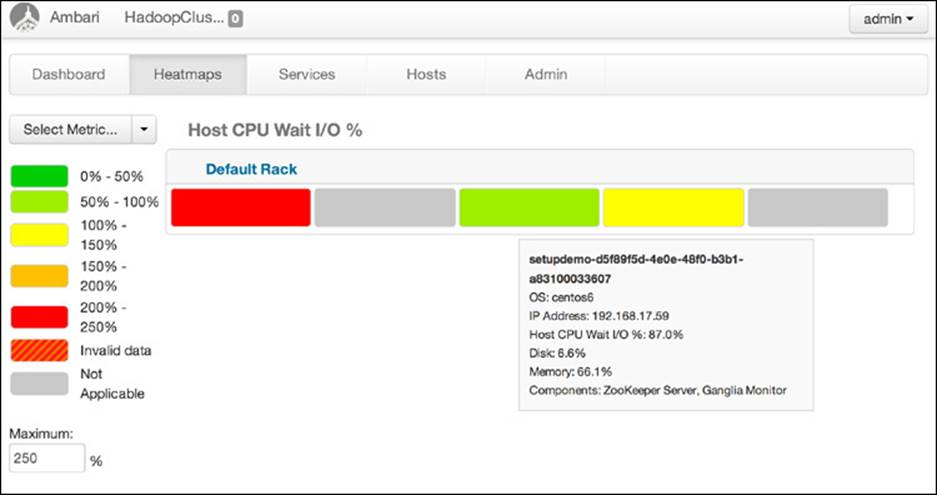
\includegraphics[scale=0.6]{media/chap9/ambari-heatmap.jpg}
    \caption{Ambari heatmap
    \label{fig:ambari-heatmap}}
\end{figure}

At every tested gram (i.e.~1, 2 and 3) the word ``heat map'' is a strong
predictor of type 4 bugs. The heat map feature is a complex feature as
it heavily relies on the underlying instrumentation of Hadoop and the
consumption of many log format too, for example, extracts the remaining
free space on a disk or the current load on a CPU.

Another word that is a strong predictor of type 4 bug is ``nagio''.
Nagio is a log monitoring server belonging to the Apache constellation.
It is used as an optional add-on for Ambari and, as for the heat map, is
very susceptible to log format change and API breakage.

Versions of the ``nagio'' and ``heatmap'' keywords include: ``heatmap
displai'', ``ambari heatmap'', ``fix nagio'', ``nagio test'', ``ambari
heatmap displai'', ``fix nagio test''.

\subsubsection{Cassandra}\label{cassandra}

Cassandra is a database with high scalability and high availability
without compromising performance. While extracting the unique word
combinations from the report of Cassandra, one word which is a strong
predictor of type 4 bug is ``snapshot''.

As described in the documentation, in Cassandra terms, \emph{a snapshot
first flushes all in-memory writes to disk, then makes a hard link of
the SSTable files for each keyspace. You must have enough free disk
space on the node to accommodate making snapshots of your data files. A
single snapshot requires little disk space. However, snapshots can cause
your disk usage to grow more quickly over time because a snapshot
prevents old obsolete data files from being deleted. After the snapshot
is complete, you can move the backup files to another location if
needed, or you can leave them in place.}

The definition gives the reader an insight into how complex this feature
used regarding integration with the host system and how coupled it is to
the Cassandra, data model.

Other versions of the ``snapshot'' keyword include ``snapshot
sequenti'', ``make snapshot'', ``snapshot sequenti repair'', ``make
snapshot sequenti''.

\subsubsection{Flume}\label{flume}

Flume is a distributed, reliable, and available service for efficiently
collecting, aggregating, and moving large amounts of log data.

One word which is a good predictor of type 4 in flume is ``upgrad'' and
the 2-grams (upgrad flume) and the 3-grams (``upgrad flume to'')
versions. Once again for the Apache dataset, a change in the software
that induce a change in the underlying data model or data store, which
is often the case when you upgrade flume to a new version, is a good
indicator of the report complexity and the impact of said report on the
sourcecode in terms of number of locations fixed.

On the reports manually analysed, Flume's developers and users have a
hard time upgrading to new versions in a sense that logs and dashboard
get corrupted or disappear post-upgrade. Significant efforts are then
made to prevent such losses in the subsequent version.

\subsubsection{HBase}\label{hbase}

HBase is a Hadoop database, a distributed, scalable, big data store
provided by Apache. The best predictor of type 4 bug in HBase is
``bloom'' as in ``bloom filters''. Bloom filters are a probabilistic
data structure that is used to test whether an element is a member of a
set {[}27{]}. Such a feature is hard to implement and hard to test
because of its probabilistic nature. Much feature commits (i.e.~commit
intended to add a feature) and fix commits (i.e.~commit intended to fix
a bug) belonging to the HBase source code are related to the bloom
filters. Given the nature of the feature, it is not surprising to find
the word ``bloom'' and its 2-, 3-grams counterparts (``on Bloom'',
``Bloom filter'', ``on Bloom filter'') as a good predictor of type 4
bug.

\subsubsection{Hive}\label{hive}

Hive is a data warehouse software facilitates reading, writing, and
managing large datasets residing in distributed storage using SQL. Hive
is different from its Apache counterpart as the words that are the best
predictors of type 4 bugs do not translate into a particular feature of
the product but are directly the name of the incriminated part of the
system: thrift. Thrift is a software framework, for scalable
cross-language services development, combines a software stack with a
code generation engine to build services that work efficiently and
seamlessly between C++, Java, Python, PHP, Ruby, Erlang, Perl, Haskell,
C\#, Cocoa, JavaScript, Node.js, Smalltalk, OCaml and Delphi and other
languages. While Thrift is supposed to solve many compatibility issues
when building clients for a product such as Hive, it is the cause of
many major problems in Hive. The top predictors for type 4 bugs in Hive
are ``thrifthttpcliservic'' and ``thriftbinarycliservic''.

As Hive, and its client, are built on top of Thrift it makes sense that
issues propagating from Thrift induce major refactoring and fixed across
the whole Hive source code.

\subsubsection{Cnd}\label{cnd}

The CND projects is a part of the Netbeans IDE and provide support for
C/C++. The top two predictors of type 4 bugs are (1) parallelism and (2)
observability of c/c++ code. In each gram, we can find reference to the
parallel code being problematic while developed and executed via the
Netbeans IDE: ``parallel comput'', ``parallel'', ``parallel comput
advis''. The other word, related to the observability of c/c++ code
inside the Netbeans IDE is ``Gizmo''. ``Gizmo'' is the codename for the
C/C++ Observability Tool built on top of D-Light Toolkit. We can find
occurrences of ``Gizmo'' in each gram: ``gizmo'' and ``gizmo monitor''
for example.

Once again, a complex cross-concern feature with a high impact on the
end-user (i.e., the ability to code, execute and debug parallel code
inside Netbeans) is the cause of most of the type 4 bugs and mention of
said feature in the report is a bug predictor of types of the bug.

\subsubsection{Editor}\label{editor}

The Editor component of Netbeans is the component which is handling all
the textual edition, regardless of the programming language, in
Netbeans. For this component, the type 4 bugs are most likely related to
the ``trailing white spaces'' and ``spellcheck'' features.

While these features do not, at first sight, be as complex as, for
example, parallelism debugging, they have been the cause of the majority
of type 4 bugs. Upon manual inspection of the related
code\footnote{https://netbeans.org/projects/editor/} in the Editor
component of Netbeans the complexity of these feature becomes evident.
Indeed, theses features behave differently for almost each type of
text-file and textboxes inside Netbeans. For example, the end-user
expects the spellchecking feature of the IDE to kick in while typing a
comment inside a code file but not on the code itself. A similar example
can be described for the identification and removing of trailing white
spaces where users wish the trailing white spaces to be deleted in c/c++
code but not, for example, while typing HTML or a commit message.

Each new language supported or add-on supported by the Netbeans IDE and
leveraging the features of the Editor component is susceptible to be the
cause of a major refactoring to have a coherent behaviour regarding
``trailing white spaces'' and ``spell checking''.

\subsubsection{Java}\label{java}

The Java component of Netbeans is responsible for the Java support of
Netbeans in the same fashion as CND is responsible for c/c++ support.
For this particular component, the set of features that are a good
predictor of type 4 are the ones related to the Java autocompletion and
navigation optimisation. The autocompletion has to be able to provide
suggestions in a near-instantaneous manner if it is to be useful to the
developer. To provide near-instantaneous suggestion on modest machines
and despite the depth of the Java API, Netbeans developers opted of a
statistical autocompletion. The autocompletion \emph{remembers} which of
its suggestions you used before and only provide the ones you are the
most likely to want to be based on your previous usage. Also, each
suggestion is companioned with a percentage which describes the number
of time you pick a given a suggestion over the other. One can envision a
such a system can be tricky to implement on new API being added in the
Java language at each upgrade. Indeed, when a new API comes to light
following a Java upgrade on the developer's machine, then, the
autocompletion has to make these new API appears in the autocompletion
despite their 0\% chosen rate. The 0\% being linked to the fact that
this suggestion was not available thus far and not to the fact that the
developer never picked it. When the new suggestion, related to the new
API, has been ignored a given number of time, then, it can be safely
removed from the list of suggestions.

Implementation of optimisations related to autocompletion and
navigations are the root causes of many type 4 bugs, and we can find
them in the gram extracted words that are good predictor: ``implement
optim'', ``move otim'', ``optim import implement'', ``call hierarchy
implement''.

\subsubsection{JavaEE}\label{javaee}

The JavaEE component of Netbeans is responsible for the support of the
JavaEE in Netbeans. This module is different from the CND and JAVA
module in a sense that it uses and expands many functionalities from the
JAVA component. For the JavaEE component, the best predictor of type 4
bugs is the hibernate and webscoket features which can be found in many
gram forms: ``hibern revers'', ``websocket endpoint'', ``hibern'',
``websocket'', ``implement hibern revers'', ``hibern revers engin''.

Hibernate is an ORM that enables developers to write applications whose
data outlives the application process more easily. As an
Object/Relational Mapping (ORM) framework, Hibernate is concerned with
data persistence as it applies to relational databases (via JDBC).

The shortcoming of Netbeans leading to most of the type 4 bugs is
related to the annotation based persistence of Hibernate where
developers can annotate their class attributes with the name of the
column they wish the value of the attribute to be persisted. While the
annotation mechanism is supported by Java, it is not possible
\emph{compile} annotation and makes sure that their statically sound.
Consequently, much tooling around annotation has to be developed and
maintained accordingly to new databases updates. Such tooling, for
example, is responsible for querying the database model to make sure
that the annotated columns exists and can store the attribute data
type-wise.

\subsubsection{Platform}\label{platform}

The last netbeans component we analyzed is the one named Platform.
\emph{The NetBeans Platform is a generic framework for Swing
applications. It provides the ``plumbing'' that, before, every developer
had to write themselves---saving state, connecting actions to menu
items, toolbar items and keyboard shortcuts; window management, and so
on.} (https://netbeans.org/features/platform/)

The best predictor of type 4 bug in the platform component is the
``filesystem'' word which refers to the ability of any application built
atop of Platform to use the filesystem for saves and such.

What we can conclude for this second research question is that the best
predictor of type 4 bugs is the mention of a cross-concern, complex,
widely used feature in the targeted system. Reports mentioning said
feature are likely to create a type 4 structure with many bugs being
fixed in the same set of files. One noteworthy observation is that the
2- and 3-grams extraction do not add much to the precision about the
1-gram extraction as seen the first research question. Upon the manual
analysis required for this research question, we can deduct why. Indeed,
the problematic features of a given system are identified with a single
word (i.e.~hibernate, filesystem, spellcheck, \ldots{}). While the 2-
and 3-grams classifiers do not provide an additional performance in the
classification process, they still become handy when trying to target
which part of the feature a good predictor of type 4 (``implement
optim'', ``gizmo monitor'', ``heatmap displai'', \ldots{}).

\section{Threats to Validity}\label{threats-to-validity-5}

The selection of target systems is one of the common threats to validity
for approaches that perform qualitative and quantitative analyses.

While is it possible the selected programs share common properties that
we are not aware of and therefore, invalidate our results, this is
highly unlikely. Indeed, our dataset is composed of 388 open source
systems.

In addition, we see a threat to validity that stems from the fact that
we only used open-source systems. The results may not be generalizable
to industrial systems. We intend to undertake these studies in future
work.

\section{Chapter Summary}\label{chapter-summary-5}

In this chapter, we proposed a taxonomy of bugs and performed an
empirical study on two large open source datasets: the Netbeans IDE and
the Apache Software Foundation's projects. Our study aimed to analyse:
(1) the proportion of each type of bugs; (2) the complexity of each type
in terms of severity, reopening and duplication; and (3) the required
time to fix a bug depending on its type. The key findings are that Type
4 account for 61\% of the bugs and have a bigger impact on software
maintenance tasks than the other three types.

In the next chapter, we start a discussion covering several topics
ranging from challenges sourrounding the adoption of tools to our advice
for university-industry research collaboration.

\chapter{Conclusion and Future Work}\label{conclusion-and-future-work}

In this chapter, we present the conclusion of this thesis and future
work that remain to be done.

Software maintenance activities such as debugging and feature
enhancement are known to be challenging and costly {[}157{]}. Studies
have shown that the cost of software maintenance can reach up to 70\% of
the overall cost of the software development life cycle {[}69{]}. Much
of this is attributable to several factors including the increase in
software complexity, the lack of traceability between the various
artifacts of the software development process, the lack of proper
documentation, and the unavailability of the original developers of the
systems.

In this thesis, we presented three approaches that perform software
maintenance at commit-time (PRECINCT, BIANCA and, CLEVER). We also
presented JCHARMING that can reproduce on field crash when commit-time
approaches did not catch the defect before its release. Finally, we also
propose a taxonomy of bugs that could be used by researchers to
categorize the research in many areas related to software maintenance.

\section{Summary of the Findings}\label{summary-of-the-findings}

\begin{itemize}
\item
  We created BUMPER, an aggregated, searchable bug-fix repository that
  contains 1,930 projects, 732,406 resolved/fixed, 1,645,252 changesets
  from Eclipse, Gnome, Netbeans and the Apache Software foundation.
\item
  We proposed PRECINCT, an incremental, online clone-detection approach
  that operates at commit-time. It was able to achieve an average 97.7\%
  precision and 100\% recall while requiring a fraction of the time
  thanks to its incremental approach.
\item
  We presented BIANCA, that detects risky commits and proposes potential
  fixes using clone-detection and dependency clustering. It was able to
  detect risky-commit with an average of 90.75\% precision and 37.15\%
  recall at commit-time. In addition, 78\% of the proposed fixes were
  automatically classified as qualitative using a similarity threshold
  with the actual fix.
\item
  Out of the 15,316 commits BIANCA classified as \emph{risky}, only
  1,320 (8.6\%) were because they were matching a defect-commit inside
  the same project. This supports the idea that within the same project,
  developers are not likely to introduce the same defect twice. Over
  similar projects, however, similar bugs are introduced.
\item
  We manually reviewed 250 fixes proposed by BIANCA. We were able to
  identify the statements from the proposed fixes that can be reused to
  create fixes similar to the ones that developers had proposed in 84\%
  of the cases.
\item
  While the recall of BIANCA 37.15\%, it is important to note that we do
  not claim that of issues in open-source systems are caused by project
  dependencies.
\item
  We built upon BIANCA with CLEVER that combines clone- and metric-based
  detection of risky commit and proposes potential fixes. It
  significantly reduced to scalability concerns of BIANCA while
  obtaining an average of 79.10\% precision and a 65.61\% recall.
\item
  66\% of the fixes proposed by CLEVER were accepted by software
  developer within Ubisoft.
\item
  We introduced JCHARMING, an automatic bug reproduction technique that
  combines crash traces and directed model checking. When applied to
  thirty bugs from ten open source systems, JCHARMING was able to
  successfully reproduce 80\% of the bugs. The average time to reproduce
  a bug was 19 minutes, which is quite reasonable, given the complexity
  of reproducing bugs that cause field crashes.
\item
  Finally, we proposed a taxonomy of bugs and performed an empirical.
  The key findings are that Type 4 account for 61\% of the bugs and have
  a bigger impact on software maintenance tasks than the other three
  types.
\end{itemize}

\section{Closing Remarks}\label{closing-remarks}

In this thesis, we proposed many approaches to help software developers
build high quality software systems. We chose to focus on techniques
that operate at commit-time. By doing so, this thesis' contributions
adhere to the broader concept of just-in-time software quality
improvement methods that promote the integration of software maintenance
and quality assurance tasks with day-to-day development {[}91, 190,
205{]}. Today's software systems are becoming ultra large, composed of
many components that interact with each other in a complex way. It is
often challenging for software developers to apply existing methods for
improving software quality such as clone detection, refactoring after
the system in its entirety has been built. This is because the mental
models and thought processes that led to these changes or design
decisions are long gone and forgotten. Just-in-time software improvement
techniques encourage an agile and lean process in which improvements are
made as soon as changes happen in the system, while the decisions
motivating the changes are still fresh in the mind of practitioners.
Agility and lean thinking are not new concepts. They date back to the
seventies where Toyota, the car manufacturer, proposed just-in-time
manufacturing techniques to produce high quality products that meet
customers' needs {[}179{]}.

Just-in-time manufacturing relies on several management philosophies and
tools: continuous improvement (product-oriented layout of plants,
division of systems, simplicity), elimination of waste (overproduction,
waiting time, inventory waste, transportation, product defects),
Hausukipingu (clean workspaces), Kabans (pulling the right number of
items from the right shelves at just the right time), Jidoka (autonomous
machines with judgment capabilities) and Andons (signal problems for
corrective action).\footnote{We kept the Japanese version of most of the
  words as they are used without translation in the literature.}

One of the cornerstones of the just-in-time manufacturing philosophy of
the seventies and the agile manifesto of the 2000's is continuous
improvement {[}59{]}. Other notions cross the gap between just-in-time
manufacturing and just-in-time software improvement. For example,
integrated development environments (IDEs) are Jidokas in a sense that
they auto-complete us and auto-correct us based on past behavior and,
unit tests, bug report management systems and quality assurance (QA)
bots are Andons.

PRECINCT, BIANCA, and CLEVER are designed to support just-in-time
software quality improvement and maintenance techniques by continuously
checking developer's code before ending up integrated into a larger
software system.

We believe that commit-time software maintenance is the appropriate time
to perform just-in-time software maintenance as commits mark the end of
a task or sub-task that is ready to be versioned.

JCHARMING adds value by proposing a mechanism for reproducing and fixing
the remaining defects. We hope that software engineering researchers and
practitioners find this work useful either as a starting point for
exciting new research or for building software products that are of good
quality.

\section{Future Work}\label{future-work}

\subsection{Current Limitations}\label{current-limitations}

We should acknowledge that the most notable shortcoming of this thesis
is the fact that we did not incorporate developers' opinions enough in
our studies. Indeed, we only gathered developers opinions' in two
separate occasions (BUMPER, Chapter 4 and CLEVER, Chapter 7). While
their opinions were positives, we should continue to ask practitioners
for their feedbacks on our work.

Another limitation of our work is that most of the approaches (BUMPER,
BIANCA and, CLEVER) will most likely be ineffective if applied to a
single-system. Indeed, these approaches rely on the large amount of data
acquired from multiple software ecosystems.

This leads to the scalability issues of our work. The model required to
operate BIANCA took nearly three months using 48 Amazon Virtual Private
Servers running in parallel to built and tested. While CLEVER addresses
some of the scalability issues with its two-step classifier, the search
of a potential solution is still computationally expansive.

\subsection{Other Possible Opportunities for Future
Research}\label{other-possible-opportunities-for-future-research}

To build on this work, we need to conduct experiment with additional (and
larger) systems with the dual aim of fine-tuning the approach, and
assessing the scalability of our approach when applied to even larger
systems could be conducted. Also, we want to improve PRECINCT to
support Type 4 clones, which will be a significant advantage over other
clone detectors. In addition, conducting user studies with developers to
assess the effectiveness of PRECINCT compared to remote and
local clone detection techniques.

Conducting user studies with developers in order to gather their
feedback on BIANCA and CLEVER would be beneficial. The feedback obtained
could help fine-tune the approaches. Also, examining the relationship
between project cluster measures (such as betweenness) and the
performance of BIANCA. Finally, another improvement to BIANCA would be
to support Type 4 clones.

For BIANCA, building a feedback loop between the users and the clusters
of known buggy commits and their fixes. If a fix is never used by the
end-users, then we could remove it from the clusters and improve our
accuracy.

For JCHARMING's, more experiments with more (and complex) bugs with the
dual aim to (a) improve and fine tune the approach, and (b) assess the
scalability of our approach when applied to even larger (and
proprietary) systems. Finally, comparing JCHARMING to STAR {[}31{]},
which is the closest approach to ours by running both methods on the
same set of systems and bugs, could yield interesting results. This
comparative study can provide insights into the differences in the use
of symbolic analysis as it is in STAR and directed model checking, the
core mechanism of JCHARMING.

\chapter{Appendices}\label{appendices}

\section{Lists of the top-level open-source
projects}\label{lists-of-the-top-level-open-source-projects}

Lists all the top-level open-source projects we analysed for our work.

\subsection{Parsers}\label{parsers}

\begin{itemize}
\tightlist
\item
  Mime4j: Apache James Mime4J provides a parser, MimeStreamParser, for
  e-mail message streams in plain rfc822 and MIME format
\item
  Xerces: XML parsers for c++, java and perl
\item
  Xalan:XSLT processor for transforming XML documents into HTML, text,
  or other XML document types.
\item
  FOP:Print formatter driven by XSL formatting objects (XSL-FO) and an
  output independent formatter.
\item
  Droids: intelligent standalone robot framework that allows to create
  and extend existing droids (robots).
\item
  Betwit: XML introspection mechanism for mapping beans to XML
\end{itemize}

\subsection{Databases}\label{databases}

\begin{itemize}
\tightlist
\item
  Drill: Schema-free SQL Query Engine for Hadoop, NoSQL and Cloud
  Storage
\item
  Tez: Frameword for complex directed-acyclic-graph of tasks for
  processing data.built atop Apache Hadoop YARN.
\item
  HBase: Apache HBase is the Hadoop database, a distributed, scalable,
  big data store.
\item
  Falcon: Falcon is a feed processing and feed management system aimed
  at making it easier for end consumers to onboard their feed processing
  and feed management on hadoop clusters.
\item
  Cassandra: Database with high scalability and high availability
  without compromising performance
\item
  Hive: Data warehouse software facilitates reading, writing, and
  managing large datasets residing in distributed storage using SQL
\item
  Sqoop: Tool designed for efficiently transferring bulk data between
  Apache Hadoop and structured datastores such as relational databases.
\item
  Accumulo: Sorted, distributed key/value store is a robust, scalable,
  high performance data storage and retrieval system.
\item
  Lucene: Full-featured text search engine library written entirely in
  Java. It is a technology suitable for nearly any application that
  requires full-text search, especially cross-platform.
\item
  CouchDB: Store your data with JSON documents. Access your documents
  and query your indexes with your web browser, via HTTP.
\item
  Phoenix: OLTP and operational analytics in Hadoop for low latency
  applications
\item
  OpenJPA: Java persistence project that can be used as a stand-alone
  POJO persistence layer or integrated into any Java EE
\item
  Gora: Provides an in-memory data model and persistence for big data
\item
  Optiq: framework that allows efficient translation of queries
  involving heterogeneous and federated data.
\item
  HCatalog: Table and storage management layer for Hadoop that enables
  users with different data processing tools
\item
  DdlUtils: Component for working with Database Definition (DDL) files
\item
  Derby: Relational database implemented entirely in Java
\item
  DBCP: Supports interaction with a relational database
\item
  JDO: Object persistence technology
\end{itemize}

\subsection{Web and Services}\label{web-and-services}

\begin{itemize}
\tightlist
\item
  Wicket: Server-side Java web framework
\item
  Service Mix: The components project holds a set of JBI (ava Business
  Integration) components that can be installed in both the ServiceMix 3
  and ServiceMix 4 containers.
\item
  Shindig: Apache Shindig is an OpenSocial container and helps you to
  start hosting OpenSocial apps quickly by providing the code to render
  gadgets, proxy requests, and handle REST and RPC requests.
\item
  Felix: Implement the OSGi Framework and Service platform and other
  interesting OSGi-related technologies under the Apache license.
\item
  Trinidad: JSF framework including a large, enterprise quality
  component library.
\item
  Axis: Web Services / SOAP / WSDL engine.
\item
  Synapse: Lightweight and high-performance Enterprise Service Bus
\item
  Giraph: Iterative graph processing system built for high scalability.
\item
  Tapestry: A component-oriented framework for creating highly scalable
  web applications in Java.
\item
  JSPWiki: WikiWiki engine, feature-rich and built around standard JEE
  components (Java, servlets, JSP).
\item
  TomEE: Java EE 6 Web Profile certified application server extends
  Apache Tomcat.
\item
  Knox: REST API Gateway for interacting with Apache Hadoop clusters.
\item
  Flex: Framework for building expressive web and mobile applications
\item
  Lucy: Search engine library provides full-text search for dynamic
  programming languages
\item
  Camel: Define routing and mediation rules in a variety of
  domain-specific languages, including a Java-based Fluent API, Spring
  or Blueprint XML Configuration files, and a Scala DSL.
\item
  Pivot: Builds installable Internet applications (IIAs)
\item
  Celix: Implementation of the OSGi specification adapted to C
\item
  Traffic Server: Fast, scalable and extensible HTTP/1.1 compliant
  caching proxy server.
\item
  Apache Net: Implements the client side of many basic Internet
  protocols. The purpose of the library is to provide fundamental
  protocol access, not higher-level abstractions.
\item
  Sling: Innovative web framework
\item
  Axis: Implementation of the SOAP (``Simple Object Access Protocol'')
  submission to W3C.
\item
  Shale: Web application framework, fundamentally based on JavaServer
  Faces.
\item
  Rave: web and social mashup engine that aggregates and serves web
  widgets.
\item
  Tuscany: Simplifies the task of developing SOA solutions by providing
  a comprehensive infrastructure for SOA development and management that
  is based on Service Component Architecture (SCA) standard.
\item
  Pluto: Implementation of the Java Portlet Specification.
\item
  ODE: Executes business processes written following the WS-BPEL
  standard
\item
  Muse: Java-based implementation of the WS-ResourceFramework (WSRF),
  WS-BaseNotification (WSN), and WS-DistributedManagement (WSDM)
  specifications.
\item
  WS-Commons: Web Services Commons Projects
\item
  Geronimo: Server runtime that integrates the best open source projects
  to create Java/OSGi
\item
  River: Network architecture for the construction of distributed
  systems in the form of modular co-operating services
\item
  Commons FileUpload: Makes it easy to add robust, high-performance,
  file upload capability to your servlets and web applications.
\item
  Beehive: Java Application Framework that was designed to simplify the
  development of Java EE based applications.
\item
  Aries: Java components enabling an enterprise OSGi application
  programming model.
\item
  Empire Db: Relational database abstraction layer and data persistence
  component
\item
  Commons Daemon: Java based daemons or services
\item
  Click: JEE web application framework
\item
  Stanbol: Provides a set of reusable components for semantic content
  management.
\item
  CXF: Open-Source Services Framework
\item
  Sandesha2: Axis2 module that implements the WS-ReliableMessaging
  specification published by IBM, Microsoft, BEA and TIBCO
\item
  Neethi: Framework for the programmers to use WS Policy
\item
  Rampart: Provides implementations of the WS-Sec* specifications for
  Apache Axis2.
\item
  AWF: web server
\item
  Nutch: Web crawler
\item
  HttpAsyncClient: Designed for extension while providing robust support
  for the base HTTP protocol
\item
  Portals Bridges: Portlet development using common web frameworks like
  Struts, JSF, PHP, Perl, Velocity and Scripts such as Groovy, JRuby,
  Jython, BeanShell or Rhino JavaScript.
\item
  Stonehenge: set of example applications for Service Oriented
  Architecture that spans languages and platforms and demonstrates best
  practices and interoperability.
\end{itemize}

\subsection{Cloud and Big data}\label{cloud-and-big-data}

\begin{itemize}
\tightlist
\item
  Whirr: Set of libraries for running cloud services
\item
  Ambari: Aimed at making Hadoop management simpler by developing
  software for provisioning, managing, and monitoring Apache Hadoop
  clusters.
\item
  Karaf: Karaf provides dual polymorphic container and application
  bootstrapping paradigms to the Enterprise.
\item
  Hadoop: Software for reliable, scalable, distributed computing.
\item
  Hama: framework for Big Data analytics which uses the Bulk Synchronous
  Parallel (BSP) computing model.
\item
  Twill: Abstraction over Apache Hadoop YARN that reduces the complexity
  of developing distributed applications
\item
  Hadoop MapReduce and Framework for easily writing applications which
  process vast amounts of data (multi-terabyte data-sets) in-parallel on
  large clusters (thousands of nodes) of commodity hardware in a
  reliable, fault-tolerant manner.
\item
  Tajo: Big data relational and distributed data warehouse system for
  Apache Hadoop
\item
  Sentry: System for enforcing fine grained role based authorization to
  data and metadata stored on a Hadoop cluster.
\item
  Oozie: Workflow scheduler system to manage Apache Hadoop jobs.
\item
  Solr: Provides distributed indexing, replication and load-balanced
  querying, automated failover and recovery, centralized configuration
\item
  Airavata: Software framework that enables you to compose, manage,
  execute, and monitor large scale applications
\item
  JClouds: Multi-cloud toolkit for the Java platform that gives you the
  freedom to create applications that are portable across clouds while
  giving you full control to use cloud-specific features.
\item
  Impala: Native analytic database for Apache Hadoop.
\item
  Libcloud: Python library for interacting with many of the popular
  cloud service providers using a unified API.
\item
  Slider: deploy existing distributed applications on an Apache Hadoop
  YARN cluster
\item
  MRUNIT: Java library that helps developers unit test Apache Hadoop map
  reduce jobs.
\item
  Stratos: Framework that helps run Apache Tomcat, PHP, and MySQL
  applications and can be extended to support many more environments on
  all major cloud infrastructures
\item
  Mesos: Abstracts CPU, memory, storage, and other compute resources
  away from machines
\item
  Helix: A cluster management framework for partitioned and replicated
  distributed resources
\item
  Argus: Centralized approach to security policy definition and
  coordinated enforcement
\item
  DeltaCloud: API that abstracts differences between clouds
\item
  MRQL: Query processing and optimization system for large-scale,
  distributed data analysis, built on top of Apache Hadoop, Hama, Spark,
  and Flink.
\item
  Provisionr: create and manage pools of virtual machines on multiple
  clouds
\item
  Curator: A ZooKeeper Keeper.
\item
  ZooKeeper: Open-source server which enables highly reliable
  distributed coordination
\item
  Bigtop: Infrastructure Engineers and Data Scientists looking for
  comprehensive packaging, testing, and configuration of the leading
  open source big data components.
\item
  Yarn: split up the functionalities of resource management and job
  scheduling/monitoring into separate daemons.
\end{itemize}

\subsection{Messaging and Logging}\label{messaging-and-logging}

\begin{itemize}
\tightlist
\item
  Activemq: Messaging queue
\item
  Qpid: Messaging queue
\item
  log4cxx: Logging framework for C++
\item
  log4j: Logging framework for Java
\item
  log4net: Logging framework for .Net
\item
  Flume: Distributed, reliable, and available service for efficiently
  collecting, aggregating, and moving large amounts of log data.
\item
  Samza: The project aims to provide a near-realtime, asynchronous
  computational framework for stream processing.
\item
  Pig: Analyzing large data sets that consists of a high-level language
  for expressing data analysis programs.
\item
  Chukwa: Data collection system for monitoring large distributed
  systems
\item
  BookKeeper: Replicated log service which can be used to build
  replicated state machines.
\item
  Apollo: Faster, more reliable, easier to maintain messaging broker
  built from the foundations of the original ActiveMQ.
\item
  S4: Processes continuous unbounded streams of data.
\end{itemize}

\subsection{Graphics}\label{graphics}

\begin{itemize}
\tightlist
\item
  Commons Imaging: Pure-Java Image Library
\item
  PDFBox: Java tool for working with PDF documents.
\item
  Batik: Java-based toolkit for applications or applets that want to use
  images in the Scalable Vector Graphics (SVG)
\item
  XML Graphics Commons: consists of several reusable components used by
  Apache Batik and Apache FOP
\item
  UIMA: UIMA frameworks, tools, and annotators, facilitating the
  analysis of unstructured content such as text, audio and video.
\end{itemize}

\subsection{Dependency Management and build
systems}\label{dependency-management-and-build-systems}

\begin{itemize}
\tightlist
\item
  Tentacles: Downloads all the archives from a staging repo, unpack them
  and create a little report of what is there.
\item
  Ivy: Transitive dependency manager
\item
  Rat: Release audit tool, focused on licenses.
\item
  Ant: drive processes described in build files as targets and extension
  points dependent upon each other
\item
  EasyAnt: Improved integration in existing build systems
\item
  IvyIDE: Eclipse plugin which integrates Apache Ivy's dependency
  management into Eclipse
\item
  NPanday: Maven for .NET
\item
  Maven: software project management and comprehension tool
\end{itemize}

\subsection{Networking}\label{networking}

\begin{itemize}
\tightlist
\item
  Mina:100\% pure java library to support the SSH protocols on both the
  client and server side.
\item
  James:Delivers a rich set of open source modules and libraries,
  written in Java, related to Internet mail communication which build
  into an advanced enterprise mail server.
\item
  Hupa:Rich IMAP-based Webmail application written in GWT (Google Web
  Toolkit).
\item
  Etch:cross-platform, language and transport-independent framework for
  building and consuming network services
\item
  Commons IO: Library of utilities to assist with developing IO
  functionality.
\end{itemize}

\subsection{File systems and
repository}\label{file-systems-and-repository}

\begin{itemize}
\tightlist
\item
  Tika: detects and extracts metadata and text from over a thousand
  different file types
\item
  OODT: Apache Object Oriented Data Technology (OODT) is a smart way to
  integrate and archive your processes, your data, and its metadata.
\item
  Commons Virtual File System: Provides a single API for accessing
  various different file systems.
\item
  Jackrabbit Oak: Scalable and performant hierarchical content
  repository
\item
  Directory: Provides directory solutions entirely written in Java.
\item
  SANDBOX: Subversion repository for Commons committers to function as
  an open workspace for sharing and collaboration.
\end{itemize}

\subsection{Misc}\label{misc}

\begin{itemize}
\tightlist
\item
  Harmony: Modular Java runtime with class libraries and associated
  tools.
\item
  Mahout: Machine learning applications.
\item
  OpenCMIS: Apache Chemistry OpenCMIS is a collection of Java libraries,
  frameworks and tools around the CMIS specification.
\item
  Apache Commons: Apache project focused on all aspects of reusable Java
  components
\item
  Shiro: Java security framework
\item
  Cordova: Mobile apps with HTML, CSS \& JS
\item
  XMLBeans: Technology for accessing XML by binding it to Java types
\item
  State Chart XML: Provides a generic state-machine based execution
  environment based on Harel State Tables
\item
  excalibur: lightweight, embeddable Inversion of Control
\item
  Commons Transaction: Transactional Java programming
\item
  Velocity: collection of POJO
\item
  BCEL: analyze, create, and manipulate binary Java class files
\item
  Abdera: Functionally-complete, high-performance implementation of the
  IETF Atom Syndication Format
\item
  Commons Collections: Data structures that accelerate development of
  most significant Java applications.
\item
  Java Caching System: Distributed caching system written in Java
\item
  OGNL: Object-Graph Navigation Language; it is an expression language
  for getting and setting properties of Java objects, plus other extras
  such as list projection and selection and lambda expressions.
\item
  Anything To Triples: library that extracts structured data in RDF
  format from a variety of Web documents.
\item
  Axiom: provides an XML Infoset compliant object model implementation
  which supports on-demand building of the object tree
\item
  Graft: debugging and testing tool for programs written for Apache
  Giraph
\item
  Hivemind: Services and configuration microkernel
\item
  JXPath: defines a simple interpreter of an expression language called
  XPath
\end{itemize}

\section*{Bibliography}

\setlength{\parindent}{0pt}

\hypertarget{refs}{}
\hypertarget{ref-Alencar2014}{}
{[}1{]} Alencar, D., Abebe, S.L. and Mcintosh, S. 2014. An Empirical
Study of Delays in the Integration of Addressed Issues. \emph{Software
maintenance and evolution (iCSME)} (2014).

\hypertarget{ref-Antoniol2002}{}
{[}2{]} Antoniol, G., Canfora, G., Casazza, G., De Lucia, A. and Merlo,
E. 2002. Recovering traceability links between code and documentation.
\emph{IEEE Transactions on Software Engineering}. 28, 10 (Oct. 2002),
970--983.

\hypertarget{ref-Anvik2006}{}
{[}3{]} Anvik, J., Hiew, L. and Murphy, G.C. 2006. Who should fix this
bug? \emph{Proceeding of the 28th international conference on software
engineering - iCSE '06} (New York, New York, USA, May 2006), 361.

\hypertarget{ref-ApacheSoftwareFoundation}{}
{[}4{]} Apache Software Foundation Apache Ant.

\hypertarget{ref-ApacheSoftwareFoundation2014}{}
{[}5{]} Apache Software Foundation 2014. Apache PDFBox \textbar{} A Java
PDF Library.

\hypertarget{ref-ApacheSoftwareFoundation2000}{}
{[}6{]} Apache Software Foundation 2000. Apache Struts Project.

\hypertarget{ref-hadoop2011hadoop}{}
{[}7{]} Apache Software Fundation 2011. Hadoop.

\hypertarget{ref-mahout2012scalable}{}
{[}8{]} Apache Software Fundation 2012. Mahout: Scalable machine
learning and data mining.

\hypertarget{ref-Artzi2008}{}
{[}9{]} Artzi, S., Kim, S. and Ernst, M.D. 2008. Recrash: Making
software failures reproducible by preserving object states.
\emph{Proceedings of the 22nd european conference on object-oriented
programming} (2008), 542--565.

\hypertarget{ref-Avizienis2004}{}
{[}10{]} Avizienis, A., Laprie, J.-C., Randell, B. and Landwehr, C.
2004. Basic concepts and taxonomy of dependable and secure computing.
\emph{IEEE Transactions on Dependable and Secure Computing}. 1, 1 (Jan.
2004), 11--33.

\hypertarget{ref-Ayewah2007}{}
{[}11{]} Ayewah, N., Pugh, W., Morgenthaler, J.D., Penix, J. and Zhou,
Y. 2007. Evaluating static analysis defect warnings on production
software. \emph{Proceedings of the 7th aCM sIGPLAN-sIGSOFT workshop on
program analysis for software tools and engineering - pASTE '07} (New
York, New York, USA, Jun. 2007), 1--8.

\hypertarget{ref-Bachmann2010}{}
{[}12{]} Bachmann, A., Bird, C., Rahman, F., Devanbu, P. and Bernstein,
A. 2010. The missing links. \emph{Proceedings of the eighteenth aCM
sIGSOFT international symposium on foundations of software engineering -
fSE '10} (New York, New York, USA, Nov. 2010), 97.

\hypertarget{ref-Baier2008}{}
{[}13{]} Baier, C. and Katoen, J.-P. 2008. \emph{Principles of Model
Checking}. MIT press Cambridge.

\hypertarget{ref-Baker}{}
{[}14{]} Baker, B. 1995. On finding duplication and near-duplication in
large software systems. \emph{Proceedings of the 2nd working conference
on reverse engineering} (1995), 86--95.

\hypertarget{ref-Balazinska}{}
{[}15{]} Balazinska, M., Merlo, E., Dagenais, M., Lague, B. and
Kontogiannis, K. 1999. Partial redesign of Java software systems based
on clone analysis. \emph{Proceedings of the sixth working conference on
reverse engineering} (1999), 326--336.

\hypertarget{ref-Basili1996}{}
{[}16{]} Basili, V., Briand, L. and Melo, W. 1996. A validation of
object-oriented design metrics as quality indicators. \emph{IEEE
Transactions on Software Engineering}. 22, 10 (1996), 751--761.

\hypertarget{ref-Bavota2013}{}
{[}17{]} Bavota, G., Canfora, G., Penta, M.D., Oliveto, R. and
Panichella, S. 2013. The Evolution of Project Inter-dependencies in a
Software Ecosystem: The Case of Apache. \emph{2013 iEEE international
conference on software maintenance} (Sep. 2013), 280--289.

\hypertarget{ref-Baxter1998}{}
{[}18{]} Baxter, I.D., Yahin, A., Moura, L., Sant'Anna, M. and Bier, L.
1998. Clone Detection Using Abstract Syntax Trees. \emph{Proceedings of
the iEEE international conference on software maintenance.} (Mar. 1998),
368--377.

\hypertarget{ref-Beckwith2006}{}
{[}19{]} Beckwith, L., Kissinger, C., Burnett, M., Wiedenbeck, S.,
Lawrance, J., Blackwell, A. and Cook, C. 2006. Tinkering and gender in
end-user programmers' debugging. \emph{Proceedings of the sIGCHI
conference on human factors in computing systems} (2006), 231--240.

\hypertarget{ref-Bell2013}{}
{[}20{]} Bell, J., Sarda, N. and Kaiser, G. 2013. Chronicler:
Lightweight recording to reproduce field failures. \emph{2013 35th
international conference on software engineering (iCSE)} (May 2013),
362--371.

\hypertarget{ref-Bellon2007}{}
{[}21{]} Bellon, S., Koschke, R., Antoniol, G., Krinke, J. and Merlo, E.
2007. Comparison and Evaluation of Clone Detection Tools. \emph{IEEE
Transactions on Software Engineering}. 33, 9 (Sep. 2007), 577--591.

\hypertarget{ref-Bettenburg2008}{}
{[}22{]} Bettenburg, N., Just, S., Schröter, A., Weiss, C., Premraj, R.
and Zimmermann, T. 2008. What makes a good bug report? \emph{Proceedings
of the 16th aCM sIGSOFT international symposium on foundations of
software engineering} (New York, New York, USA, 2008), 308.

\hypertarget{ref-Bettenburg2008a}{}
{[}23{]} Bettenburg, N., Premraj, R. and Zimmermann, T. 2008. Duplicate
bug reports considered harmful \ldots{} really? \emph{2008 iEEE
international conference on software maintenance} (2008), 337--345.

\hypertarget{ref-Bhattacharya2011}{}
{[}24{]} Bhattacharya, P. and Neamtiu, I. 2011. Bug-fix time prediction
models: can we do better? \emph{Proceeding of the international
conference on mining software repositories} (New York, New York, USA,
May 2011), 207--210.

\hypertarget{ref-Bortis2013}{}
{[}25{]} Bortis, G. and Hoek, A. van der 2013. PorchLight: A tag-based
approach to bug triaging. \emph{2013 35th international conference on
software engineering (iCSE)} (May 2013), 342--351.

\hypertarget{ref-Briand1999a}{}
{[}26{]} Briand, L., Daly, J. and Wust, J. 1999. A unified framework for
coupling measurement in object-oriented systems. \emph{IEEE Transactions
on Software Engineering}. 25, 1 (1999), 91--121.

\hypertarget{ref-Broder2004}{}
{[}27{]} Broder, A. and Mitzenmacher, M. 2004. Network Applications of
Bloom Filters: A Survey. \emph{Internet Mathematics}. 1, 4 (Jan. 2004),
485--509.

\hypertarget{ref-Bugzilla2008}{}
{[}28{]} Bugzilla 2008. Life Cycle of a Bug.

\hypertarget{ref-Burg2013}{}
{[}29{]} Burg, B., Bailey, R., Ko, A.J. and Ernst, M.D. 2013.
Interactive record/replay for web application debugging.
\emph{Proceedings of the 26th annual aCM symposium on user interface
software and technology} (New York, New York, USA, Oct. 2013), 473--484.

\hypertarget{ref-Burnstein2006}{}
{[}30{]} Burnstein, I. 2006. \emph{Practical Software Testing: A
Process-Oriented Approach}. Springer Science \& Business Media.

\hypertarget{ref-Chen2013a}{}
{[}31{]} Chen, N. 2013. \emph{Star: stack trace based automatic crash
reproduction}. Honk Kong University of Science; Technology.

\hypertarget{ref-Chen2013}{}
{[}32{]} Chen, N. 2013. \emph{Star: stack trace based automatic crash
reproduction}. The Hong Kong University of Science; Technology.

\hypertarget{ref-Chen2014}{}
{[}33{]} Chen, T.-h., Nagappan, M., Shihab, E. and Hassan, A.E. 2014. An
Empirical Study of Dormant Bugs Categories and Subject Descriptors.
\emph{Proceedings of the international conference on mining software
repository} (2014), 82--91.

\hypertarget{ref-Chidamber1994}{}
{[}34{]} Chidamber, S. and Kemerer, C. 1994. A metrics suite for object
oriented design. \emph{IEEE Transactions on Software Engineering}. 20, 6
(Jun. 1994), 476--493.

\hypertarget{ref-ChrisVignola2014}{}
{[}35{]} Chris Vignola 2014. The Java Community Process(SM) Program -
JSRs: Java Specification Requests - detail JSR\# 352.

\hypertarget{ref-Clause2007}{}
{[}36{]} Clause, J. and Orso, A. 2007. A Technique for Enabling and
Supporting Debugging of Field Failures. \emph{Proceedings of the 29th
international conference on software engineering} (2007), 261--270.

\hypertarget{ref-CollabNet}{}
{[}37{]} CollabNet Tigris.org: Open Source Software Engineering.

\hypertarget{ref-Cordy2006a}{}
{[}38{]} Cordy, J.R. 2006. Source transformation, analysis and
generation in TXL. \emph{Proceedings of the symposium on partial
evaluation and semantics-based program manipulation} (New York, New
York, USA, Jan. 2006), 1--11.

\hypertarget{ref-Cordy2011}{}
{[}39{]} Cordy, J.R. and Roy, C.K. 2011. The NiCad Clone Detector.
\emph{Proceedings of the international conference on program
comprehension} (Jun. 2011), 219--220.

\hypertarget{ref-Czerwonka2013}{}
{[}40{]} Czerwonka, J., Nagappan, N., Schulte, W. and Murphy, B. 2013.
CODEMINE: Building a Software Development Data Analytics Platform at
Microsoft. \emph{IEEE Software}. 30, 4 (Jul. 2013), 64--71.

\hypertarget{ref-DAmbros2010}{}
{[}41{]} D'Ambros, M., Lanza, M. and Robbes, R. 2010. An extensive
comparison of bug prediction approaches. \emph{2010 7th iEEE working
conference on mining software repositories (mSR 2010)} (May 2010),
31--41.

\hypertarget{ref-Dallmeier}{}
{[}42{]} Dallmeier, V., Zeller, A. and Meyer, B. 2009. Generating Fixes
from Object Behavior Anomalies. \emph{Proceedings of the international
conference on automated software engineering} (2009), 550--554.

\hypertarget{ref-Dangel2000}{}
{[}43{]} Dangel, A. 2000. PMD.

\hypertarget{ref-de2001program}{}
{[}44{]} De Lucia, A. 2001. Program slicing: Methods and applications.
\emph{International working conference on source code analysis and
manipulation} (2001), 144.

\hypertarget{ref-de2008z3}{}
{[}45{]} De Moura, L. and Bjørner, N. 2008. Z3: An efficient SMT solver.
\emph{Tools and algorithms for the construction and analysis of
systems}. Springer. 337--340.

\hypertarget{ref-Dean}{}
{[}46{]} Dean, T.R., Cordy, J.R., Malton, A.J. and Schneider, K.A. 2003.
Agile Parsing in TXL. \emph{Proceedings of the international conference
on automated software engineering} (2003), 311--336.

\hypertarget{ref-demange2013}{}
{[}47{]} Demange, A., Moha, N. and Tremblay, G. 2013. Detection of SOA
Patterns. \emph{Proceedings of the international conference on
service-oriented computing} (2013), 114--130.

\hypertarget{ref-StephaneDucasse}{}
{[}48{]} Ducasse, S., Rieger, M. and Demeyer, S. 1999. A Language
Independent Approach for Detecting Duplicated Code. \emph{Proceedings of
the international conference on software maintenance} (1999), 109--118.

\hypertarget{ref-Dutertre2006}{}
{[}49{]} Dutertre, B. and Moura, L.D. 2006. The yices smt solver.
\emph{Tool paper at http://yices.csl.sri.com/tool-paper.pdf}. 2, 2
(2006).

\hypertarget{ref-Dyer2013}{}
{[}50{]} Dyer, R., Nguyen, H.A., Rajan, H. and Nguyen, T.N. 2013. Boa: a
language and infrastructure for analyzing ultra-large-scale software
repositories. \emph{Proceedings of the international conference on
software engineering} (May 2013), 422--431.

\hypertarget{ref-Edelkamp2004}{}
{[}51{]} Edelkamp, S., Leue, S. and Lluch-Lafuente, A. 2004. Directed
explicit-state model checking in the validation of communication
protocols. \emph{International Journal on Software Tools for Technology
Transfer (STTT)}. 5, 2-3 (Mar. 2004), 247--267.

\hypertarget{ref-Edelkamp2009}{}
{[}52{]} Edelkamp, S., Schuppan, V., Bosnacki, D., Wijs, A.,
FehnkerAnsgar and Aljazzar, H. 2009. \emph{Survey on directed model
checking}. Springer.

\hypertarget{ref-ElEmam2001}{}
{[}53{]} El Emam, K., Melo, W. and Machado, J.C. 2001. The prediction of
faulty classes using object-oriented design metrics. \emph{Journal of
Systems and Software}. 56, 1 (Feb. 2001), 63--75.

\hypertarget{ref-Eldh2001}{}
{[}54{]} Eldh, S. 2001. \emph{On Test Design}. Mälardalen.

\hypertarget{ref-Eyolfson2011}{}
{[}55{]} Eyolfson, J., Tan, L. and Lam, P. 2011. Do time of day and
developer experience affect commit bugginess. \emph{Proceeding of the
8th working conference on mining software repositories - mSR '11} (New
York, New York, USA, May 2011), 153.

\hypertarget{ref-Fischer}{}
{[}56{]} Fischer, M., Pinzger, M. and Gall, H. Populating a Release
History Database from version control and bug tracking systems.
\emph{International conference on software maintenance, 2003. iCSM 2003.
proceedings.} 23--32.

\hypertarget{ref-Fleiss1973}{}
{[}57{]} Fleiss, J.L. and Cohen, J. 1973. The Equivalence of Weighted
Kappa and the Intraclass Correlation Coefficient as Measures of
Reliability. \emph{Educational and Psychological Measurement}. 33, 3
(Oct. 1973), 613--619.

\hypertarget{ref-Foss2015}{}
{[}58{]} Foss, S.L. and Murphy, G.C. 2015. Do developers respond to code
stability warnings? \emph{Proceedings of the 25th annual international
conference on computer science and software engineering} (Nov. 2015),
162--170.

\hypertarget{ref-fowler2001agile}{}
{[}59{]} Fowler, M. and Highsmith, J. 2001. The agile manifesto.
\emph{Software Development}. 9, 8 (2001), 28--35.

\hypertarget{ref-Gabel2008}{}
{[}60{]} Gabel, M., Jiang, L. and Su, Z. 2008. Scalable detection of
semantic clones. \emph{Proceedings of the 13th international conference
on software engineering} (New York, New York, USA, 2008), 321--330.

\hypertarget{ref-Girvan2002}{}
{[}61{]} Girvan, M. and Newman, M.E.J. 2002. Community structure in
social and biological networks. \emph{Proceedings of the National
Academy of Sciences}. 99, 12 (Jun. 2002), 7821--7826.

\hypertarget{ref-Gode2009}{}
{[}62{]} Göde, N. and Koschke, R. 2009. Incremental Clone Detection.
\emph{Proceedings of the 13th european conference on software
maintenance and reengineering} (2009), 219--228.

\hypertarget{ref-Graphwalker2016}{}
{[}63{]} Graphwalker 2016. GraphWalker for testers.
\emph{Http://graphwalker.github.io/} (2016).

\hypertarget{ref-Gyimothy2005}{}
{[}64{]} Gyimothy, T., Ferenc, R. and Siket, I. 2005. Empirical
validation of object-oriented metrics on open source software for fault
prediction. \emph{IEEE Transactions on Software Engineering}. 31, 10
(Oct. 2005), 897--910.

\hypertarget{ref-Hamill2014}{}
{[}65{]} Hamill, M. and Goseva-Popstojanova, K. 2014. Exploring fault
types, detection activities, and failure severity in an evolving
safety-critical software system. \emph{Software Quality Journal}. 23, 2
(Apr. 2014), 229--265.

\hypertarget{ref-Hassan2005}{}
{[}66{]} Hassan, A. and Holt, R. 2005. The top ten list: dynamic fault
prediction. \emph{Proceedings of the international conference on
software maintenance} (2005), 263--272.

\hypertarget{ref-Hassan2009}{}
{[}67{]} Hassan, A.E. 2009. Predicting faults using the complexity of
code changes. \emph{Proceedings of the international conference on
software engineering} (May 2009), 78--88.

\hypertarget{ref-Havelund2015}{}
{[}68{]} Havelund, K., Holzmann, G. and Joshi, R. eds. 2015. \emph{NASA
Formal Methods}. Springer International Publishing.

\hypertarget{ref-HealthSocial2002}{}
{[}69{]} Health, Social and Research, E. 2002. \emph{The Economic
Impacts of Inadequate Infrastructure for Software Testing}.

\hypertarget{ref-Herbold2011}{}
{[}70{]} Herbold, S., Grabowski, J., Waack, S. and Bünting, U. 2011.
Improved Bug Reporting and Reproduction through Non-intrusive GUI Usage
Monitoring and Automated Replaying. \emph{2011 iEEE fourth international
conference on software testing, verification and validation workshops}
(Mar. 2011), 232--241.

\hypertarget{ref-Herraiz2008}{}
{[}71{]} Herraiz, I., German, D.M., Gonzalez-Barahona, J.M. and Robles,
G. 2008. Towards a simplification of the bug report form in eclipse.
\emph{Proceedings of the 2008 international workshop on mining software
repositories - mSR '08} (New York, New York, USA, May 2008), 145.

\hypertarget{ref-Higo2011}{}
{[}72{]} Higo, Y., Yasushi, U., Nishino, M. and Kusumoto, S. 2011.
Incremental Code Clone Detection: A PDG-based Approach.
\emph{Proceedings of the 18th working conference on reverse engineering}
(Oct. 2011), 3--12.

\hypertarget{ref-Hindle2008}{}
{[}73{]} Hindle, A., German, D.M. and Holt, R. 2008. What do large
commits tell us?: a taxonomical study of large commits.
\emph{Proceedings of the international workshop on mining software
repositories} (New York, New York, USA, 2008), 99--108.

\hypertarget{ref-holzmann1997model}{}
{[}74{]} Holzmann, G.J. 1997. The model checker SPIN. \emph{IEEE
Transactions on Software Engineering}. 23, 5 (1997), 279--295.

\hypertarget{ref-Hovemeyer2007}{}
{[}75{]} Hovemeyer, D. 2007. FindBugs.

\hypertarget{ref-Hummel2010}{}
{[}76{]} Hummel, B., Juergens, E., Heinemann, L. and Conradt, M. 2010.
Index-based code clone detection: incremental, distributed, scalable.
\emph{Proceedings of the iEEE international conference on software
maintenance} (Sep. 2010), 1--9.

\hypertarget{ref-Hunt1977}{}
{[}77{]} Hunt, J.W. and Szymanski, T.G. 1977. A fast algorithm for
computing longest common subsequences. \emph{Communications of the ACM}.
20, 5 (May 1977), 350--353.

\hypertarget{ref-IBM2006}{}
{[}78{]} IBM 2006. T. J. Watson Libraries for Analysis (WALA).

\hypertarget{ref-Jalbert2008}{}
{[}79{]} Jalbert, N. and Weimer, W. 2008. Automated duplicate detection
for bug tracking systems. \emph{2008 iEEE international conference on
dependable systems and networks with fTCS and dCC (dSN)} (2008), 52--61.

\hypertarget{ref-Jaygarl}{}
{[}80{]} Jaygarl, H., Kim, S., Xie, T. and Chang, C.K. 2010. OCAT:
Object Capture based Automated Testing. \emph{Proceedings of the 19th
international symposium on software testing and analysis} (2010),
159--170.

\hypertarget{ref-Jeong2009}{}
{[}81{]} Jeong, G., Kim, S. and Zimmermann, T. 2009. Improving bug
triage with bug tossing graphs. \emph{Proceedings of the the 7th joint
meeting of the european software engineering conference and the aCM
sIGSOFT symposium on the foundations of software engineering} (New York,
New York, USA, Aug. 2009), 111.

\hypertarget{ref-Jiang2007}{}
{[}82{]} Jiang, L., Misherghi, G., Su, Z. and Glondu, S. 2007. DECKARD:
Scalable and Accurate Tree-Based Detection of Code Clones.
\emph{Proceedings of the 29th international conference on software
engineering} (May 2007), 96--105.

\hypertarget{ref-Jin2012}{}
{[}83{]} Jin, W. and Orso, A. 2012. BugRedux: Reproducing field failures
for in-house debugging. \emph{Proceedings of the 34th international
conference on software engineering, iEEE} (Jun. 2012), 474--484.

\hypertarget{ref-Jin2013}{}
{[}84{]} Jin, W. and Orso, A. 2013. F3: fault localization for field
failures. \emph{Proceedings of the 2013 international symposium on
software testing and analysis} (New York, New York, USA, 2013),
213--223.

\hypertarget{ref-Johnson2013}{}
{[}85{]} Johnson, B., Song, Y., Murphy-Hill, E. and Bowdidge, R. 2013.
Why don't software developers use static analysis tools to find bugs?
\emph{Proceedings of the international conference on software
engineering} (May 2013), 672--681.

\hypertarget{ref-Johnson1993}{}
{[}86{]} Johnson, J.H. 1993. Identifying redundancy in source code using
fingerprints. \emph{Proceedings of the conference of the centre for
advanced studies on collaborative research} (Oct. 1993), 171--183.

\hypertarget{ref-Johnson1994}{}
{[}87{]} Johnson, J.H. 1994. Visualizing textual redundancy in legacy
source. \emph{Proceedings of the conference of the centre for advanced
studies on collaborative research} (Oct. 1994), 32.

\hypertarget{ref-JoshuaOMadadhain}{}
{[}88{]} Joshua O'Madadhain, Danyel Fisher, Scott White, Padhraic Smyth,
Y.-b.B. 2005. Analysis and Visualization of Network Data using JUNG.
\emph{Journal of Statistical Software}. 10, 2 (2005), 1--35.

\hypertarget{ref-Juergens2009}{}
{[}89{]} Juergens, E., Deissenboeck, F., Hummel, B. and Wagner, S. 2009.
Do code clones matter? \emph{Proceedings of the iEEE 31st international
conference on software engineering} (May 2009), 485--495.

\hypertarget{ref-Jung2009}{}
{[}90{]} Jung, Y., Oh, H. and Yi, K. 2009. Identifying static analysis
techniques for finding non-fix hunks in fix revisions. \emph{Proceeding
of the aCM first international workshop on data-intensive software
management and mining - dSMM '09} (New York, New York, USA, Nov. 2009),
13.

\hypertarget{ref-Kamei2013}{}
{[}91{]} Kamei, Y., Shihab, E., Adams, B., Hassan, A.E., Mockus, A.,
Sinha, A. and Ubayashi, N. 2013. A large-scale empirical study of
just-in-time quality assurance. \emph{IEEE Transactions on Software
Engineering}. 39, 6 (Jun. 2013), 757--773.

\hypertarget{ref-Kamiya2002}{}
{[}92{]} Kamiya, T., Kusumoto, S. and Inoue, K. 2002. CCFinder: a
multilinguistic token-based code clone detection system for large scale
source code. \emph{IEEE Transactions on Software Engineering}. 28, 7
(Jul. 2002), 654--670.

\hypertarget{ref-Kapser}{}
{[}93{]} Kapser, C. and Godfrey, M. 2004. Aiding comprehension of
cloning through categorization. \emph{Proceedings. 7th international
workshop on principles of software evolution, 2004.} (2004), 85--94.

\hypertarget{ref-Kapser2006}{}
{[}94{]} Kapser, C. and Godfrey, M. 2006. Cloning Considered Harmful
Considered Harmful. \emph{Proceedings of the 13th working conference on
reverse engineering} (Oct. 2006), 19--28.

\hypertarget{ref-CoryKapser}{}
{[}95{]} Kapser, C. and Godfrey, M.W. 2003. Toward a Taxonomy of Clones
in Source Code: A Case Study. \emph{International workshop on evolution
of large scale industrial software architectures} (2003), 67--78.

\hypertarget{ref-Kim2013}{}
{[}96{]} Kim, D., Nam, J., Song, J. and Kim, S. 2013. Automatic patch
generation learned from human-written patches. \emph{Proceedings of the
international conference on software engineering} (May 2013), 802--811.

\hypertarget{ref-Kim2011c}{}
{[}97{]} Kim, D., Wang, X., Member, S., Kim, S., Zeller, A., Cheung,
S.C., Member, S. and Park, S. 2011. Which Crashes Should I Fix First?:
Predicting Top Crashes at an Early Stage to Prioritize Debugging
Efforts. \emph{TRANSACTIONS ON SOFTWARE ENGINEERING}. 37, 3 (2011),
430--447.

\hypertarget{ref-Kim2005}{}
{[}98{]} Kim, M., Sazawal, V. and Notkin, D. 2005. An empirical study of
code clone genealogies. \emph{ACM SIGSOFT Software Engineering Notes}.
30, 5 (Sep. 2005), 187--196.

\hypertarget{ref-Kim2006}{}
{[}99{]} Kim, S., Zimmermann, T., Pan, K. and Jr. Whitehead, E. 2006.
Automatic Identification of Bug-Introducing Changes. \emph{Proceedings
of the international conference on automated software engineering}
(2006), 81--90.

\hypertarget{ref-Kim2006c}{}
{[}100{]} Kim, S., Zimmermann, T., Pan, K. and Jr. Whitehead, E. 2006.
Automatic Identification of Bug-Introducing Changes. \emph{Proceedings
of the international conference on automated software engineering}
(2006), 81--90.

\hypertarget{ref-Kim2007a}{}
{[}101{]} Kim, S., Zimmermann, T., Whitehead Jr., E.J. and Zeller, A.
2007. Predicting Faults from Cached History. \emph{Proceedings of the
international conference on software engineering} (May 2007), 489--498.

\hypertarget{ref-Kim2007}{}
{[}102{]} Kim, S., Zimmermann, T., Whitehead Jr., E.J. and Zeller, A.
2007. Predicting Faults from Cached History. \emph{Proceedings of the
international conference on software engineering} (May 2007), 489--498.

\hypertarget{ref-Ko2006d}{}
{[}103{]} Ko, A., Myers, B., Coblenz, M. and Aung, H. 2006. An
Exploratory Study of How Developers Seek, Relate, and Collect Relevant
Information during Software Maintenance Tasks. \emph{IEEE Transactions
on Software Engineering}. 32, 12 (Dec. 2006), 971--987.

\hypertarget{ref-Kontogiannis}{}
{[}104{]} Kontogiannis, K. 1997. Evaluation experiments on the detection
of programming patterns using software metrics. \emph{Proceedings of the
fourth working conference on reverse engineering} (1997), 44--54.

\hypertarget{ref-Koponen2006}{}
{[}105{]} Koponen, T. 2006. Life cycle of defects in open source
software projects. \emph{Open source systems} (2006), 195--200.

\hypertarget{ref-Kpodjedo2010}{}
{[}106{]} Kpodjedo, S., Ricca, F., Galinier, P., Guéhéneuc, Y.-G. and
Antoniol, G. 2010. Design evolution metrics for defect prediction in
object oriented systems. \emph{Empirical Software Engineering}. 16, 1
(Dec. 2010), 141--175.

\hypertarget{ref-Krinke2001}{}
{[}107{]} Krinke, J. 2001. Identifying Similar Code with Program
Dependence Graphs. \emph{Proceedings of the eighth iEEE working
conference on reverse engineering} (Oct. 2001), 301--309.

\hypertarget{ref-Kripke1963}{}
{[}108{]} Kripke, S.A. 1963. Semantical Considerations on Modal Logic.
\emph{Acta Philosophica Fennica}. 16, 1963 (1963), 83--94.

\hypertarget{ref-kropf1999introduction}{}
{[}109{]} Kropf, T. 1999. \emph{Introduction to formal hardware
verification}. Springer.

\hypertarget{ref-Lamkanfi2010}{}
{[}110{]} Lamkanfi, A., Demeyer, S., Giger, E. and Goethals, B. 2010.
Predicting the severity of a reported bug. \emph{2010 7th iEEE working
conference on mining software repositories (mSR 2010)} (May 2010),
1--10.

\hypertarget{ref-Landis1977}{}
{[}111{]} Landis, J.R. and Koch, G.G. 1977. The Measurement of Observer
Agreement for Categorical Data. \emph{Biometrics}. 33, 1 (Mar. 1977),
159.

\hypertarget{ref-LaToza2006}{}
{[}112{]} Latoza, T.D., Venolia, G. and DeLine, R. 2006. Maintaining
mental models: a study of developer work habits. \emph{Proceeding of the
28th international conference on software engineering - iCSE '06} (New
York, New York, USA, 2006), 492--501.

\hypertarget{ref-Layman2007}{}
{[}113{]} Layman, L., Williams, L. and Amant, R.S. 2007. Toward Reducing
Fault Fix Time: Understanding Developer Behavior for the Design of
Automated Fault Detection Tools. \emph{Proceedings of the first
international symposium on empirical software engineering and
measurement (eSEM 2007)} (Sep. 2007), 176--185.

\hypertarget{ref-le2012systematic}{}
{[}114{]} Le Goues, C., Dewey-Vogt, M., Forrest, S. and Weimer, W. 2012.
A systematic study of automated program repair: Fixing 55 out of 105
bugs for \$8 each. \emph{Proceedings of the international conference on
software engineering} (2012), 3--13.

\hypertarget{ref-le2015should}{}
{[}115{]} Le, X.-B.D., Le, T.-D.B. and Lo, D. 2015. Should fixing these
failures be delegated to automated program repair? \emph{Proceedings of
the international symposium on software reliability engineering} (2015),
427--437.

\hypertarget{ref-Lee2011a}{}
{[}116{]} Lee, T., Nam, J., Han, D., Kim, S. and In, H.P. 2011. Micro
interaction metrics for defect prediction. \emph{Proceedings of the
european conference on foundations of software engineering} (New York,
New York, USA, 2011), 311--231.

\hypertarget{ref-Lewis2013}{}
{[}117{]} Lewis, C., Lin, Z., Sadowski, C., Zhu, X., Ou, R. and
Whitehead Jr., E.J. 2013. Does bug prediction support human developers?
Findings from a google case study. \emph{Proceedings of the
international conference on software engineering} (May 2013), 372--381.

\hypertarget{ref-Li2006}{}
{[}118{]} Li, Z., Lu, S., Myagmar, S. and Zhou, Y. 2006. CP-Miner:
finding copy-paste and related bugs in large-scale software code.
\emph{IEEE Transactions on Software Engineering}. 32, 3 (Mar. 2006),
176--192.

\hypertarget{ref-Lo2013}{}
{[}119{]} Lo, D. 2013. A Comparative Study of Supervised Learning
Algorithms for Re-opened Bug Prediction. \emph{Proceedings of the
european conference on software maintenance and reengineering} (Mar.
2013), 331--334.

\hypertarget{ref-Maiga2015}{}
{[}120{]} Maiga, A., Hamou-Lhadj, A., Nayrolles, M., Koochekian Sabor,
K. and Larsson, A. 2015. An empirical study on the handling of crash
reports in a large software company: An experience report. \emph{2015
iEEE 31st international conference on software maintenance and
evolution, iCSME 2015 - proceedings} (2015), 342--351.

\hypertarget{ref-Manber1994}{}
{[}121{]} Manber, U. 1994. Finding similar files in a large file system.
\emph{Proceedings of the usenix winter} (Jan. 1994), 1--10.

\hypertarget{ref-Manevich2004}{}
{[}122{]} Manevich, R., Sridharan, M. and Adams, S. 2004. PSE:
explaining program failures via postmortem static analysis. \emph{ACM
sIGSOFT software engineering notes} (Nov. 2004), 63.

\hypertarget{ref-Marcus}{}
{[}123{]} Marcus, A. and Maletic, J. 2001. Identification of high-level
concept clones in source code. \emph{Proceedings international
conference on automated software engineering} (2001), 107--114.

\hypertarget{ref-MartinFowler2009}{}
{[}124{]} Martin Fowler 2009. FeatureBranch.

\hypertarget{ref-mcmillan1993symbolic}{}
{[}125{]} McMillan, K.L. 1993. \emph{Symbolic model checking}. Springer.

\hypertarget{ref-Menzies2008}{}
{[}126{]} Menzies, T. and Marcus, A. 2008. Automated severity assessment
of software defect reports. \emph{2008 iEEE international conference on
software maintenance} (Sep. 2008), 346--355.

\hypertarget{ref-menzies2007problems}{}
{[}127{]} Menzies, T., Dekhtyar, A., Distefano, J. and Greenwald, J.
2007. Problems with Precision: A Response to`` Comments on'Data Mining
Static Code Attributes to Learn Defect Predictors'''. \emph{IEEE
Transactions on Software Engineering}. 33, 9 (2007), 637.

\hypertarget{ref-Moha}{}
{[}128{]} Moha, N., Palma, F., Nayrolles, M., Joyen-Conseil, B.,
Guéhéneuc, Y.-G., Baudry, B. and Jézéquel, J.-M. 2012. Specification and
Detection of SOA Antipatterns. \emph{Procedings of the International
Conference on Service Oriented Computing}. (2012), 1--16.

\hypertarget{ref-Nagappan2005}{}
{[}129{]} Nagappan, N. and Ball, T. 2005. Static analysis tools as early
indicators of pre-release defect density. \emph{Proceedings of the
international conference on software engineering} (New York, New York,
USA, May 2005), 580--586.

\hypertarget{ref-Nagappan}{}
{[}130{]} Nagappan, N. and Ball, T. 2005. Use of relative code churn
measures to predict system defect density. \emph{Proceedings of the
international conference on software engineering} (2005), 284--292.

\hypertarget{ref-Nagappan2006}{}
{[}131{]} Nagappan, N., Ball, T. and Zeller, A. 2006. Mining metrics to
predict component failures. \emph{Proceeding of the international
conference on software engineering} (New York, New York, USA, May 2006),
452--461.

\hypertarget{ref-Nam2013}{}
{[}132{]} Nam, J., Pan, S.J. and Kim, S. 2013. Transfer defect learning.
\emph{Proceedings of the international conference on software
engineering} (May 2013), 382--391.

\hypertarget{ref-Narayanasamy2005}{}
{[}133{]} Narayanasamy, S., Pokam, G. and Calder, B. 2005. BugNet:
Continuously Recording Program Execution for Deterministic Replay
Debugging. \emph{Proceedings of the 32nd annual international symposium
on computer architecture} (May 2005), 284--295.

\hypertarget{ref-NASA2009}{}
{[}134{]} NASA 2009. Open Mission Control Technologies.

\hypertarget{ref-Nayrolles2018}{}
{[}135{]} Nayrolles, M. and Hamou-lhadj, A. 2018. CLEVER: Combining Code
Metrics with Clone Detection for Just-In-Time Fault Prevention and
Resolution in Large Industrial Projects. \emph{Mining software
repositories} (2018).

\hypertarget{ref-Nayrolles2016b}{}
{[}136{]} Nayrolles, M. and Hamou-Lhadj, W. 2016. BUMPER: A Tool to Cope
with Natural Language Search of Millions Bugs and Fixes.
\emph{International conference on software analysis, evolution, and
reengineering} (2016), 649--652.

\hypertarget{ref-Nayrolles2015}{}
{[}137{]} Nayrolles, M., Hamou-Lhadj, A., Sofiene, T. and Larsson, A.
2015. JCHARMING : A Bug Reproduction Approach Using Crash Traces and
Directed Model Checking. \emph{Proceedings of the 22nd international
conference on software analysis, evolution, and reengineering} (2015),
101--110.

\hypertarget{ref-Nayrolles2016d}{}
{[}138{]} Nayrolles, M., Hamou-Lhadj, A., Tahar, S. and Larsson, A.
2016. A bug reproduction approach based on directed model checking and
crash traces. \emph{Journal of Software: Evolution and Process}. (2016).

\hypertarget{ref-Nayrolles2015g}{}
{[}139{]} Nayrolles, M., Hamou-Lhadj, A., Tahar, S. and Larsson, A.
2015. JCHARMING: A bug reproduction approach using crash traces and
directed model checking. \emph{2015 iEEE 22nd international conference
on software analysis, evolution, and reengineering, sANER 2015 -
proceedings} (2015).

\hypertarget{ref-Nayrolles}{}
{[}140{]} Nayrolles, M., Maiga, A., Hamou-lhadj, A. and Larsson, A. A
Taxonomy of Bugs : An Empircial Study. 1--10.

\hypertarget{ref-Nayrolles2013a}{}
{[}141{]} Nayrolles, M., Moha, N. and Valtchev, P. 2013. Improving SOA
Antipatterns Detection in Service Based Systems by Mining Execution
Traces. \emph{Working conference on reverse engineering} (2013),
321--330.

\hypertarget{ref-Nessa2008}{}
{[}142{]} Nessa, S., Abedin, M., Wong, W.E., Khan, L. and Qi, Y. 2008.
Software Fault Localization Using N -gram Analysis. \emph{WASA} (2008),
548--559.

\hypertarget{ref-Newman2004}{}
{[}143{]} Newman, M.E.J. and Girvan, M. 2004. Finding and evaluating
community structure in networks. \emph{Physical Review E}. 69, 2 (Feb.
2004), 026113.

\hypertarget{ref-Nguyen2012}{}
{[}144{]} Nguyen, A.T., Nguyen, T.T., Nguyen, T.N., Lo, D. and Sun, C.
2012. Duplicate bug report detection with a combination of information
retrieval and topic modeling. \emph{Proceedings of the 27th iEEE/ACM
international conference on automated software engineering - aSE 2012}
(New York, New York, USA, 2012), 70.

\hypertarget{ref-Nguyen2012a}{}
{[}145{]} Nguyen, H.A., Nguyen, T.T., Pham, N.H., Al-Kofahi, J. and
Nguyen, T.N. 2012. Clone Management for Evolving Software. \emph{IEEE
Transactions on Software Engineering}. 38, 5 (Sep. 2012), 1008--1026.

\hypertarget{ref-Nguyen2009}{}
{[}146{]} Nguyen, T.T., Nguyen, H.A., Pham, N.H., Al-Kofahi, J.M. and
Nguyen, T.N. 2009. Clone-Aware Configuration Management.
\emph{Proceedings of the iEEE/ACM international conference on automated
software engineering} (Nov. 2009), 123--134.

\hypertarget{ref-Niko2012}{}
{[}147{]} Niko, S., Mircea, L. and Romain, R. 2012. On how often code is
cloned across repositories. \emph{Proceedings of the 34th international
conference on software engineering} (2012), 1289--1292.

\hypertarget{ref-OSullivan2009}{}
{[}148{]} O'Sullivan, B. and Bryan 2009. Making sense of
revision-control systems. \emph{Communications of the ACM}. 52, 9 (Sep.
2009), 56.

\hypertarget{ref-ObjectRefineryLimited2005}{}
{[}149{]} Object Refinery Limited 2005. JFreeChart.

\hypertarget{ref-Oracle2011}{}
{[}150{]} Oracle 2011. Throwable (Java Plateform SE6).

\hypertarget{ref-Ostrand2005}{}
{[}151{]} Ostrand, T., Weyuker, E. and Bell, R. 2005. Predicting the
location and number of faults in large software systems. \emph{IEEE
Transactions on Software Engineering}. 31, 4 (Apr. 2005), 340--355.

\hypertarget{ref-Palma2013}{}
{[}152{]} Palma, F. 2013. \emph{Detection of SOA Antipatterns}. Ecole
Polytechnique de Montreal.

\hypertarget{ref-Pan2008}{}
{[}153{]} Pan, K., Kim, S. and Whitehead, E.J. 2008. Toward an
understanding of bug fix patterns. \emph{Empirical Software
Engineering}. 14, 3 (Aug. 2008), 286--315.

\hypertarget{ref-Patenaude1999}{}
{[}154{]} Patenaude, J.-F., Merlo, E., Dagenais, M. and Lague, B. 1999.
Extending software quality assessment techniques to Java systems.
\emph{Proceedings seventh international workshop on program
comprehension} (1999), 49--56.

\hypertarget{ref-PerryDewayneE.1993}{}
{[}155{]} Perry, Dewayne E. and Stieg., C.S. 1993. Software faults in
evolving a large, real-time system: a case study. \emph{Software
engineering---ESEC} (1993), 48--67.

\hypertarget{ref-Pratt2001}{}
{[}156{]} Pratt, M.J. 2001. Introduction to ISO 10303---the STEP
Standard for Product Data Exchange. \emph{Journal of Computing and
Information Science in Engineering}. 1, 1 (Mar. 2001), 102.

\hypertarget{ref-Pressman2005}{}
{[}157{]} Pressman, R.S. 2005. \emph{Software Engineering: A
Practitioner's Approach}. Palgrave Macmillan.

\hypertarget{ref-Radatz1990}{}
{[}158{]} Radatz, J., Geraci, A. and Katki, F. 1990. IEEE standard
glossary of software engineering terminology. \emph{IEEE Std}.
610121990, 121990 (1990), 3.

\hypertarget{ref-rahman2013}{}
{[}159{]} Rahman, F. and Devanbu, P. 2013. How, and why, process metrics
are better. \emph{Proceedings of the international conference on
software engineering} (2013), 432--441.

\hypertarget{ref-Robertson2006}{}
{[}160{]} Robertson, T.J., Lawrance, J. and Burnett, M. 2006. Impact of
high-intensity negotiated-style interruptions on end-user debugging.
\emph{Journal of Visual Languages and Computing}. 17, 2 (2006),
187--202.

\hypertarget{ref-Robertson2004}{}
{[}161{]} Robertson, T.J., Prabhakararao, S., Burnett, M., Cook, C.,
Ruthruff, J.R., Beckwith, L. and Phalgune, A. 2004. Impact of
interruption style on end-user debugging. \emph{Proceedings of the
sIGCHI conference on human factors in computing systems} (2004),
287--294.

\hypertarget{ref-Roehm2015}{}
{[}162{]} Roehm, T., Nosovic, S. and Bruegge, B. 2015. Automated
extraction of failure reproduction steps from user interaction traces.
\emph{2015 iEEE 22nd international conference on software analysis,
evolution, and reengineering (sANER)} (Mar. 2015), 121--130.

\hypertarget{ref-Rosen2015}{}
{[}163{]} Rosen, C., Grawi, B. and Shihab, E. 2015. Commit guru:
analytics and risk prediction of software commits. \emph{Proceedings of
the joint meeting on foundations of software engineering} (New York, New
York, USA, Aug. 2015), 966--969.

\hypertarget{ref-Rossler2013}{}
{[}164{]} Rößler, J., Zeller, A., Fraser, G., Zamfir, C. and Candea, G.
2013. Reconstructing Core Dumps. \emph{Proceedings of the 6th
international conference on software testing, verification and
validation, ser. iCST} (2013).

\hypertarget{ref-Iss2009}{}
{[}165{]} Roy, C.K. 2009. \emph{Detection and Analysis of Near-Miss
Software Clones}. Queen's University.

\hypertarget{ref-Roy2008}{}
{[}166{]} Roy, C.K. and Cordy, J.R. 2008. An Empirical Study of Function
Clones in Open Source Software. \emph{Proceedings of the working
conference on reverse engineering} (Oct. 2008), 81--90.

\hypertarget{ref-Runeson2007}{}
{[}167{]} Runeson, P., Alexandersson, M. and Nyholm, O. 2007. Detection
of Duplicate Defect Reports Using Natural Language Processing.
\emph{29th international conference on software engineering} (May 2007),
499--510.

\hypertarget{ref-Saha2014}{}
{[}168{]} Saha, R.K., Khurshid, S. and Perry, D.E. 2014. An empirical
study of long lived bugs. \emph{2014 software evolution week - iEEE
conference on software maintenance, reengineering, and reverse
engineering (cSMR-wCRE)} (Feb. 2014), 144--153.

\hypertarget{ref-Saini2016}{}
{[}169{]} Saini, V., Sajnani, H., Kim, J. and Lopes, C. 2016.
SourcererCC and SourcererCC-I: : Tools to Detect Clones in Batch mode
and During Software Development. \emph{Proceedings of the 38th
international conference on software engineering} (New York, New York,
USA, 2016), 597--600.

\hypertarget{ref-Sajnani2016}{}
{[}170{]} Sajnani, H., Saini, V., Svajlenko, J., Roy, C.K. and Lopes,
C.V. 2016. SourcererCC: scaling code clone detection to big-code.
\emph{Proceedings of the 38th international conference on software
engineering} (New York, New York, USA, 2016), 1157--1168.

\hypertarget{ref-Seinturier2012}{}
{[}171{]} Seinturier, L., Merle, P., Rouvoy, R., Romero, D., Schiavoni,
V. and Stefani, J.-B. 2012. A component-based middleware platform for
reconfigurable service-oriented architectures. \emph{Software: Practice
and Experience}. 42, 5 (2012), 559--583.

\hypertarget{ref-Shihab2010}{}
{[}172{]} Shihab, E., Ihara, A., Kamei, Y., Ibrahim, W.M., Ohira, M.,
Adams, B., Hassan, A.E. and Matsumoto, K.-i. 2010. Predicting Re-opened
Bugs: A Case Study on the Eclipse Project. \emph{2010 17th working
conference on reverse engineering} (Oct. 2010), 249--258.

\hypertarget{ref-Shivaji2013}{}
{[}173{]} Shivaji, S., Member, S., Member, S., Akella, R. and Kim, S.
2013. Reducing Features to Improve Code Change-Based Bug Prediction.
\emph{IEEE Transactions on Software Engineering}. 39, 4 (2013),
552--569.

\hypertarget{ref-snyder2011activemq}{}
{[}174{]} Snyder, B., Bosanac, D. and Davies, R. 2011. \emph{ActiveMQ in
Action}. Manning Publications Co.

\hypertarget{ref-Steven2000}{}
{[}175{]} Steven, J., Chandra, P., Fleck, B. and Podgurski, A. 2000.
jRapture: A Capture/Replay Tool for Observation-Based Testing.
\emph{Proceedings of the international symposium on software testing and
analysis.} (2000), 158--167.

\hypertarget{ref-Subramanyam2003}{}
{[}176{]} Subramanyam, R. and Krishnan, M. 2003. Empirical analysis of
CK metrics for object-oriented design complexity: implications for
software defects. \emph{IEEE Transactions on Software Engineering}. 29,
4 (Apr. 2003), 297--310.

\hypertarget{ref-Sun2011}{}
{[}177{]} Sun, C., Lo, D., Khoo, S.-C. and Jiang, J. 2011. Towards more
accurate retrieval of duplicate bug reports. \emph{2011 26th IEEE/ACM
International Conference on Automated Software Engineering (ASE 2011)}.
(Nov. 2011), 253--262.

\hypertarget{ref-SunghunKim2008}{}
{[}178{]} Sunghun Kim, S., Whitehead, E. and Yi Zhang, Y. 2008.
Classifying Software Changes: Clean or Buggy? \emph{IEEE Transactions on
Software Engineering}. 34, 2 (Mar. 2008), 181--196.

\hypertarget{ref-suzaki1987new}{}
{[}179{]} Suzaki, K. 1987. \emph{New manufacturing challenge: Techniques
for continuous improvement}. Simon; Schuster.

\hypertarget{ref-Tairas2006a}{}
{[}180{]} Tairas, R., Gray, J. and Baxter, I. 2006. Visualization of
clone detection results. \emph{Proceedings of the 2006 oOPSLA workshop
on eclipse technology eXchange} (New York, New York, USA, 2006), 50--54.

\hypertarget{ref-Tamrawi2011a}{}
{[}181{]} Tamrawi, A., Nguyen, T.T., Al-Kofahi, J. and Nguyen, T.N.
2011. Fuzzy set-based automatic bug triaging. \emph{Proceeding of the
33rd international conference on software engineering - iCSE '11} (New
York, New York, USA, 2011), 884.

\hypertarget{ref-tao2014automatically}{}
{[}182{]} Tao, Y., Kim, J., Kim, S. and Xu, C. 2014. Automatically
generated patches as debugging aids: a human study. \emph{Proceedings of
the international symposium on foundations of software engineering}
(2014), 64--74.

\hypertarget{ref-TheApacheSoftwareFoundation2015}{}
{[}183{]} The Apache Software Foundation 2015. Apache BatchEE.
\emph{Http://batchee.incubator.apache.org/} (2015).

\hypertarget{ref-TheApacheSoftwareFoundation1999}{}
{[}184{]} The Apache Software Foundation 1999. Log4j 2 Guide - Apache
Log4j 2.

\hypertarget{ref-Tian2012}{}
{[}185{]} Tian, Y., Lo, D. and Sun, C. 2012. Information Retrieval Based
Nearest Neighbor Classification for Fine-Grained Bug Severity
Prediction. \emph{2012 19th working conference on reverse engineering}
(Oct. 2012), 215--224.

\hypertarget{ref-Tian2012a}{}
{[}186{]} Tian, Y., Sun, C. and Lo, D. 2012. Improved Duplicate Bug
Report Identification. \emph{2012 16th european conference on software
maintenance and reengineering} (Mar. 2012), 385--390.

\hypertarget{ref-TinKamHo}{}
{[}187{]} Tin Kam Ho 1995. Random decision forests. \emph{Proceedings of
the international conference on document analysis and recognition}
(1995), 278--282.

\hypertarget{ref-TinKamHo1998}{}
{[}188{]} Tin Kam Ho 1998. The random subspace method for constructing
decision forests. \emph{IEEE Transactions on Pattern Analysis and
Machine Intelligence}. 20, 8 (1998), 832--844.

\hypertarget{ref-Toomey2012}{}
{[}189{]} Toomey, W. 2012. Ctcompare: Code clone detection using hashed
token sequences. \emph{Proceedings of the 6th international workshop on
software clones} (Jun. 2012), 92--93.

\hypertarget{ref-Tourani2016}{}
{[}190{]} Tourani, P. and Adams, B. 2016. The Impact of Human
Discussions on Just-in-Time Quality Assurance: An Empirical Study on
OpenStack and Eclipse. \emph{23rd international conference on software
analysis, evolution, and reengineering} (Mar. 2016), 189--200.

\hypertarget{ref-Tufano2015}{}
{[}191{]} Tufano, M., Palomba, F., Bavota, G., Oliveto, R., Di Penta,
M., De Lucia, A. and Poshyvanyk, D. 2015. When and why your code starts
to smell bad. (May 2015), 403--414.

\hypertarget{ref-ValdiviaGarcia2014}{}
{[}192{]} Valdivia Garcia, H. and Shihab, E. 2014. Characterizing and
predicting blocking bugs in open source projects. \emph{Proceedings of
the 11th working conference on mining software repositories - mSR 2014}
(New York, New York, USA, May 2014), 72--81.

\hypertarget{ref-Visser2003}{}
{[}193{]} Visser, W., Havelund, K., Brat, G., Park, S. and Lerda, F.
2003. Model Checking Programs. \emph{Automated software engineering}
(2003), 203--232.

\hypertarget{ref-Visser2004}{}
{[}194{]} Visser, W., Pǎsǎreanu, C.S. and Khurshid, S. 2004. Test input
generation with java PathFinder. \emph{Proceedings of the 2004 ACM
SIGSOFT International Symposium on Software Testing and Analysis}.
(2004), 97.

\hypertarget{ref-Wahler}{}
{[}195{]} Wahler, V., Seipel, D., Wolff, J. and Fischer, G. 2004. Clone
detection in source code by frequent itemset techniques.
\emph{Proceedings of the fourth iEEE international workshop on source
code analysis and manipulation} (2004), 128--135.

\hypertarget{ref-Wang2011}{}
{[}196{]} Wang, X.(., Baik, E. and Devanbu, P.T. 2011. System
compatibility analysis of Eclipse and Netbeans based on bug data.
\emph{Proceeding of the 8th working conference on mining software
repositories - mSR '11} (New York, New York, USA, May 2011), 230.

\hypertarget{ref-Weiss2007}{}
{[}197{]} Weiss, C., Premraj, R., Zimmermann, T. and Zeller, A. 2007.
How Long Will It Take to Fix This Bug? \emph{Fourth international
workshop on mining software repositories (mSR'07:ICSE workshops 2007)}
(May 2007), 1--1.

\hypertarget{ref-Weiuxdf2007}{}
{[}198{]} Weiß, C., Zimmermann, T. and Zeller, A. 2007. How Long will it
Take to Fix This Bug ? \emph{Fourth international workshop on mining
software repositories (mSR'07)} (2007), 1.

\hypertarget{ref-Wellington2013}{}
{[}199{]} Wellington, B. 2013. Dnsjava.

\hypertarget{ref-Wettel2005}{}
{[}200{]} Wettel, R. and Marinescu, R. 2005. Archeology of code
duplication: recovering duplication chains from small duplication
fragments. \emph{Proceedings of the seventh international symposium on
symbolic and numeric algorithms for scientific computing} (2005),
63--71.

\hypertarget{ref-Whittaker2012}{}
{[}201{]} Whittaker, J.A., Arbon, J. and Carollo, J. 2012. \emph{How
Google Tests Software}. Addison-Wesley.

\hypertarget{ref-Wu2011}{}
{[}202{]} Wu, R., Zhang, H., Kim, S. and Cheung, S. 2011. Relink:
recovering links between bugs and changes. \emph{Proceedings of the
european conference on foundations of software engineering} (2011),
15--25.

\hypertarget{ref-Xuan2012}{}
{[}203{]} Xuan, J., Jiang, H., Ren, Z. and Zou, W. 2012. Developer
prioritization in bug repositories. \emph{2012 34th international
conference on software engineering (iCSE)} (Jun. 2012), 25--35.

\hypertarget{ref-yamanaka2012industrial}{}
{[}204{]} Yamanaka, Y., Choi, E., Yoshida, N., Inoue, K. and Sano, T.
2012. Industrial application of clone change management system.
\emph{Proceedings of the 6th international workshop on software clones}
(2012), 67--71.

\hypertarget{ref-Yang2015}{}
{[}205{]} Yang, X., Lo, D., Xia, X., Zhang, Y. and Sun, J. 2015. Deep
Learning for Just-in-Time Defect Prediction. \emph{2015 iEEE
international conference on software quality, reliability and security}
(Aug. 2015), 17--26.

\hypertarget{ref-Zamfir2010}{}
{[}206{]} Zamfir, C. and Candea, G. 2010. Execution Synthesis: A
Technique for Automated Software Debugging. \emph{Proceedings of the 5th
european conference on computer systems} (2010), 321--334.

\hypertarget{ref-Zeller1997}{}
{[}207{]} Zeller, A. 1997. \emph{Configuration management with version
sets: A unified software versioning model and its applications}.

\hypertarget{ref-Zeller2013a}{}
{[}208{]} Zeller, A. 2013. Where Should We Fix This Bug? A Two-Phase
Recommendation Model. \emph{IEEE Transactions on Software Engineering}.
39, 11 (Nov. 2013), 1597--1610.

\hypertarget{ref-Zeller2002}{}
{[}209{]} Zeller, A. and Hildebrandt, R. 2002. Simplifying and isolating
failure-inducing input. \emph{IEEE Transactions on Software
Engineering}. 28, 2 (2002), 183--200.

\hypertarget{ref-Zhang2012}{}
{[}210{]} Zhang, F., Khomh, F., Zou, Y. and Hassan, A.E. 2012. An
Empirical Study on Factors Impacting Bug Fixing Time. \emph{2012 19th
working conference on reverse engineering} (Oct. 2012), 225--234.

\hypertarget{ref-Zhang2013a}{}
{[}211{]} Zhang, G., Peng, X., Xing, Z., Shihai Jiang, Hai Wang and
Zhao, W. 2013. Towards contextual and on-demand code clone management by
continuous monitoring. \emph{28th iEEE/ACM international conference on
automated software engineering} (Nov. 2013), 497--507.

\hypertarget{ref-Zhang2013}{}
{[}212{]} Zhang, H., Gong, L. and Versteeg, S. 2013. Predicting
bug-fixing time: an empirical study of commercial software projects.
\emph{International conference on software engineering} (May 2013),
1042--1051.

\hypertarget{ref-Zhou2012}{}
{[}213{]} Zhou, J., Zhang, H. and Lo, D. 2012. Where should the bugs be
fixed? More accurate information retrieval-based bug localization based
on bug reports. \emph{Proceedings of the 34th international conference
on software engineering, iEEE} (Jun. 2012), 14--24.

\hypertarget{ref-Zibran2012}{}
{[}214{]} Zibran, M.F. and Roy, C.K. 2012. IDE-based real-time focused
search for near-miss clones. \emph{Proceedings of the 27th annual aCM
symposium on applied computing} (New York, New York, USA, 2012),
1235--1242.

\hypertarget{ref-Zibran2011}{}
{[}215{]} Zibran, M.F. and Roy, C.K. 2011. Towards flexible code clone
detection, management, and refactoring in IDE. \emph{Proceeding of the
5th international workshop on software clones} (New York, New York, USA,
2011), 75--76.

\hypertarget{ref-Zimmermann2008}{}
{[}216{]} Zimmermann, T. and Nagappan, N. 2008. Predicting defects using
network analysis on dependency graphs. \emph{Proceedings of the
international conference on software engineering} (New York, New York,
USA, May 2008), 531.

\hypertarget{ref-Zimmermann2012}{}
{[}217{]} Zimmermann, T., Nagappan, N., Guo, P.J. and Murphy, B. 2012.
Characterizing and predicting which bugs get reopened. \emph{Proceedings
of the 34th international conference on software engineering, iEEE}
(Jun. 2012), 1074--1083.

\hypertarget{ref-Zimmermann2007}{}
{[}218{]} Zimmermann, T., Premraj, R. and Zeller, A. 2007. Predicting
Defects for Eclipse. \emph{Proceedings of the international workshop on
predictor models in software engineering} (May 2007), 9.

\hypertarget{ref-Zuddas2014}{}
{[}219{]} Zuddas, D., Jin, W., Pastore, F., Mariani, L. and Orso, A.
2014. MIMIC: locating and understanding bugs by analyzing mimicked
executions. \emph{Proceedings of the 29th aCM/IEEE international
conference on automated software engineering} (New York, New York, USA,
Sep. 2014), 815--826.

\addcontentsline{toc}{chapter}{Bibliography}
\bibliography{conf/library.bib, library.bib}  %place your .bib files here
\bibliographystyle{alpha}                   %the bibliography style to use

\end{document}
